%%%%%%%%%%%%%%%%%%%%%%%%%%%%%%%%%%%%%%%%%%%%%%%%%%%%%%%%%%%%%%%%%%%%%%
% Lớp 12 | Nguyên hàm, tích phân | Tích phân
% Dạng 2D4?2-6: Toán thực tế áp dụng nguyên hàm
% Số câu: 165  (sinh tự động bởi tach_cau.py; từ nay thầy sửa trực tiếp file này)
%%%%%%%%%%%%%%%%%%%%%%%%%%%%%%%%%%%%%%%%%%%%%%%%%%%%%%%%%%%%%%%%%%%%%%

%%%%%%%%%%%%%%%% TRẮC NGHIỆM 4 PHƯƠNG ÁN %%%%%%%%%%%%%%%%

% nguồn: Phan1_Lop_12_Dai_so_Chuong_4
\begin{ex}%[2D4H2-6]%[ma:5487ba04]
	Một ô tô bắt đầu chuyển động thẳng đều với vận tốc $v_0$, sau $6$ giây chuyển động thì gặp chướng ngại vật nên bắt đầu giảm tốc độ với vận tốc chuyển động $v(t)=-\dfrac{5}{2}t+a$ (m/s), ($t\ge 6$) cho đến  khi dừng hẳn. Biết rằng kể từ lúc chuyển động đến lúc dừng thì ô tô đi được quãng đường là $80$ m. Tìm $v_0$.
	 \choice
		{$35$ m/s} 
		{$25$  m/s}
		{\True  $10$ m/s}
		{$20$  m/s}
	 \loigiai{
		Tại thời điểm $t=6$ vật đang chuyển động với vận tốc $v_0$ nên có \begin{center}
		$v(6)=v_0\Leftrightarrow -\dfrac{5}{2}\cdot 6+a=v_0 \Leftrightarrow a=v_0+15$ suy ra  $v(t)=-\dfrac{5}{2}t+v_0+15$.
	\end{center}
	Gọi $k$ là thời điểm  vật dừng hẳn vậy ta có $v(k)=0 \Leftrightarrow k=\dfrac{2}{5}(v_0+15) \Leftrightarrow k=\dfrac{2v_0}{5}+6$.\\
	Tổng quãng đường vật đi được là 
	\begin{align*}
		 &80=6\cdot v_0+\displaystyle\int_{6}^{k}{\left(-\dfrac{5}{2}t+v_0+15\right)\mathrm{\,d}t}\\
		\Leftrightarrow\,& 80=6\cdot v_0+\left(-\dfrac{5}{4}t^2+v_0t+15t\right)\bigg|_{6}^{k}\\ 
		\Leftrightarrow\,& 80=6\cdot  v_0-\dfrac{5}{4}(k^2-6^2)+v_0(k-6)+15(k-6)\\
		\Leftrightarrow\,&  80=6\cdot v_0-\dfrac{5}{4}\left(\left(\dfrac{2v_0}{5}\right)^2+\dfrac{24v_0}{5}\right)+v_0\cdot \dfrac{2v_0}{5}+15\cdot \dfrac{2v_0}{5}\\
		\Leftrightarrow\,& (v_0)^2+30v_0-400=0 \Leftrightarrow  v_0=10.
	\end{align*}
} 
\end{ex}

% nguồn: Phan1_Lop_12_Dai_so_Chuong_4
\begin{ex}%[2D4H2-6]%[ma:3243ff5a]
	Giả sử lợi nhuận biên (tính bằng triệu đồng)  của một sản phẩm được mô hình hóa bằng công thức $P'(x)=-0{,}0004x+9{,}3$. Ở đây $P(x)$ là lợi nhuận (tính bằng triệu đồng) khi bán được $x$ đơn vị sản phẩm. Khi đó sự thay đổi của lợi nhuận khi doanh số tăng từ $100$ lên $125$ đơn vị sản phẩm là
	 \choice
		{$232{,}325$ triệu  đồng}
		{$230{,}315$ triệu đồng} 
		{$321{,}385$  triệu đồng}
		 {\True $231{,}375$ triệu đồng}
	 \loigiai{
		Ta có sự thay đổi của lợi nhuận khi doanh số tăng từ $100$ lên $125$ đơn vị sản phẩm  là
		\begin{eqnarray*}
			\displaystyle  P(125)-P(100)&=&\int_{1}^{100}25P'(x)\mathrm{\,d}x
			 =\int_{1}^{100}25\left(-0{,}0004x+9,3\right)\mathrm{\,d}x \\
			&=&-\int_{1}^{100} 250{,}0004x\mathrm{\,d}x+\int_{1}^{100} 259{,}3\mathrm{\,d}x  \\
			 &=&-0{,}0002x^2\bigg|_{100}^125+ 9{,}3x\bigg|_{100}^1 25 \\
			&=&-0{,}0002\left(125^2-100^2\right)+9{,}3\cdot (125-100) \\ 
			 &=&231{,}375\, \text{ (triệu đồng).}
		\end{eqnarray*}
	} 
\end{ex}

% nguồn: Phan1_Lop_12_Dai_so_Chuong_4
\begin{ex}%[2D4H2-6]%[ma:70d3ade9]
	Một vật chuyển động với gia tốc $a\left( t \right)=2\cos t~\left(\text{m/s}^2\right)$, biết rằng tại thời điểm bắt đầu chuyển động, vật có vận tốc bằng $0$. Tính quãng đường vật đi được từ thời điểm $t=0~\left( \text{  s} \right)$ đến thời điểm $t=\pi~\left( \text{ s} \right)$.
	\choice 
		{$5\left( m  \right)$}
		{$3\left( m  \right)$}
		{$2\left( m \right)$} 
		{\True $4\left( m  \right)$}
	 \loigiai{
		Ta có \[v\left( t  \right)= \displaystyle\int a\left( t \right)\mathrm{\,d}t=\displaystyle\int 2\cos t\mathrm{\,d}t=2\sin t+C.\]
		Mà tại thời điểm bắt đầu chuyển động thì vật có vận tốc bằng $0$  nên ta có $v\left( 0 \right)=0$ hay $C=0$. Do đó $v\left( t \right)=2\sin t$.\\
		Quãng đường vật đi được từ thời điểm  $t=0~\left( \text{ s} \right)$ đến thời điểm $t=\pi~\left( \text{ s} \right)$ là
		$$\displaystyle\int_0^{\pi  } v\left( t \right)\mathrm{\,d}t=\displaystyle\int_0^{\pi} 2\sin t\mathrm{\,d}t=-2\cos t \Big|_0^{\pi}=-2\cos \pi -\left( -2\cos 0 \right)=4~(\text{m}).$$
	 }
\end{ex}

% nguồn: Phan1_Lop_12_Dai_so_Chuong_4
\begin{ex}%[2D4H2-6]%[ma:56d332e9]
	Một chất điểm đang chuyển động với vận tốc $v_0 = 15$ m/s thì tăng tốc với gia tốc $a(t)=t^2+4t$ (m/s$^2$). Tính  quãng đường chất điểm đó đi được trong khoảng thời gian $3$ giây kể từ lúc bắt đầu tăng vận tốc.
	 \choice
		 {$70{,}25$ m}
		{$68{,}25$  m}
		 {$67{,}25$ m}
		{\True  $69{,}75$ m}
	\loigiai{ 
		$a(t)=t^2+4t  \Rightarrow v(t)=\displaystyle\int{a(t)\mathrm{\,d}t}=\dfrac{t^3}{3}+2t^2+C$ ($C \in \mathbb{R}$).\\
		Mà  $v(0)=C=15 \Rightarrow v(t)=\dfrac{t^3}{3}+2t^2+15$ nên $S=\displaystyle\int_{0}^{3}{\left(\dfrac{t^3}{3}+2t^2+15\right)\mathrm{\,d}t}=69{,}75$ m.
	 }
\end{ex}

% nguồn: Phan1_Lop_12_Dai_so_Chuong_4
\begin{ex}%[2D4H2-6]%[ma:2631916b]
	Một chất điểm $A$ xuất phát từ $O$, chuyển động thẳng với vận tốc biến thiên theo thời gian bởi quy luật $v(t)=\dfrac{1}{150}t^2+\dfrac{59}{75}t$ (m/s), trong đó $t$ (giây) là khoảng thời gian tính từ lúc $A$ bắt đầu chuyển động. Tại trạng thái nghỉ, một chất điểm $B$ cũng xuất phát  từ $O$, chuyển động thẳng cùng hướng với $A$ nhưng chậm hơn $3$ giây so với $A$ và có gia tốc bằng $a$ (m/s$^2$) ($a$ là hằng số). Sau khi $B$ xuất phát được $12$ giây thì đuổi kịp $A$. Vận tốc của $B$ tại thời điểm đuổi kịp $A$ bằng
	 \choice
		{$15$ (m/s)} 
		{$20$ (m/s)} 
		{\True $16$ (m/s)} 
		{$13$ (m/s)} 
	 \loigiai{
		Quãng đường chất điểm $A$ đi từ đầu đến  khi $B$ đuổi kịp là $S=\displaystyle\int_{0}^{15}{\left(\dfrac{1}{150}t^2+\dfrac{59}{75}t\right)\mathrm{\,d}t}=96$ (m).\\
		Vận  tốc của chất điểm $B$ là $v_B(t)=\displaystyle\int a\mathrm{\,d}t=at+C$.\\
		Tại thời điểm $t=3$  vật $B$ bắt đầu từ trạng thái nghỉ nên $v_B(3)=0 \Leftrightarrow C=-3a$.\\
		Mặt khác quãng đường chất điểm  $B$ đi được đến khi gặp $A$ là\\
		$S_2=\displaystyle\int_{3}^{15}{\left(at-3a\right)\mathrm{\,d}t}=\left(\dfrac{at^2}{2}-3at\right)\bigg|_{3}^{15}=72a$  (m).\\
		 Vậy $72a=96 \Leftrightarrow a=\dfrac{4}{3}$ (m/s$^2$).\\
		Tại thời điểm đuổi kịp $A$ thì vận tốc  của $B$ là $v_B(15)=16$ (m/s).
	} 
\end{ex}

% nguồn: Phan1_Lop_12_Dai_so_Chuong_4
\begin{ex}%[2D4H2-6]%[ma:c13149d8]
	Vận tốc của một vật chuyển động là $v(t) = 3t^2 +5$ (m/s). Quãng đường vật đó đi được từ giây thứ  $4$ đến giây thứ $10$ là
	\choice 
		 {$669$ m}
		{$696$ m} 
		 {$699$ m}
		{\True $966$ m} 
	 \loigiai{
		Quãng đường vật đó đi được từ giây thứ $4$ đến giây thứ $10$ là  $S = \displaystyle\int_{4}^{10}\left(3t^2 +5\right)dt = 966$ m.
	} 
\end{ex}

% nguồn: Phan1_Lop_12_Dai_so_Chuong_4
\begin{ex}%[2D4H2-6]%[ma:22c1ae90]
	Giả sử vận tốc $v$ của dòng máu ở khoảng cách $r$ từ tâm của động mạch bán kính $R=9$, có thể được mô hình hóa bởi công thức $v=k\left(R^2-r^2\right)$, trong  đó $k$ là một hằng số. Tìm vận tốc trung bình (đối với $r$) của động mạch trong khoảng $0\le r\le R$.
	 \choice
		{\True $54k$} 
		 {$45k$}
		 {$9k$}
		{$27k$} 
	 \loigiai{
		 Vận tốc trung bình của động mạch là
		\begin{eqnarray*}
			\displaystyle  v_{tb}&=&\dfrac{1}{R-0}\int_0^Rv(r)\mathrm{\,d}r
			=\dfrac{1}{R}\int_0^Rk\left(R^2-r^2\right)\mathrm{\,d}r \\ 
			 &=&\dfrac{1}{R}\int_0^R\left(kR^2-kr^2\right)\mathrm{\,d}r
			=\dfrac{1}{R}\left(kR^2r-\dfrac{1}{3}kr^3\right)\bigg|_0^R  \\
			&=&\dfrac{1}{R}\left(kR^3-\dfrac{1}{3}kR^3\right) 
			=\dfrac{2kR^2}{3}=\dfrac{2k\cdot 9^2}{3}=54k. 
		\end{eqnarray*}
	 }
\end{ex}

% nguồn: Phan1_Lop_12_Dai_so_Chuong_4
\begin{ex}%[2D4H2-6]%[ma:5e8f2ce4]
	Một ô tô bắt đầu chuyển động nhanh dần đều với vận tốc $v_1(t)=2t$ (m/s). Đi được $12$ giây, người lái xe gặp chướng ngại vật và phanh gấp, ô tô tiếp tục chuyển động chậm dần đều với gia tốc $a=-12$ (m/s$^2$). Tính quãng đường $s$ m đi được của ô tô từ lúc bắt đầu chuyển động  đến khi dừng hẳn?
	 \choice
		{\True $s=168$ m} 
		{$s=166$ m} 
		{$s=144$  m}
		{$s=152$  m}
	 \loigiai{
		\textbf{Giai đoạn 1}: Xe  bắt đầu chuyển động đến khi gặp chướng ngại vật.\\
		Quãng đường xe đi được  là $S_1=\displaystyle\int_{0}^{12}{v_1(t)\mathrm{\,d}t}=\displaystyle\int_{0}^{12}{2t\mathrm{\,d}t}=t^2\bigg|_{0}^{12}=144$ m.\\
		\textbf{Giai đoạn 2}: Xe gặp chướng  ngại vật đến khi dừng hẳn.\\
		Ô tô chuyển động chậm dần đều với vận tốc $v_2(t)=\displaystyle\int{a\mathrm{\,d}t}=-12t+C$.\\ 
		Vận  tốc của xe khi gặp chướng ngại vật là $v_2(0)=v_1(12)=2\cdot 12=24$ (m/s).\\
		$\Rightarrow -12\cdot 0+C=24  \Rightarrow C=24 \Rightarrow v_2(t)=-12t+24$.\\
		Thời gian khi xe gặp chướng ngại vật đến khi xe dừng  hẳn là nghiệm phương trình:\\
		$-12t+24=0 \Leftrightarrow  t=2$.\\
		Khi đó, quãng đường xe đi được  là $S_2=\displaystyle\int_{0}^{2}{v_2(t)\mathrm{\,d}t}=\displaystyle\int_{0}^{2}{(-12t+24)\mathrm{\,d}t}=(-6t^2+24t)\bigg|_{0}^{2}=24$ m.\\
		Vậy tổng quãng đường xe đi được là $S=S_1+S_2=168$  m.
	 }
\end{ex}

% nguồn: Phan1_Lop_12_Dai_so_Chuong_4
\begin{ex}%[2D4H2-6]%[ma:8f86ee2e]
	\immini[thm] 
	{Một người chạy trong $2$ giờ, vận tốc $v$ (km/h) phụ thuộc vào thời gian $t$ (h) có đồ thị là một phần của đường Parabol với đỉnh $I(1;5)$ và trục đối xứng song song với trục tung $Ov$ như hình vẽ. Tính quãng đường $S$ người  đó chạy được trong $1$ giờ $30$ phút kể từ lúc bắt đầu chạy (kết quả làm tròn đến $2$ chữ số thập phân).
	 \choice
		 {$2{,}11$ km}
		 {$6{,}67$ km}
		 {\True $5{,}63$ km}
		{$5{,}36$  km}}
		{\begin{tikzpicture}[x=1cm,y=1cm,>=stealth,scale=1,yscale=0.6]
		\def\aa{-5}  \def\bb{10} \def\cc{0}
		\draw[->] (-0.5,0)--(3,0) node[below  right]{$t$};
		 \draw[->] (0,-1)--(0,6) node[left]{$v$};
		\path  (0,0) coordinate[label=below left:$O$](O)
			(1,0)  coordinate[label=below:$1$](1)
			(2,0)  coordinate[label=below:$2$](2)
			 (0,5) coordinate[label=left:$5$](5)
			(1,5) coordinate[label=above:$I$](I); 
		\foreach \diem in {O,1,2,5,I} \fill(\diem) circle  (1pt);
		 \draw[samples=150,smooth,domain=0:2] plot (\x,{\aa*(\x)^2+\bb*\x+\cc});
		 \draw[dashed] (0,5)-|(1,0);
	\end{tikzpicture}}
	\loigiai{ 
		Ta có $1$ giờ $30$  phút $=1{,}5$ giờ, suy ra $S=\displaystyle\int_{0}^{1{,}5}{v(t)\mathrm{\,d}t}$.\\
		Đồ thị $v=v(t)$ đi qua gốc tọa độ nên $v(t)$  có dạng $v(t)=at^2+bt$.\\
		Đồ thị $v=v(t)$ có đỉnh là $I(1;5)$  nên\\
		$\begin{cases} -\dfrac{b}{2a}=1\\ a+b=5
	\end{cases} \Leftrightarrow \begin{cases} b=-2a\\ a+b=5
	\end{cases} \Leftrightarrow \begin{cases} a=-5\\ b=10
	\end{cases} \Rightarrow v(t)=-5t^2+10t$.\\
	$S=\displaystyle\int_{0}^{1{,}5}{(-5t^2+10t)\mathrm{\,d}t}=\dfrac{45}{8} \approx 5{,}63$. 
} 
\end{ex}

% nguồn: Phan1_Lop_12_Dai_so_Chuong_4
\begin{ex}%[2D4H2-6]%[ma:cc10cd5b]
	Để đảm bảo an toàn khi lưu thông trên đường, các xe ô tô khi dừng đỗ phải cách nhau tối thiểu $1$ m. Một ô tô $A$ đang chạy với vận tốc $16$ m/s bỗng gặp ô tô $B$ đang dừng đỗ nên ô tô $A$ hãm phanh và chuyển động chậm dần đều với vận tốc  được biểu thị bởi công thức $v_A(t)=16-4t$ (đơn vị tính bằng m/s), thời gian tính bằng giây. Hỏi rằng để có $2$ ô tô $A$ và $B$ đạt khoảng cách an toàn khi dừng lại thì ô tô $A$ phải hãm phanh khi cách ô tô $B$ một khoảng ít nhất là bao nhiêu?
	 \choice
		{\True $33$} 
		 {$12$}
		 {$31$}
		 {$32$}
	\loigiai{ 
		 Ta có $v_A(0)=16$ m/s.\\
		Khi xe $A$ dừng hẳn  $v_A(t)=0 \Leftrightarrow t=4$ s.\\
		Quãng đường từ lúc xe $A$ hãm phanh đến  lúc dừng hẳn là $s=\displaystyle\int_{0}^{4}{(16-4t)\mathrm{\,d}t}=32$ m.\\
		Do các xe phải cách nhau tối thiểu $1$ m để đảm bảo an toàn nên khi dừng lại ô tô $A$ phải hãm phanh khi cách ô tô  $B$ một khoảng ít nhất là $33$ m.
	} 
\end{ex}

% nguồn: Phan1_Lop_12_Dai_so_Chuong_4
\begin{ex}%[2D4H2-6]%[ma:9bbf39d4]
	Một ô tô đang chạy với vận tốc $18\ \mathrm{m/s}$ thì người lái ô tô đạp phanh, từ thời điểm đó, ô tô chuyển động chậm dần đều với vận tốc $v(t) = -6t + 18\ (\mathrm{m/s})$, trong đó $t$ là thời gian tính bằng giây. Hỏi từ lúc đạp phanh đến khi dừng hẳn, ô tô di chuyển được quãng đường bằng bao  nhiêu mét?
	 \choice
		{\True $27$  m}
		{$29$  m}
		 {$25$ m}
		 {$23$ m}
	\loigiai{ 
		Cho $v(t) = 0 \Rightarrow -6t + 18 = 0 \Rightarrow t  = 3$.\\
		Quãng đường ô tô di chuyển được kể từ lúc đạp phanh đến khi dừng hẳn là $$s = \displaystyle \int_0^3 v(t)\,\mathrm{d}t = \displaystyle \int_0^3 (-6t + 18)\,\mathrm{d}t = 27.$$ 
	 }
\end{ex}

% nguồn: Phan1_Lop_12_Dai_so_Chuong_4
\begin{ex}%[2D4H2-6]%[ma:05186c5b]
	Một chất điểm $A$ xuất phát từ $O$, chuyển động thẳng với vận tốc biến thiên theo thời gian bởi quy luật $v(t) = \dfrac{1}{120}t^2 + \dfrac{58}{45}t$ (m/s), trong đó $t$ (giây) là khoảng thời gian tính từ lúc $A$ bắt đầu chuyển động. Từ trạng thái nghỉ, một chất điểm $B$ cũng xuất phát từ $O$, chuyển động thẳng cùng hướng với $A$ nhưng chậm hơn $3$ giây so với $A$ và có gia tốc bằng $a$ (m/s$^2$) ($a$ là hằng số). Sau khi $B$ xuất phát được $15$ giây  thì đuổi kịp $A$. Vận tốc của $B$ tại thời điểm đuổi kịp $A$ bằng
	\choice 
		{$21$ (m/s)} 
		 {$25$ (m/s)}
		 {$36$ (m/s)}
		{\True $30$ (m/s)} 
	 \loigiai{
		Thời điểm chất điểm $B$ đuổi kịp chất điểm $A$ thì chất điểm $B$ đi được $15$ giây, chất điểm $A$  đi được $18$ giây.\\
		Biểu thức vận tốc của chất điểm $B$ có dạng $v_B(t) = \displaystyle\int a\mathrm{\,d}t =  at + C$ mà $v_B(0)=0$ nên $v_B(t) = at$.\\
		Do từ lúc chất điểm $A$ bắt đầu chuyển động cho đến khi chất điểm $B$ đuổi kịp thì quãng đường hai chất điểm đi được  bằng nhau.\\
		Do đó $\displaystyle\int_{0}^{18}\left(\dfrac{1}{120}t^2  + \dfrac{58}{45}t\right)\mathrm{\,d}t = \displaystyle\int_{0}^{15} at\mathrm{\,d}t \Leftrightarrow 225 = a\cdot \dfrac{225}{2} \Leftrightarrow a=2$.\\
		Vậy vận tốc của chất điểm $B$ tại thời điểm đuổi kịp $A$ bằng $v_B(t)=2\cdot 15=30$ (m/s). 
	 }
\end{ex}

% nguồn: Phan1_Lop_12_Dai_so_Chuong_4
\begin{ex}%[2D4H2-6]%[ma:8b2df09f]
	Một vật chuyển động chậm dần đều với vận tốc $v(t)=160-10t$ (m/s). Tính quãng đường $s$ mà vật di chuyển trong khoảng thời gian từ thời  điểm $t=0$(s) đến thời điểm vật dừng lại.
	\choice 
		 {$s=3840$ m}
		 {$s=2560$ m}
		{$s=2840$  m}
		 {\True $s=1280$ m}
	\loigiai{ 
		Vật  dừng khi $v(t)=160-10t\Rightarrow t=16$.\\
		Vậy quãng đường $s$ mà vật di chuyển trong khoảng  thời gian từ thời điểm $t=0$(s) đến thời điểm vật dừng lại là $\displaystyle\int_0^{16} (160-10t) \mathrm{\,d}t=1280$ m.
	 }
\end{ex}

% nguồn: Phan1_Lop_12_Dai_so_Chuong_4
\begin{ex}%[2D4H2-6]%[ma:d65b817c]
	Một vật chuyển động với vận tốc $10$ m/s thì tăng  tốc với gia tốc được tính theo thời gian là $a(t)=t^2+3t$. Tính quãng đường vật đi được trong khoảng thời gian $6$ giây kể từ khi vật bắt đầu tăng tốc.
	 \choice
		{$136$  m}
		{$126$ m} 
		 {\True $276$ m}
		{$216$ m} 
	\loigiai{ 
		 Ta có $v(t)=\displaystyle\int{a(t)\mathrm{\,d}t}=\displaystyle\int(t^2+3t)\mathrm{\,d}t=\dfrac{t^3}{3}+\dfrac{3}{2}t^2+C$.\\
		Vì  $v(0)=10$ m/s nên $C=10$. Suy ra $v(t)=\dfrac{t^3}{3}+\dfrac{3}{2}t^2+10$.\\
		Quãng đường vật đi được là  $S=\displaystyle\int_{0}^{6}{v(t)\mathrm{\,d}t}=\displaystyle\int_{0}^{6}{\left(\dfrac{1}{3}t^3+\dfrac{3}{2}t^2+10\right)\mathrm{\,d}t}=\left(\dfrac{1}{12}t^4+\dfrac{1}{2}t^3+10t\right)\bigg|_{0}^{6}=276$ m.
	} 
\end{ex}

% nguồn: Phan1_Lop_12_Dai_so_Chuong_4
\begin{ex}%[2D4H2-6]%[ma:6b3a23db]
	Một ô tô bắt đầu chuyển động nhanh dần đều với vận tốc $v_1(t)=7t$ (m/s). Đi được $5$ s, người  lái xe phát hiện chướng ngại vật và phanh gấp, ô tô tiếp tục chuyển động chậm dần đều với gia tốc $a=-70$ (m/s$^2$). Tính quãng đường $S$ đi được của ô tô từ lúc bắt đầu chuyển bánh cho đến khi dừng hẳn.
	\choice 
		{\True $S=96{,}25$ (m)} 
		{$S=87{,}5$ (m)} 
		 {$S=94$ (m)}
		{$S=95{,}7$ (m)} 
	\loigiai{ 
		Chọn gốc thời gian là lúc ô tô bắt đầu đi. Sau $5$ s ô tô đạt vận tốc là  $v(5)=35$ (m/s).\\
		Sau khi phanh vận tốc ô tô  là $v(t)=35-70(t-5)$.\\
		Ô tô  dừng tại thời điểm $t=5{,}5$ s.\\
		 Quãng đường ô tô đi được là $S=\displaystyle\int_{0}^{5}{7t\mathrm{\,d}t}+\displaystyle\int_{5}^{5,5}{[35-70(t-5)]\mathrm{\,d}t}=96{,}25$ m.
	} 
\end{ex}

% nguồn: Phan1_Lop_12_Dai_so_Chuong_4
\begin{ex}%[2D4H2-6]%[ma:b746df37]
	 \immini[thm]
	{Một vật chuyển động trong $3$ giờ với vận tốc $v$ (km/h) phụ thuộc thời gian $t(h)$ có đồ thị là một phần của đường parabol có đỉnh $I(2;9)$ và trục đối xứng song song với trục tung như hình bên. Tính quãng đường $s$  mà vật đã di chuyển được trong $3$ giờ đó.
	\choice 
		 {$s=25{,}25$ (km)}
		{$s=24{,}25$  (km)}
		 {\True $s=24{,}75$ (km)}
		{$s=26{,}75$  (km)}}
		{\begin{tikzpicture}[x=1cm,y=1cm,>=stealth,scale=1,yscale=0.5]
		\def\aa{-3/4}  \def\bb{3} \def\cc{6}
		\draw[->] (-0.5,0)--(4,0)  node[below right]{$t$};
		\draw[->] (0,-1)--(0,10)  node[left]{$v$};
		\path (0,0) coordinate[label=below left:$O$](O) 
			(2,0)  coordinate[label=below:$2$](2)
			 (3,0) coordinate[label=below:$3$](3)
			(0,6) coordinate[label=left:$6$](6) 
			(0,9) coordinate[label=left:$9$](9) 
			(2,9)  coordinate[label=above:$I$](I);
		\foreach \diem in {O,2,3,6,9,I} \fill(\diem)  circle (1pt);
		\draw[samples=150,smooth,domain=0:3] plot (\x,{\aa*(\x)^2+\bb*\x+\cc}); 
		 \draw[dashed] (0,9)-|(2,0)
			 (3,0)--(3,8.25);
	\end{tikzpicture}}
	 \loigiai{
		Gọi $v(t)=at^2+bt+c$.\\ 
		Đồ thị $v(t)$ là một phần  parabol có đỉnh $I(2;9)$ và đi qua điểm $A(0;6)$ nên\\
		$\begin{cases} -\dfrac{b}{2a}=2\\ a\cdot 2^2+b\cdot 2+c=9\\ a\cdot 0^2+b\cdot 0+c=6
	\end{cases} \Leftrightarrow \begin{cases} a=-\dfrac{3}{4}\\ b=3\\ c=6
	\end{cases}$ ta tìm được $v(t)=-\dfrac{3}{4}t^2+3t+6$.\\
	Vậy  $S=\displaystyle\int_{0}^{3}{\left(-\dfrac{3}{4}t^2+3t+6\right)\mathrm{\,d}t}=24{,}75$ (km).
} 
\end{ex}

% nguồn: Phan1_Lop_12_Dai_so_Chuong_4
\begin{ex}%[2D4H2-6]%[ma:18e8e3a6]
	Một vật chuyển động với gia tốc $a\left( t \right)=\dfrac{1}{t^2+3t+2}~\left( \text{ m/s}^2 \right)$, trong đó $t$ là khoảng thời gian tính từ thời điểm ban đầu. Vận tốc chuyển động của vật là $v\left( t \right)$. Vào thời  điểm $t=11$ (s) thì vận tốc của vật là $v$ (m/s), biết vận tốc ban đầu của vật là $v_0=3\ln 2$ (m/s). Giá trị của $v$ là
	 \choice
		{$2{,}35$} 
		 {\True $2{,}69$}
		 {$2{,}29$}
		 {$2{,}16$}
	 \loigiai{
		Ta có 
		\[v\left( t \right)=\displaystyle\int a\left( t \right)\mathrm{\,d}t = \displaystyle\int \dfrac{1}{t^2+3t+2}\mathrm{\,d}t = \displaystyle\int \left( \dfrac{1}{t+1}-\dfrac{1}{t+2} \right)\mathrm{\,d}t  = \ln\left| \dfrac{t+1}{t+2} \right|+C.\]
		Do  đó
		\[v(0)=\ln\left(\dfrac{1}{2} \right)+C=3\ln 2 \Rightarrow C=4\ln 2 \Rightarrow  v\left( t \right)=\ln\left| \dfrac{t+1}{t+2} \right|+4\ln 2.\]
		Khi đó  $v(11)=\ln\left( \dfrac{12}{13} \right)+4\ln 2\approx 2{,}69$.\\
		Vậy  $v=2{,}69$.
	 }
\end{ex}

% nguồn: Phan1_Lop_12_Dai_so_Chuong_4
\begin{ex}%[2D4H2-6]%[ma:09bb1d80]
	Một chiếc máy bay chuyển động trên đường băng với vận tốc $v(t)=t^2+10t$ (m/s) với $t$  là thời gian được tính theo đơn vị giây kể từ khi máy bay bắt đầu chuyển động. Biết khi máy bay đạt vận tốc $200$ (m/s) thì rời đường băng. Quãng đường máy bay đã di chuyển trên đường băng là
	\choice 
		 {\True $\dfrac{2500}{3}$ m}
		{$2000$  m}
		{$500$  m}
		{$\dfrac{4000}{3}$ m} 
	\loigiai{ 
		Thời điểm máy bay đạt vận tốc $200$ (m/s) là $v(t)=200 \Leftrightarrow t^2+10t=200 \Leftrightarrow \begin{cases} t=10\\ t=-20
	\end{cases} \Leftrightarrow t=10$.\\
	Quãng đường máy  bay đã di chuyển trên đường bằng là\\
	 $s=\displaystyle\int_{0}^{10}{(t^2+10t)\mathrm{\,d}t}=\left(\dfrac{t^3}{3}+5t^2\right)\bigg|_{0}^{10}=\dfrac{2500}{3}$ m.
 }
\end{ex}

% nguồn: Phan1_Lop_12_Dai_so_Chuong_4
\begin{ex}%[2D4H2-6]%[ma:8e83be5d]
	Để  đảm bảo an toàn khi lưu thông trên đường, các xe ô tô khi dừng đèn đỏ phải cách nhau tối thiểu $1$ (m). Một ô tô $A$ đang chạy với vận tốc $15$ m/s bỗng gặp ô tô $B$ đang đứng chờ đèn đỏ nên ô tô $A$ hãm phanh và chuyển động chậm dần đều bởi vận tốc được biểu thị bởi công thức $v_{A}\left( t \right)=15-5t$ (m/s). Để hai ô tô $A$ và $B$ đạt khoảng cách an toàn khi dừng lại thì ô tô $A$ phải hãm phanh khi cách ô tô $B$ một khoảng ít nhất là $s$ mét. Giá trị của $s$ bằng
	 \choice
		 {\True $23{,}5$}
		 {$21$}
		{$22{,}9$} 
		{$21{,}6$} 
	 \loigiai{
		Khi ô tô dừng lại $v_{A}\left( t \right)=0 \Leftrightarrow  t=3$.\\
		Quãng đường ô tô $A$ đi được từ  lúc ô tô $A$ đạp phanh đến khi dừng hẳn là
		 $$\displaystyle\int_0^3 \left( 15-5t \right)\mathrm{\,d}t=22{,}5~\left( \text{ m} \right).$$
		Vậy ô tô $A$ phải hãm phanh khi cách ô tô $B$ một khoảng ít nhất là $23{,}5$ m để đảm  bảo an toàn.
	} 
\end{ex}

% nguồn: Phan1_Lop_12_Dai_so_Chuong_4
\begin{ex}%[2D4V2-6]%[ma:cb084147]
	\immini{Cho hàm số $y=f(x)$ có đồ thị $y=f'(x)$ cắt trục $Ox$ tại ba điểm có hoành độ $a<b<c$  như hình vẽ. Mệnh đề nào sau đây là đúng?
	\choice 
		{\True  $f(c)>f(a)>f(b)$}
		{$f(c)>f(b)>f(a)$} 
		{$f(a)>f(b)>f(c)$} 
		{$f(b)>f(a)>f(c)$} 
		}{ 
		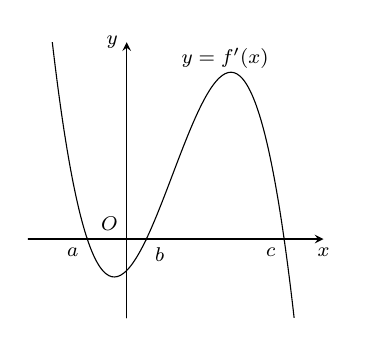
\begin{tikzpicture}[scale=0.5,line cap=round,line join=round,font=\footnotesize,>=stealth]
				\draw[->] (-2.5,0) -- (5,0) node[below]{$x$}; 
				\draw[->] (0,-2)  -- (0,5) node[left] {$y$};
				 \fill (0,0) circle (1pt) node[above left] {$O$}
					(-1,0) circle  (1pt) node[below left] {$a$}
					(0.5,0) circle (1pt) node[below  right] {$b$}
					(4,0)  circle (1pt) node[below left] {$c$};
				 \clip (-2.5,-2) rectangle (5,5);
				 \draw[smooth,samples=100,domain=-2.5:5] plot (\x,{0.4*((\x)+1)*(4-(\x))*((\x)-0.5)});
				\draw (2.5,4.6)  node{$y=f'(x)$};
			\end{tikzpicture}
		 }
	 \loigiai{
		Dựa  vào đồ thị hàm số $y=f'(x)$, ta có
		\allowdisplaybreaks 
		\begin{eqnarray*}
			\displaystyle \int_a^b f'(x) \mathrm{\,d}x < 0 &\Leftrightarrow& f(x) \Big|_a^b <0\\ 
			&\Leftrightarrow&  f(b)-f(a)<0\\
			&\Leftrightarrow& f(a)>f(b).  \quad (1)\\
			\displaystyle \int_b^c f'(x) \mathrm{\,d}x > 0 &\Leftrightarrow& f(x)  \Big|_b^c >0\\
			&\Leftrightarrow& f(c)-f(b)>0\\ 
			&\Leftrightarrow& f(c)>f(b).  \quad (2)\\
			 - \displaystyle \int_a^b f'(x) \mathrm{\,d}x < \displaystyle \int_b^c f'(x) \mathrm{\,d}x &\Leftrightarrow& -f(x) \Big|_a^b < f(x) \Big|_b^c\\
			 &\Leftrightarrow& f(a)-f(b) < f(c)-f(b)\\
			&\Leftrightarrow& f(a) < f(c). \quad  (3)
		\end{eqnarray*}
		Từ $(1)$, $(2)$ và $(3)$ suy ra $f(c)>f(a)>f(b)$. 
	 }
\end{ex}


%%%%%%%%%%%%%%%% ĐÚNG/SAI %%%%%%%%%%%%%%%%

% nguồn: Phan1_Lop_12_Dai_so_Chuong_4
\begin{ex}%[2D4H2-6]%[ma:ad76fdd8]
	Một ô tô đang chạy với tốc độ $54\,\text{ km/h}$ thì người lái xe bất ngờ phát hiện chướng ngại vật trên đường cách đó $38\,\text{ m}$. Người lái xe phản ứng một giây và sau đó đạp phanh khẩn cấp. Kể từ thời điểm này, ô tô chuyển động chậm dần đều với tốc độ $v\left( t \right) = -5t + 15\,\left( \text{ m/s} \right)$, trong đó $t$ là thời gian tính bằng giây. Gọi $s\left( t \right)$ là quãng đường xe ô tô đi được trong thời gian $t$ (giây) kể từ lúc  đạp phanh.
	 \choiceTF
		{\True Hàm số $s\left( t \right)$ được  biểu diễn bởi công thức $s\left(t \right) = -\dfrac{5}{2}t^2 + 15t$}
		{\True Thời gian kể từ lúc đạp  phanh đến khi ô tô dừng hẳn là $3$ giây}
		{Quãng đường ô tô đi được từ lúc đạp phanh đến lúc dừng hẳn là $20\,\text{ m}$} 
		{\True  Ô tô không chạm vào chướng ngại vật}
	 \loigiai{
		Đổi  $54$ km/h = $15$ m/s.
		\begin{itemchoice}
			\itemch $s(t)=\displaystyle \int v(t)\,\mathrm{d}x =\displaystyle \int \left(-5t+15\right)\,\mathrm{d}x =-\dfrac{5}{2}t^2 +  15t+C$.\\
			Vì $s(0)=0$ nên  $C=0$.\\
			Do đó hàm số  $s\left( t \right)$ được biểu diễn bởi công thức $s\left(t \right) = -\dfrac{5}{2}t^2 + 15t$.
			\itemch Khi xe dừng hẳn  thì $v(t)=0 \Leftrightarrow -5t+15=0 \Leftrightarrow t=3$.\\
			Vậy thời gian kể từ lúc đạp phanh đến khi ô tô dừng hẳn là  $3$ giây.
			\itemch Quãng đường ô tô  đi được từ lúc đạp phanh đến khi dừng hẳn là $$s_1=\displaystyle \int_0^3 v(t)\,\mathrm{d}x=\displaystyle \int_0^3 (-5t+15)\,\mathrm{d}x=22{,}5\, \text{ (m).}$$
			 \itemch
			Quãng đường ô tô đi được kể từ khi  phát hiện chướng ngại vật đến khi đạp phanh là $s_2=15 \cdot 1=15$ (m).\\
			Tổng quãng đường từ khi nhìn thấy chướng ngại vật đến khi xe dừng hẳn là $37{,}5$ (m).\\ 
			Vậy ô  tô không chạm vào chướng ngại vật.
		\end{itemchoice}
	} 
\end{ex}

% nguồn: Phan1_Lop_12_Dai_so_Chuong_4
\begin{ex}%[2D4H2-6]%[ma:f319fc96]
	Ở nhiệt độ $37^\circ$ C, một phản ứng hóa học từ chất đầu $A$, chuyển hóa thành chất sản phẩm $B$ theo phương trình $A \to B$.  Giả sử $y(x)$ là nồng độ chất $A$ (đơn vị mol $L^{-1}$) tại thời điểm $x$ (giây), $y(x)>0$ với $x \ge 0$, thỏa mãn hệ thức $y'(x)=-7\cdot 10^{-4}y(x)$ với $x \ge 0$. Biết rằng tại $x=0$, nồng độ (đầu) của $A$ là $0{,}05$ mol $L^{-1}$. Xét hàm số $f(x)=\ln y(x)$ với $x \ge 0$. Khi đó, ta có
	\choiceTF 
		{\True $f'(x)=-7\cdot 10^{-4}$} 
		{\True $f(x)=-7\cdot  10^{-4}x+\ln(0{,}05)$}
		{$y(30)-y(15)=-6\cdot  10^{-4}$}
		 {\True Nồng độ trung bình của chất $A$ từ thời điểm $15$ giây đến thời điểm $30$ giây gần bằng $0{,}05$}
	\loigiai{ 
		\begin{itemchoice}
			\itemch Ta có $f'(x)=(\ln y(x))'=\dfrac{y'(x)}{y(x)}=-7\cdot  10^{-4}$.
			\itemch Ta có $f(x)=\displaystyle\int{f'(x)\mathrm{\,d}x}=\displaystyle\int{(-7\cdot  10^{-4})\mathrm{\,d}x}=-7\cdot 10^{-4}x+C$.\\
			Theo giả thiết $y(0)=0{,}05$  nên $f(0)=\ln y(0)=\ln(0{,}05)$. Khi đó $C=\ln(0{,}05)$.\\
			 Vậy $f(x)=-7\cdot 10^{-4}x+\ln(0{,}05)$.
			\itemch  Từ $f(x)=\ln y(x) \Rightarrow y(x)=\mathrm{e}^{f(x)}=\mathrm{e}^{-7\cdot 10^{-4}x+\ln(0{,}05)}=\dfrac{1}{20}\mathrm{e}^{-7\cdot 10^{-4}x}$.\\
			Do đó $y(30)-y(15)=\left(\dfrac{1}{20}\mathrm{e}^{-7\cdot 10^{-4}\cdot 30}-\dfrac{1}{20}\mathrm{e}^{-7\cdot 10^{-4}\cdot  15}\right) \approx -5{,}2\cdot 10^{-4}$.
			\itemch Nồng độ trung bình của chất $A$ từ thời  điểm $15$ giây đến thời điểm $30$ giây là\\
			$\dfrac{1}{30-15}\displaystyle\int_{15}^{30}{y(x)\mathrm{\,d}x}=\dfrac{1}{15}\displaystyle\int_{15}^{30}{\left(-\dfrac{1}{7\cdot  10^{-4}}\right)y'(x)\mathrm{\,d}x}=-\dfrac{1}{105}y(x)\bigg|_{15}^{30}=-\dfrac{10^4}{105}[y(30)-y(15)] \approx 0{,}05$.
		\end{itemchoice}
	} 
\end{ex}

% nguồn: Phan1_Lop_12_Dai_so_Chuong_4
\begin{ex}%[2D4H2-6]%[ma:f13628d0]
	Sau khi xuất phát, ô tô di chuyển với tốc độ $v(t)=2{,}01t-0{,}025t^2$ $(0 \le t \le 10)$. Trong đó $v(t)$ tính  theo m/s, thời gian $t$ tính theo giây với $t=0$ là thời điểm xe xuất phát.
	\choiceTF 
		 {Quãng đường xe di chuyển được tính theo công thức là $s(t)=2{,}01-0{,}05t$ $(0 \le t \le 10)$}
		{\True Quãng đường xe di chuyển được trong  $3$ s là $8{,}82$ m}
		{\True Quãng đường xe  di chuyển được trong giây thứ $9$ xấp xỉ $15{,}277$ m}
		 {\True Trong khoảng thời gian không quá $10$s đầu, khi vận tốc đạt giá trị lớn nhất thì gia tốc của xe là $1{,}51$ m/s$^2$}
	 \loigiai{
		\begin{itemchoice}
			\itemch Quãng đường xe di chuyển được phải  là nguyên hàm của $v(t)$,\\
			$v'(t)=2{,}01-0{,}05t$ $(0 \le t \le 10)$ là công thức tính gia tốc của  vật.
			\itemch Quãng đường xe di chuyển được trong $3$ s  là $\displaystyle\int_{0}^{3}{(2{,}01t-0{,}025t^2)\mathrm{\,d}t}=8{,}82$ m.
			\itemch Quãng đường  xe đi chuyển được trong giây thứ $9$:\\
			$s(9)-s(8)=\displaystyle\int_{8}^{9}{(2{,}01t-0{,}025t^2)\mathrm{\,d}t}=15{,}277$ m. 
			\itemch  $v(t)=2{,}01t-0{,}025t^2$ $(0 \le t \le 10) \Rightarrow \max\limits_{[0;10]}v(t)=17{,}6$ (m/s) khi $t=10$ s.\\
			Gia tốc vật khi  đó là $a(10)=v'(10)=2{,}01-0{,}05\cdot 10=1{,}51$ (m/s$^2$).
		\end{itemchoice}
	 }
\end{ex}

% nguồn: Phan1_Lop_12_Dai_so_Chuong_4
\begin{ex}%[2D4H2-6]%[ma:dc8dc25c]
	Một chất điểm chuyển động trên đường thẳng nằm  ngang (chiều dương hướng sang phải) với gia tốc phụ thuộc vào thời gian $t$ (s) là $a(t)=2t-7$ (m/s$^2$). Biết vận tốc ban đầu bằng $6$ (m/s).
	 \choiceTF
		{Vận tốc tức thời của chất  điểm tại thời điểm $t$ s xác định bởi $v(t)=t^2-7t+10$}
		{\True Tại thời điểm $t=7$  s, vận tốc của chất điểm là $6$ (m/s)}
		{Độ dịch chuyển của vật trong khoảng thời gian $1 \le t \le 7$  là $18$ m}
		{Trong $8$ giây đầu tiên, thời điểm chất điểm xa nhất về phía bên phải là  $t=7$ s}
	 \loigiai{
		\begin{itemchoice}
			\itemch Ta có $v(t)=\displaystyle\int{a(t)\mathrm{\,d}t}=\displaystyle\int{(2t-7)\mathrm{\,d}t}=t^2-7t+C$ và $v(0)=6 \Rightarrow  C=6$.\\
			Vậy  $v(t)=t^2-7t+6$ (m/s).
			\itemch $v(7)=7^2-7\cdot 7+6=6$ (m/s). 
			\itemch Độ dịch chuyển của vật trong khoảng thời gian $1 \le t \le  7$ là\\
			$S=\displaystyle\int_{1}^{7}{v(t)\mathrm{\,d}t}=\displaystyle\int_{1}^{7}{(t^2-7t+6)\mathrm{\,d}t}=\left(\dfrac{t^3}{3}-\dfrac{7t^2}{2}+6t\right)\bigg|_{1}^{7}=-18$. 
			 \itemch Tọa độ của chất điểm tại thời điểm $t$ là\\
			$x(t)=\displaystyle\int{v(t)\mathrm{\,d}t}=\displaystyle\int{(t^2-7t+6)\mathrm{\,d}t}=\dfrac{t^3}{3}-\dfrac{7t^2}{2}+6t+C$.\\ 
			Ta  cần tìm giá trị lớn nhất của $x(t)$ với $t \in [0;8]$.\\
			Ta có $x'(t)=v(t)=0$ khi $t=1$ hoặc $t=6$.\\ 
			Lại có  $x(0)=C$, $x(1)=\dfrac{17}{6}+C$, $x(6)=-18+C$, $x(8)=-\dfrac{16}{3}+C$.\\
			Vậy giá trị lớn nhất của $x(t)$  với $t \in [0;8]$ đạt được khi $t=1$.
		\end{itemchoice}
	 }
\end{ex}

% nguồn: Phan1_Lop_12_Dai_so_Chuong_4
\begin{ex}%[2D4H2-6]%[ma:dc779d2e]
	Một ô tô đang di chuyển với  tốc độ $20$ (m/s) thì hãm phanh nên tốc độ theo thời gian $t$ được tính theo công thức $v(t)=20-5t~\left( 0\le t\le 4 \right)$. Khi đó
	\choiceTF 
		 {Sau khi hãm phanh, tốc độ của xe tăng}
		{\True Tốc độ tại thời  điểm $2$ (s) sau hãm phanh là $10$ (m/s)}
		{\True Sau khi hãm phanh  $4$ (s) thì xe dừng hẳn}
		{Kể từ khi hãm phanh đến dừng, xe đi được quãng đường $42$  (m)}
	\loigiai{ 
		\begin{itemchoice}
			\itemch Ta có $v'(t)=-5<0$ nên sau khi hãm phanh tốc  độ của xe giảm.
			\itemch Ta có $v(2)=10$  (m/s).
			\itemch Ta có $v=0 \Leftrightarrow 20-5t=0 \Leftrightarrow t=4$ (s). 
			\itemch Ta có $s=\displaystyle\int_0^4(20-5t)\mathrm{\,d}t=40$ nên kể  từ khi hãm phanh đến dừng xe đi được quãng đường $40$ (m).
		\end{itemchoice}
	} 
\end{ex}

% nguồn: Phan1_Lop_12_Dai_so_Chuong_4
\begin{ex}%[2D4H2-6]%[ma:35335b68]
	Một ô tô đang chạy với vận tốc $18$ (m/s) thì người lái hãm phanh. Sau khi hãm phanh ô tô chuyển động chậm dần đều với  vận tốc $v\left( t \right)=18-36t$ (m/s), trong đó $t$ là khoảng thời gian được tính bằng giây kể từ lúc ô tô bắt đầu hãm phanh. Khi đó
	\choiceTF 
		{Thời  gian kể từ lúc hãm phanh đến lúc xe dừng hẳn là $1{,}5$ giây}
		 {Quãng đường xe đi được sau $0{,}3$ giây kể từ lúc hãm phanh là $3$ mét}
		{\True Quãng đường kể từ lúc hãm phanh đến lúc xe dừng hẳn là $4{,}5$ mét} 
		{Gia tốc tức  thời của chuyển động này là $36~\left(\text{m/s}^2\right)$}
	 \loigiai{
		\begin{itemchoice}
			\itemch Lúc hãm phanh thì $v\left(t_1\right)=0  \Rightarrow 18-36t_1=0 \Rightarrow t_1=0{,}5$ giây.
			\itemch Quãng  đường xe đi được sau $0{,}3$ giây kể từ lúc hãm phanh là
			\[s=\displaystyle\int_0^{0{,}3} \left(  18-36t \right) \mathrm{\,d}t =\left( 18t-18t^2 \right) \Big|_0^{0{,}3}=3{,}78.\]
			 \itemch Với $t_1=0{,}5$ giây thì quãng đường kể từ lúc hãm phanh đến lúc xe dừng hẳn là
			\[s_1=\displaystyle\int_0^{0{,}5} (18-36t)\mathrm{\,d}t=\left(18t-18t^2\right)  \Big|_0^{0{,}5}=4{,}5.\]
			\itemch  Gia tốc tức thời của chuyển động này là $a=v'(t)=-36~\left(\text{m/s}^2\right)$.
		\end{itemchoice}
	} 
\end{ex}

% nguồn: Phan1_Lop_12_Dai_so_Chuong_4
\begin{ex}%[2D4H2-6]%[ma:e4af47cc]
	Một bể chứa nước có hình dạng đặc biệt đang được bơm nước vào. Biết tốc độ bơm nước $v(t)$ (đơn vị m$^3$/s) tại thời điểm $t$ (giây) được cho bởi  hàm số $v(t)=6a t^2+12t$, trong đó $a$ là hằng số. Ban đầu, trong bể đã có một lượng nước là $10$ m$^3$. Sau $3$ giây, thể tích nước trong bể là $100$ m$^3$.
	\choiceTF 
		{\True Một nguyên hàm của hàm số  $v(t)$ là $h(t)=2a t^3+6t^2$}
		{\True Lượng nước bơm  được sau $3$ giây được tính bởi công thức là $\displaystyle\int_0^3v(t) \mathrm{\,d}t$}
		{Lượng nước bơm được sau $6$  giây là $514$ m$^3$}
		{\True Thể tích nước trong bể sau khi bơm được $9$ giây là $1\,468$ m$^3$} 
	\loigiai{ 
		\begin{itemchoice}
			\itemch Ta  có $h'(t)=6at^2+12t= v(t)$ do đó $h(t)$ là một nguyên hàm của $v(t)$.
			 \itemch Lượng nước bơm được sau $3$ giây là $\displaystyle\int_0^3v(t) \mathrm{\,d}t$.
			\itemch Lượng nước trong bể sau  $t$ giây là $h(t)=2a t^3+6t^2+C$.\\
			Ban đầu bể có $10$ m$^3$ nước nên $h(0)=10\Leftrightarrow  C=10$.\\
			Sau $3$ giây trong bể có $100$ m$^3$ nước nên $h(3)=100\Leftrightarrow 27a+54+10=100\Leftrightarrow a=  \dfrac{4}{3}$.\\
			 Suy ra $h(t)=\dfrac{8}{3}t^3+6t^2+10$.\\
			Lượng nước bơm  được sau $6$ giây là $h(6)-h(0)=504$ m$^3$.
			\itemch Thể tích nước trong bể sau khi bơm được $9$  giây là $h(9)=1\,468$ m$^3$.
		\end{itemchoice}
	} 
\end{ex}

% nguồn: Phan1_Lop_12_Dai_so_Chuong_4
\begin{ex}%[2D4H2-6]%[ma:4bb5229e]
	Giả sử lợi nhuận biên (tính bằng triệu đồng) của một sản phẩm được mô hình hóa bằng công thức $P'\left( x  \right)=-0{,}0008x+10{,}4$. Ở đây $P\left( x \right)$ là lợi nhuận (tính bằng triệu đồng) khi bán được $x$ đơn vị sản phẩm. Khi đó
	 \choiceTF
		{Lợi nhuận khi bán được $x$ đơn vị sản phẩm được  tính bằng công thức \break$P\left( x \right)=-0{,}0008x^2+10{,}4x$}
		{\True  Lợi nhuận khi bán được $50$ sản phẩm đầu tiên là $519$ triệu đồng}
		{Sự thay đổi của lợi nhuận khi doanh số tăng từ $50$ lên $55$ đơn vị sản  phẩm là $49{,}79$ triệu đồng}
		{Biết sự thay đổi của lợi nhuận khi doanh số tăng từ $50$ lên $a$ đơn vị sản phẩm lớn hơn $517$  triệu đồng, khi đó giá trị nhỏ nhất của $a$ là $100$}
	 \loigiai{
		\begin{itemchoice}
			\itemch Ta có \[P(x)=\displaystyle\int P'(x)\mathrm{\,d}x=\displaystyle\int  \left( -0{,}0008x+10{,}4\right)\mathrm{\,d}x=-0{,}0004x^2+10{,}4x.\]
			 \itemch Lợi nhuận khi bán được $50$ sản phẩm đầu tiên là
			\[P(50)=-0{,}0004\cdot  50^2+10{,}4\cdot 50=519~(\text{triệu đồng}).\]
			\itemch Sự thay  đổi của lợi nhuận khi doanh số tăng từ $50$ lên $55$ đơn vị sản phẩm là
			\begin{eqnarray*}
				P(55)-P(50)&=&\displaystyle\int_{50}^{55}  P'(x)\mathrm{\,d}x\\
				 &=&\displaystyle\int_{50}^{55} \left( -0{,}0008x+10{,}4 \right)\mathrm{\,d}x\\
				&=&-\displaystyle\int_{50}^{55}  0{,}0008x\mathrm{\,d}x+\displaystyle\int_{50}^{55} 10{,}4\mathrm{\,d}x\\
				&=&  -0{,}0004x^2 \Big|_{50}^{55}+ 10{,}4x \Big|_{50}^{55}\\
				&=&  -0{,}0004\left( 55^2-50^2 \right)+10{,}4(55-50)\\
				 &=& 51{,}79~(\text{triệu đồng}).
			\end{eqnarray*}
			\itemch Sự thay đổi của lợi nhuận khi doanh số tăng từ $50$ lên $a$ đơn vị sản phẩm là 
			\begin{eqnarray*}
				P(a)-P(50)&=&\displaystyle\int_{50}^a  P'(x)\mathrm{\,d}x\\
				&=&  \displaystyle\int_{50}^a \left( -0{,}0008x+10{,}4 \right)\mathrm{\,d}x\\
				&=&-\displaystyle\int_{50}^a 0{,}0008x\mathrm{\,d}x+\displaystyle\int_{50}^a 10{,}4\mathrm{\,d}x\\ 
				&=& -0{,}0004x^2  \Big|_{50}^a+ 10{,}4x \Big|_{50}^a\\
				&=& -0{,}0004\left(a^2-50^2  \right)+10{,}4(a-50)\\
				&=&  -0{,}0004a^2+10{,}4a-519.
			\end{eqnarray*}
			Theo bài ra,  ta có
			\begin{eqnarray*}
				&&-0{,}0004a^2+10{,}4a-519>517 \\ 
				 &\Leftrightarrow& 0{,}0004a^2-10{,}4a+1036<0\\
				&\Leftrightarrow& 100<a<25\,900. 
			\end{eqnarray*}
			Vậy giá trị nhỏ nhất của $a$  là $101$.
		\end{itemchoice}
	 }
\end{ex}

% nguồn: Phan1_Lop_12_Dai_so_Chuong_4
\begin{ex}%[2D4H2-6]%[ma:b13f27ef]
	Tại một nhà máy sản xuất một loại phân bón. Gọi $P(x)$ là lợi nhuận (tính theo triệu đồng) thu được từ việc bán $x$ (tấn) sản phẩm trong một tuần. Khi đó đạo hàm $P'(x)$ gọi là lợi nhuận cận biên, cho biết tốc độ tăng lợi nhuận theo lượng sản phẩm bán được. Giả sử lợi nhuận cận biên (tính theo triệu đồng trên tấn) của nhà máy được ước lượng bởi công thức $P'(x)=17-0{,}025x$ với $0\le x\le 100$. Biết nhà máy lỗ $24$ triệu đồng nếu không bán được  lượng sản phẩm nào trong tuần. Khi đó
	\choiceTF 
		{Công thức lợi nhuận (tính theo triệu đồng) thu được từ việc bán $x$ (tấn)  sản phẩm trong một tuần là $P(x)=17x-0{,}0125x^2+C$ với $C$ là một hằng số bất kỳ}
		{Có thể tính được lợi nhuận của nhà máy thu  được khi bán $120$ tấn sản phẩm trong tuần}
		{\True Lợi nhuận nhà máy thu được khi bán $80$ tấn sản phẩm trong  tuần là $1$ tỉ $256$ triệu đồng}
		{Nếu nhà  máy bán được từ $1{,}3$ tấn sản phẩm trên tuần trở lên thì nhà máy luôn có lãi}
	\loigiai{ 
		\begin{itemchoice}
			\itemch Ta có $P(x)=\displaystyle\int P'(x)\mathrm{\,d}x=\displaystyle\int \left( 17-0{,}025x \right)\mathrm{\,d}x=17x-0{,}0125x^2+C$ với  $0\le x\le 100$.\\
			Vì nhà máy lỗ $24$ triệu đồng nếu không  bán được lượng sản phẩm nào trong tuần nên $x=0$ thì
			 \[P(0)=-24\Leftrightarrow C=-24\Rightarrow P(x)=17x-0{,}0125x^2-24.\]
			Vậy $C=-24$ không phải $C$ bất kỳ! 
			\itemch Công thức $P'(x)$ đề cho chỉ áp dụng được khi $0\le x\le 100$. 
			\itemch Khi bán $80$ tấn sản phẩm trong tuần thì $x=80$ và  $P(80)=1\,256$ triệu đồng.
			\itemch Nhà máy  chỉ bắt đầu có lãi khi
			 \[P(x)>0 \Rightarrow 17x-0{,}0125x^2-24>0 \Rightarrow 1{,}41<x<1\,358{,}5.\]
			 Vậy nếu $1{,}3\le x\le 1{,}41$ nhà máy vẫn có thể bị lỗ.
		\end{itemchoice}
	} 
\end{ex}

% nguồn: Phan1_Lop_12_Dai_so_Chuong_4
\begin{ex}%[2D4H2-6]%[ma:3c0ca08b]
	Ở nhiệt độ $37^\circ C$, một phản ứng hóa học từ chất đầu $A$, chuyển hóa thành chất sản phẩm $B$ theo phương trình $A\to B$. Giả sử $y(x)$ là nồng  độ chất $A$ (đơn vị mol L$^{-1}$) tại thời điểm $x$ (giây), $y(x)>0$ với $x\ge 0$ thỏa mãn hệ thức $y'(x)=-7\cdot 10^{-4}y(x)$ với $x\ge 0$. Biết rằng tại $x=0$ nồng độ (đầu) của $A$ là $0{,}05$ mol L$^{-1}$. Xét hàm số $f(x)=\ln y(x)$ với $x\ge 0$. Khi đó
	\choiceTF 
		{\True $f'(x)=-7\cdot  10^{-4}$}
		 {\True $f(x)=-7\cdot 10^{-4}x+\ln\left( 0{,}05 \right)$}
		{$y(30)-y(15)=-6\cdot  10^{-4}$}
		{\True Nồng độ trung bình của chất $A$ từ thời điểm $15$  giây đến thời điểm $30$ giây gần bằng $0{,}05$}
	 \loigiai{
		\begin{itemchoice}
			\itemch Ta có $f'(x)= \big[\ln y(x)\big]'=\dfrac{y'(x)}{y(x)}=-7\cdot  10^{-4}$.
			\itemch Ta có  $f(x)=\displaystyle\int f'(x)\mathrm{\,d}x=\displaystyle\int \left(-7\cdot 10^{-4}\right)\mathrm{\,d}x=-7\cdot 10^{-4}x+C$.\\
			Theo giả thiết $y(0)=0{,}05$ nên $f(0)=\ln y(0)=\ln\left( 0{,}05  \right)$.\\
			Khi đó $C=\ln\left(  0{,}05 \right)$.\\
			Vậy $f(x)=-7\cdot 10^{-4}x+\ln\left(  0{,}05 \right)$.
			\itemch Từ $f(x)=\ln y(x) \Rightarrow y(x)=\mathrm{e}^{f(x)}=\mathrm{e}^{-7\cdot 10^{-4}x+\ln\left( 0{,}05  \right)}=\dfrac{1}{20}\mathrm{e}^{-7\cdot 10^{-4}x}$.\\
			Do đó $y(30)-y(15)=\dfrac{1}{20}\left(\mathrm{e}^{-7\cdot 10^{-4}\cdot 30}-\mathrm{e}^{-7\cdot 10^{-4}\cdot 15} \right)\approx -5{,}2\cdot 10^{-4}$. 
			\itemch Nồng  độ trung bình của chất $A$ từ thời điểm $15$ giây đến thời điểm $30$ giây là
			\begin{eqnarray*}
				\dfrac{1}{30-15}\displaystyle\int_{15}^{30} y(x)\mathrm{\,d}x 
				 &=& \dfrac{1}{15}\displaystyle\int_{15}^{30} \left(-\dfrac{1}{7\cdot 10^{-4}}\right)y'(x)\mathrm{\,d}x\\
				&=&-\dfrac{10^4}{105}y(x)\bigg|^{30}_{15}\\ 
				 &=&-\dfrac{10^4}{105}\big[y(30)-y(15)\big]\\
				 &\approx& 0{,}05.
			\end{eqnarray*}
		\end{itemchoice}
	 }
\end{ex}

% nguồn: Phan1_Lop_12_Dai_so_Chuong_4
\begin{ex}%[2D4H2-6]%[ma:f97781b2]
	Sau khi xuất phát, ô tô di chuyển với tốc độ $v(t)=2{,}01t-0{,}025t^2~(0\le t\le 10)$. Trong đó $v(t)$ tính theo (m/s), thời gian  $t$ tính theo $s$ với $t=0$ là thời điểm xe xuất phát. Khi đó
	\choiceTF 
		{Quãng đường xe di chuyển được tính theo công thức là $s\left( t \right)=2{,}01-0{,}05t$,  $(0\le t\le 10)$}
		{\True Quãng đường xe di chuyển được trong  $3$ s là $8{,}82$ m}
		 {\True Quãng đường xe di chuyển được trong giây thứ $9$ xấp xỉ $15{,}277$ m}
		{\True Trong khoảng thời gian không quá $10$ s đầu, khi vận tốc đạt giá trị lớn nhất thì gia tốc của xe  là $1{,}51$ m/s$^2$}
	\loigiai{ 
		\begin{itemchoice}
			\itemch Quãng đường xe  di chuyển được phải là nguyên hàm của $v(t)$.\\
			Khi  đó $v'(t)=2{,}01-0{,}05t~(0\le t\le 10)$ là công thức tính gia tốc của vật.
			\itemch Quãng đường xe di chuyển được trong $3$ s  là
			\[\displaystyle\int_0^3  \left(2{,}01t-0{,}025t^2\right)\mathrm{\,d}t=8{,}82~\text{ (m)}.\]
			\itemch Quãng đường xe di chuyển được trong giây thứ $9$  là
			\[s(9)-s(8)=\displaystyle\int_8^9 \left( 2{,}01t-0{,}025t^2 \right)\mathrm{\,d}t\approx  15{,}277~\text{ (m)}.\]
			\itemch Ta có $v(t)=2{,}01t-0{,}025t^2~(0\le t\le  10)$.\\
			Suy ra $\max\limits_{[0;10]}  v(t)=17{,}6~\text{ (m/s)}$ khi $t=10$ s.\\
			Gia tốc vật khi đó  là $a(10)=v'(10)=2{,}01-0{,}05\cdot 10=1{,}51~\left(\text{m/s}^2\right)$.
		\end{itemchoice}
	} 
\end{ex}

% nguồn: Phan1_Lop_12_Dai_so_Chuong_4
\begin{ex}%[2D4H2-6]%[ma:179109be]
	Giả sử lợi nhuận biên (tính triệu đồng) của một sản phẩm được mô hình hóa bằng công  thức $P'(x)=-0{,}0008x+10{,}4$. Ở đây $P(x)$ là lợi nhuận (tính bằng triệu đồng) khi bán được $x$ đơn vị sản phẩm.
	 \choiceTF
		{Lợi nhuận khi bán được $x$ đơn vị sản phẩm  được tính bằng $P(x)=-0{,}0008x^2+10{,}4x$}
		{\True Lợi nhuận khi bán  được $50$ sản phẩm đầu tiên là $519$ triệu đồng}
		{Sự thay đổi  của lợi nhuận khi doanh số tăng từ $50$ lên $55$ đơn vị sản phẩm là $49{,}79$ triệu đồng}
		{Biết sự thay đổi của lợi nhuận khi doanh số tăng từ $50$ lên $a$ đơn vị sản phẩm lớn hơn $517$ triệu đồng, khi đó giá  trị nhỏ nhất của $a$ là $100$}
	 \loigiai{
		\begin{itemchoice}
			\itemch Ta có $P(x)=\displaystyle\int{P'(x)\mathrm{\,d}x}=\displaystyle\int{(-0{,}0008x+10{,}4)\mathrm{\,d}x}=-0{,}0004x^2+10{,}4x$. 
			\itemch Lợi nhuận khi  bán được $50$ sản phẩm đầu tiên là\\
			$P(50)=-0{,}0004\cdot  50^2+10{,}4\cdot 50=519$ (triệu đồng).
			\itemch Ta có sự thay đổi của lợi nhuận khi doanh số tăng  từ $50$ lên $55$ đơn vị sản phẩm là\\
			 $P(55)-P(50)=\displaystyle\int_{50}^{55}{P'(x)\mathrm{\,d}x}=\displaystyle\int_{50}^{55}{(-0{,}0008x+10{,}4)\mathrm{\,d}x}=\displaystyle\int_{50}^{55}{-0{,}0008x\mathrm{\,d}x}+\displaystyle\int_{50}^{55}{10{,}4\mathrm{\,d}x}$\\
			$=-0{,}0004x^2\bigg|_{50}^{55}+10{,}4x\bigg|_{50}^{55}=-0{,}0004(55^2-50^2)+10{,}4(55-50)=51{,}79$  (triệu đồng).
			\itemch Ta có sự thay đổi của lợi nhuận khi doanh số tăng từ $50$ lên $a$ đơn  vị sản phẩm là\\
			 $P(a)-P(50)=\displaystyle\int_{50}^{a}{P'(x)\mathrm{\,d}x}=\displaystyle\int_{50}^{a}{(-0{,}0008x+10{,}4)\mathrm{\,d}x}=\displaystyle\int_{50}^{a}{-0{,}0008x\mathrm{\,d}x}+\displaystyle\int_{50}^{a}{10{,}4\mathrm{\,d}x}$\\
			 $=-0{,}0004x^2\bigg|_{50}^{a}+10{,}4x\bigg|_{50}^{a}=-0{,}0004(a^2-50^2)+10{,}4(a-50)=-0{,}0004a^2+10{,}4a-519$.\\
			Theo bài ra  ta có\\
			$-0{,}0004a^2+10{,}4a-519 >  517 \Leftrightarrow 0{,}0004a^2-10{,}4a+1036 < 0 \Leftrightarrow 100 < a < 25900$.\\
			Vậy  giá trị nhỏ nhất của $a$ là $101$.
		\end{itemchoice}
	} 
\end{ex}

% nguồn: Phan1_Lop_12_Dai_so_Chuong_4
\begin{ex}%[2D4H2-6]%[ma:5c994190]
	Giả sử chi phí mua và bảo trì một thiết bị trong $x$ năm có thể được mô hình hóa theo công  thức $C=5\,000\left( 25+3\displaystyle\int_0^x t^{\tfrac{1}{4}}\mathrm{\,d}t \right)$. Khi đó
	\choiceTF 
		{Chi phí mua $1$ sản  phẩm là $100\,000$ đồng}
		{\True Chi phí bảo  trì năm đầu tiên của $1$ sản phẩm là $12\,000$ đồng}
		{Sau $6{,}5$ năm thì số tiền  mua một sản phẩm bằng số tiền bảo trì sản phẩm đó}
		{Nếu một nhà đầu tư có $10$ triệu thì họ có thể mua và bảo trì tối đa $30$ sản  phẩm trong $10$ năm}
	\loigiai{ 
		\begin{itemchoice}
			\itemch Chi phí mua $1$ sản phẩm ứng với $x=0$, sau ra $C=5\,000\cdot 25=125\,000$. 
			\itemch Với $x=1$ ta có  $C=5\,000\left( 25+3\displaystyle\int_0^1 t^{\tfrac{1}{4}}\mathrm{\,d}t \right)=137\,000$.\\
			Suy ra chi phí bảo trì năm đầu tiên của  sản phầm là
			\[137\,000-125\,000=12\,000~ \text{ đồng}.\] 
			\itemch Gọi $x$  là số năm mà số tiền bảo trì bằng số tiền mua sản phẩm. Khi đó tổng số tiền mua và số tiền bảo trì là $2\cdot 125\,000=250\,000$.\\
			 Ta có
			\begin{eqnarray*}
				&& 5\,000\left( 25+3\displaystyle\int_0^x  t^{\tfrac{1}{4}}\mathrm{\,d}t \right)=250\,000\\
				&\Leftrightarrow& 25+3\left( \dfrac{4}{5} t^{\tfrac{5}{4}}\Big|_0^x  \right)=50\\
				&\Leftrightarrow& \dfrac{12}{5}  x^{\tfrac{5}{4}}=25\\
				&\Leftrightarrow& x=\left( \dfrac{75}{2}  \right)^{\tfrac{4}{5}} \approx 6{,}52.
			\end{eqnarray*}
			\itemch Số tiền mua và bảo trì $1$ sản  phẩm trong $10$ năm là
			$$C=5\,000\left( 25+3\displaystyle\int_0^{10} t^{\tfrac{1}{4}}\mathrm{\,d}t  \right)=5\,000\left( 25+24\sqrt[4]{10} \right) \approx 338\,393{,}53.$$
			Ta  có $\dfrac{10\,000\,000}{338\,393{,}53} \approx 29{,}55.$\\
			Vậy với $10$ triệu  thì họ có thể mua và bảo trì tối đa $29$ sản phẩm trong $10$ năm.
		\end{itemchoice}
	 }
\end{ex}

% nguồn: Phan1_Lop_12_Dai_so_Chuong_4
\begin{ex}%[2D4V2-6]%[ma:23cf1971]
	Giả sử rằng khi $t$ năm tuổi, một  máy công nghiệp $A$ tạo ra doanh thu với tốc độ $R'(t)=588 - 3t^2$ (triệu đồng/năm), tính từ lúc bắt đầu hoạt động ($t=0$). Biết chi phí biên vận hành và bảo trì là $C'(t)=48 + 12t^2$ (triệu đồng/năm), với $C(t)$ là chi phí vận hành và bảo trì của máy $A$ khi nó được $t$ năm tuổi.
	\choiceTF 
		{\True $C(t)=\displaystyle\int(48 + 12t^2)\,\mathrm{\,d}t$} 
		{$C(t)=48t + 4t^3  + 20$}
		{\True Tổng chi phí vận hành và bảo trì trong $6$ năm của  máy $A$ là $1\,152$ (triệu đồng)}
		{\True Lợi nhuận do máy $A$ tạo ra trong suốt thời gian tuổi thọ  hữu ích là $2\,160$ (triệu đồng), với tuổi thọ hữu ích là thời gian trước khi lợi nhuận bắt đầu giảm}
	 \loigiai{
		\begin{itemchoice}
			\itemch Ta có 
			\[C(t)=\displaystyle \int C'(t)\,\mathrm{\,d}t=\int(48 + 12t^2)\,\mathrm{\,d}t.\] 
			 \itemch Ta có
			\[C(t)=\displaystyle \int(48  + 12t^2)\,\mathrm{\,d}t=4t^3+48t+C.\]
			Vì $C(0)=0$  nên
			\[4 \cdot  0^3 +48 \cdot 0 +C=0 \Leftrightarrow C=0.\]
			Vậy  $C(t)=48t + 4t^3$.
			\itemch Tổng chi phí vận hành và bảo trì trong $6$ năm của máy $A$  là
			\[\displaystyle  \int_0^6 \left(48 + 12t^2\right) \mathrm{\,d}t=1\,152 \ (\text{triệu đồng}).\]
			\itemch Doanh thu của một máy công nghiệp $A$ khi  $t$ năm tuổi là
			 \[R(t) =\displaystyle \int (588-3t^2) \mathrm{\,d}t=-t^3+588t+C.\]
			Vì $R(0)=0$  nên
			\[-0^3+588\cdot 0  +C=0 \Leftrightarrow C=0.\]
			 Vậy $R(t)=-t^3+588t$.\\
			Lợi nhuận của một máy công nghiệp $A$  khi $t$ năm tuổi là
			 \[P(t)=R(t)-C(t)=-t^3+588t-4t^3-48t=-5t^3+540t.\]
			 Ta có
			\[P'(t)=-15t^2+540=0 \Leftrightarrow \hoac{&t=6\\&t=-6.}\] 
			Bảng xét  dấu
			\begin{center}
				
\begin{tikzpicture}[>=stealth]
						 \tkzTabInit[lgt=1.2,espcl=3]
						 {$t$ /1,$P'(t)$ /1}
						 {$0$,$6$,$+\infty$}
						\tkzTabLine{,+,0,-,} 
					\end{tikzpicture}
			\end{center}
			Thời gian tuổi thọ hữu ích của máy $A$ là $6$  năm.\\
			Lợi nhuận do máy  $A$ tạo ra trong suốt thời gian tuổi thọ hữu ích là
			\[\displaystyle  \int_0^6 \left(-15t^2+540\right)\mathrm{\,d}t=2\,160 \ (\text{Triệu đồng}).\]
	\end{itemchoice}}
\end{ex}

% nguồn: Phan1_Lop_12_Dai_so_Chuong_4
\begin{ex}%[2D4V2-6]%[ma:95419aee]
	Một vật chuyển động với  vận tốc được cho bởi đồ thị trong hình sau:
	\begin{center}
		\begin{tikzpicture}
				\draw[->] (0,-0.5) -- (0,3) node[above left] {$v (\text{m/s})$}; 
				\draw[->] (-0.5,0) -- (3,0) node[above right]  {$t (\text{s})$};
				\node  at (0,0) [below left] {O};
				\coordinate (O)  at (0,0);
				\coordinate (A)  at (1,2);
				\coordinate (B) at (2,2); 
				 \draw (O) -- (A);
				\draw (A)  -- (B);
				\fill (A) circle (1.5pt) node[above right]  {A};
				\fill  (B) circle (1.5pt) node[above right] {B};
				\draw[dashed] (A) -- (1,0) node[below]  {1};
				\draw[dashed] (A)  -- (0,2) node[left] {2};
				\draw[dashed] (B) -- (2,0) node[below] {2}; 
			\end{tikzpicture}
	\end{center}
	 \choiceTF
		{\True Vận tốc của vật tại thời điểm $t$ được xác định bởi $v(t)=\heva{&2t \text{ khi }0\le t\le 1 \\&2 \text{ khi  }t>1}$}
		{\True Quãng đường vật đi được  trong $1$ giây đầu tiên được xác định bởi công thức \break $\displaystyle s(t)=\int_0^1 v(t)\mathrm{\,d}t$}
		{Quãng  đường vật đi được trong khoảng thời gian từ $1$ giây đến $2$ giây được xác định bởi công thức $\displaystyle s(t)=\int_0^2 v(t)\mathrm{\,d}t$}
		{\True Quãng đường mà vật  đi được trong $2$ giây đầu tiên là $3$ m}
	\loigiai{ 
		\begin{itemchoice}
			\itemch Ta có phương trình đường thẳng đi qua hai điểm $O$, $A$ là $y=2x$,  đường thẳng đi qua hai điểm $A$, $B$ là $y=2$.\\
			Do đó ta có công thức  hàm vận tốc là $v(t)=\heva{&2t &\text{ khi }0\le t\le 1 \\&2 &\text{ khi }t>1.}$\\
			Quãng đường vật đi được trong khoảng thời gian từ $a$ giây đến $b$ giây được  xác định bởi công thức $\displaystyle s(t)=\int_a^bv(t)\mathrm{\,d}t$.
			\itemch Do đó quãng đường vật đi  được trong khoảng thời gian từ $0$ giây đến $1$ giây được xác định bởi công thức $\displaystyle s(t)=\int_0^1 v(t)\mathrm{\,d}t$.
			\itemch Quãng đường vật đi được trong khoảng thời gian từ $1$ giây đến $2$ giây được xác định  bởi công thức $\displaystyle s(t)=\int_1^2 v(t)\mathrm{\,d}t$.
			 \itemch Quãng đường mà vật đi được trong $2$ giây đầu tiên là
			\begin{center}
				$\displaystyle  s(t)=\int_0^2 v(t)\mathrm{\,d}t
				=\int_0^12t\mathrm{\,d}t+\int_1^22\mathrm{\,d}t 
				=t^2\bigg|_0^1+2t\bigg|_1^2=1+2=3$ m. 
			\end{center}
		\end{itemchoice}
	 }
\end{ex}

% nguồn: Phan1_Lop_12_Dai_so_Chuong_4
\begin{ex}%[2D4V2-6]%[ma:a043f5a5]
	Một chất điểm chuyển động trên đường thẳng nằm ngang (chiều dương hướng sang phải) với gia tốc phụ thuộc vào thời gian $t$ (s) là $a(t)=2t-7$ m/s$^2$. Biết vận tốc đầu bằng $6$ m/s. 
	 \choiceTF
		{Vận tốc tức thời của chất điểm tại thời điểm $t$ (s) xác  định bởi $v(t)=t^2-7t+10$}
		{\True Tại thời điểm $t=7$  s, vận tốc của chất điểm là $6$ m/s}
		{Độ dịch chuyển của vật trong khoảng thời gian $1 \le t \le 7$ là $18$ m} 
		{Trong $8$ giây đầu tiên, thời điểm chất điểm xa nhất về phía  bên phải là $t=7$ s}
	\loigiai{ 
		\begin{itemchoice}
			\itemch 
			$v(t)=\displaystyle\int  a(t) \mathrm{\,d}t=t^2-7t+C$.\\
			Khi $t=0$ thì $v=6$  m/s, suy ra $v(0)=6 \Rightarrow C=6$.\\
			Vậy $v(t)=t^2-7t+6$ m/s. 
			\itemch Ta có  $v(7)=7^2-7\cdot7+6=49-49+6=6$ m/s.
			\itemch Độ dịch chuyển $\Delta  s=s(7)-s(1)=\displaystyle\int_1^7 v(t) dt=\displaystyle\int_1^7 (t^2-7t+6) \mathrm{\,d}t=-18\ne 18$.
			 \itemch Độ dịch chuyển là\\
			$d(t)=\displaystyle\int v(t)\,\mathrm{d}t=\dfrac{t^3}{3}-\dfrac{7t^2}{2}+6t+C$. \\ 
			$d(0)=0  \Rightarrow C=0$.\\
			$\Rightarrow  d(t)=\dfrac{t^3}{3}-\dfrac{7t^2}{2}+6t$
			 Ta có
			\begin{eqnarray*}
				&& d'(t)=0 \Leftrightarrow v(t)=0 \\ 
				&& \Leftrightarrow t^2-7t+6=0  \\
				&& \Leftrightarrow (t-6)(t-1)=0 \\ 
				&& \Leftrightarrow t=1 \text{  hoặc } t=6.
			\end{eqnarray*}
			Bảng biến  thiên
			\begin{center}
				
\begin{tikzpicture}
						\tkzTabInit[lgt=1.2,espcl=3]{$t$/1,$d'(t)$ /1,$d  (t)$/2}
						 {$0$,$1$,$6$,$8$}
						\tkzTabLine{6,+,0,-,0,+} 
						\tkzTabVar{-/ $d (0)$,+/ $d (1)$,-/ $d  (6)$,+/ $d (8)$}
					\end{tikzpicture}
			\end{center}
			$d(1)=\dfrac{1^3}{3}-\dfrac{7\cdot1^2}{2}+6\cdot1=2{,}83$,\\ 
			$d(8)=\dfrac{8^3}{3}-\dfrac{7\cdot8^2}{2}+6\cdot8=-5{,}33$.\\ 
			Vậy thời điểm chất điểm xa nhất về phía bên phải trong khoảng $0 \le  t \le 8$ là $t=1$.
		\end{itemchoice}
	} 
\end{ex}

% nguồn: Phan1_Lop_12_Dai_so_Chuong_4
\begin{ex}%[2D4V2-6]%[ma:643eba8a]
	Một chất điểm chuyển động thẳng trong $24$ giây với vận tốc $v(t)$ (đơn vị: m/s) là hàm số phụ thuộc thời gian $t$ (đơn vị:  giây) có đồ thị cho bởi hình vẽ sau:
	\begin{center}
		\begin{tikzpicture}[scale=0.15,font=\footnotesize,line join=round,line cap=round,>=stealth]
				 \def \xmin{-4}
				 \def \xmax{27}
				 \def \ymin{-4}
				\def  \ymax{34}
				\draw[teal,->] (\xmin,0)--(\xmax,0) node[above] {$t$}; 
				 \draw[teal,->] (0,\ymin)--(0,\ymax) node[right] {$v (t)$};
				\fill (0,0) circle (5pt) node [below left] {$O$}; 
				\foreach \x in {2,16,24} \fill (\x,0) circle (5pt) node [below] {$\x$}; 
				\foreach  \y in {10,30} \fill (0,\y) circle (5pt) node [left] {$\y$};
				 \fill (2,10) circle (5pt)
					 (16,30) circle (5pt)
					 (2,10) circle (5pt)
					(24,0)  circle (5pt);
				 \draw[teal] (0,10)--(2,10)--(16,30)--(24,0);
				 \draw[teal,dashed] (2,0)--(2,10)
					 (0,30)--(16,30)--(16,0);
			\end{tikzpicture}
	\end{center}
	\choiceTF 
		{\True Tại thời  điểm $t=2$ giây, vận tốc của chất điểm bằng $10$\,m/s}
		{\True Trong  khoảng thời gian từ $2$ giây đến $16$ giây, đồ thị của $v(t)$ là một phần của đường thẳng có phương trình $v(t)=\dfrac{10}{7}t+\dfrac{50}{7}$\,m/s}
		{Quãng đường $s(t)$ (đơn vị: mét) mà chất điểm đi được trong  khoảng thời gian $t$ giây\break ($0\leq t\leq 24$) được tính theo công thức $s(t)=\displaystyle\int_0^t \left(\dfrac{10}{7}t+\dfrac{50}{7}\right)\mathrm{\,d}t$}
		{\True Quãng đường chất điểm đi được từ lúc $0$ giây đến $24$  giây bằng $420$\,m}
	 \loigiai{
		\begin{itemchoice}
			\itemch 
			Dựa vào đồ thị, tại thời điểm $t=2$ giây thì vận tốc của chất điểm là  $v(2)=10$\,(m/s).
			 \itemch
			Dựa vào đồ thị, trong khoảng thời gian từ  $2$ giây đến $16$ giây thì $v(2)=10$ và $v(16)=30$.\\
			Trong  đoạn $t\in [2;16]$, vận tốc $v(t)$ có dạng $v(t)=at+b$.\\
			Đồ thị $v(t)$ đi qua $2$ điểm có  tọa độ $(2;10)$ và $(16;30)$ nên ta có hệ phương trình
			 \[\heva{&2a+b=10\\&16a+b=30}\Leftrightarrow\heva{&a=\dfrac{10}{7}\\&b=\dfrac{50}{7}.}\]
			Vậy phương trình vận tốc trong khoảng thời gian từ $2$ giây đến $16$  giây là
			\[v(t)=\dfrac{10}{7}t+\dfrac{50}{7}\,\text{ (m/s)}.\] 
			\itemch Dựa vào đồ thị,  trong khoảng thời gian $t$ giây
			\begin{itemize}
				\item Với $t\in  [0;2]$ thì quãng đường chuyển động là $s(t)=10t$ (m);
				\item Với $t\in  [2;16]$ thì quãng đường chuyển động là $s(t)=20+\displaystyle\int_2^t \left(\dfrac{10}{7}x+\dfrac{50}{7}\right)\mathrm{d}x$ (m);
				\item Với $t\in [16;24]$ thì vận tốc được xác định bởi công thức 
				 $v(t)=mt+n$.\\
				Ta có  $\heva{&16m+n=30\\&24m+n=0}\Leftrightarrow\heva{&m=-\dfrac{15}{4}\\&n=90.}$\\
				Suy ra  $v(t)=-\dfrac{15}{4}t+90$.\\
				Khi đó, quãng  đường chuyển động là $s(t)=300+\displaystyle\int_{16}^{t} \left(-\dfrac{15}{4}x+90\right)\mathrm{d}x$ (m).
			\end{itemize}
			 \itemch Dựa vào đồ thị, trong khoảng thời gian
			\begin{itemize}
				\item Từ $0$ giây đến $2$ giây thì phương trình  đường thẳng có dạng là $v(t)=10$\,(m/s).
				\item Từ $2$ giây đến $16$ giây thì phương trình đường thẳng có dạng là $v(t)=\dfrac{10}{7}t+\dfrac{50}{7}$\,(m/s). 
				\item Từ $16$ giây đến $24$ giây thì phương trình đường thẳng  có dạng là \break $v(t)=-\dfrac{15}{4}t+90$\,(m/s).
			\end{itemize}
			Vậy quãng đường mà chất điểm đi được trong  khoảng thời gian $24$ giây là \[s(t)=\displaystyle\int_0^2 10 \mathrm{\,d}t+\displaystyle\int_2^{16} \left(\dfrac{10}{7}t+\dfrac{50}{7}\right)\mathrm{\,d}t+\displaystyle\int_{16}^{24} \left(-\dfrac{15}{4}t+90\right)\mathrm{\,d}t=420 \text{ (m).}\]
		\end{itemchoice}
	} 
\end{ex}

% nguồn: Phan1_Lop_12_Dai_so_Chuong_4
\begin{ex}%[2D4V2-6]%[ma:c72ae3f3]
	\immini{Một vật chuyển động với vận tốc  $y=v(t)$ (m/s) được cho bởi đồ thị như hình vẽ bên dưới. Trong thời gian 3 giây kể từ khi bắt đầu chuyển động, đồ thị đó là một phần của đường parabol có đỉnh $I(2;4)$, khoảng thời gian còn lại đồ thị là đoạn thẳng song song trục hoành.
	 \choiceTF
		{\True Vận tốc không đổi trong khoảng thời gian từ $3$ giây đến $5$  giây}
		{\True Trong $3$ giây đầu tiên thì $v(t)=-t^2+4t$} 
		{\True Quãng đường mà  vật di chuyển trong 3 giây đầu được tính bởi công thức $\displaystyle\int_0^3\left(-t^2+4t\right) \mathrm{\,d}t$}
		{Quãng đường mà vật di chuyển trong $5$ giây kể từ khi bắt đầu chuyển  động bằng $\dfrac{250}{3}$ (m)}}
		{\begin{tikzpicture}[>=stealth,x=1cm,y=1cm,scale=0.8]
		 \def\a{-1}
		 \def\b{4}
		\def\c{0} 
		 \draw[->] (-1,0) -- (6,0) node[below] {$t$};
		\draw[->]  (0,-1) -- (0,5) node[left] {$v$};
		\draw (0,0)  node[below left]{$O$}
			(3,0) node[below]{$3$} 
			 (4,0) node[below]{$4$}
			(2,0)  node[below]{$2$}
			 (0,4) node[left]{$4$};
		 \pgfmathsetmacro\xdinh{-(\b)/2*(\a)}
		\pgfmathsetmacro\ydinh{(4*(\a)*(\c)-(\b)^2)/(4*(\a))} 
		\fill[dashed] (2,4) circle (2pt) edge  (2,0) edge (0,4)
			(3,3) circle (2pt)  edge (3,0)
			(5,3) circle (2pt) edge  (5,0)
			(4,0)  circle (1.0pt);
		\draw[samples=200,smooth,domain=0:3] plot  (\x,{\a*(\x)^2+(\b)*\x+(\c)});
		\draw (3,3)--(5,3) 
			(5,0) node[below]{$5$}; 
	\end{tikzpicture}}
	\loigiai{ 
		\begin{itemchoice}
			 \itemch \textbf{Đúng}.\\
			Vận tốc không đổi trong khoảng thời gian  từ $3$ giây đến $5$ giây.
			\itemch  \textbf{Đúng}.\\
			Giả sử phương trình vận  tốc của vật là $v(t)=at^2+bt+c\ (a\ne 0)$.\\
			Ta có $\heva{&c=0\\&4a+2b+c=4\\&-\dfrac{b}{2a}=2}\Leftrightarrow  \heva{&c=0\\&b=4\\&a=-1}\Leftrightarrow v(t)=-t^2+4t$.
			\itemch \textbf{Đúng}.\\ 
			Quãng  đường mà vật di chuyển trong 3 giây đầu được tính bởi công thức $\displaystyle\int_0^3\left(-t^2+4t\right) \mathrm{\,d}t$
			 \itemch \textbf{Sai}.\\
			Ta có $v(3)=3$ suy ra phương trình chuyển động của vận tốc  trên khoảng từ $3$ đến $5$ giây là $v=3$.\\
			Vậy quãng đường mà vật di  chuyển trong $5$ giờ là
			$\displaystyle\int_{0}^{3} (-t^2+4t) \mathrm{\,d}t+\displaystyle\int_{3}^{5} 3  \mathrm{\,d}t =15$ (km).
		\end{itemchoice}
	} 
\end{ex}

% nguồn: Phan1_Lop_12_Dai_so_Chuong_4
\begin{ex}%[2D4V2-6]%[ma:b45b9385]
	Giả sử tốc độ $v$ (m/s) của một thang máy di chuyển từ tầng $1$ lên tầng cao nhất theo thời gian $t$ được cho bởi công thức $v(t)=\heva{&t &&&&\text{ nếu }  0\le t\le 2 \\ &2 &&&&\text{ nếu }2<t\le 20 \\ &12-0{,}5t &&&&\text{ nếu } 20<t\le 24}$.
	\choiceTF 
		{\True Tốc độ tại thời điểm $t=2$ s  là $2$}
		{Gia tốc chuyển động của thang máy tại thời điểm $t=15s$ là $2$  (m/s$^2$)}
		{\True Quãng đường chuyển động của  thang máy là $42$ m}
		{\True Tốc độ trung bình của thang máy  là $1{,}75$ (m/s)}
	\loigiai{ 
		\begin{itemchoice}
			\itemch Ta có  $v(2)=2$.
			\itemch Tại $t=15$s thì $v(t)=2$ nên gia tốc $a=v'=0$. Gia tốc của thang máy tại thời điểm $t=15$s là $0$ (m/s$^2$). 
			\itemch $\displaystyle  S=\int_0^2t\mathrm{\,d}t+\int_2^{20}2\mathrm{\,d}t+\int_{20}^{24}\left(12-0{,}5t\right)\mathrm{\,d}t=42$.
			 \itemch $v_{\text{ tb}}=\dfrac{s}{t}=\dfrac{42}{24}=1{,}75$.
		\end{itemchoice}
	} 
\end{ex}

% nguồn: Phan1_Lop_12_Dai_so_Chuong_4
\begin{ex}%[2D4V2-6]%[ma:501d4194]
	\immini[thm]{Một robot tự hành ở một cảng vận chuyển công nghệ cao bắt đầu di chuyển từ vị trí nghỉ tại điểm A. Robot di chuyển như sau: Trong giai đoạn đầu, robot tăng tốc đều từ vận tốc $0$ (m/s) đến $10$ (m/s) trong thời gian chưa biết $t_1$ giây theo hàm số vận tốc $v_1(t)=at$, $a$ gọi là gia tốc trong giai đoạn này, $a$  (m/s$^2$).}
	{{\begin{tikzpicture}[
			 point/.style={circle,draw,fill=gray!20,minimum size=8mm},
			labelnode/.style={font=\small}] 
		\newcommand{\simplecar}[3]{ 
		 \draw[teal,fill=gray!50,rounded corners=3pt] (#1,#2) rectangle ++(0.8,0.4);
		 \draw[teal,fill=gray!40] (#1+0.5,#2+0.4) -- (#1+0.7,#2+0.6) -- (#1+0.8,#2+0.6) -- (#1+0.8,#2+0.4) -- cycle;
		\draw[teal] (#1+0.2,#2-0.05)  circle (0.12);
		\draw[teal]  (#1+0.6,#2-0.05) circle (0.12);
		\node[labelnode]  at (#1+0.4,#2-0.3) {#3};}
		\node[point]  at (0,0)
			(B)  {B};
		\node[point]  at (5,0)
			(A)  {A};
		\simplecar{1}{-0.3}; 
		 \simplecar{3}{-0.3};
		\draw[-stealth,blue!60!black] (5,-0.5) --(0,-0.5); 
		 \draw[teal] (1.3,0.4) node[above]{giảm tốc}
			(3.3,0.4) node[above]{tăng tốc}; 
	\end{tikzpicture}
	}} 
	\noindent Sau đó, robot tiếp tục di chuyển với vận tốc không đổi trong $40$  giây. Cuối cùng, robot giảm tốc đều từ $10$ (m/s) và dừng lại đúng tại băng chuyền điểm $B$ với thời gian $t_2$ giây theo hàm vận tốc $v_2(t) = 10-bt$, ($b$ gọi là gia tốc trong giai đoạn này, $b$ (m/s$^2$). Toàn bộ quá trình vận chuyển diễn ra trong tổng thời gian là $70$ giây.
	\choiceTF 
		{\True Nếu gia tốc $a = 0{,}5$ (m/s$^2$), thời gian tăng tốc $t_1$ bé hơn $21$  giây}
		{Nếu gia tốc $b = 0{,}8$ (m/s$^2$), thời gian giảm tốc $t_2$ lớn hơn $13$ giây} 
		{$a+b \le \dfrac{5}{2}$ m/s$^2$} 
		{\True Tổng quãng đường mà robot đã di chuyển từ $A$ đến $B$  là $550$ m}
	\loigiai{ 
		Lần tăng tốc đầu tiên xe chuyển  động với vận tốc $v(t) = a\cdot t$, ($a > 0$).\\
		Đến khi xe đạt vận tốc $10$ m/s  thì xe chuyển động hết $t_1 = \dfrac{10}{a}$ (s).\\
		Lần giảm tốc,  xe chuyển động với vận tốc $v_2 =10-bt$, ($b>0$).\\
		Khi xe dừng lại thì xe chuyển động thêm được $10-bt_2 =  0 \Rightarrow t_2 =\dfrac{10}{b}$ s.\\
		Tổng thời gian hành trình $t_1 +40+t_2 = 70 \Rightarrow \dfrac{10}{a} + 40 + \dfrac{10}{b} =  70 \Rightarrow \dfrac{1}{a} + \dfrac{1}{b} = 3$.
		\begin{itemchoice}
			\itemch  Nếu gia tốc $a=0{,}5$ (m/s$^2$), thời gian tăng tốc $t_1 = \dfrac{10}{0,5} = 20$ giây $< 21$ giây.
			\itemch Nếu gia tốc $b = 0{,}8$ (m/s$^2$), thời gian giảm tốc $t_2 =  \dfrac{10}{0{,}8} = 12{,}5$ giây bé hơn $13$ giây.
			\itemch 
			Ta có $\dfrac{1}{a}+\dfrac{1}{b}=3$. Do đó $a+b \le \dfrac{5}{2}$  (m/s$^2$).
			 \itemch Quãng đường tăng tốc
			\allowdisplaybreaks 
			\begin{eqnarray*}
				S_1  &=& \displaystyle\int_0^{t_1}v(t)\mathrm{\,d}t =\displaystyle\int_0^{t_1}at\mathrm{\,d}t =\dfrac{1}{2}at_1^2\\
				&=&\dfrac{1}{2}a\left(\dfrac{10}{a}\right)^2=\dfrac{1}{2}a\dfrac{10}{a^2}=\dfrac{50}{a}\;\text{  m}.
			\end{eqnarray*}
			\noindent Quãng đường  giảm tốc
			$ S_2 = \displaystyle\int_0^{t_2} (10-bt)\mathrm{\,d}t  = 10t_2-\dfrac{1}{2}bt_2^2$.\\
			Ta có $t_2 = \dfrac{10}{b}.$  Suy ra
			 \allowdisplaybreaks
			\begin{eqnarray*}
				S_2&=&  10\left(\dfrac{10}{b}\right)-\dfrac{1}{2}b\left(\dfrac{10}{b}\right)^2\\
				&=&  \dfrac{100}{b}-\dfrac{1}{2}\cdot b \cdot\dfrac{100}{b^2}=\dfrac{100}{b}-\dfrac{50}{b} = \dfrac{50}{b}\; \text{ m}.
			\end{eqnarray*}
			Quãng đường chuyển động đều $10 \cdot  40 = 400$ (m).\\
			 Tổng quãng đường
			\allowdisplaybreaks 
			\begin{eqnarray*}
				 S&=& S_1 + 400 + S_2= \dfrac{50}{a} + 400 + \dfrac{50}{b}\\
				& =&  50\left(\dfrac{1}{a}+\dfrac{1}{b}\right) + 400=50\cdot(3) + 400=550\;\text{ m}.
			\end{eqnarray*}
	\end{itemchoice}}
\end{ex}

% nguồn: Phan1_Lop_12_Dai_so_Chuong_4
\begin{ex}%[2D4V2-6]%[ma:5485cb52]
	Một người đang bơm khí vào một quả bong bóng với tốc độ $100$\,cm$^3$/s. Quả bóng ngày càng to dần nhưng luôn có hình cầu. Đây là loại bong bóng mà nếu người bơm để bán kính vượt quá  $30$\,cm thì bong bóng sẽ bể.
	 \choiceTF
		{Sau $10$ giây,  bán kính quả bong bóng bằng $6{,}4$\,cm (kết quả làm tròn đến hàng phần chục của cm)}
		{\True Người bơm không thể làm cho thể tích quả bóng vượt quá  $113$\,lít (kết quả làm tròn đến hàng đơn vị của lít)}
		{Khi đường kính quả bong bóng là $50$\,cm thì bán kính của quả bóng đang tăng với tốc độ $0{,}01$\,cm/s (kết quả làm  tròn đến hàng phần trăm của cm/s)}
		{Nếu sau khi bơm được $4$ giây, người bơm tăng  tốc độ bơm thêm $5$\,cm$^3$/s thì sau $189$ giây (làm tròn đến hàng đơn vị của giây), bong bóng sẽ bể}
	 \loigiai{
		\begin{itemchoice}
			\itemch  Gọi $V(t)$ và $R_t$ lần lượt là thể tích và bán kính cảu quả bóng sau $t$ giây, ta có $V(t)=\dfrac{4}{3}\pi R^3_t$.\\
			Sau $10$ giây thì thể tích  quả bóng là $V(10)=10\cdot 100=1\,000$\,cm$^3$.\\
			Mà $V(10)=\dfrac{4}{3}\pi R^3_{10}$ nên bán kính quả bóng  là $R_{10}=\sqrt[3]{\dfrac{3\cdot 1\,000}{4\pi}}\approx 6{,}2$\,cm.
			\itemch  Bán kính tối đa của quả bong bóng là $30$\,cm tương ứng với $3$\,dm nên thể tích tối đa của quả bong bóng là \[V=\dfrac{4}{3}\pi\cdot 3^3\approx 113\text{ lít}.\]
			\itemch Ta có $V(t)=\dfrac{4}{3}\pi R^3_t$ nên $V'(t)=4\pi  R_t^2\cdot R'_t$.\\
			Trong đó  $V'(t)$ là tốc độ bơm thêm của thể tích và $R'_t$ là tốc độ tăng của bán kính quả bóng.\\
			Ta có $V'(t)=100$\,cm$^3$/s và $R=\dfrac{50}{2}=25$\,cm nên tốc độ  tăng bán kính quả bóng tại thời điểm đó là
			\[R'_t=\dfrac{100}{4\pi\cdot 25^2}\approx 0{,}01~\mathrm{cm/s}.\] 
			 \itemch Thể tích của quả bóng sau $x+4$ giây với $x\ge 0$ là $V(x)=100\cdot 4+\displaystyle\int_0^x(5t+100)\mathrm{\,d}t$.\\
			Thể tích tối  đa của quả bóng là $\dfrac{4}{3}\pi\cdot 30^3=36\,000\pi$.\\
			 Khi đó
			\allowdisplaybreaks 
			\begin{eqnarray*}
				 &&V(x)=36\,000\pi\\
				&\Leftrightarrow&100\cdot 4+\displaystyle\int_0^x(5t+100)\mathrm{\,d}t=36\,000\pi\\ 
				&\Leftrightarrow&\left(\dfrac{5t^2}{2}+100t\right)\Bigg|_0^x=36\,000\pi-400\\ 
				 &\Leftrightarrow&\dfrac{5x^2}{2}+100x-36\,000\pi+400=0\\
				&\Leftrightarrow&\hoac{&x\approx 193\\&x\approx-233.} 
			\end{eqnarray*}
			Vậy sau $193$ giây thì bong bóng  sẽ bể.
		\end{itemchoice}
	 }
\end{ex}

% nguồn: Phan1_Lop_12_Dai_so_Chuong_4
\begin{ex}%[2D4V2-6]%[ma:66456034]
	Chất điểm chuyển động theo quy luật vận tốc $v(t)$ (m/s) có dạng đường thẳng  khi $0\le t\le 3$ (s) và $8\le t\le 15$(s) và $v(t)$ có dạng đường Parabol khi $3\le t\le 8$ (s) (như hình vẽ).
	\begin{center}
		\begin{tikzpicture}[scale=.7,yscale=.7]
				 \def\xmax{15}
				 \def\ymax{21}
				\draw[->] (0,-\ymax*0.05)  -- (0,\ymax*1.05) node[above] {$v (\text{m/s})$};
				\draw[->]  (-\xmax*0.05,0) -- (\xmax*1.05,0) node[right] {$t (\text{s})$};
				 \node at (0,0) [below left] {O};
				 \draw (0,0) rectangle (0.2,0.2);
				\coordinate (P0) at  (0,11);
				 \coordinate (P1) at (3,11);
				 \coordinate (P2) at (5,3);
				 \coordinate (P3) at (8,21);
				 \coordinate (P4) at (15,0);
				\draw (0,11) --  (3,11);
				\draw (P3) --  (P4);
				\draw (P1)..  controls (3.5,11) and (4.5,3.5).. (P2);
				\draw (P2).. controls  (5.5,2.5) and (7,15).. (P3);
				\fill (P2)  circle (1.5pt) node[below right] {A};
				\draw[dashed] (P0) -- (0,11)  node[left] {11};
				\draw[dashed]  (P1) -- (3,0) node[below] {3};
				\draw[dashed] (P2) -- (5,0) node[below] {5}; 
				\draw[dashed] (P2) -- (0,3) node[left]  {3};
				\draw[dashed] (P3) -- (8,0)  node[below] {8};
				\draw[dashed] (P3) -- (0,21) node[left]  {21};
				\draw[dashed]  (P4) -- (15,0) node[below] {15};
			\end{tikzpicture}
	\end{center}
	\choiceTF 
		{Vận tốc của chất  điểm tại thời điểm $t=15$ là $v(15)=21$ (m/s)}
		{\True Quãng đường chất điểm di chuyển  được trong $3$ giây đầu tiên là $\displaystyle S_1=\int_0^311\mathrm{\,d}t$ (m)}
		{\True Quãng đường chất điểm đi được trong khoảng thời gian  từ $8$ giây đến $15$ giây bằng $73{,}5$ (m)}
		{Vận tốc trung bình $v_{\text{ tb}}$ của chất điểm trong khoảng thời gian từ $3$ đến $8$ giây thỏa mãn $v_{\text{ tb}}<7$  (m/s)}
	 \loigiai{
		\begin{itemchoice}
			\itemch Dựa  vào đồ thị $v(t)$.
			\itemch Trong $3$ giây đầu tiên, vận tốc của chuyển động là $v(t)=11$ (m/s).\\ 
			 Do đó quãng đường chất điểm chuyển động trong $3$ giây đầu tiên là $$\displaystyle S_1=\int_0^311\mathrm{\,d}t \text{ (m).}$$
			\itemch Trong khoảng thời gian từ $8$ đến $15$ giây, đồ thị $v(t)$ là một đường  thẳng đi qua hai điểm $(8;21)$ và $(15;0)$. Ta có $v(t)=at+b$.\\
			Từ giả thiết ta có  hệ $\heva{&8a+b=21\\&15a+b=0}
			\Leftrightarrow  \heva{&a=-3\\&b=45}
			\Rightarrow v(t)=-3t+45 \,\,(8\le t\le  15)$.\\
			 Quãng đường chất điểm đi được trong khoảng thời gian này là
			 $$\displaystyle S_2=\int_8^{15}(-3t+45)\mathrm{\,d}t
			=\left(-\dfrac{3t^2}{2}+45t\right)\bigg|_8^{15} 
			 =\dfrac{147}{2}=73{,}5 \text{ (m).}$$
			\itemch Trong khoảng thời gian từ $3$ đến $8$ giây đồ thị $v(t)$ là một Parabol đi qua các điểm có tọa độ lần lượt là $(3;11)$, $(5;3)$, $(8;21)$ có phương  trình dạng $v(t)=at^2+bt+c$.\\
			 Từ giả thiết ta có $\heva{&9a+3b+c=11\\&25a+5b+c=3\\&64a+8b+c=21}
			 \Leftrightarrow \heva{&a=2\\&b=-20\\&c=53.}$\\
			Suy ra  $v(t)=2t^2-20t+53\,\, (3\le t\le 8)$.\\
			Quãng đường chất điểm đi được  trong khoảng thời gian này là
			\begin{center}
				 $\displaystyle S_3=\int_3^8 v(t)\mathrm{\,d}t
				 =\int_3^8(2t^2-20t+53)\mathrm{\,d}t
				 =\left(\dfrac{2t^3}{3}-10t^2+53t\right)\bigg|_3^8
				 =\dfrac{115}{3}$ (m).
			\end{center}
			Vận tốc trung bình của chất điểm trong khoảng thời gian này là \begin{center}
			$v_{\text{  tb}}=\dfrac{S_3}{5}=\dfrac{23}{3}\approx 7{,}67$ (m/s).
		\end{center}
	\end{itemchoice}
} 
\end{ex}

% nguồn: Phan1_Lop_12_Dai_so_Chuong_4
\begin{ex}%[2D4V2-6]%[ma:1c37626e]
	Một ô tô bắt đầu chuyển động nhậnh dần đều với vận tốc $v_1 (t)=2t$ (m/s), trong đó thời gian $t$ tính bằng giây. Sau khi chuyển động được $12$ giây  thì ô tô gặp chướng ngại vật và người tài xế phanh gấp, ô tô tiếp tục chuyển động chậm dần đều với vận tốc $v_2 (t)$ và gia tốc là $a=-8$ (m/s$^2$) cho đến khi dừng hẳn. Khi đó
	\choiceTF 
		{\True Quãng đường ô tô chuyển động nhậnh dần đều  là $144$ m}
		{\True Vận tốc của ô tô tại thời điểm người tài xế phanh gấp  là $24$ m/s}
		{\True Thời gian từ  lúc ô tô giảm tốc độ cho đến khi dừng hẳn là $3$ giây}
		{Tổng quãng đường ô tô chuyển động từ lúc xuất phát đến khi dừng hẳn là $168$ m} 
	 \loigiai{
		\begin{itemchoice}
			\itemch {\bf  Đúng}. \\
			$\displaystyle\int_0^{12}v_1 (t) \mathrm{\,d}t 
			=\displaystyle\int_0^{12}2t  \mathrm{\,d}t
			 =\left.t^2\right|_0^{12}=144$.
			\itemch {\bf Đúng}. \\ 
			$v_1 (12)=2\cdot 12=24$  m/s.
			\itemch {\bf  Đúng}.\\
			$v_2 (t)=24-8(t-12)=120-8t;v_2 (t)=0 
			\Leftrightarrow  t=15$.\\
			Thời gian từ lúc ô tô giảm tốc độ cho đến khi dừng hẳn là  $15-12=3$ (giây)
			\itemch {\bf  Sai}.
			Ta  thấy
			\[ 
			S=\displaystyle\int_0^{15}  \left| v(t) \right|\mathrm{\,d}t
			=\displaystyle\int_0^{12} v_1  (t)\mathrm{\,d}t +
			 \displaystyle\int_{12}^{15} v_2 (t)\mathrm{\,d}
			\] 
			 \[
			S_1=\displaystyle\int_0^{12} v_1 (t)\mathrm{\,d}t 
			=\displaystyle\int_0^{12} 2t\mathrm{\,d}t 
			 =\left.t^2\right|_0^{12}=144.
			\] 
			\[ 
			 S_2=\displaystyle\int_{12}^{15} v_2 (t)\mathrm{\,d}t
			=\displaystyle\int_{12}^{15} (120-8t)\mathrm{\,d}t=\left.(120t-4t^2)\right|_{12}^{15}=36. 
			\] 
			 Vậy $S=S_1+S_2=144+36=180$ m.
		\end{itemchoice}
	} 
\end{ex}

% nguồn: Phan1_Lop_12_Dai_so_Chuong_4
\begin{ex}%[2D4V2-6]%[ma:5790b2e1]
	 \immini{
	Một vật chuyển động trong  $4$ giờ với vận tốc $v$ (km/h) phụ
	thuộc thời gian $t$ (h) có đồ thị của vận tốc đã cho (hình bên). Trong 
	khoảng thời gian $3$ giờ  kể từ khi bắt đầu chuyển động, đồ thị là một
	phần của parabol có đỉnh $I(2;9)$, khoảng thời gian còn lại đồ thị  là
	một đoạn thẳng. 
	\choiceTF 
		{\True Vận tốc lớn nhất của chuyển động  là $9$ km/h}
		{\True $v(t)=-\dfrac{9}{4}t^2+9t$ với $0\le t\le  3$}
		{$v(t)=3t$ với $3\le t \le  4$}
		 {Quãng đường vật di chuyển được trong $4$ giờ là $\dfrac{81}{4}$ km}}
		{\begin{tikzpicture}[line join = round,line cap = round,>=stealth,font=\footnotesize,scale=0.7]
		 \def\xmin{-1} \def\xmax{5}
		 \def\ymin{-1} \def\ymax{10}
		\foreach \x in {2,3,4} \draw (\x,2pt)--(\x,-2pt) node  [below] {$\x$};
		\draw[-stealth]  (\xmin,0)--(\xmax,0) node[below]{$t$};
		\foreach \y  in {9} \draw (2pt,\y)--(-2pt,\y) node [left] {$\y$};
		\draw[-stealth] (0,\ymin)--(0,\ymax) node[right]{$v$}; 
		\foreach \x/\y in {0/9,2/9,3/6.75,4/6.75}  \fill (\x,\y) circle (1pt);
		\filldraw (0,0) node[below  left]{$O$} circle (1pt);
		\clip (\xmin,\ymin) rectangle  (\xmax,\ymax);
		\draw[samples=100,domain=0:3,smooth]  plot (\x,{-2.25*(\x)^2+9*(\x)});
		 \draw (3,6.75)--(4,6.75);
		 \draw[dashed](2,0)--(2,9)--(0,9)
			 (3,0)--(3,6.75)
			(4,0)--(4,6.75); 
	\end{tikzpicture}}
	\loigiai{ 
		\begin{itemchoice}
			 \itemch
			Dựa vào đồ thị  ta có vận tốc lớn nhất của chuyển động là $9$ km/h.
			 \itemch
			Với $0\le t \le 3$ thì đồ thị là đường parabol có phương trình là  $y=ax^2+bx+c$.\\ Đường parabol đi qua điểm $O(0;0)$, $I(2;9)$.\\
			Parabol  đi qua $(0;0)\Rightarrow c=0$.\\
			Đỉnh $I(2;9)$ $\Rightarrow \heva{&4a+2b+c=9 \\ &-\dfrac{b}{2a}=2}\Rightarrow\heva{& 4a+2b=9 \\ & 4a+b=0}\Rightarrow\heva{&  a=-\dfrac{9}{4} \\ & b=9.}$\\
			Vậy phương trình đường Parabol là $y=-\dfrac{9}{4}t^2+9t$.\\ 
			 \itemch
			 Ta có $v(3)=-\dfrac{9}{4}\cdot 3^2+9\cdot 3=\dfrac{27}{4}$.\\
			Với $3\le  t\le 4$ thì $v(t)=\dfrac{27}{4}$.
			\itemch 
			Quãng đường vật di chuyển trong $4$ giờ  là
			\[  \displaystyle\int^4_0v(t)\mathrm{\,d}x=\displaystyle\int^3_0v(t)\mathrm{\,d}x+\displaystyle\int^4_3v(t)\mathrm{\,d}x=\displaystyle\int^3_0\left(-\dfrac{9}{4}t^2+9t\right)\mathrm{\,d}x+\displaystyle\int^4_3\dfrac{27}{4}\mathrm{\,d}x=27\ \text{ (km)}.\]
		\end{itemchoice}
	 }
\end{ex}

% nguồn: Phan1_Lop_12_Dai_so_Chuong_4
\begin{ex}%[2D4V2-6]%[ma:929ee8f8]
	Một con sư tử đang đuổi theo một con ngựa vằn và chúng cùng chạy trên một đường thẳng.  Ngựa vằn đã nhận ra sư tử khi sư tử cách nó khoảng $40$ m.
	Từ thời điểm này, sư tử đuổi theo ngựa vằn với tốc độ $v_1(t)=15\mathrm{e}^{-0{,}1t}$ m/s và ngựa vằn bỏ chạy với tốc độ $v_2(t)=20-20\mathrm{e}^{-0{,}1t}$ m/s ($t$ tính bằng giây,  $0\leq t\leq 60$).
	 \choiceTF
		{Tại thời điểm ban  đầu $t=0$ giây, vận tốc của con ngựa vằn là $20$ m/s}
		{\True Tốc  độ của sư tử giảm dần theo thời gian, trong khi tốc độ của ngựa vằn tăng dần theo thời gian}
		 {Sư tử ở gần ngựa vằn nhất khi $v_1'(t)=v_2'(t)$ và khoảng cách ngắn nhất giữa chúng là $1{,}72$ m (làm tròn đến hàng phần trăm theo đơn vị mét)}
		{\True Sư tử sẽ không bắt được ngựa vằn và khoảng cách ngắn nhất giữa chúng là  $1{,}92$ m (làm tròn đến hàng phần trăm theo đơn vị mét)}
	\loigiai{ 
		\begin{itemchoice}
			\itemch  Vận tốc ban đầu của con ngựa vằn là $v_2(0)=20-20\mathrm{e}^0=0$ (m/s).
			\itemch 
			Ta có $v_1'(t)=-0{,}1 \cdot 15\mathrm{e}^{-0{,}1t}<0,\ \forall t\in[0;60]$. Suy ra tốc độ sư  tử giảm dần theo thời gian. \\
			Ta có $v_2'(t)=-0{,}1 \cdot (-20)\mathrm{e}^{-0{,}1t}=2\mathrm{e}^{-0{,}1t}>0,\ \forall  t\in[0;60]$.\\
			Suy ra  tốc độ của ngựa vằn tăng dần theo thời gian.
			\itemch 
			Khoảng cách giữa  sư tử và ngựa vằn là $d(t)=40+\displaystyle\int_0^t\left[v_2(u)-v_1(u)\right]\mathrm{\,d}u$.\\
			Ta  có $d'(t)=v_2(t)-v_1(t);\ d'(t)=0\Leftrightarrow v_2(t)=v_1(t)$.\\
			Giải phương trình  này, ta có
			\begin{eqnarray*}
				&&  20-20\mathrm{e}^{-0{,}1t}=15\mathrm{e}^{-0{,}1t}
				 \Leftrightarrow 20=35\mathrm{e}^{-0{,}1t}
				 \Leftrightarrow \dfrac{20}{35}=\mathrm{e}^{-0{,}1t}\\
				 &\Leftrightarrow& -0{,}1t=\ln\dfrac{20}{35}
				\Leftrightarrow t=\dfrac{\ln\dfrac{20}{35}}{-0{,}1}\approx  5{,}6\ \text{ s}.
			\end{eqnarray*}
			 Bảng biến thiên
			\begin{center}
				
\begin{tikzpicture}
						\tkzTabInit[nocadre=true,lgt=1.5,espcl=2.5,deltacl=1] 
						{$t$/0.7,$d'(t)$/0.7,$d (t)$/2} 
						 {$0$,$5{,}6$,$60$}
						 \tkzTabLine{,-,0,+,}
						\tkzTabVar{+/$40$,-/$1{,}92$,+/$890{,}87$} 
					\end{tikzpicture}
			\end{center}
			Vậy sư tử ở gần ngựa vằn nhất khi $v_1(t)=v_2(t)$, và khoảng cách ngắn nhất giữa chúng là $1{,}92$ m. 
			\itemch 
			Từ bảng biến thiên, ta thấy khoảng cách  ngắn nhất giữa hai con vật là $1{,}92$ m. Kể từ thời điểm gần nhất đó, sư tử dần bị bỏ lại phía sau và sư tử không bắt được ngựa vằn.
		\end{itemchoice}
	} 
\end{ex}


%%%%%%%%%%%%%%%% TRẢ LỜI NGẮN %%%%%%%%%%%%%%%%

% nguồn: Phan2_Lop_12_Dai_so_Chuong_4
\begin{bt}%[2D4H2-6]%[ma:5e90b4ad]
	Một xe mô-tô đang chạy với vận tốc $20$ (m/s) thì tài xế giảm ga và kéo phanh. Từ thời điểm đó, xe chuyển động chậm dần đều với vận tốc được  mô tả bởi phương trình $v(t)=-4t+20$ m/s, trong đó thời gian $t$ được tính bằng giây. Hỏi từ lúc giảm ga và kéo phanh đến khi dừng hẳn, mô-tô di chuyển được quãng đường bao nhiêu mét?
	\shortans{50} 
	 \loigiai{
		Xe dừng hẳn khi và chỉ khi $v(t)=0\Leftrightarrow -4t+20=0  \Leftrightarrow t=5 \text{ giây}$.\\
		Vậy từ lúc giảm ga và kéo phanh đến khi dừng hẳn, mô-tô di chuyển được quãng  đường là
		\[S=\displaystyle\int_0^5 v(t) \mathrm{\,d}t = \displaystyle\int_0^5 (-4t+20)  \mathrm{\,d}t = 50 \text{ m}.\]
	} 
\end{bt}

% nguồn: Phan2_Lop_12_Dai_so_Chuong_4
\begin{bt}%[2D4H2-6]%[ma:f730f164]
	Người ta cho một chiếc xe điện mô hình chạy thử nghiệm trên một đường thẳng trong $24$ giây với vận tốc $v(t)=\heva{&\dfrac{t}{2}&\text{ khi }&0\leq t\leq 8\\&4&\text{ khi }&8< t< 16\\&-\dfrac{t}{2}+12&\text{ khi }&16\leq t\leq 24}$ (decimet/giây), trong đó $t$ là khoảng thời gian tính bằng giây kể từ lúc xe bắt đầu chuyển động. Trong $24$ giây chạy thử nghiệm đó, chiếc xe mô hình đi được quãng đường bao  nhiêu decimet?
	\shortans{64} 
	 \loigiai{
		Trong $24$ giây  chạy thử nghiệm đó, chiếc xe mô hình đã đi được quảng đường là
		\[S=\displaystyle\int_{0}^{24}v(t)\mathrm{\,d}t=\displaystyle\int_{0}^{8}\dfrac{t}{2}\mathrm{\,d}t+\displaystyle\int_{8}^{16}4\mathrm{\,d}t+\displaystyle\int_{16}^{24}\left(-\dfrac{t}{2}+12\right)\mathrm{\,d}t=64\,(\mathrm{dm/s}).\] 
	 }
\end{bt}

% nguồn: Phan2_Lop_12_Dai_so_Chuong_4
\begin{bt}%[2D4H2-6]%[ma:90adddf4]
	Hàm cầu và hàm cung của một sản  phẩm được mô hình hoá bởi: hàm cầu $p=-0{,}2x+8$ và
	hàm cung $p=0{,}1x+2$, trong đó $x$ là số đơn vị sản phẩm, $p$ là giá của mỗi đơn vị sản phẩm (tính bằng triệu đồng). Tổng thặng dư tiêu  dùng và thặng dư sản xuất đối với sản phẩm này bằng bao nhiêu triệu đồng?
	 \shortans{60}
	 \loigiai{
		Xét phương  trình
		\[-0{,}2x+8=0{,}1x+2\Leftrightarrow  x=20, \text{ khi đó }\, p=-0{,}2\cdot20+8 =4.
		 \]
		Thặng dư tiêu dùng là 
		 \[
		\displaystyle\int_{0}^{20}  \left(-0{,}2x+8-4\right) \mathrm{\,d}x=
		\left(-0{,}1x^2+  4x\right)\Big|_{0}^{20}=40 \text{ (triệu đồng)}.
		\] 
		Thặng dư sản xuất  là
		 \[
		\displaystyle\int_{0}^{20} \left[4-(0{,}1x+2)\right]  \mathrm{\,d}x=
		\left(2x-0{,}1\cdot\dfrac{x^2}{2}\right)\Big|_{0}^{20}=20 \text{  (triệu đồng)}.
		\] 
		Tổng thặng dư tiêu dùng và thặng dư sản xuất đối với sản phẩm này bằng $60$  (triệu đồng).
	 }
\end{bt}

% nguồn: Phan2_Lop_12_Dai_so_Chuong_4
\begin{bt}%[2D4H2-6]%[ma:b5e577ac]
	Chi phí nhiên liệu dự kiến $C$ (tính bằng triệu đô la mỗi năm) khi sử dụng một loại xe tải của một công ty vận tải từ năm $2\,020$ đến năm $2\,030$ là $C_1=5{,}6+ 2{,}2t$, $0\le t\le 10$ trong đó $t = 0$ tương ứng với năm $2\,020$. Nếu công ty sử dụng một loại xe tải khác có động cơ hiệu quả hơn  thì chi phí nhiên liệu dự kiến sẽ giảm và tuân theo mô hình $C_2=4{,}7+ 2{,}04t$, $0\le t\le 10$. Công ty có thể tiết kiệm được bao nhiêu triệu đô khi sử dụng loại xe tải với động cơ hiệu quả hơn?
	 \shortans{17}
	\loigiai{ 
		Tổng chi phí nhiên liệu  khi công ty vận tải sử dụng xe tải loại thứ nhất trong $10$ năm là
		 \[\displaystyle\int_0^{10} C_1 \mathrm{\,d}t=
		 \displaystyle\int_0^{10} \left(5{,}6+ 2{,}2t\right) \mathrm{\,d}t=
		\left(5{,}6t+ 1{,}1t^2\right)\Big|_{0}^{10}=166 \text{ (triệu đô la)}. 
		\] 
		Tổng  chi phí nhiên liệu khi công ty vận tải sử dụng xe tải loại thứ hai trong $10$ năm là
		\[\displaystyle\int_0^{10} C_2  \mathrm{\,d}t=
		\displaystyle\int_0^{10} \left(4{,}7+ 2{,}04t^2\right)  \mathrm{\,d}t=
		\left(4{,}7t+ 1{,}02t\right)\Big|_{0}^{10}=149 \text{ (triệu  đô la)}.
		\] 
		Vậy khi sử dụng loại xe tải với động  cơ hiệu quả hơn, công ty tiết kiệm được $166-149=17$ triệu đô la.
	} 
\end{bt}

% nguồn: Phan2_Lop_12_Dai_so_Chuong_4
\begin{bt}%[2D4H2-6]%[ma:4df9cf9a]
	Hệ thông lọc nước bể bơi vô cùng quan  trọn khi tiến hành xây dựng công trình bơi lội để nguồn nước được làm sạch thường xuyên và giữ vệ sinh cho người bơi. Trong quá trình vận hành lọc nước thì lượng nước trong bể sẽ thay đổi theo thời gian. Lượng nước trong bể giảm nếu hệ thống đang xả nước bẩn ra khỏi bể và tăng nếu hệ thống đang cấp thêm nước sạch cho bể. Biết rằng 1 gallon gần bằng $3{,}785$ lít, dung tích của bể là $1000$ gallon và thời điểm $6$ giờ sáng bể chứa $250$ gallon nước. Hàm số $f(t)$ biểu thị cho tốc độ thay đổi lượng nước trong bể theo thời gian $t$ giờ từ thời điểm $6$ giờ sáng đến $6$ giờ chiều được cho bởi hàm $f(t)=\heva{&100t&\text{ khi }&0\leq t\leq3\\&900-200t&\text{ khi }&3\leq t\leq6\\&100t-900&\text{ khi }& 6\leq t\leq 12}$ với mốc thời gian $t=0$ tại thời điểm $6$ giờ sáng. Hỏi ở thời điểm $6$ giờ chiều thì trong bể chứa bao nhiêu gallon nước?
	 \shortans{700}
	\loigiai{ 
		Gọi $F(t)$ là  một nguyên hàm của hàm số $f(t)$.\\
		Vì  $f(t)$ biểu thị cho tốc độ thay đổi lượng nước trong bể theo thời gian $t$ nên $F(t)$ chính là lượng nước có trong bể theo thời gian $t$.\\
		Lượng nước trong bể lúc $6$  giờ sáng (ứng với $t=0$) là $F(0)=250$ (lít).\\
		Lượng nước trong bể lúc $6$  giờ chiều (ứng với $t=12$) là $F(12)$ (lít).\\
		Ta có  $\displaystyle\int_{0}^{12}f(t)\mathrm{\,d}t=F(12)-F(0)\Rightarrow F(12)=F(0)+\displaystyle\int_{0}^{12}f(t)\mathrm{\,d}t$.\\
		$\Leftrightarrow F(12)=250+\displaystyle\int_{0}^{3}100t\mathrm{\,d}t+\displaystyle\int_{3}^{6}(900-200t)\mathrm{\,d}t+\displaystyle\int_{6}^{12}(100t-900)\mathrm{\,d}t=700$  (gallon).
	 }
\end{bt}

% nguồn: Phan2_Lop_12_Dai_so_Chuong_4
\begin{bt}%[2D4H2-6]%[ma:0a1e1362]
	Một chiếc xe chuyển động với đồ thị vận tốc được biểu diễn theo đường gấp khúc được minh họa trên hệ trục $Otv$ như hình vẽ (mỗi đơn vị trên $Ot$ ứng với $1$ phút và mỗi đơn vị trên $Ov$ ứng với $0{,}4$  km/phút).
	\begin{center}
		\begin{tikzpicture}[scale=1,line cap=round,line join=round,>=stealth,x=1cm,y=1cm]
				\draw[->] (-1,0) --  (8,0) node[below] {\normalsize $x$};
				\foreach  \x in {1,4,6,7}
				\draw[shift={(\x,0)},color=black] (0pt,2pt) -- (0pt,-2pt)  node[below] {$\x$};
				\draw[->,color=black] (0,-0.5) -- (0,4)  node[right] {\normalsize $y$};
				\foreach \y in {2,3} 
				\draw[shift={(0,\y)},color=black] (2pt,0pt) --  (-2pt,0pt) node[left] {\normalsize $\y$};
				 \draw (0,0) node[below left] {\normalsize $O$};
				\draw  (0,0)--(1,2)--(4,3)--(6,2)--(7,2);
				 \draw[dashed] (4,0)--(4,3)--(0,3)
					 (6,0)--(6,2)--(0,2)
					 (1,0)--(1,2)
					(7,0)--(7,2); 
				\fill (0cm,0cm)  circle (1.5pt);
			\end{tikzpicture}
	\end{center}
	Quãng đường mà xe đã  di chuyển trong $7$ phút là bao nhiêu kilômet?
	 \shortans{6,2}
	 \loigiai{
		Quãng đường mà xe đã di chuyển trong $7$ phút là 
		\[S=\left[\displaystyle\int_0^7 t\left( t \right)\mathrm{\,d}t\right]\cdot 0{,}4=\left[\dfrac{1}{2}\cdot 1\cdot 2+\dfrac{1}{2}\left( 2+3 \right)\cdot 3+\dfrac{1}{2}\left( 2+3 \right)\cdot 2+1\cdot 2\right]\cdot  0{,}4=6{,}2~\text{ (km)}.\]
	 }
\end{bt}

% nguồn: Phan2_Lop_12_Dai_so_Chuong_4
\begin{bt}%[2D4H2-6]%[ma:ad1243ad]
	Một ô tô chuyển động nhanh dần đều với vận tốc $v(t)=7t$ (m/s). Đi được $5$ giây người lái xe phát hiện chướng ngại vật và phanh gấp,  ô tô tiếp tục chuyển động chậm dần đều với gia tốc $a=-35$ (m/s$^2$). Tính quãng đường của ô tô đi được từ lúc bắt đầu chuyển bánh cho đến khi dừng hẳn?
	 \shortans{105}
	 \loigiai{
		Quãng đường ô tô đi được trong $5$ giây  đầu là
		 \[s_1=\displaystyle\int_0^5 7t\mathrm{\,d}t=7 \cdot\dfrac{t^2}{2}\bigg|_0^5=87{,}5~\text{ (mét)}.\]
		Phương trình vận tốc của  ô tô khi người lái xe phát hiện chướng ngại vật là
		 \[v_2(t)=35-35t~\text{ (m/s)}.\]
		Khi  xe dừng lại hẳn thì $v_2(t)=0\Leftrightarrow 35-35t=0\Leftrightarrow t=1$.\\
		Quãng đường ô  tô đi được từ khi phanh gấp đến khi dừng lại hẳn là
		\[s_2=\displaystyle\int_0^1 (35-35t)\mathrm{\,d}t =\left(  35t-35\dfrac{t^2}{2}\right)\bigg|_0^1 =17{,}5~\text{ (mét)}.\]
		Vậy quãng đường  của ô tô đi được từ lúc bắt đầu chuyển bánh cho đến khi dừng hẳn là
		\[s=s_1+s_2=87{,}5+17{,}5=105~\text{ (mét)}.\] 
	} 
\end{bt}

% nguồn: Phan2_Lop_12_Dai_so_Chuong_4
\begin{bt}%[2D4H2-6]%[ma:fa7f9028]
	Cửa hàng thực phẩm của anh An có lợi nhuận biên (tính bằng triệu đồng) của một sản  phẩm được mô hình hóa bằng công thức $P'(x)=-0{,}01x+2$. Lợi nhuận của sản phẩm trên khi doanh số là $200$ với sản phẩm lớn hơn doanh số $150$ sản phẩm là bao nhiêu triệu đồng, biết $P(x)$ là lợi nhuận tính bằng triệu đồng?
	\shortans{12,5} 
	 \loigiai{
		Lợi nhuận của  cửa hàng khi đó là
		\[P(200)-P(150)=\displaystyle\int_{150}^{200} P'(x)\mathrm{\,d}x=\displaystyle\int_{150}^{200}\left( -0{,}01x+1\right)\mathrm{\,d}x=12{,}5.\] 
		 Vậy lợi nhuận của sản phẩm hơn nhau $12{,}5$ triệu đồng.
	} 
\end{bt}

% nguồn: Phan2_Lop_12_Dai_so_Chuong_4
\begin{bt}%[2D4H2-6]%[ma:93ad1c96]
	Chị Hồng đang lái xe với vận tốc $5$ m/s thì nhận thấy phía trước đèn giao thông đang chuẩn bị chuyển sang đèn đỏ nên cần giảm tốc độ của xe để đợi đèn đỏ. Sau khi đạp phanh, xe chuyển động chậm dần đều với  vận tốc $v(t)=-0{,}5t+5$ (m/s), trong đó $t$ là thời gian tính bằng giây kể từ lúc đạp phanh. Hỏi từ lúc đạp phanh đến khi xe dừng hẳn, xe di chuyển quãng đường bao nhiêu mét?
	 \shortans{25}
	\loigiai{ 
		Lúc đạp phanh tại thời điểm $v=5\Rightarrow -0{,}5t_1+5=5 \Leftrightarrow t_1=0$  giây.\\
		Xe  dừng ở thời điểm $v=0 \Leftrightarrow -0{,}5t_2+5=0\Leftrightarrow t_2=10$ giây.\\
		Khi đó quãng đường xe di chuyển là 
		 \[S=\displaystyle\int_0^{10} \left( -0{,}5t+5 \right)\mathrm{\,d}t=25~\text{ mét}.\]
	 }
\end{bt}

% nguồn: Phan2_Lop_12_Dai_so_Chuong_4
\begin{bt}%[2D4H2-6]%[ma:e40dcd87]
	Giá trị trung bình của hàm số liên tục $f(x)$ trên đoạn $[a;b]$ được định nghĩa là $\dfrac{1}{b-a}\displaystyle\int_a^b{f(x){\,d}x}$. Giả sử lượng mưa trung bình (tính bằng mm) tại thời điểm $t$ ngày trong khoảng thời gian từ ngày 01/10 đến ngày 31/10 ở Thừa Thiên Huế vào tháng 10/2023 được mô hình hóa bởi hàm số $M(x)=80+10(t-8),~1\le t\le 31$. Lượng mưa trung bình tháng  10/2023 của Thừa Thiên Huế là bao nhiêu mm?
	\shortans{160} 
	\loigiai{ 
		Lượng mưa trung bình tháng  10/2023 của Thừa Thiên Huế là
		\[M_0=\dfrac{1}{31-1}\displaystyle\int_1^{31} \left[80+10(t-8)\right]\mathrm{\,d}t=160~\text{ mm}.\] 
	 }
\end{bt}

% nguồn: Phan2_Lop_12_Dai_so_Chuong_4
\begin{bt}%[2D4H2-6]%[ma:c0a4b844]
	Một người đang lái xe ô tô với vận tốc $24~(\text{m/s})$ thì người lái phát hiện phía trước có chướng ngại vật nên cần giảm tốc độ của xe. Sau khi đạp phanh, ô  tô chuyển động chậm dần đều với vận tốc $v(t)=-8t+24~(\text{m/s})$, trong đó $t$ là thời gian tính bằng giây kế từ lúc đạp phanh. Hỏi từ lúc đạp phanh đến khi xe dừng hẳn, ô tô di chuyển quãng đường bao nhiêu mét?
	\shortans{36} 
	\loigiai{ 
		Vật dừng lại tại thời điểm  $v=0\Rightarrow -8t+24=0 \Leftrightarrow t=3$ (s).\\
		 Ô tô di chuyển quãng đường là
		 \[S=\displaystyle\int_0^3 v(t)\mathrm{\,d}t=\displaystyle\int_0^3 (-8t+24)\mathrm{\,d}t=36~(\text{m}).\]
	 }
\end{bt}

% nguồn: Phan2_Lop_12_Dai_so_Chuong_4
\begin{bt}%[2D4H2-6]%[ma:d1d7ee25]
	Giá trị trung bình của hàm số liên tục $f(x)$ trên đoạn $[a;b]$ được định nghĩa là $\dfrac{1}{b-a}\displaystyle\int_a^b f(x)\mathrm{\,d}x$. Giả sử nhiệt độ (tính bằng $^\circ$C) tại thời điểm $t$ giờ trong khoảng thời gian từ $6$ giờ sáng đến $12$ giờ trưa ở một địa phương vào ngày 27/06/2023 được mô hình hóa bởi hàm số $T(t)=25+2(t-7),\,6\le  t\le 12$. Nhiệt độ trung bình ngày 27/6/2023 của địa phương trên là bao nhiêu $^\circ$C?
	\shortans{29} 
	 \loigiai{
		Nhiệt độ trung bình ngày  27/6/2023 của địa phương trên là
		\[t_0=\dfrac{1}{12-6}\cdot\displaystyle\int_6^{12} \big[25+(t-7)\big]\mathrm{\,d}t=\dfrac{1}{6}\cdot\displaystyle\int_6^{12}\left( 2t+11  \right)\mathrm{\,d}t=29^\circ\text{ C}.\]
	 }
\end{bt}

% nguồn: Phan2_Lop_12_Dai_so_Chuong_4
\begin{bt}%[2D4H2-6]%[ma:9176830f]
	Một ô tô  đang chuyển động trên đường với vận tốc $v(t)=t^2-4t+1~\left(\text{m/s}\right)$, với $t$ là thời gian tính bằng giây. Quãng đường ô tô đi được trong khoảng từ $2$ đến $8$ giây là bao nhiêu mét?
	\shortans{54} 
	 \loigiai{
		Quãng đường ô tô đi được trong khoảng từ $2$ đến $8$ giây  là
		\[S_0=\displaystyle\int_2^8 v(t)\mathrm{\,d}t=\displaystyle\int_2^8 \left( t^2-4t+1 \right)\mathrm{\,d}t=54~(\text{m}).\] 
	 }
\end{bt}

% nguồn: Phan2_Lop_12_Dai_so_Chuong_4
\begin{bt}%[2D4H2-6]%[ma:1e43f9f5]
	\immini[thm]{ 
	 Một khối gỗ khi cắt một bề mặt ta thu được thiết diện được cho bới hình vẽ bên. Diện tích của thiết diện đó bằng bao nhiêu?
	\shortans{12} 
	}{ 
	\begin{tikzpicture}[scale=0.8,line cap=round,line join=round,>=stealth,x=1cm,y=1cm]
			 \draw[->] (-1,0) -- (6,0) node[below] {\normalsize $x$};
			 \foreach \x in {1,5}
			\draw[shift={(\x,0)},color=black] (0pt,2pt)  -- (0pt,-2pt) node[below] {$\x$};
			\draw[->,color=black] (0,-0.5)  -- (0,4.5) node[right] {\normalsize $y$};
			\draw (0pt,-8pt) node[right] {\normalsize $O$}; 
			 \fill[color=blue!30,smooth,samples=100,domain=1:5] plot (\x,{0.5*(\x)+1.5})--(5,0)--(1,0)--cycle;
			\draw  (1,0)--(1,2)--(5,4) node[pos=0.5,above,rotate=25]{$y= \dfrac{1}{2}x+\dfrac{3}{2}$}--(5,0);
			\fill  (0cm,0cm) circle (1.5pt);
		\end{tikzpicture}
	} 
	\loigiai{ 
		Diện tích của thiết diện đó là 
		\[S=\displaystyle\int_1^5 \left( \dfrac{1}{2}x+\dfrac{3}{2} \right)\mathrm{\,d}x=12.\] 
	} 
\end{bt}

% nguồn: Phan2_Lop_12_Dai_so_Chuong_4
\begin{bt}%[2D4H2-6]%[ma:89a0d43d]
	Một xe mô tô phân khối lớn đang chạy với vận tốc $10$ m/s thì tăng tốc với gia tốc được biểu diễn bởi phương $a(t)=t^2+3t$ (m/s$^2$). Hỏi quãng đường của xe đi được trong quãng thời gian $10$ s đầu tiên sau khi tăng tốc (kết quả làm  tròn đến hàng đơn vị)?
	\shortans{1433} 
	\loigiai{ 
		Xe mô tô  tăng tốc với gia tốc $a(t)=t^2+3t$ (m/s$^2$). Vận tốc $v(t)$ chính là nguyên hàm của hàm số $a(t)$.\\
		$v(t)=\displaystyle\int{a(t)\mathrm{\,d}t}=\displaystyle\int{(t^2+3t)\mathrm{\,d}t}=\dfrac{t^3}{3}+\dfrac{3}{2}t^2+C$.\\ 
		Vận tốc ban đầu của  xe là $v_0=10$ m/s nên\\
		$v(0)=10  \Leftrightarrow \dfrac{0^3}{3}+\dfrac{3}{2}.0^2+C=10 \Rightarrow C=10 \Rightarrow v(t)=\dfrac{t^3}{3}+\dfrac{3}{2}t^2+10$.\\
		Mặt khác, đạo hàm của quãng đường $s$ chính là vận tốc $v$ của xe chuyển động tại thời điểm $t$. Suy ra, quãng đường đi được của xe sau $10$ s đầu tiên bằng tích phân của hàm $v(t)$ khi biến $t$ từ $0$ s  đến $10$ s.\\
		 $S=\displaystyle\int_{0}^{10}{v(t)\mathrm{\,d}t}=\displaystyle\int_{0}^{10}{\left(\dfrac{t^3}{3}+\dfrac{3}{2}t^2+10\right)\mathrm{\,d}t}=\dfrac{4300}{3} \approx 1433$.
	} 
\end{bt}

% nguồn: Phan2_Lop_12_Dai_so_Chuong_4
\begin{bt}%[2D4H2-6]%[ma:be060b29]
	Nước chảy ra từ một chiếc bể với  tốc độ $v(t)=500-5t$ (lít/phút), $t$ là thời gian tính bằng phút.
	Tính tổng lượng nước chảy ra trong  $20$ phút đầu tiên.
	\shortans{9000} 
	\loigiai{ 
		 Tổng lượng nước chảy ra trong $20$ phút đầu tiên là
		 \[
		\displaystyle\int_{0}^{20} v(t)\mathrm{\,d}t = \displaystyle\int_{0}^{20}(500-5t)\mathrm{\,d}t = 9\,000\text{  (lít)}.
		\] 
	} 
\end{bt}

% nguồn: Phan2_Lop_12_Dai_so_Chuong_4
\begin{bt}%[2D4H2-6]%[ma:b8f259af]
	Giả sử vận tốc $v$ của dòng máu ở khoảng cách $r$ từ tâm của động mạch bán kính $R$ không đổi, có thể được mô hình hóa bởi công thức $v(r)=k\left( R^2-r^2 \right),~0\le r\le R$, trong đó $k$ là một hằng số. Tìm vận tốc trung bình (đối với $r$) của động mạch trong khoảng $0\le r\le R$. Vận tốc lớn nhất của dòng máu gấp bao  nhiêu lần vận tốc trung bình?
	 \shortans{1,5}
	\loigiai{ 
		Vận tốc trung bình (đối với $r$) của động mạch trong khoảng $0\le r\le R$  là
		 \[\dfrac{1}{R-0}\displaystyle\int_0^{R} k\left(R^2-r^2\right)\mathrm{\,d}r=\dfrac{1}{R}\left( kR^2r-k\dfrac{r^3}{3}\right)\bigg|^R_0=\dfrac{1}{R}\left( kR^3-k\dfrac{R^3}{3}\right)=kR^2-\dfrac{kR^2}{3}=\dfrac{2}{3}kR^2.\]
		 Xét hàm số $v(r)=k\left(R^2-r^2\right),~0\le r\le R$.\\
		 Ta có $v'(r)=-2kr;~\,\,v'(r)=0\Leftrightarrow r=0$.\\
		Suy ra  vận tốc lớn nhất của dòng máu là $v_C=kR^2$.\\
		Vậy tốc lớn  nhất của dòng máu lớn hơn vận tốc trung bình là $1{,}5$ lần.
	 }
\end{bt}

% nguồn: Phan2_Lop_12_Dai_so_Chuong_4
\begin{bt}%[2D4H2-6]%[ma:a6bf663a]
	Một lực có độ lớn $40$ N cần thiết để kéo căng một chiếc lò  xo có độ dài tự nhiên $10$ cm lên $15$ cm.
	\begin{center}
		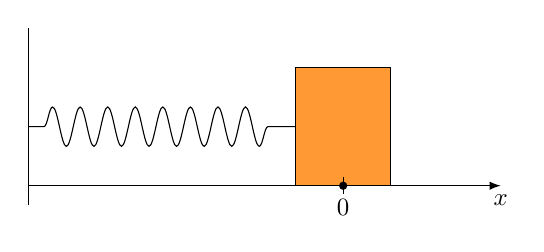
\begin{tikzpicture}[
					spring/.style={ 
					 decoration={
					 snake,
					amplitude=0.25cm, 
					 segment length=3.5mm,
					 post length=2mm,
					 pre length=2mm
					}, 
					decorate 
				}] 
				\draw[-latex] (-4,0)  -- (2,0) node[below] {$x$};
				\draw (-4,-0.25) -- (-4,2); 
				\draw  [draw,fill=orange!80] (-0.6,0) rectangle (0.6,1.5);
				 \draw [spring] (-4,0.75) -- (-0.6,0.75);
				\draw  (0,3pt) -- (0,-3pt);
				 \node [below=2pt] at (0,0) {$0$};
				 \fill (0,0) circle (1.5pt);
			\end{tikzpicture}
		\hfill 
		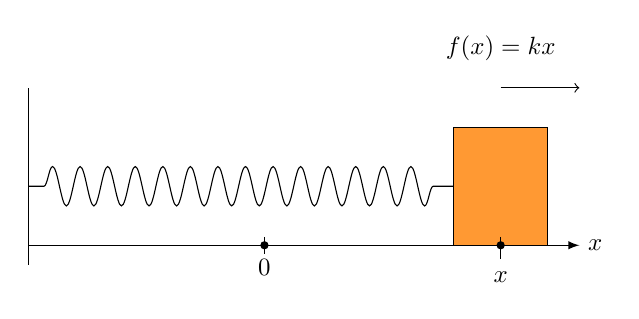
\begin{tikzpicture}[
					spring/.style={ 
					decoration={ 
					snake, 
					 amplitude=0.25cm,
					 segment length=3.5mm,
					post  length=2mm,
					pre length=2mm 
					 },
					decorate 
				 }]
				\draw[-latex] (-5,0) -- (2,0) node [right] {$x$}; 
				\draw  (-5,-0.25) -- (-5,2);
				\draw [draw,fill=orange!80]  (1-0.6,0) rectangle (1+0.6,1.5);
				\draw [spring] (-5,0.75)  -- (1-0.6,0.75);
				 \draw (-2,3pt) -- (-2,-3pt);
				\node [below=2pt]  at (-2,0) {0};
				\fill (-2,0) circle  (1.5pt);
				\draw (1,3pt)  -- (1,-5pt);
				\node [below=7pt] at  (1,0) {$x$};
				\fill (1,0) circle (1.5pt); 
				\node[rectangle,name=node1] at (1,2.5){$f (x)=kx$}; 
				\draw[->] (1,2)--(2,2); 
			\end{tikzpicture}
	\end{center}
	Biết rằng theo định luật Hooke trong Vật lý, khi một chiếc lò xo bị kéo căng thêm $x$ so với độ dài tự nhiên của lò xo thì lò xo trì lại với một lực cho bởi công thức $f(x)=kx$ (N), trong đó $k$  là hệ số đàn hồi của lò xo. Hãy tìm công sinh ra khi kéo lò xo có độ dài từ $15$ cm đến $20$ cm?
	\shortans{3} 
	 \loigiai{
		Khi kéo lò xo từ $10$ cm đến $15$ cm nó bị kéo căng thêm $5$ cm $=  0{,}05$ m.\\
		 Suy ra $f\left(0{,}05\right) = 40 \Leftrightarrow 0{,}05k = 40 \Rightarrow k = 800$ do đó $f(x) = 800x$.\\
		Công được  sinh ra khi kéo căng lò xo từ $15$ cm đến $20$ cm là\\
		$W = \displaystyle\int_{0{,}05}^{0{,}1}{f(x)\mathrm{\,d}x}= \displaystyle\int_{0{,}05}^{0{,}1}{(800x)\mathrm{\,d}x} = 800\left(\dfrac{x^2}{2}\right)\bigg|_{0{,}05}^{0{,}1} = 3$ (J). 
	} 
\end{bt}

% nguồn: Phan2_Lop_12_Dai_so_Chuong_4
\begin{bt}%[2D4H2-6]%[ma:e3502e1c]
	Người thợ hồ nâng một xô nước bị rỉ lên cao $20$ m với tốc độ cố định. Cho trọng lượng của xô là $3$ N, trọng luợng ban đầu của nước là $2$ N. Biết rằng xô nước bị rỉ nên lượng nước trong xô sẽ chảy ra với tốc độ  không đổi trong thời gian nâng xô nước lên. Người ta ước tính rằng lượng nước trong xô sẽ thay đổi theo đồ thị dưới đây. Hỏi người thợ hồ đã dùng một công là bao nhiêu để nâng xô nước lên cao $20$ m, với giả sử rằng bỏ qua trọng lượng sợi dây?
	\begin{center}
		\begin{tikzpicture}[scale=1,>=stealth,font=\footnotesize,line join=round,line cap=round]
				\def\xmin{-1}  \def\xmax{10}
				 \def\ymin{-1} \def\ymax{2}
				\draw[->] (\xmin,0)--(\xmax,0) node [below]{$x$}; 
				\draw[->] (0,\ymin)--(0,\ymax) node  [left]{$y$};
				\node at (0,0)  [below left]{$O$};
				\draw (0,1)  circle (1.5pt) node[left]{$2$};
				\draw  (9,0) circle (1.5pt) node[above]{$20$};
				\draw (0,1)--(9,0); 
				\node[right] at (0,2)  {trọng lượng nước};
				\node[below left]  at (10,0) {độ cao nước};
			\end{tikzpicture}
	\end{center}
	 \shortans{80}
	\loigiai{ 
		Vì trọng lượng của xô là $3$ N không thay đổi nên  công đưa xô lên cao $20$m là
		\[W_{\text{ xô}}= P_{\text{  xô}}\cdot h=3\cdot 20 = 60 \text{ (J)}.\]
		Trọng lượng của nước thay đổi tùy thuộc vào độ cao của xô so với mặt đất. Gọi $x$ là độ cao của xô so với mặt đất, khi đó $f(x)=ax+b$  là trọng lượng của nước tương ứng với độ cao $x$.\\
		 Đồ thị hàm số $f(x)=ax+b$ đi qua $2$ điểm $A(0;2)$ và $B(20;0)$ nên ta có
		\[ 
		 \heva{&a\cdot0 + b = 2\\&a\cdot20 + b=0}\Leftrightarrow
		\heva{&a=-\dfrac{1}{10}\\&  b=2}\Rightarrow
		f(x)=-\dfrac{1}{10}x+2. 
		 \]
		Công sinh ra  khi đưa nước từ mặt đất lên cao $20$ m là
		 \[\displaystyle\int_{0}^{20} f(x) \mathrm{\,d}x=
		\displaystyle\int_{0}^{20} \left(-\dfrac{1}{10}x+2\right) \mathrm{\,d}x= 
		 \left(-\dfrac{1}{20}x^2+2x\right)\Bigg|_{0}^{20}=20 \text{ (J)}.
		\] 
		Vậy công toàn bộ để đưa cả xô và nước lên cao $20$ m là $60+20=80$ J. 
	 }
\end{bt}

% nguồn: Phan2_Lop_12_Dai_so_Chuong_4
\begin{bt}%[2D4H2-6]%[ma:f75f5893]
	Một chiếc xe chuyển động trên đoạn đường thẳng, vận tốc của xe  tại thời điểm $t$ (tính bằng giây) được mô tả bởi hàm số $v(t)=2t^2+3$ (m/s). Tính vận tốc trung bình của xe trong khoảng thời gian từ $t=0$ đến $t=5$ giây (làm tròn đến hàng phần mười).
	\shortans{19,7} 
	\loigiai{ 
		Vận  tốc trung bình của xe trong khoảng thời gian từ $t=0$ đến $t=5$ giây là
		$$v_{\text{ tb}}=\dfrac{1}{b-a}\displaystyle \int_a^b  v(t) \mathrm{\,d}t=\dfrac{1}{5}\displaystyle \int_0^5 (2t^2+3)\mathrm{\,d}t=\dfrac{1}{5}\left(\dfrac{2}{3}t^3+3t\right)\Big|_0^5=\dfrac{1}{5}\left(\dfrac{295}{3}-0\right)=\dfrac{59}{3}\approx 19{,}7.$$
	 }
\end{bt}

% nguồn: Phan2_Lop_12_Dai_so_Chuong_4
\begin{bt}%[2D4H2-6]%[ma:ae5da7c1]
	Một chiếc xe ô tô đang chạy trên đường cao tốc với vận tốc $72$ km/h thì tài xế bất  ngờ đạp phanh làm cho chiếc ô tô chuyển động chậm với gia tốc $a(t)=-\dfrac{8}{5}t$ (m/s$^2$), trong đó $t$ là thời gian tính bằng giây. Hỏi kể từ khi đạp phanh đến khi ô tô dừng hẳn thì ô tô đi chuyển bao nhiêu mét (m)? (Giả sử trên đường ô tô di chuyển không có gì bất thường. Kết quả làm tròn đến hàng phần chục.)
	 \shortans{66,7}
	\loigiai{ 
		Vận tốc của ô tô là  $v(t)=\displaystyle\int{a(t)\mathrm{\,d}t}=\displaystyle\int{\left(-\dfrac{8}{5}t\right)\mathrm{\,d}t}=-\dfrac{4}{5}t^2+C$.\\
		Ta có $72$ km/h $= 20$ m/s. Vì $v(0)=20$ nên $C=20  \Rightarrow v(t)=-\dfrac{4}{5}t^2+20$.\\
		Khi xe dừng hẳn thì vận tốc bằng $0$ nên $-\dfrac{4}{5}t^2+20=0 \Rightarrow t=5$.\\ 
		Quãng đường cần  tìm là $S=\displaystyle\int_{0}^{5}{\left(-\dfrac{4}{5}t^2+20\right)\mathrm{\,d}t}=\left(-\dfrac{4}{15}t^3+20t\right)\bigg|_{0}^{5}=\dfrac{200}{3}$ m.
	 }
\end{bt}

% nguồn: Phan2_Lop_12_Dai_so_Chuong_4
\begin{bt}%[2D4H2-6]%[ma:c439d3d2]
	Nhằm tri ân người dân địa phương đã luôn tin tưởng, đồng hành với doanh nghiệp. Tập đoàn NXS đã tổ chức ngày hội cảm ơn vào ngày 10/07/2024. Trong chuỗi sự kiện đặc biệt này, tất cả người dân địa phương đều được miễn phí vé vào cổng, thỏa  thích tận hưởng các trò chơi, tham quan các công trình kỳ thú, ấn tượng tại $05$ công viên chủ đề được đầu tư, xây dựng hoành tráng với hàng trăm tiện ích. Gọi $B(t)$ là hàm số biểu thị số lượng khách tham quan sau $t$ giờ mở cửa. Khi đó tốc độ thay đổi lượng khách tham quan trong ngày được biểu diễn bằng hàm số $B'(t)=4t^3-3t^2+200$, trong đó $t$ tính bằng giờ ($0\le t\le 8$), $B'(t)$ tính bằng khách/giờ. Sau $2$ giờ đã có $1\,200$ người có mặt. Hỏi sau $6$ giờ lượng khách tham quan là bao nhiêu người?
	\shortans{3072} 
	 \loigiai{
		 Ta có
		 \[B(t)=\displaystyle\int B'(t)\mathrm{\,d}t=t^4-t^3+200t+C,\,C\in \mathbb{R}\Rightarrow B\left( 2 \right)=1\,200\Rightarrow C=792.\]
		 Suy ra $B(t)=t^4-t^3+200t+792$.\\
		Sau $6$  giờ lượng khách tham quan là $B(6)=3\,072$ (người).
	 }
\end{bt}

% nguồn: Phan2_Lop_12_Dai_so_Chuong_4
\begin{bt}%[2D4H2-6]%[ma:096fe2a2]
	Chủ một trung tâm thương mại muốn cho thuê một số gian hàng như nhau. Người đó muốn cho thuê mỗi gian  hàng với giá là $x$ triệu đồng $(x>0)$. Khi đó doanh thu của cửa hàng được biểu diễn theo hàm số $T(x)$. Tốc độ thay đổi doanh thu từ các gian hàng đó được biểu diễn bởi hàm số $T'(x)=-10x+200$, trong đó $T'(x)$ tính bằng triệu đồng. Biết rằng nếu giá thuê cho mỗi gian hàng là $10$ triệu đồng thì doanh thu là $1\,800$ triệu đồng. Tìm giá trị của $x$ để người đó có doanh thu là cao nhất?
	 \shortans{20}
	 \loigiai{
		 Ta có
		\[T(x)=\displaystyle\int T'(x)\mathrm{\,d}x=\displaystyle\int  (-10x+200)\mathrm{\,d}x=-5x^2+200x+C,\,C\in \mathbb{R}.\]
		Khi giá cho thuê mỗi gian hàng là $10$ triệu đồng thì doanh thu là  $1\,800$ triệu đồng nên ta có
		\[T(10)=1\,800\Rightarrow C=300.\] 
		Do đó $T(x)=-5x^2+200x+300=-5(x-20)^2+2\,300\le 2\,300$, dấu \lq\lq =\rq\rq~ xảy ra khi  $x=20$.\\
		Suy ra doanh thu cao nhất mà chủ trung tâm thương mại có thể thu về là $2\,300$ triệu đồng và khi  đó mỗi gian hàng có giá cho thuê là $20$ triệu đồng.\\
		Vậy $x=20$  (triệu đồng).
	 }
\end{bt}

% nguồn: Phan2_Lop_12_Dai_so_Chuong_4
\begin{bt}%[2D4H2-6]%[ma:28c5a639]
	Một bác thợ xây bơm nước vào bể chứa nước. Gọi $h(t)$ là thể tích nước bơm được sau $t$ giây. Cho $h'(t)=6at^2+2bt$ và ban  đầu bể không có nước. Sau $3$ giây thì thể tích nước trong bể là $90$ m$^3$ và sau $6$ giây thì thể tích nước trong bể là $504$ m$^3$. Tính thể tích của lượng nước trong bể sau khi bơm được $9$ giây.
	 \shortans{1458}
	 \loigiai{
		Ta có $\displaystyle\int_{0}^{3}{(6at^2+2bt)\mathrm{\,d}t}=90 \Leftrightarrow (2at^3+bt^2)\bigg|_{0}^{3}=90 \Leftrightarrow  54a+9b=90$. (1)\\
		Mặt khác $\displaystyle\int_{0}^{6}{(6at^2+2bt)\mathrm{\,d}t}=504 \Leftrightarrow  (2at^3+bt^2)\bigg|_{0}^{6}=504 \Leftrightarrow 432a+36b=504$. (2)\\
		Từ $(1)$ và $(2)$ $\Rightarrow \begin{cases} a=\dfrac{2}{3}\\ b=6
	\end{cases}$ nên sau khi bơm $9$ giây thì thể tích nước trong bể là\\
	 $V=\displaystyle\int_{0}^{9}{(4t^2+12t)\mathrm{\,d}t}=\left(\dfrac{4}{3}t^3+6t^2\right)\bigg|_{0}^{9}=1458$ (m$^3$).
} 
\end{bt}

% nguồn: Phan2_Lop_12_Dai_so_Chuong_4
\begin{bt}%[2D4H2-6]%[ma:6408840f]
	Tốc độ tăng trưởng chiều cao sau khi trồng (đơn vị: centimet/năm) của một loài cây lấy gỗ ở năm thứ $t$ được  cho bởi hàm số $h'(t)=\log_{1{,}2}\big(20t+1\big)+30$.
	Từ năm thứ $20$ đến năm thứ $30$ sau khi trồng, cây cao thêm được bao nhiêu mét (\textit{làm  tròn kết quả đến hàng phần trăm})?
	 \shortans{6,41}
	\loigiai{ 
		Từ năm thứ $20$ đến năm  thứ $30$ sau khi trồng, cây cao thêm được
		 \[
		\displaystyle\int_{20}^{30}\Big[\log_{1{,}2}(20t+1)+30\Big]\mathrm{\,d}t \approx 640{,}6 \text{ cm} \approx 6{,}41  \text{ m}.
		\] 
	 }
\end{bt}

% nguồn: Phan2_Lop_12_Dai_so_Chuong_4
\begin{bt}%[2D4H2-6]%[ma:3a5bb2e7]
	Một ô tô đang chuyển động thẳng đều trên cao tốc với vận tốc $28$ (m/s) thì người lái đạp phanh. Từ thời điểm đạp phanh đó, ô tô chuyển động chậm dần đều với vận tốc $v(t)=-4t+28$ (m/s), trong đó $t$  là khoảng thời gian tính bằng giây kể từ lúc bắt đầu đạp phanh. Hỏi từ lúc đạp phanh đến khi ô tô dừng hẳn, ô tô di chuyển được bao nhiêu mét nữa?
	 \shortans{98}
	 \loigiai{
		Khi ô tô dừng  hẳn thì $v(t)=0\Leftrightarrow -4t+28=0\Leftrightarrow t=7$ (s).\\
		Quãng đường  ô tô đi đường kể từ lúc đạp phanh đến khi dừng hẳn là
		\begin{center}
			$\displaystyle \int_{0}^{7}\left( -4t+28\right)\mathrm{\,d}t=98$ (m). 
		\end{center}
	} 
\end{bt}

% nguồn: Phan2_Lop_12_Dai_so_Chuong_4
\begin{bt}%[2D4H2-6]%[ma:c9bd00af]
	Một vật chuyển động dọc theo một đường thẳng sao cho vận tốc của nó tại thời điểm $t$ (giây) là $v(t)=t^2-t-6$ (mét/giây). Quãng đường (mét) vật đi được trong khoảng thời gian $1 \le t \le 4$  bằng (làm tròn tới hàng phần chục)
	\shortans{10,2} 
	\loigiai{ 
		Gọi  $S$ là quãng đường vật đi được trong khoảng thời gian $1 \le t \le 4$.\\
		Ta có  $S=\displaystyle\int_{1}^{4}{|v(t)|\mathrm{\,d}t}=\displaystyle\int_{1}^{4}{|t^2-t-6|\mathrm{\,d}t}=\displaystyle\int_{1}^{3}{|t^2-t-6|\mathrm{\,d}t}+\displaystyle\int_{3}^{4}{|t^2-t-6|\mathrm{\,d}t}$\\
		$=-\dfrac{22}{3}+\left|\dfrac{17}{6}\right|=\dfrac{61}{6} \approx 10{,}2$ m. 
	} 
\end{bt}

% nguồn: Phan2_Lop_12_Dai_so_Chuong_4
\begin{bt}%[2D4H2-6]%[ma:9331064c]
	Tốc độ tăng trưởng của một đàn gấu mèo tại thời điểm $t$ tháng kể từ khi người ta  thả $100$ cá thể đầu tiên vào một khu rừng được ước lượng bởi công thức $P'(t)=8t+30$ (con/tháng), với $P(t)$ là số lượng cá thể trong đàn tại thời điểm $t$ tháng tương ứng (nguồn: Chris Kirkpatrick, Barbara Alldred, Crystal Chilvers, Beverly Farahani, Kristina Farentino, Angelo Lillo, Ian Macpherson, John Rodger, Susanne Trew, Advanced Function, Nelson 2012). Dựa vào tốc độ tăng trưởng đã cho, hãy ước tính số cá thể của đàn gấu mèo này tại thời điểm $3$ tháng kể từ khi chúng được thả vào rừng.
	\shortans{226} 
	\loigiai{ 
		Ta có  \[P(t)=\displaystyle\int P'(t)\mathrm{\,d}t=\displaystyle\int (8t+30)\mathrm{\,d}t=4t^2+30t+C.\]
		Lại có ban đầu người ta thả  $100$ cá thể gấu mèo nên
		 \[P(0)=100\Rightarrow C=100\Rightarrow P(t)=4t^2+30t+100.\]
		Vậy số cá thể của đàn gấu mèo này tại thời điểm $3$  tháng kể từ khi chúng được thả vào rừng là
		\[P(3)=4\cdot 3^2+30\cdot  3+100=226~(\text{cá thể}).\]
	 }
\end{bt}

% nguồn: Phan2_Lop_12_Dai_so_Chuong_4
\begin{bt}%[2D4H2-6]%[ma:783e8245]
	Hai công ty, công ty A và công ty B, cùng ra mắt sản phẩm cạnh tranh thị trường mới vào cùng thời điểm. Thị phần  được đo bằng số lượng khách hàng lũy kế.\\
	Công ty A: Bắt  đầu với $0$ khách hàng. Trong giai đoạn đầu, chiến dịch marketing hiệu quả giúp tốc độ thu hút khách hàng mới của họ tăng dần theo thời gian, được mô tả bởi hàm $f(t) = 2t + 7$ (nghìn khách hàng/tháng), với $t$ là số tháng kể từ khi ra mắt. \\
	Công ty B: Nhờ có uy tín từ trước, họ bắt đầu với $10$ nghìn khách hàng đặt trước sản phẩm. Sau đó, họ duy trì một tốc độ thu hút khách hàng mới ổn định  là $10$ nghìn khách hàng/tháng.\\
	Hỏi sau khoảng bao nhiêu tháng kể từ khi ra mắt, tổng số lượng khách hàng lũy kế  của công ty A bằng tổng số lượng khách hàng lũy kế của công ty B (tính cả $10$ nghìn khách hàng ban đầu)?
	 \shortans{5}
	\loigiai{ 
		Số lượng khách hàng lũy kế của công  ty A sau $t$ tháng là \[S_A(t) = \displaystyle\int_{0}^{t} (2x+7) \, \mathrm{d}x =(x^2+7x)\bigg|_{0}^{t} = t^2+7t\quad (\text{nghìn khách hàng}).\]
		Số lượng khách hàng lũy kế của công ty B sau $t$ tháng là \[S_B(t) = 10 + \displaystyle\int_{0}^{t} 10  \, \mathrm{d}x = 10 + (10x)\bigg|_{0}^{t} = 10 + 10t\quad (\text{nghìn khách hàng}).\]
		Theo giả thiết, ta có $S_A(t)  = S_B(t)$.\\
		Suy ra 
		 \allowdisplaybreaks
		\begin{eqnarray*}
			 &&t^2+7t = 10+10t\\
			&\Leftrightarrow &t^2  - 3t - 10 = 0\\
			&\Leftrightarrow  &\hoac{&t=5&(\text{nhận})\\&t=-2&(\text{loại}).}
		\end{eqnarray*}
	 }
\end{bt}

% nguồn: Phan2_Lop_12_Dai_so_Chuong_4
\begin{bt}%[2D4H2-6]%[ma:5213fed8]
	 Một xe mô tô đang chạy với vận tốc $20$ m/s thì tài xế giảm ga và kéo phanh. Từ thời điểm đó, xe chuyển động chậm dần đều với vận tốc được mô tả bởi phương trình: $v(t)=-4t+20$ (m/s), trong đó thời gian $t$ được tính bằng giây. Hỏi từ lúc giảm ga và kéo phanh đến khi dừng hẳn, mô tô di chuyển được quảng đường bao nhiêu mét?
	 \shortans{50}
	\loigiai{ 
		Vận tốc  ban đầu là $20$ m/s. Xét $v(t)=20\Leftrightarrow -4t+2-=20\Leftrightarrow t=0$ (giây).\\
		Do đó thời điểm kéo phanh là thời điểm  $t=0$ (giây).\\
		Khi dừng hẳn vận tốc là $0$ m/s.  Xét $v(t)=0\Leftrightarrow -3t+20=0\Leftrightarrow t=5$ (giây).\\
		Do đó thời điểm xe dừng hẳn là thời điểm $t=0$ (giây).\\ 
		 Vậy quãng đường cần tìm là $S=\displaystyle\int_{0}^{5}v(t)\mathrm{\,d}t=\displaystyle\int_{0}^{5}(-4t+20)\mathrm{\,d}t=\left(-2t^2+20t\right)\bigg|_0^5=50$.
	} 
\end{bt}

% nguồn: Phan2_Lop_12_Dai_so_Chuong_4
\begin{bt}%[2D4H2-6]%[ma:75b4e15e]
	Một phần bề mặt phía trên của các gợn sóng nước biển có hình dạng đồ thị hàm số bậc ba khi gắn hệ trục toạ độ $Oxy$. Biết rằng đồ thị hàm số bậc ba có các điểm  cực trị lần lượt là $M(-2;1)$ và $N(0;1{,}2)$, đơn vị trên hệ trục toạ độ là mét.
	Hai vị trí $A$ và $B$ có hoành độ lần lượt là $-3$ và $1$ nằm trên đường cong của các  gợn sóng đó.
	Tính độ dài đường cong $AB$ (\textit{làm tròn kết quả đến hàng phần trăm}). Biết rằng độ dài đường cong có phương trình $y=f(x)$ từ  điểm $C\big(c;f(c)\big)$ tới điểm $D\big(d;f(d)\big)$ với $c<d$ được tính bởi công thức $l_{AB} = \displaystyle\int_{c}^{d} \sqrt{1 + \big(f'(x)\big)^2}\mathrm{\,d}x$.
	\shortans{4,07} 
	 \loigiai{
		 Gọi hàm số bậc ba là $y=f(x)=ax^3+bx^2+cx+d$ có $f'(x)=3ax^2+2bx+c$.\\
		Do $M(-2;1)$ và $N(0;1{,}2)$ là hai  điểm cực trị nên
		$\heva{&f'(-2)=0\\ &f'(0)=0  \\ &f(-2)=1\\ &f(0)=1{,}2.}$\\
		Thay  vào, ta được $a=-0{,}05$; $b=-0{,}15$; $c=0$; $d=1{,}2$ nên $f'(x)=-0{,}15x^2-0{,}3x$.\\
		Vậy độ dài đường  cong $AB$ là
		 \[
		l_{AB} = \displaystyle\int_{-3}^{1} \sqrt{1 + \left(-0{,}15x^2 - 0{,}3x\right)^2}\mathrm{\,d}x \approx 4{,}07 \text{  (mét)}.
		 \]
	 }
\end{bt}

% nguồn: Phan2_Lop_12_Dai_so_Chuong_4
\begin{bt}%[2D4H2-6]%[ma:d14462a8]
	Cho đồ thị biểu diễn vận tốc của hai xe A và B khởi hành cùng một lúc và cùng vạch xuất phát, đi cùng chiều  trên một con đường. Biết đồ thị biểu diễn vận tốc của xe A là một đường parabol và đồ thị biểu diễn vận tốc của xe B là một đường thẳng như hình vẽ bên. Hỏi sau $5$ giây kể từ lúc xuất phát thì khoảng cách giữa hai xe là bao nhiêu mét, biết rằng xe $A$ sẽ dừng lại khi vận tốc bằng $0$ (kết quả làm tròn đến hàng phần chục)?
	\begin{center}
		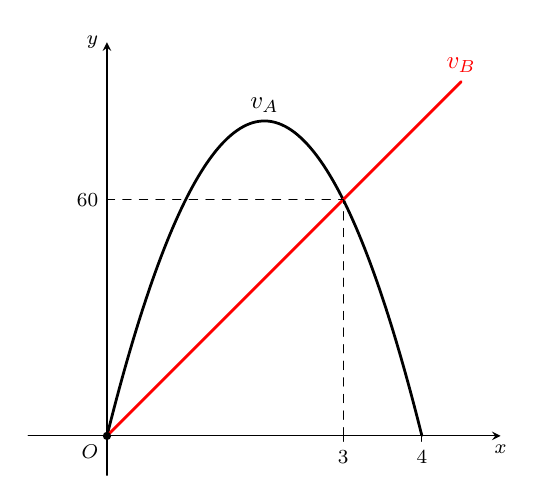
\begin{tikzpicture}[line cap=round,line join=round,>=stealth,x=1.0cm,y=1.0cm]
				\draw[->,color=black] (-1,0.) -- (5,0.) node[below] {\footnotesize  $x$};
				\foreach  \x in {3,4}
				\draw[shift={(\x,0)},color=black] (0pt,2pt) -- (0pt,-2pt)  node[below] {\footnotesize $\x$};
				\draw[->,color=black] (0,-0.5) --  (0,5) node[left] {\footnotesize $y$};
				\draw (0,0) node[below left] {\footnotesize  $O$}
					(0,3)  node[left] {\footnotesize $60$};
				\draw[line width=1pt,smooth,samples=100,domain=0:4] plot (\x,{(\x)*(4-(\x))}); 
				\draw[color=red,line width=1pt,smooth,samples=100,domain=0:4.5] plot (\x,{(\x)})  node[above]{$v_B$};
				\draw (2,4)  node[above]{$v_A$};
				\draw[dashed] (3,0)--(3,3)--(0,3); 
				\fill  (0cm,0cm) circle (1.5pt);
			\end{tikzpicture}
	\end{center}
	 \shortans{36,7}
	\loigiai{ 
		Đồ thị biểu diễn vận tốc của xe A là $(P)$ có phương  trình $v_A=at^2+bt+c~(a\ne 0)$ đi qua điểm $(0;0);\,(3;60);\,(4;0)\Rightarrow v_A=-20t^2+80t$.\\
		Đồ thị biểu diễn vận tốc của xe  B là đường thẳng $\Delta$ có phương trình $v_B=mt+n~(m\ne 0)$ đi qua điểm $(0;0);\,(3;60)\Rightarrow v_B=20t$.\\
		 Ta có $v_A=-20t^2+80t=0 \Rightarrow t=4$ nên xe A dừng lại sau giây thứ $4$.\\
		Do  đó quãng đường xe A đi được sau $4$ giây là
		\[S_A=\displaystyle\int_0^4 \left(-20t^2+80t  \right)\mathrm{\,d}t=\dfrac{640}{3}~(\text{m}).\]
		Quãng đường xe B đi được sau $5$  giây đầu là
		 \[S_B=\displaystyle\int_0^5 20t\mathrm{\,d}t=250~( \text{ m}).\]
		Khoảng cách giữa hai xe sau $5$ giây kể từ  lúc xuất phát là
		\[\Delta  S=\left|S_A-S_B\right|=\dfrac{110}{3}=36{,}7~(\text{m}).\]
	 }
\end{bt}

% nguồn: Phan2_Lop_12_Dai_so_Chuong_4
\begin{bt}%[2D4H2-6]%[ma:93151ca1]
	Một ô  tô đang chạy với vận tốc $12$ m/s thì người lái xe đạp phanh.
	Từ thời điểm đó, ô tô chuyển động chậm dần đều với vận tốc $v(t)=-2t+12$ (m/s), trong đó $t$ là khoảng thời gian  được tính bằng giây, kể từ lúc bắt đầu đạp phanh.
	Quãng  đường ô tô di chuyển được trong $10$ giây cuối cùng bằng bao nhiêu (\textit{làm tròn kết quả đến hàng đơn vị})?
	 \shortans{84}
	\loigiai{ 
		Khi ô tô dừng  hẳn thì $v(t)=0 \Leftrightarrow -2t+12=0 \Leftrightarrow t=6$ (s).\\
		Do đó, trong $10$  giây cuối cùng thì có $4$ giây ô tô chuyển động với vận tốc $12\,\mathrm{m/s}$ và $6$ giây cuối cùng ô tô chuyển động chậm dần đều với vận tốc $v(t)=-2t+12$ (m/s).\\
		Vậy quãng đường ô tô di chuyển được trong $10$ giây cuối cùng  bằng
		\[ 
		S = 4.12  + \displaystyle\int_{0}^{6} (-2t+12)\mathrm{\,d}t = 48 + 36 = 84\text{ (m)}.
		 \]
	 }
\end{bt}

% nguồn: Phan2_Lop_12_Dai_so_Chuong_4
\begin{bt}%[2D4H2-6]%[ma:c4b08c37]
	 \immini[thm]
	{Hiệu suất của tim là lưu lượng máu được bơm bởi tim trên một đơn vị thời gian (lưu lượng máu chảy vào động mạch chủ). Để đo hiệu suất của tim, người ta bơm $A$ (mg) chất chỉ thị màu vào tâm  nhĩ phải, chảy qua tim rồi vào động mạch chủ và đo nồng độ chất chỉ thị màu còn lại ở tim đến thời điểm $T$ (s) khi chất chỉ thị màu tan sạch. Gọi $c(t)$ là nồng độ (mg/l) chất chỉ thị màu tại thời điểm $t$ (s) thì hiệu suất của tim được xác định bởi}
	{\definecolor{c0293e1}{RGB}{2,147,225} 
	\definecolor{cdd1b02}{RGB}{221,27,2} 
	\definecolor{cfc5f54}{RGB}{252,95,84} 
	\definecolor{cc97901}{RGB}{201,121,1} 
	\definecolor{cc00602}{RGB}{192,6,2} 
	\definecolor{c700902}{RGB}{112,9,2} 
	 \definecolor{c156295}{RGB}{21,98,149}
	 \definecolor{c225d6a}{RGB}{34,93,106}
	 \definecolor{cc21d02}{RGB}{194,29,2}
	\definecolor{c235d6b}{RGB}{35,93,107} 
	\begin{tikzpicture}[line cap=round,line join=round,scale=0.5]
			\begin{scope}[cm={0.42,-0,-0,0.42,(0.04,17.68)}]
				\path[draw,fill=c0293e1,even odd rule,line cap=round,line width=0.1cm,miter limit=4]  (7.33,8.51).. controls +(168:0.1) and +(-82:0.1)..
					(7.11,8.81).. controls +(96:0.2) and  +(-90:0.7)..
					(7.03,11.11).. controls +(90:0.5)  and +(-105:0.2)..
					(7.08,11.9).. controls  +(75:0.5) and +(168:0.4)..
					(7.85,12.51).. controls  +(-14:0.3) and +(139:0.5)..
					(8.95,11.83) -- (9.07,11.72) --  (9.04,11.19).. controls +(-94:1.1) and +(77:0.4)..
					(8.76,8.97).. controls +(-101:0.2) and  +(42:0.1)..
					(8.61,8.68)..  controls +(-135:0.1) and +(18:0.1)..
					 (8.39,8.54).. controls +(-165:0.1) and +(-14:0.1)..
					 (7.33,8.51) -- cycle;
				\path[draw,fill=c0293e1,even odd rule,line cap=round,line width=0.09cm,miter limit=4]  (11.96,17.81).. controls +(147:0.8) and +(-37:1.1)..
					(9.95,19.25) -- (8.86,20.09)  -- (8.57,20.09).. controls +(180:0.7) and +(14:0.2)..
					(6.92,19.98) -- (6.73,19.92) -- (6.6,20.01).. controls +(144:0.2) and +(-87:0.2).. 
					(6.3,20.51).. controls  +(96:0.1) and +(180:0)..
					(6.31,20.68).. controls  +(0:0.1) and +(-124:0)..
					(7.08,20.84).. controls +(40:0.1)  and +(-30:0.3)..
					 (6.82,21.11).. controls +(150:0.3) and +(-90:0.1)..
					 (6.51,21.42).. controls +(90:0.2) and +(-144:0.2)..
					(6.74,21.84) -- (6.87,21.93) -- (7.83,21.62).. controls  +(-18:2.3) and +(172:1)..
					(11.79,20.57).. controls +(-7:0.5) and  +(-173:0.4)..
					(13.59,20.55)..  controls +(8:0.7) and +(-153:0.7)..
					(15.39,21.17).. controls +(27:0.5) and +(130:0.3).. 
					(16.08,21.21).. controls +(-52:0.1) and  +(90:0.2)..
					(16.16,20.92) --  (16.16,20.74) -- (15.92,20.61).. controls +(-152:0.3) and +(90:0.1)..
					(15.54,20.32).. controls +(-90:0) and +(153:0.2).. 
					(15.87,20.14).. controls  +(-25:0.3) and +(90:0.1)..
					(16.19,19.9).. controls +(-90:0.2) and  +(28:0.3)..
					(15.6,19.15).. controls +(-153:0.1) and +(28:0.3).. 
					(15.32,20.02)..  controls +(-154:0.7) and +(65:0.9)..
					(13.12,18.89).. controls +(-117:0.4) and +(90:0.5).. 
					(12.89,17.67)..  controls +(-90:0.2) and +(0:0)..
					(12.88,17.22).. controls +(0:0)  and +(-32:0.6)..
					(11.96,17.81)  -- cycle;
				\path[draw,even odd rule,line  cap=round,line width=0.09cm,miter limit=4] (7,18.06).. controls +(87:1.1) and +(-96:0.8)..
					 (7.17,20.01) -- (7.23,20.67) -- (7.39,20.83).. controls +(46:0.6) and +(159:0.7)..
					(8.92,21.05) -- (9.17,20.96) -- (9.12,19.26)  -- cycle;
				\path[draw,fill=c0293e1,even odd rule,line cap=round,line width=0.1cm,miter limit=4] (7.07,18.26).. controls +(90:0.1)  and +(-96:0.8)..
					(7.21,19.87)  -- (7.29,20.64) -- (7.44,20.79).. controls +(45:0.1) and +(-151:0.1)..
					(7.78,21.04)..  controls +(25:0.2) and +(180:0.2)..
					(8.24,21.13).. controls +(-2:0.2) and  +(162:0.3)..
					(8.79,21.03) --  (9.08,20.93) -- (9.09,20.77).. controls +(-90:0.1) and +(88:0.4)..
					(9.08,19.96) -- (9.06,19.3) -- (8.08,18.75)..  controls +(-150:0.6) and +(45:0)..
					(7.09,18.18)..  controls +(180:0) and +(-90:0.1)..
					(7.07,18.26)  -- cycle;
				 \path[draw,even odd rule,line cap=butt,line join=miter,line width=0.09cm,miter limit=4] (7.44,18.85).. controls +(19:0.5) and +(-120:0.5)..
					 (8.5,19.73).. controls +(62:0.4) and +(-171:0.3)..
					(9.24,20.25) -- (10.03,20.35).. controls  +(-2:0.4) and +(112:0.2)..
					(10.61,19.93) -- (11.07,18.85).. controls +(-59:1.1) and  +(161:0.7)..
					 (12.96,17.41).. controls +(-51:4.7) and +(72:2.1)..
					(14.19,9.83).. controls +(-124:0.7) and +(42:2.5).. 
					(12.75,7.92).. controls +(173:1.8)  and +(-50:2)..
					(8.09,10.3).. controls  +(124:1.6) and +(-79:3)..
					(5.43,14.74).. controls  +(94:2) and +(-150:1.6)..
					(7.44,18.85) -- cycle; 
				\path[draw,fill=cdd1b02,even odd rule,line cap=round,line width=0.1cm,miter limit=4] (12.61,7.99).. controls +(172:0.3) and  +(-15:0.3)..
					(11.31,8.27)..  controls +(164:1.4) and +(-53:1.3)..
					(8.04,10.46).. controls +(127:0.2) and  +(-46:0.4)..
					 (7.37,11.22).. controls +(134:1.1) and +(-63:0.6)..
					(6.1,12.84).. controls +(117:0.7) and  +(-87:0.6)..
					 (5.48,14.96).. controls +(93:0.9) and +(-123:0.8)..
					(6.14,17.58).. controls +(56:0.6) and  +(-158:0.5)..
					(7.62,18.86)..  controls +(22:0.2) and +(-133:0.2)..
					(8.28,19.32)..  controls +(45:0.1) and +(-125:0.2)..
					(8.54,19.67)..  controls +(58:0.5) and +(-173:0.8)..
					(9.68,20.25).. controls +(6:0.4) and  +(162:0.1)..
					(10.24,20.25).. controls  +(-21:0.1) and +(129:0.1)..
					(10.44,20.11).. controls  +(-51:0.1) and +(113:0.4)..
					 (10.77,19.41).. controls +(-67:0.7) and +(128:0.4)..
					(11.34,18.37).. controls +(-51:0.3)  and +(146:0.3)..
					(11.95,17.81).. controls +(-33:0.2) and +(161:0.2).. 
					 (12.79,17.4).. controls +(-14:0.1) and +(126:0.5)..
					(13.22,16.96).. controls  +(-53:2.2) and +(82:1.5)..
					 (14.84,12.3).. controls +(-98:0.4) and +(73:0.4)..
					(14.58,11.16).. controls +(-108:0.5)  and +(62:0.1)..
					(14.09,9.79).. controls +(-113:0.1) and  +(84:0.1)..
					(14,9.48)..  controls +(-99:0.1) and +(54:0.1)..
					(13.86,9.14).. controls +(-124:0.2)  and +(-14:0)..
					 (12.72,7.98).. controls +(180:0) and +(-11:0.1)..
					(12.61,7.99)  -- cycle;
				\path[draw,fill=cdd1b02,even odd rule,line cap=round,line  width=0.1cm,miter limit=4] (12.73,20.52).. controls +(110:1.6) and +(0:0)..
					(11.43,18.23).. controls +(-172:0.2) and +(6:0.3).. 
					 (10.12,20.27).. controls +(-176:0.2) and +(0:0)..
					(9.42,20.24).. controls +(180:0)  and +(-108:0.2)..
					(9.48,20.7).. controls +(72:0.5) and +(-132:0.8).. 
					(10.25,22.07).. controls +(48:0.1)  and +(-90:0.1)..
					(10.39,22.37).. controls +(90:0.1) and +(-55:0.4).. 
					(10.04,23.02).. controls +(123:0.2) and  +(-90:0)..
					(9.88,23.31).. controls  +(90:0.1) and +(-153:0.1)..
					(10.12,23.58).. controls  +(22:0.1) and +(180:0.1)..
					 (10.32,23.62).. controls +(0:0.1) and +(105:0.2)..
					 (10.48,23.4).. controls +(-72:0.3) and +(-157:0.2)..
					(10.75,23.17).. controls +(23:0.1)  and +(-115:0.2)..
					(10.93,23.41).. controls  +(63:0.2) and +(-160:0.1)..
					(11.15,23.66).. controls +(24:0.1) and +(140:0.1).. 
					(11.34,23.66)..  controls +(-27:0.1) and +(59:0.1)..
					(11.45,23.38).. controls +(-117:0) and +(52:0.2).. 
					(11.25,23.11).. controls  +(-129:0.3) and +(90:0.1)..
					(11.07,22.75).. controls +(-90:0.1) and +(130:0.1).. 
					(11.14,22.54).. controls +(-49:0.1) and +(-178:0.3).. 
					(11.51,22.47).. controls +(0:0.3) and  +(-130:0.1)..
					 (11.85,22.54).. controls +(52:0.2) and +(-111:0.3)..
					 (12.16,23.13).. controls +(69:0.3) and +(180:0.2)..
					(12.58,23.49)..  controls +(-3:0.2) and +(142:0.2)..
					(12.99,23.33) -- (13.06,23.26) -- (13.01,22.89).. controls +(-98:0.4)  and +(110:0.1)..
					 (13,22.4).. controls +(-69:0.2) and +(180:0.1)..
					(13.3,22.11).. controls +(0:0.2)  and +(-124:0.4)..
					 (13.77,22.5) -- (13.97,22.79) -- (14.13,22.78).. controls +(-6:0.2) and +(113:0.1)..
					(14.51,22.57).. controls +(-69:0.1)  and +(62:0.4)..
					(14.35,22.13).. controls +(-120:0.2)  and +(82:0.1)..
					(14.12,21.66)..  controls +(-84:0.6) and +(103:0.4)..
					(14.8,20.83).. controls  +(-155:0.4) and +(-14:0.7)..
					 (12.73,20.52) -- cycle;
				\path[draw,fill=cdd1b02,even odd rule,line cap=round,line  width=0.1cm,miter limit=4] (13.48,18.58).. controls +(170:0.1) and +(-27:0.1)..
					 (13.26,18.66) -- (13.15,18.71) -- (13.04,19.36) -- (14.87,19.86) -- (14.87,19.22) -- (14.76,19.14).. controls +(-141:0.3) and +(25:0.1)..
					(14.01,18.63)..  controls +(-162:0.2) and +(-16:0.1)..
					(13.48,18.58)  -- cycle;
				\path[draw,fill=cfc5f54,even odd rule,line cap=butt,line join=miter,line width=0.03cm] (11.89,15.62).. controls +(-44:0.5)  and +(93:1.4)..
					(12.82,13.73).. controls +(-85:0.6) and  +(58:0.5)..
					(12.45,12.27)..  controls +(-65:1.1) and +(80:1.5)..
					(12.82,8.52).. controls +(138:1.2) and +(-67:1.2).. 
					(10.76,11.51).. controls +(97:0.6) and +(-153:0.6).. 
					(11.29,12.96).. controls +(164:0.7) and  +(-76:0.5)..
					 (10.56,14.29).. controls +(74:0.9) and +(-159:0.6)..
					 (11.89,15.62) -- cycle;
				\path[draw,fill=cfc5f54,even odd rule,line cap=butt,line join=miter,line width=0.03cm] (7.46,18.32)..  controls +(-152:2) and +(81:1.2)..
					(5.64,14.89).. controls +(47:1.8) and  +(174:0.6)..
					(8.26,16.39).. controls  +(34:1.3) and +(-126:0.7)..
					(10.04,18.16).. controls +(146:0.6) and +(31:2.9).. 
					(7.46,18.32) -- cycle; 
				\path[draw,fill=cc97901,even  odd rule,line cap=butt,line join=miter,line width=0.09cm,miter limit=4] (10.73,19.47).. controls +(-60:0.4) and +(76:0.4)..
					(11.07,18.42).. controls +(-97:0.6) and +(49:0.4).. 
					(10.38,17.25).. controls +(-154:0.3) and +(33:0.3).. 
					 (9.6,16.8).. controls +(-161:0.3) and +(40:0.3)..
					(8.87,16.39) -- (8.22,16.21) -- (7.68,15.95)  -- (7.22,15.74) -- (7.4,15.66) -- (7.96,16) -- (7.99,15.87) -- (8.41,16.13) -- (8.66,16.21) -- (7.76,15.16).. controls +(-137:0.2) and +(86:0.1)..
					(7.46,14.75).. controls +(-167:0.2) and  +(50:0.2)..
					 (7.02,14.28) -- (6.41,13.75).. controls +(21:0.2) and +(93:0.2)..
					(6.78,13.78) -- (6.71,13.56) -- (6.63,13.23) -- (6.63,13.09) -- (6.54,12.74) -- (6.66,12.88) --  (6.72,13.06).. controls +(99:0.1) and +(166:0.1)..
					(6.95,13.11) -- (6.85,13.33) -- (6.98,13.92).. controls +(65:0.4) and  +(172:0.2)..
					(7.49,14.47).. controls  +(-72:0.3) and +(63:0.3)..
					(7.41,13.65).. controls +(-114:0.8) and +(73:0.6).. 
					(6.86,11.89)..  controls +(-114:0.3) and +(126:0.1)..
					(6.96,11.43).. controls +(-83:0.1)  and +(-127:0.1)..
					(7.09,11.47).. controls +(101:0.4)  and +(-122:0.3)..
					(7.32,12.49).. controls +(73:0.1)  and +(141:0.4)..
					(7.61,12.51)  -- (8.95,10.95).. controls +(-63:0.4) and +(157:0.5)..
					(9.88,9.98)..  controls +(-31:0.2) and +(128:0.3)..
					(10.43,9.47) --  (10.79,8.85).. controls +(-61:0.4) and +(129:0.2)..
					 (11.21,8.32).. controls +(126:0.4) and +(151:0.4)..
					(11.26,8.62) --  (10.94,8.88) -- (10.63,9.38).. controls +(90:0.1) and +(139:0.3)..
					(10.77,9.45).. controls  +(-28:0.5) and +(121:0.4)..
					(11.61,8.55)..  controls +(-39:1.3) and +(162:0.2)..
					(12.57,8).. controls +(149:0.4) and +(-61:0.5).. 
					 (11.62,8.86) -- (10.84,9.69).. controls +(136:0.3) and +(-23:0.3)..
					(10.11,10.08).. controls +(144:0.5) and  +(-56:0.6)..
					(9.05,11.27) -- (9.32,11.21) -- (9.92,10.84) --  (9.84,11.01).. controls +(150:0.2) and +(-41:0.3)..
					(9.32,11.39)..  controls +(177:0.6) and +(-55:0.6)..
					(8.12,12.38) -- (7.74,13).. controls +(96:1.8) and +(-143:0.8).. 
					(8.8,15.89).. controls  +(37:0.7) and +(163:0.4)..
					(10.45,16.85).. controls  +(-86:0.2) and +(148:0.1)..
					(10.56,16.47).. controls +(-99:0.1) and +(78:0.2).. 
					(10.5,16.07)  -- (10.32,15.91).. controls +(-130:0.2) and +(104:0.1)..
					(10.27,15.62).. controls +(59:0.1) and  +(-173:0.1)..
					(10.47,15.85).. controls +(-88:0.2) and +(142:0.3).. 
					(10.83,15.18).. controls +(115:0.2) and +(-86:0.2).. 
					(10.64,15.72).. controls +(87:0.2)  and +(-101:0.3)..
					 (10.73,16.48).. controls +(129:0.2) and +(-112:0.2)..
					(10.74,16.93).. controls +(61:0.1)  and +(-115:0.2)..
					(10.94,17.32).. controls +(62:0.7) and +(-97:0.7).. 
					(11.67,19.18).. controls +(-131:0.2) and  +(-24:0.2)..
					(11.29,18.92).. controls +(154:0.2)  and +(-44:0.3)..
					 (10.73,19.47) -- cycle;
				\path[draw,fill=cc97901,even odd rule,line cap=butt,line join=miter,line width=0.09cm,miter limit=4] (12.87,17.72) -- (13.13,16.21).. controls +(-59:0.9)  and +(159:0.2)..
					(14.29,15.39).. controls  +(-10:0.3) and +(73:0.2)..
					(14.58,15)..  controls +(150:0.2) and +(-17:0.2)..
					 (13.9,15.27).. controls +(-146:0.2) and +(107:0.2)..
					 (13.91,14.73) -- (14.16,13.58) -- (14.31,12.55) -- (14.43,11.92) -- (14.57,11.18) -- (14.31,11.94).. controls +(-103:1.1) and +(44:1.8)..
					(13.27,8.63).. controls +(64:0.5) and  +(-104:0.8)..
					 (13.95,10.13) -- (13.38,9.65) -- (13.46,9.91) -- (13.39,10.13).. controls +(-39:0.3) and +(-143:0.2)..
					(13.92,10.3).. controls +(78:0.6)  and +(-81:0.7)..
					(14.1,12.04).. controls +(88:1.2) and  +(-82:0.6)..
					 (13.88,13.87) -- (13.76,13.43).. controls +(-95:0.1) and +(149:0.2)..
					 (13.92,13.13) -- (13.94,12.76).. controls +(119:0.3) and +(94:0.5)..
					(13.74,12.74).. controls +(-109:0.2) and +(28:0.1).. 
					(13.46,12.28).. controls +(73:0.5)  and +(-74:0.3)..
					(13.6,13.35) -- (13.65,14.02).. controls +(83:0.3) and +(-61:0.4).. 
					(13.56,14.85).. controls +(112:0.4) and  +(-73:0.5)..
					(13.14,16.09) --  cycle;
				\path[draw,cc00602,fill=c700902,even odd rule,line cap=butt,line join=miter,line width=0.03cm] (11.39,18.89).. controls +(-109:0.4)  and +(61:0.5)..
					(10.88,17.54)..  controls +(0:0) and +(90:0.1)..
					(10.4,16.98).. controls +(-175:0.7)  and +(35:0.7)..
					(8.58,15.93).. controls +(-142:1.3)  and +(94:1.1)..
					 (7.58,12.91).. controls +(-62:1.4) and +(125:0.9)..
					(9.41,10.6).. controls +(-37:0.5)  and +(163:0.7)..
					(10.55,9.77).. controls +(173:0.6)  and +(-39:0.5)..
					(9.36,10.61)..  controls +(121:1.1) and +(-73:1)..
					(7.71,12.88)..  controls +(105:2.1) and +(-155:2.1)..
					(10.4,17.04) --  (10.9,17.52) -- cycle;
				\path[draw,c156295,fill=c225d6a,even odd rule,line cap=butt,line join=miter,line width=0.01cm,miter limit=4] (11.47,18.93).. controls +(-109:0.4) and  +(61:0.6)..
					(10.93,17.58).. controls +(0:0) and +(90:0.1).. 
					(10.46,17.02)..  controls +(-175:0.7) and +(35:0.7)..
					(8.64,15.97).. controls +(-142:1.3) and  +(94:1.1)..
					(7.64,12.95)..  controls +(-62:1.4) and +(124:0.9)..
					(9.46,10.64)..  controls +(-36:0.5) and +(163:0.7)..
					(10.6,9.81).. controls +(173:0.5)  and +(-40:0.5)..
					(9.42,10.65).. controls  +(121:1.1) and +(-74:1)..
					(7.77,12.92).. controls +(105:2.1)  and +(-155:2.1)..
					 (10.46,17.08) -- (10.96,17.57) -- cycle;
				\path[draw,cc21d02,fill=c235d6b,even odd  rule,line cap=butt,line join=miter,line width=0.03cm] (13.46,15.66).. controls +(-54:0.5) and +(98:0.4)..
					(13.84,14.56)..  controls +(-75:0.9) and +(95:0.9)..
					(14.24,11.96).. controls +(-92:2.3) and +(68:0.8).. 
					(13.7,9.26)..  controls +(53:0.7) and +(-90:1.3)..
					(14.18,12.02).. controls +(89:0.7) and +(-70:1.1).. 
					 (13.81,14.5) -- cycle;
			\end{scope}
		\end{tikzpicture}}
	\vspace*{2mm} 
	\noindent 
	$F=\dfrac{A}{\displaystyle\int_{0}^{T}{c(t)\mathrm{\,d}t}}$ (l/s). Tính hiệu suất của tim khi bơm $8$ mg chất chỉ thị màu vào tâm nhĩ phải, biết $c(t)=\dfrac{1}{4}t(12-t)$ với $0 \le t  \le 12$ (kết quả làm tròn đến chữ số thập phân thứ hai).\\
	 (\textit{Nguồn: James Stewart, Calculus, Cengage Learning})
	 \shortans{0,11}
	\loigiai{ 
		 Để tính hiệu suất của tim, chúng ta cần sử dụng công thức đã cho $F=\dfrac{A}{\displaystyle\int_{0}^{T}{c(t)\mathrm{\,d}t}}$ (l/s).\\
		Trong đó $A=8$ mg (lượng chất chỉ thị bơm vào); $c(t)=\dfrac{1}{4}t(12-t)$ nồng độ chất chỉ thị màu tại thời điểm $t$; $T=12$ giây là thời gian  khi chất chỉ thị màu tan sạch.\\
		Đầu tiên, ta thay thế $c(t)$ vào tích  phân $\displaystyle\int_{0}^{12}{c(t)\mathrm{\,d}t}=\displaystyle\int_{0}^{12}{\dfrac{1}{4}t(12-t)\mathrm{\,d}t}$.\\
		Ta có thể tính tích  phân này bằng cách phân tích $\displaystyle\int_{0}^{12}{\dfrac{1}{4}t(12-t)\mathrm{\,d}t}=\dfrac{1}{4}\displaystyle\int_{0}^{12}{(12t-t^2)\mathrm{\,d}t}$\\
		Khi đó $\displaystyle\int_{0}^{12}{12t\mathrm{\,d}t}=\dfrac{12t^2}{2}\bigg|_{0}^{12}=\dfrac{12^3}{2}=864$ và $\displaystyle\int_{0}^{12}{t^2\mathrm{\,d}t}=\dfrac{t^3}{3}\bigg|_{0}^{12}=\dfrac{12^3}{3}=576$.\\ 
		Kết hợp  lại ta có $\displaystyle\int_{0}^{12}{(12t-t^2)\mathrm{\,d}t}=864-576=288$ nên $\displaystyle\int_{0}^{12}{c(t)\mathrm{\,d}t}=\dfrac{1}{4}\cdot 288=72$.\\
		Khi đó hiệu suất  của tim là $F=\dfrac{A}{\displaystyle\int_{0}^{T}{c(t)\mathrm{\,d}t}}=\dfrac{8}{72}=\dfrac{1}{9} \approx 0{,}11$ (l/s).
	} 
\end{bt}

% nguồn: Phan2_Lop_12_Dai_so_Chuong_4
\begin{bt}%[2D4H2-6]%[ma:178d4777]
	Biết rằng tốc độ  $v$ (km/phút) của một canô cao tốc thay đối theo thời gian $t$ (phút) được cho bởi công thức sau: $v(t)=\heva{&\dfrac{t}{3} &&\text{ khi }0\le t<3\\&1 &&\text{ khi }3\le t<10\\&5-0{,}4t &&\text{ khi }10\le t\le 18}$.\\
	Quãng đường canô di chuyển  được trong khoảng từ $0$ đến $18$ phút là bao nhiêu km?
	 \shortans{3,7}
	\loigiai{ 
		Quãng đường canô di chuyển được trong khoảng từ $0$ đến  $18$ phút là
		\begin{eqnarray*}
			\displaystyle S_0&=&\int_0^{18} v(t)\mathrm{\,d}t  =\int_0^3v(t)\mathrm{\,d}t+\int_3^{10}v(t)\mathrm{\,d}t+\int_{10}^{18}v(t)\mathrm{\,d}t \\
			&=&\int_0^{3}\dfrac{t}{3}\mathrm{\,d}t+\int_3^{10}1\mathrm{\,d}t+\int_{10}^{18}(5-0,4t)\mathrm{\,d}t 
			 =3{,}7 \,\, \text{ (km).}
		\end{eqnarray*}
	} 
\end{bt}

% nguồn: Phan2_Lop_12_Dai_so_Chuong_4
\begin{bt}%[2D4H2-6]%[ma:ab29dc39]
	Một trận dịch lây lan  đến mức sau khi bùng phát $t$ tuần số người nhiễm bệnh là $N_1(t)=0{,}1 t^2+0{,}5t+150$, $0\le t\le 50$. Hai mươi lăm tuần sau khi dịch bệnh bùng phát, một loại vắc xin đã được phát triển và tiêm cho công chúng. Khi đó, số người nhiễm bệnh được điều chỉnh theo mô hình 2 là $N_2(t)=-0{,}2 t^2+6t+200$, $0\le t\le 50$. Hãy ước tính gần đúng số người mà vắc xin đã ngăn ngừa khỏi dịch bệnh trong thời gian xảy ra dịch bệnh.
	\shortans{4531} 
	\loigiai{ 
		Thời gian $t$ mà dịch bệnh kết thúc thoả  mãn phương trình
		\[-0{,}2 t^2+6t+200=0 \Leftrightarrow  t=50\, (\text{vì\,} t\ge 0).
		\] 
		Như vậy khi có vắc xin tiêm cho công chúng từ tuần thứ hai mươi lăm tới tuần thứ  năm mươi thì kết thúc dịch (theo mô hình chỉ ra).\\
		 Số người mà vắc xin đã ngăn ngừa khỏi dịch bệnh trong thời gian xảy ra dịch bệnh là
		 \[\displaystyle\int_{25}^{50} \left[N_1(t)-N_2(t)\right] \mathrm{\,d}t=
		\displaystyle\int_{25}^{50}  \left(0{,}3t^2- 5{,}5t-50\right) \mathrm{\,d}t=
		\left(0{,}1t^3-  5{,}5\cdot\dfrac{t^2}{2}-50t\right)\Bigg|_{25}^{50}=4531{,}25.
		\] 
		Vậy số người mà vắc xin đã ngăn ngừa khỏi dịch bệnh trong thời  gian xảy ra dịch bệnh khoảng $4531$ người.
	} 
\end{bt}

% nguồn: Phan2_Lop_12_Dai_so_Chuong_4
\begin{bt}%[2D4H2-6]%[ma:8dfeb9b9]
	Chi phí (đơn vị: nghìn đồng) trên mỗi đơn vị sản phẩm của một quy trình sản xuất bánh kẹo được  mô hình hoá bởi công thức $c(t)=0{,}005t^2+0{,}02t+12{,}5$, trong đó $0\le t\le12$ là thời gian tính theo tháng.
	Chi phí trung bình trên mỗi đơn vị sản phẩm đó trong khoảng thời gian một năm bằng bao nhiêu nghìn đồng (\textit{làm tròn kết  quả đến hàng phần mười})?
	\shortans{12,9} 
	 \loigiai{
		Chi phí trung bình trên mỗi đơn vị sản phẩm trong khoảng thời gian một năm  là
		\[ 
		 \dfrac{1}{12}\displaystyle\int_{0}^{12}\left(0{,}005t^2+0{,}02t+12{,}5\right)\mathrm{d}t=\dfrac{643}{50}\approx12{,}9.
		\] 
	 }
\end{bt}

% nguồn: Phan2_Lop_12_Dai_so_Chuong_4
\begin{bt}%[2D4H2-6]%[ma:81afb6b2]
	Công ty vừa  đưa vào một dây chuyền sản xuất để chế tạo máy tính mới. Sau vài tuần, sản lượng đạt được $q(t)=4000\left(1-\dfrac{10}{(10-t)^2}\right)$ máy/tuần. Tìm số máy sản xuất được từ tuần thứ ba đến hết tuần thứ tư.
	 \shortans{6333}
	 \loigiai{
		Số lượng máy tính từ đầu tuần thứ $3$ đến hết tuần thứ $4$ là 
		\begin{center}
			$\displaystyle\int_{2}^{4}{4000\left(1-\dfrac{10}{(10-t)^2}\right)\mathrm{\,d}t}=4000t\bigg|_{2}^{4}+\dfrac{40000}{t-10}\bigg|_{2}^{4} \approx 6333$. 
		\end{center}
	 }
\end{bt}

% nguồn: Phan2_Lop_12_Dai_so_Chuong_4
\begin{bt}%[2D4H2-6]%[ma:fcf83e7f]
	Một ô tô bắt đầu chuyển động nhanh dần đều với vận tốc $v_1(t)=2t$ (m/s). Đi được 12 giây, người lái xe gặp chướng ngại vật và phanh gấp, ô tô tiếp tục chuyển động chậm dần đều với gia tốc $a=-12$ (m/s$^2$). Quãng đường $s$ (m) đi  được của ô tô từ lúc bắt đầu chuyển động đến khi dừng hẳn là bao nhiêu?
	 \shortans{168}
	 \loigiai{
		Giai đoạn $1$: Xe bắt đầu chuyển động đến khi gặp chướng ngại  vật thì quãng đường xe đi được là \[S_1=\displaystyle\int_{0}^{12}v_1(t)\mathrm{\,d}t=\displaystyle\int_{0}^{12}2t\mathrm{\,d}t=t^2\bigg|_0^{12}=144\,(\mathrm{m}).\]
		Giai đoạn $2$: Xe gặp chướng ngại vật đến khi dừng hẳn.\\ 
		 Ô tô chuyển động chậm dần đều với vận tốc $v_2(t)=\displaystyle\int a(t)\mathrm{\,d}t=\displaystyle\int(-12)\mathrm{\,d}t=-12t+C$.\\
		Vận tốc của xe khi gặp chướng ngại vật  là \[v_2(0)=v_1(12)=2\cdot12=24\,\mathrm{m/s}\Rightarrow -12\cdot 0+C=24\Rightarrow C=24\Rightarrow v_2(t)=-12t+24.\]
		Thời gian khi xe  gặp chướng ngại vật đến khi dừng hẳn là nghiệm của phương trình \\
		$-12t+24=0\Leftrightarrow t=2$. Khi đó quãng  đường xe đi được là
		 \[S_2=\displaystyle\int_{0}^{2}v_2(t)\mathrm{\,d}t=\displaystyle\int_{0}^{2}(-12t+24)\mathrm{\,d}t=\left(-6t^2+24t\right)\bigg|_0^2=24\,(\mathrm{m}).\]
		Vậy tổng quảng dường xe đi được  là $S=S_1+S_2=144+24=168$ (m).
	} 
\end{bt}

% nguồn: Phan2_Lop_12_Dai_so_Chuong_4
\begin{bt}%[2D4H2-6]%[ma:bc14e772]
	Doanh thu từ một  quy trình sản xuất (tính bằng triệu đô la mỗi năm) được dự kiến sẽ tuân theo mô hình $R=100+0{,}08t$ trong $10$ năm. Trong cùng khoảng thời gian đó, chi phí (tính bằng triệu đô la mỗi năm) được dự kiến sẽ tuân theo mô hình $C=60+0{,}2t^2$, trong đó $t$ là thời gian (tính bằng năm). Ước tính lợi nhuận (triệu đô la) trong khoảng thời gian $10$ năm (làm tròn kết quả đến hàng đơn vị).
	 \shortans{337}
	\loigiai{ 
		Hàm  lợi nhuận là $P=R-C=40+0{,}08t-0{,}2t^2$.\\
		Ước tính lợi nhuận trong khoảng thời  gian $10$ năm là
		\[\displaystyle\int_{0}^{10}  P \mathrm{\,d}t=
		\displaystyle\int_{0}^{10}  \left(40+0{,}08t-0{,}2t^2\right) \mathrm{\,d}t=
		\left(40t+0{,}04t^2-0{,}2\cdot\dfrac{t^3}{3}\right)\Bigg|_{0}^{10}=337  \text{ (triệu đô la)}.
		 \]
	 }
\end{bt}

% nguồn: Phan2_Lop_12_Dai_so_Chuong_4
\begin{bt}%[2D4H2-6]%[ma:f5c77b17]
	Việc thở là những vòng tuần hoàn, mỗi vòng tính từ lúc bắt đầu hít vào đến lúc kết thúc  thở ra, thường kéo dài trong $5$ s. Vận tốc cực đại của khí là $V$ l/s, vì thế nó được mô hình hoá bởi $v(t)=V \sin\dfrac{2\pi t}{5}$. Thể tích khí hít vào sau thời gian $2$ s là $kV$. Khi đó giá trị của $k$ bằng bao nhiêu (Kết quả làm tròn đến hàng phần trăm)?
	 \shortans{1,44}
	 \loigiai{
		Vận tốc của khí hít vào được mô  hình bởi công thức $v(t)=V \sin\dfrac{2\pi t}{5}$. Suy ra lượng khí hít vào sau $2$ giây là\\ $N(2)=\displaystyle\int_{0}^{2}{v(x)\mathrm{\,d}x}=\displaystyle\int_{0}^{2}{V \sin\dfrac{2\pi t}{5}\mathrm{\,d}t}=\dfrac{5V}{2\pi}\left[-\cos\dfrac{2\pi t}{5}\right]\bigg|_{0}^{2}=1{,}44V$ lít khí.
	 }
\end{bt}

% nguồn: Phan2_Lop_12_Dai_so_Chuong_4
\begin{bt}%[2D4H2-6]%[ma:3ddc3f23]
	Ở nhiệt độ $37^\circ C$, một phản ứng hóa học từ chất đầu $A$, chuyển hóa thành sản phẩm $B$ theo phương trình: $A\to B$. Giả sử $y(x)$ là nồng độ chất $A$ (đơn vị mol L$^{-1}$) tại  thời gian $x$ (giây), $y(x)>0$ với $x\geq 0$, thỏa mãn hệ thức: $y'(x)=-7\cdot 10^{-4}y(x)$ với $x\geq 0$. Biết rằng tại $x=0$, nồng độ (đầu) của $A$ là $0{,}05$ molL$^{-1}$. Giả sử ta tính nồng độ trung bình chất $A$ (đơn vị molL$^{-1}$) từ thời điểm $a$ (giây) đến thời điểm $b$ (giây) với $0<a<b$ theo công thức $\dfrac{1}{b-a}\displaystyle\int_{a}^{b}y(x)\mathrm{d}x$. Xác định nồng độ trung bình của chất $A$ từ thời điêm $15$ giây đến thời điêm $30$ giây (kết quả làm tròn đến phần trăm).
	\shortans{0,05} 
	 \loigiai{
		Ta  có \[y'(x)=-7\cdot10^{-4}y(x)\Rightarrow\dfrac{y'(x)}{y(x)}=-7\cdot10^{-4}\Leftrightarrow \left[\ln y(x)\right]'=-7\cdot10^{-4}.\]
		Lấy nguyên hàm hai vế,  ta được $\ln y(x)=-7\cdot10^{-4}+C$.\\
		Mặt khác tại $x=0$, nồng độ (đầu) của $A$ là  $0{,}05$ molL$^{-1}$ nên $\ln y(0)=C\Leftrightarrow C=\ln 0{,}05$.\\
		Suy ra $y(x)=e^{-7\cdot10^{-4}+\ln 0{,}05}$  nên $\dfrac{1}{30-15}\displaystyle\int_{15}^{30}y(x)\mathrm{d}x\approx 0{,}05$.
	} 
\end{bt}

% nguồn: Phan2_Lop_12_Dai_so_Chuong_4
\begin{bt}%[2D4H2-6]%[ma:90987884]
	Một ô tô đang chuyển  động trên đường với vận tốc $v(t)=4t+3~(\text{m/s})$, với $t$ là thời gian tính bằng giây. Quãng đường ô tô đi được trong khoảng từ $3$ đến $5$ giây là bao nhiêu mét?
	 \shortans{38}
	 \loigiai{
		Quãng đường ô tô đi  được trong khoảng từ $3$ đến $5$ giây là
		\[S=\displaystyle\int_3^5  (4t+3)\mathrm{\,d}t=38~(\text{m}).\]
	 }
\end{bt}

% nguồn: Phan2_Lop_12_Dai_so_Chuong_4
\begin{bt}%[2D4H2-6]%[ma:df020be4]
	Trên Đảo Rắn (Insel des Todes) ngoài khơi bờ biển Brasil có loài rắn độc là Lancehead. Trong một chuyến thám hiểm cách đây $20$ năm,  người ta đã thống kê số lượng rắn trên đảo. Khi đó có khoảng $2\,000$ con rắn, và tốc độ tăng trưởng quần thể được cho bởi công thức $N' (t)=\dfrac{1}{30}(23-2t)$, trong đó:
	\begin{itemize}
		\item $t$ tính bằng năm. 
		\item $N' (t)$  tính bằng nghìn con rắn/năm.
		\item $N(t)$ là kích  thước quần thể (tính bằng nghìn con rắn) tại thời điểm $t$ năm.
	\end{itemize}
	Số lượng rắn tăng thêm  trong $20$ năm qua là bao nhiêu nghìn con?
	 \shortans{2}
	 \loigiai{
		Tốc  độ tăng trưởng $N'(t)$ đã biết.\\
		Số  rắn tăng thêm trong $20$ năm bằng
		$$\Delta N=\displaystyle\int_0^{20}  N'(t)\mathrm{\,d}t=\displaystyle\int_0^{20} \dfrac{1}{30}(23-2t)\mathrm{\,d}t=\dfrac{1}{30} \left[23t-t^2\right] \bigg|_0^{20}=\dfrac{1}{30}(460-400)=2.$$
		Kết quả: $\Delta N=2$ (nghìn con rắn) nghĩa là  tăng thêm $2000$ con.
	} 
\end{bt}

% nguồn: Phan2_Lop_12_Dai_so_Chuong_4
\begin{bt}%[2D4H2-6]%[ma:2b7e4dfa]
	 Một vật chuyển động chậm dần với vận tốc $v(t)=160-10t$ (m/s). Hỏi rằng trong $3$ s trước khi dừng hẳn vật di chuyển được bao nhiêu mét?
	 \shortans{45}
	\loigiai{ 
		Vật chuyển động chậm dần cho đến khi  dừng hẳn thì\\
		$v(t)=0  \Leftrightarrow 160-10t=0 \Leftrightarrow t=16$ (s).\\
		Quãng đường vật đi được từ  giây thứ $13$ đến giây thứ $16$ là $S=\displaystyle\int_{13}^{16}{(160-10t)\mathrm{\,d}t}=45$ m.
	 }
\end{bt}

% nguồn: Phan2_Lop_12_Dai_so_Chuong_4
\begin{bt}%[2D4V2-6]%[ma:a9a09040]
	\immini[thm]{Một cái đập có mặt cắt có dạng hình thang cân cao $20$ mét, đáy lớn rộng $50$ mét và đáy nhỏ rộng $30$ mét. Nước cách đỉnh đập $4$ mét (tham khảo hình vẽ). Áp suất thuỷ tĩnh tác dụng lên đập được tính theo công thức $F=9\,800\displaystyle\int_0^{h_0} h(x)\cdot k(x)\mathrm{\, d}x$ (N), trong đó $h(x)$ và $k(x)$ lần lượt  là chiều dài và độ sâu của lớp nước tại vị trí cách đáy $x$ (m), $h_0$ là độ cao của nước trong hồ. Biết rằng $F=a\cdot 10^7$ (N), tính $a$ \textit{(làm tròn kết quả đến hàng phần mười)}.}{
	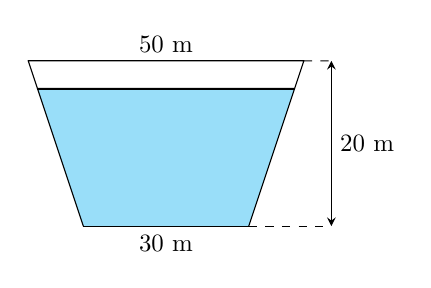
\begin{tikzpicture}[>=stealth,scale=0.7]
			 \def\BaseBot{3}
			 \def\BaseTop{5}
			\def\Height{3} 
			 \def\WaterLevel{2.5}
			\pgfmathsetmacro{\OffsetX}{0.5 *  (\BaseTop - \BaseBot)}
			 \pgfmathsetmacro{\Ratio}{(1 - \WaterLevel/\Height)}
			 \coordinate (A) at (-\BaseTop/2,\Height);
			\coordinate (B) at  (\BaseTop/2,\Height);
			\coordinate  (C) at (\BaseBot/2,0);
			 \coordinate (D) at (-\BaseBot/2,0);
			\pgfmathsetmacro{\XWL}{-\BaseTop/2 + \OffsetX * \Ratio} 
			\coordinate (WL1) at (\XWL,\WaterLevel); 
			\coordinate (WL2) at  (-\XWL,\WaterLevel);
			\fill[cyan!40] (D) --  (C) -- (WL2) -- (WL1) -- cycle;
			\draw  (D) -- (C);
			\draw[line width=1pt]  (WL1) -- (WL2);
			 \draw (D) -- (WL1);
			\draw (C)  -- (WL2);
			\draw[fill=white,draw] (WL1) -- (A) -- (B)  -- (WL2) -- cycle;
			\draw (A)  -- (B) node[midway,above] {$50$ m};
			\draw (D) --  (C) node[midway,below] {$30$ m};
			 \pgfmathsetmacro{\OffsetKichThuoc}{\BaseTop/2 + 0.5}
			 \coordinate (H1) at (\OffsetKichThuoc,0);
			\coordinate (H2) at  (\OffsetKichThuoc,\Height);
			\draw[<->] (H1) --  (H2) node[midway,right] {$20$ m};
			 \draw[dashed,thin] (B) -- (\OffsetKichThuoc,\Height);
			\draw[dashed,thin] (C)  -- (\OffsetKichThuoc,0);
		\end{tikzpicture}
	} 
	\shortans{4,4} 
	 \loigiai{
		Ta kẻ $A B$ song song với đáy và  kí hiệu các điểm như hình.
		\begin{center}
			\begin{tikzpicture}[>=stealth,line cap=round,line join=round]
					\def\BaseBot{3} 
					\def\BaseTop{5} 
					\def\Height{3} 
					 \def\WaterLevelHeight{2.5}
					\def\XPosHeight{0.8} 
					\pgfmathsetmacro{\SlopeOffset}{0.5 * (\BaseTop - \BaseBot) / \Height} 
					\def\BoxSize{0.1} 
					\coordinate (E) at (-\BaseBot/2,0); 
					\coordinate (F)  at (\BaseBot/2,0);
					\coordinate (M) at (-\BaseTop/2,\Height); 
					\coordinate (Q) at  (\BaseTop/2,\Height);
					\pgfmathsetmacro{\XWaterLeft}{-\BaseBot/2  - \SlopeOffset * \WaterLevelHeight}
					 \pgfmathsetmacro{\XWaterRight}{\BaseBot/2 + \SlopeOffset * \WaterLevelHeight}
					\coordinate  (WaterLeft) at (\XWaterLeft,\WaterLevelHeight);
					 \coordinate (WaterRight) at (\XWaterRight,\WaterLevelHeight);
					\pgfmathsetmacro{\XALeft}{-\BaseBot/2 - \SlopeOffset *  \XPosHeight}
					 \pgfmathsetmacro{\XARight}{\BaseBot/2 + \SlopeOffset * \XPosHeight}
					\coordinate  (A) at (\XALeft,\XPosHeight);
					\coordinate  (B) at (\XARight,\XPosHeight);
					\pgfmathsetmacro{\XN}{-\BaseTop/2 +  1}
					 \pgfmathsetmacro{\XP}{\BaseTop/2 - 1}
					\coordinate (N)  at (\XN,\Height);
					\coordinate (P) at  (\XP,\Height);
					 \coordinate (K) at (N |- A);
					\coordinate (FootP_Water) at (P |- WaterRight); 
					 \coordinate (FootP_A) at (P |- A);
					\fill[cyan!40] (E) -- (F) -- (Q) -- (M) --  cycle;
					\fill[white] (M) --  (Q) -- (WaterRight) -- (WaterLeft) -- cycle;
					\draw (E) -- (F)  -- (Q) -- (M) -- (E);
					\draw[line  width=1.5pt] (WaterLeft) -- (WaterRight);
					\draw[line width=0.8pt] (A)  -- (B);
					 \draw (N) -- (E);
					\draw (P) --  (FootP_Water);
					\draw (M) -- (Q) node[midway,above] {$50$  m};
					\draw (E) -- (F)  node[midway,below] {$30$ m};
					 \draw[dashed] (Q) -- (Q |- E);
					\draw[dashed] (Q  |- E) -- (F |- E);
					\draw[<->]  (Q |- E) -- (Q) node[midway,right] {$20$ m};
					\draw[dashed] (F)  -- (F |- E);
					\draw[<->] (B) -- (B |- F) node[midway,right] {$x$}; 
					\draw (P)--(F); 
					\coordinate (u)  at ($(FootP_Water)-(0.3,0)$);
					\coordinate (v)  at ($(FootP_A)-(0.3,0)$);
					\draw[<->] (u)  -- (v) node[midway,left] {$k (x)$};
					\node[above]  at (M) {$M$};
					\node[above] at  (Q) {$Q$};
					 \node[below] at (E) {$E$};
					\node[below] at (F) {$F$}; 
					\node[left] at (A) {$A$}; 
					\node[right] at (B)  {$B$};
					\node[above] at (N)  {$N$};
					\node[above] at (P)  {$P$};
					 \node[above right] at (K) {$K$};
					\draw (K) -- ($(K) +  (-\BoxSize,0)$) -- ($(K) + (-\BoxSize,\BoxSize)$) -- ($(K) + (0,\BoxSize)$) -- (K);
					\draw (N) -- ($(N) + (-\BoxSize,0)$) -- ($(N) + (-\BoxSize,-\BoxSize)$) -- ($(N) + (0,-\BoxSize)$) -- (N); 
					\draw (FootP_Water) -- ($(FootP_Water) + (\BoxSize,0)$) -- ($(FootP_Water)  + (\BoxSize,\BoxSize)$) -- ($(FootP_Water) + (0,\BoxSize)$) -- (FootP_Water);
					\draw (P) -- ($(P) +  (\BoxSize,0)$) -- ($(P) + (\BoxSize,-\BoxSize)$) -- ($(P) + (0,-\BoxSize)$) -- (P);
				\end{tikzpicture}
		\end{center}
		Vì nước cách đỉnh đập $4$ m nên độ  cao của nước trong hồ $h_0=20-4=16$ (m).\\
		Khi đó, $k(x)=16-x$,  $h(x)=AB$.\\
		Vì mặt cắt của đập có dạng hình thang cân, nên  khi kẻ $\heva{&EN\perp MQ\\&FP\perp MQ}$ thì $ENPF$ là hình chữ nhật và $\triangle EMN=\triangle FPQ$.\\
		Suy ra  $MN=\dfrac{MQ-NP}{2}=\dfrac{50-30}{2}=10$ (m).\\
		Suy ra $h(x)=AB=30+2AK$.\\ 
		Trong tam giác $EMN$, ta có $AK\parallel MN$ nên áp  dụng định lý Thales, ta có \[\dfrac{EK}{EN}=\dfrac{AK}{MN}\Rightarrow AK=\dfrac{EK\cdot MN}{EN}=\dfrac{10x}{20}=\dfrac{1}{2} x.\]
		Suy ra  $h(x)=30+x$.\\
		Khi đó áp suất tĩnh thủy  tác dụng lên đập nước là
		\[F=9\,800\displaystyle\int_0^{16}(16-x)(30+x)\mathrm{\, d}x=44\,322\,133{,}33\approx 4{,}4\cdot 10^7\text{ (N)}.\] 
		 Vậy $a=4{,}4$.
	 }
\end{bt}

% nguồn: Phan2_Lop_12_Dai_so_Chuong_4
\begin{bt}%[2D4V2-6]%[ma:8bfe8d2f]
	 \immini
	 {
	Mặt cắt ngang của một ống dẫn khí nóng là hình vành khuyên như hình vẽ. Khí bên trong ống được duy trì ở $150^{\circ} C$. Biết rằng nhiệt độ $T\left(^{\circ} C\right)$ tại điểm $A$ trên thành ống là hàm số của khoảng cách $x~(\mathrm{cm})$ từ $A$  đến tâm của mặt cắt và
	$$ 
	T^{\prime}(x)=-\dfrac{30}{x} \quad(6 \leq  x \leq 8).
	 $$
	(Nguồn: Y.A.Çengel, A.I.Gahjar,  Heat and Mass Transfer, Mc Graw Hill, 2015).
	} 
	{ 
	\begin{tikzpicture}[scale=.75,font=\footnotesize,line join=round,line cap=round,>=stealth,line width=1pt]
			 \coordinate (O) at (0,0);
			\draw[fill=yellow,name path=C1]  (O) circle (3 cm);
			\draw[name  path=C2] (O) circle (2 cm);
			\draw[name path=C3,dashed]  (O) circle (2.7 cm);
			\draw[fill=white,name  path=C1] (O) circle (2.4 cm);
			\coordinate (A)  at ($(O) + (40:2.7)$);
			 \coordinate (B) at ($(O) + (110:2.4)$);
			\coordinate (C)  at ($(O) + (190:3)$);
			 \draw (O)--(A) node[sloped,pos=.5,below,font=\small] {$x$ cm};
			\draw  (O)--(B) node[sloped,pos=.5,above,font=\small] {$6$ cm};
			\draw (O)--(C) node[sloped,pos=.4,below,font=\small]  {$8$ cm};
			\draw  (43:2.9) node[right,font=\small] {$A$};
		\end{tikzpicture}
	} 
	 \noindent
	Tìm nhiệt độ mặt ngoài của ống (làm tròn đến hàng đơn  vị). \shortans{141}
	 \loigiai{
		Ta  có $T(6)=150$ (khí bên trong ống được duy trì ở $150^{\circ} C$).
		$$ 
		\begin{aligned}
			T(8)-T(6) &=\displaystyle\int_6^{8} T^{\prime}(x) \mathrm{\,d}x=\displaystyle\int_6^{8}\left(-\dfrac{30}{x}\right) \mathrm{\,d} x  \\
			&=-30 \displaystyle\int_6^{8}\dfrac{1}{x} \mathrm{\,d}  x \\
			&=\left.-30\ln x\right|_6 ^{8}\approx  -8{,}63.
		\end{aligned}
		$$ 
		Suy  ra $ T(8)=T(6)-8{,}63\approx 141$ ($^{\circ} C$).\\
		Vậy nhiệt độ  mặt ngoài của ống là $141^{\circ} C$.
	 }
\end{bt}

% nguồn: Phan2_Lop_12_Dai_so_Chuong_4
\begin{bt}%[2D4V2-6]%[ma:88cc41ac]
	Cây cà chua khi trồng có chiều cao $5$ cm . Tốc độ tăng chiều cao của cây cà chua sau khi trồng được cho bởi  hàm số $v(t)=-0,1 t^3+t^2$, trong đó $t$ tính theo tuần, $v(t)$ tính bằng centimét/tuần. Gọi $h(t)$ là độ cao của cây cà chua ở tuần thứ $t$. Vào thời điểm cây cà chua đó phát triển nhanh nhất thì cây cà chua cao bao nhiêu centimét? (làm tròn kết quả đến hàng phần mười).
	\shortans{88,3} 
	 \loigiai{
		Ta có $h(t)=\displaystyle\int \left(-0,1 t^3+t^2\right)\mathrm{\,d}t =\dfrac{-t^4}{40}+\dfrac{t^3}{3}+C$.\\ 
		Cây cà chua khi trồng  có chiều cao $5$ cm nên $h(0)=5 \Rightarrow C=5$.\\
		Do đó  $h(t)=\dfrac{-t^4}{40}+\dfrac{t^3}{3}+5$.\\
		Ta cần tìm giá trị lớn nhất của $h(t)=\dfrac{-t^4}{40}+\dfrac{t^3}{3}+5$ với $t \in[0; 10]$.\\ 
		Ta có $h'(t)=\dfrac{-t^3}{10}+t^2$ $\Rightarrow h'(t)=0 \Leftrightarrow \hoac{&t=0\\&t=10.}$\\ 
		Ta thấy  $h(0)=5$, $h(10)=\dfrac{265}{3}$.\\
		Khi đó, $h(t)$ đạt  giá trị lớn nhất bằng $\dfrac{265}{3}$ trên đoạn $[0; 10]$.\\
		Vậy chiều cao tối đa của cây cà chua đó là $\dfrac{265}{3} \approx  88,3 (\text{cm})$.
	} 
\end{bt}

% nguồn: Phan2_Lop_12_Dai_so_Chuong_4
\begin{bt}%[2D4V2-6]%[ma:205df431]
	Một lực $30$ (N) cần thiết để kéo giãn một lò xo thêm $4$ (cm) so với chiều dài tự nhiên  $18$ cm. Hãy tìm công cần thiết là bao nhiêu Jun (J) để kéo giãn lò xo từ chiều dài $20$ cm đến $24$ cm.
	\begin{center}
		\begin{tikzpicture}[line join=round,line cap=round,>=stealth,font=\footnotesize,scale=1.2,spring/.style={decorate,decoration={snake,amplitude=2mm,segment length=3mm,pre length=1mm,post length=1mm}}]
				\fill[pattern=north east lines,pattern  color=gray] (-0.3,-0.4) rectangle (0,0.4);
				\draw (0,-0.4) -- (0,0.4); 
				\draw (2,-0.1)  -- (2,0.1);
				\draw  (2,-2.1) -- (2,-1.9);
				\draw (3.5,-2.1)  -- (3.5,-1.9);
				\draw[->] (-0.2,0) --  (4.5,0) node[below left] {$x$};
				 \draw[spring] (0,0) -- (2,0);
				\node[below=2pt  of {(2,0)}] {$0$};
				\node[below=0.6cm of {(-1,0)},anchor=north west] {(a) Lò xo chưa bị kéo giãn (trạng thái  tự nhiên)};
				\fill[pattern=north east lines,pattern color=gray] (-0.3,-2.4) rectangle (0,-1.6); 
				 \draw[spring] (0,-2) -- (3.5,-2);
				\node[below=2pt of {(2,-2)}] {$0$}; 
				 \draw (2,-2) -- (2,-2);
				\draw (0,-2.4) --  (0,-1.6);
				\draw[->] (-0.2,-2) --  (4.5,-2) node[below left] {$x$};
				\draw  [|<->|] (2,-1.6) -- (3.5,-1.6) node[midway,above]{$x$};
				\node[below=0.6cm of {(-1,-2)},anchor=north west] {(b) Lò xo được kéo  giãn thêm $x$ đơn vị so với chiều dài tự nhiên.};
			\end{tikzpicture}
	\end{center}
	\shortans{1,2} 
	\loigiai{ 
		Giả sử đặt lò  xo trùng với trục $Ox$ và đầu tự do ở gốc toạ độ (như Hình b).\\
		Theo định luật Hooke, lực $F(x)$ cần để kéo giãn lò xo thêm  $x$ mét so với chiều dài tự nhiên là $F(x)=kx$.\\
		Vì cần lực  $30$ N để kéo giãn lò xo $4$ cm, tức $0{,}04$ m.\\
		Nên ta có $30=k\cdot 0{,}04  \Rightarrow k=750$ (N/m).\\
		Do  đó $F(x)=750x$.\\
		Công để  kéo giãn từ $20$ cm đến $24$ cm (tức $x$ tăng từ $0{,}02$ m đến $0{,}06$ m) là
		 $$W=\displaystyle\int_{0{,}02}^{0{,}06} F(x)\mathrm{\,d}x=\displaystyle\int_{0{,}02}^{0{,}06} 750x\mathrm{\,d}x=750\dfrac{1}{2}x^2 \bigg|_{0{,}02}^{0{,}06}=375\left[(0{,}06)^2-(0{,}02)^2\right] =1,2 \,\, \text{ (J)}.$$
		Vậy công  cần thiết là $1{,}2$ (J).
	} 
\end{bt}

% nguồn: Phan2_Lop_12_Dai_so_Chuong_4
\begin{bt}%[2D4V2-6]%[ma:a8af324a]
	\immini[thm]{Nhà Tí có một bồn chứa nước hình trụ cao $300$ cm, đường kính $60$ cm. Bồn đầy nước thì bạn Tí vô ý mở van xả. Mực nước hạ với vận tốc $h'(t)=\dfrac{1}{54} t-\dfrac{10}{3}$ ($t$ tính bằng phút, $h'(t)$ cm/ phút). Sau $1{,}5$ giờ (tức $90$ phút) thì Tí mới phát hiện sự cố.  Hỏi lượng nước đã mất là bao nhiêu lít \textit{(làm tròn kết quả đến hàng đơn vị)}?}{
	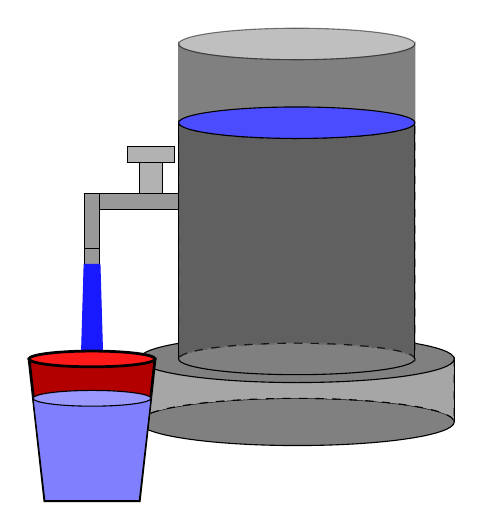
\begin{tikzpicture}[>=stealth,scale=1]
			 \pgfmathsetmacro{\BaseHeight}{0.8}
			 \pgfmathsetmacro{\BaseRadius}{2.0}
			 \pgfmathsetmacro{\TankHeight}{4.0}
			 \pgfmathsetmacro{\TankRadius}{1.5}
			\pgfmathsetmacro{\WaterLevel}{3.0} 
			 \pgfmathsetmacro{\GlassTopRadius}{0.8}
			\pgfmathsetmacro{\GlassBaseRadius}{0.6} 
			\pgfmathsetmacro{\GlassHeight}{1.8} 
			 \pgfmathsetmacro{\WaterInGlassHeight}{1.3}
			 \pgfmathsetmacro{\TankBaseY}{0}
			 \pgfmathsetmacro{\TankBaseZ}{\TankBaseY + \BaseHeight}
			\pgfmathsetmacro{\TankTopY}{\TankBaseZ + \TankHeight} 
			 \pgfmathsetmacro{\TapAttachX}{-\TankRadius}
			\pgfmathsetmacro{\TapY}{\TankBaseZ  + \TankHeight/2}
			\pgfmathsetmacro{\TapOutX}{\TapAttachX - 1.0} 
			\pgfmathsetmacro{\TapOutY}{\TapY  - 0.7}
			\pgfmathsetmacro{\GlassBaseY}{-1.0} 
			\pgfmathsetmacro{\GlassX}{\TapOutX -  0.1}
			\pgfmathsetmacro{\WaterInGlassSurfaceY}{\GlassBaseY +  \WaterInGlassHeight}
			\pgfmathsetmacro{\WaterTop}{\TankBaseZ  + \WaterLevel}
			\pgfmathsetmacro{\WaterInGlassRadius}{0.75} 
			\pgfmathsetmacro{\GlassTopY}{\GlassBaseY +  \GlassHeight}
			\draw[fill=gray]  (0,\TankBaseY) ellipse (\BaseRadius cm and 0.3cm);
			 \draw[fill=gray!70,dashed]
				(-\BaseRadius,\TankBaseY) -- (-\BaseRadius,\TankBaseZ) arc (180:360:\BaseRadius cm and 0.2cm)  -- (\BaseRadius,\TankBaseY) arc (0:180:\BaseRadius cm and 0.3cm);
			\draw  (\BaseRadius,\TankBaseY) -- (\BaseRadius,\TankBaseZ);
			\draw[fill=gray] (0,\TankBaseZ) ellipse (\BaseRadius  cm and 0.3cm);
			\draw (0,\TankBaseZ) ellipse  (\TankRadius cm and 0.2cm);
			\draw[fill=green!10!white,draw,gray] (-\TankRadius,\TankBaseZ) -- (-\TankRadius,\TankTopY) arc (180:360:\TankRadius cm and  0.2cm) -- (\TankRadius,\TankBaseZ) arc (0:180:\TankRadius cm and 0.2cm);
			 \draw[fill=gray,opacity=0.5] (0,\TankTopY) ellipse (\TankRadius cm and 0.2cm);
			\draw[fill=gray!70!black,opacity=0.8,dashed] 
				(-\TankRadius,\TankBaseZ) -- (-\TankRadius,\WaterTop)  arc (180:360:\TankRadius cm and 0.2cm) -- (\TankRadius,\TankBaseZ) arc (0:180:\TankRadius cm and 0.2cm);
			\draw[fill=blue!70!white] (0,\WaterTop) ellipse (\TankRadius cm and  0.2cm);
			\draw (-\TankRadius,\TankBaseZ)  -- (-\TankRadius,\WaterTop)
				(\TankRadius,\TankBaseZ) --  (\TankRadius,\WaterTop);
			\draw[fill=gray!80,draw] (\TapAttachX,\TapY - 0.1) rectangle (\TapOutX,\TapY + 0.1); 
			\draw[fill=gray!80] (\TapOutX,\TapY + 0.1) -- (\TapOutX,\TapOutY + 0.1) -- (\TapOutX - 0.2,\TapOutY + 0.1) -- (\TapOutX -  0.2,\TapY + 0.1) -- cycle;
			\draw[fill=gray!80,draw] (\TapOutX,\TapOutY + 0.1) -- (\TapOutX,\TapOutY  - 0.1) -- (\TapOutX - 0.2,\TapOutY - 0.1) -- (\TapOutX - 0.2,\TapOutY + 0.1) -- cycle;
			\draw[fill=gray!60,draw] (\TapAttachX -  0.5,\TapY + 0.1) rectangle (\TapAttachX - 0.2,\TapY + 0.5);
			\draw[fill=gray!60,draw] (\TapAttachX  - 0.65,\TapY + 0.5) rectangle (\TapAttachX - 0.05,\TapY + 0.7);
			\pgfmathsetmacro{\StreamWidthStart}{0.2} 
			\pgfmathsetmacro{\StreamWidthEnd}{0.3} 
			 \draw[fill=blue!50,draw,blue!90]
				 (\TapOutX - \StreamWidthStart/2 - 0.1,\TapOutY - 0.1) --
				(\TapOutX + \StreamWidthStart/2 - 0.1,\TapOutY -  0.1) --
				(\GlassX + \StreamWidthEnd/2,\WaterInGlassSurfaceY)  --
				(\GlassX - \StreamWidthEnd/2,\WaterInGlassSurfaceY)  -- cycle;
			 \draw[line width=1pt,fill=red!70!black,draw]
				(\GlassX  - \GlassTopRadius,\GlassTopY) --
				(\GlassX +  \GlassTopRadius,\GlassTopY) --
				(\GlassX + \GlassBaseRadius,\GlassBaseY)  --
				(\GlassX - \GlassBaseRadius,\GlassBaseY) --  cycle;
			\draw[line  width=1pt,fill=red!90!white,draw] (\GlassX,\GlassTopY) ellipse (\GlassTopRadius cm and 0.1cm);
			 \draw[fill=blue!50!white]
				(\GlassX -  \WaterInGlassRadius,\WaterInGlassSurfaceY) --
				(\GlassX + \WaterInGlassRadius,\WaterInGlassSurfaceY)  --
				(\GlassX  + \GlassBaseRadius,\GlassBaseY) --
				(\GlassX - \GlassBaseRadius,\GlassBaseY)  -- cycle;
			\draw[fill=blue!40] (\GlassX,\WaterInGlassSurfaceY) ellipse (\WaterInGlassRadius cm and  0.1cm);
		\end{tikzpicture}
	} 
	 \shortans{636}
	\loigiai{ 
		Ta có bán kính của bồn  chứa nước hình trụ là $r=\dfrac{60}{2}=30$ cm.\\
		Ta có  $h(t)=\displaystyle\int\left(\dfrac{1}{54} t-\dfrac{10}{3}\right) \mathrm{\,d}t=\dfrac{1}{108} t^2-\dfrac{10}{3} t+C$.\\
		Do bồn ban đầu đầy  $h(0)=300 \Rightarrow C=300$.\\
		Vậy $h(t)=\dfrac{1}{108} t^2-\dfrac{10}{3} t+300$.\\ 
		Lượng  nước mất sau $1{,}5$ giờ là
		độ giảm mực nước \[\Delta  h=\displaystyle\int_0^{90} h'(t) \mathrm{\,d} t=h(t)\bigg|_0 ^{90}=h(90)-(0)=75-300=-225\text{ (cm)}.\]
		Thể tích nước mất  $
		 \Delta V=\pi r^2 \Delta h=\pi \cdot 30^2 \cdot 225=202\,500 \pi \text{ cm}^3 \approx 636$ lít.
	} 
\end{bt}

% nguồn: Phan2_Lop_12_Dai_so_Chuong_4
\begin{bt}%[2D4V2-6]%[ma:1c7cb1c8]
	Ta biết rằng hàm cầu liên quan đến giá $p$ của một sản phẩm với nhu cầu của người tiêu dùng, hàm cung liên quan đến giá $p$ của sản phẩm với mức độ sẵn sàng cung cấp sản phẩm của nhà sản xuất. Điểm cắt  nhau $(x_0;p_0)$ của đồ thị hàm cầu $p=D(x)$ và đồ thị hàm cung $p=S(x)$ được gọi là điểm cân bằng. Các nhà kinh tế học gọi diện tích của hình giới hạn bởi đồ thị hàm cầu, đường ngang $p=p_0$ và đường thẳng $x=0$ là thặng dư tiêu dùng.
	\begin{center}
		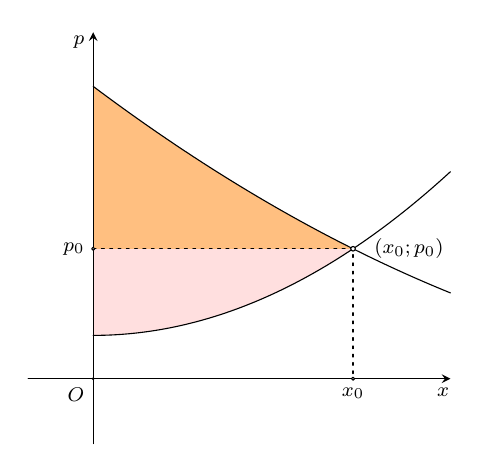
\begin{tikzpicture}[scale=0.55,x=1.5cm,>=stealth,line join=round,line cap=round,font=\footnotesize]
				 \def\xmin{-1}
				\def\xmax{5.5} 
				 \def\ymin{-1.5}
				 \def\ymax{8}
				 \def\f{.125*(\x)^2+1}
				 \def\g{3/64*(\x)^2-9/8*(\x)+27/4}
				\fill [pink!50]  (0,1) plot [domain=0:4] (\x,{\f})--(0,3)--cycle;
				\fill  [orange!50] (0,27/4) plot [domain=0:4] (\x,{\g})--(0,3)--cycle;
				 \draw [->] (\xmin,0)--(\xmax,0) node [below,xshift=-3pt] {$x$};
				\draw [->] (0,\ymin)--(0,\ymax) node  [left,yshift=-4pt] {$p$};
				\fill (0,0)  circle (1pt) node [below left] {$O$};
				\draw [smooth,samples=100]  plot [domain=0:\xmax] (\x,{\f}) plot [domain=0:\xmax] (\x,{\g});
				\draw [dash pattern=on 1pt off 2pt] (0,3) node [left] {$p_0$}--(4,3) node [right=5pt] {$(x_0;  p_0)$}--(4,0) node [below] {$x_0$};
				\draw [fill=white] (0,3) circle (1pt) 
					(4,0) circle (1pt) 
					(4,3)  circle (1.5pt);
			\end{tikzpicture}
	\end{center}
	Giả sử hàm cung và hàm cầu của một loại  sản phẩm được mô hình hóa bởi:
	Hàm cầu $p=-0{,}36x+9$ và hàm cung $p=0{,}14x+2$, trong đó $x$ là đơn vị sản phẩm. Tìm thặng dư tiêu dùng cho loại sản  phẩm này (làm tròn đến hàng phần mười).
	 \shortans{35,3}
	\loigiai{ 
		Để  tìm thặng dư tiêu dùng, trước hết ta cần xác định điểm cân bằng của thị trường.\\
		Điểm cân bằng là điểm mà tại  đó hàm cung bằng hàm cầu:
		\allowdisplaybreaks 
		\begin{eqnarray*}
			&&-0{,}36x+9=0{,}14x+2 \\ 
			&\Leftrightarrow&  7=0{,}5x \\
			&\Leftrightarrow& x_0=\dfrac{7}{0{,}5}=14. 
		\end{eqnarray*}
		Vậy,  điểm cân bằng là $(14; 3{,}96)$.\\
		Thặng dư tiêu dùng là 
		 \allowdisplaybreaks
		\begin{eqnarray*}
			S&=&\displaystyle\int_0^{x_0}  \left[D(x)-p_0\right] \mathrm{\,d}x=\displaystyle\int_0^{14} [(-0{,}36x+9)-3{,}96] \mathrm{\,d}x \approx35{,}3.
		\end{eqnarray*}
	 }
\end{bt}

% nguồn: Phan2_Lop_12_Dai_so_Chuong_4
\begin{bt}%[2D4V2-6]%[ma:94173241]
	\immini{Cho ba Parabol $\left(P_1\right) \colon y = x^2$; $\left(P_2\right)\colon y = 2x^2$; $\left(P_3\right) \colon y = kx^2$ với $k > 2$. Gọi $P$ là điểm bất kỳ thuộc parabol $\left(P_2\right)$ và $S_1$, $S_2$ là diện tích các miền phẳng $\left(H_1\right)$, $\left(H_2\right)$ (các miền được gạch chéo trong hình vẽ). Nếu $S_1 = S_2$ thì giá trị của $k = \dfrac{a}{b}$ với $a$, $b \in \mathbb{N}$ và $\dfrac{a}{b}$ là phân số tối giản. Tính $a + b$. 
	 }
	{\begin{tikzpicture}[>=stealth,line join=round,line cap=round,color=blue,font=\footnotesize,scale=1.2]
		\draw[->] (-0.5,0) --  (3,0) node[below] {$x$};
		\draw[->] (0,-0.5)--(0,4) node[right]{$y$}; 
		\draw (0,0) node[below  left]{$O$};
		\draw (1,2) node[above  right]{$P$};
		\fill[pattern = north east lines,pattern color=cyan,smooth] (0,0)  --plot[domain=0:1] (\x,{2*(\x)^2})-- (0.75,2)--plot[domain=0.75:0] (\x,{3.5*(\x)^2})--cycle;
		\fill[pattern =  north west lines,pattern color=red,smooth] (0,0) --plot[domain=0:1] (\x,{(\x)^2})--(1,2)--plot[domain=1:0] (\x,{2*(\x)^2})--cycle;
		\draw[violet,samples=150,smooth,domain=-0:1.9] plot  (\x,{(\x)^2});
		 \draw[violet,samples=150,smooth,domain=-0:1.35] plot (\x,{2*(\x)^2});
		 \draw[violet,samples=150,smooth,domain=-0:1.02] plot (\x,{3.5*(\x)^2});
		 \draw[dashed] (1,0)--(1,2)--(0,2);
		\draw[->] (0.8,0.9)--(1.3,0.6) node[below right]{\scriptsize  $(H_1)$};
		 \draw[->] (0.7,1.3)--(0.3,1.4) node[above]{\scriptsize $(H_2)$};
		\draw (0.9,3.6) node[above]{\scriptsize $(P_3)$}; 
		 \draw (1.45,3.6) node[above]{\scriptsize $(P_2)$};
		\draw  (2.0,3.6) node[above]{\scriptsize $(P_1)$};
	\end{tikzpicture}
	 }
	\shortans{41} 
	\loigiai{ 
		 Gọi $P\left(x_o; y_o\right) \Rightarrow y_o = 2 x_o^2$.\\
		Hình phẳng $(H_1)$ giới hạn bởi $x = 0$; $x = x_o$; $\left(P_1\right) \colon y = x^2$; $\left(P_2\right) \colon y =  2 x^2$.\\
		Suy ra  diện tích hình phẳng $\left(H_1\right)$ là $S_{\left(H_1\right)} = \displaystyle\int_0^{x_o} \left(2x^2 - x^2\right) \mathrm{\,d}x
		 = \dfrac{x_o^2}{3}$.\\
		Hình phẳng $(H_2)$ giới hạn bởi $y = 0$; $y = 2x_o^2$; $\left(P_2\right) \colon y = 2x^2$; $\left(P_3\right) \colon  y = k x^2$.\\
		Suy  ra diện tích hình phẳng $\left(H_2\right)$ là $$S_{\left(H_2\right)} = \displaystyle\int_0^{2x_o^2} \left(\sqrt{\dfrac{y}{2}} - \sqrt{\dfrac{y}{k}}\right) \mathrm{\,d}y
		=  \left(\dfrac{\sqrt{2}}{3}y\sqrt{y} - \dfrac{2}{3\sqrt{k}}y \sqrt{y}\right) \Big|_0 ^{2x_o^2} = \left(\dfrac{\sqrt{2}}{3} - \dfrac{2}{3\sqrt{k}}\right) 2\sqrt{2}x_0^3.$$
		Theo giải  thiết $S_1 = S_2$ nên ta có
		$$\left(\frac{\sqrt{2}}{3}-\frac{2}{3 \sqrt{k}}\right) 2 \sqrt{2} x_o^3 = \frac{x_o^3}{3} \Leftrightarrow 4 - \dfrac{4 \sqrt{2}}{\sqrt{k}} = 1 \Leftrightarrow \sqrt{k} =  \dfrac{4\sqrt{2}}{3} \Leftrightarrow k= \dfrac{32}{9}.$$
		Khi đó $\heva{&a = 32\\&b = 9} \Rightarrow a + b =  41$.
	} 
\end{bt}

% nguồn: Phan2_Lop_12_Dai_so_Chuong_4
\begin{bt}%[2D4V2-6]%[ma:d917c1ff]
	Một xe ô tô sau khi chờ hết đèn đỏ đã bắt đầu chuyển động  với vận tốc được biểu thị bằng đồ thị là đường cong parabol như hình bên dưới. Biết rằng sau $5$ phút thì xe đạt đến vận tốc cao nhất
	$1\,000$ m/phút và bắt đầu giảm vận tốc, đi được $6$ phút thì xe chuyển  động đều. Hỏi quãng đường xe đã đi được trong khoảng $10$ phút đầu tiên là bao nhiêu mét?
	\begin{center}
		\begin{tikzpicture}[scale=0.5,font=\footnotesize,line join=round,line cap=round,>=stealth]
				\path 
					(0,0)  coordinate (O) node[below left]{$O$}
					(5,10) coordinate (A) 
					 (6,9.6) coordinate (B)
					(10,9.6) coordinate (C); 
				 \draw[->] (0,-1)--(0,11) node[right]{$v$};
				 \draw[->] (-1,0)--(11,0) node[below]{$t$};
				\draw[blue,smooth,samples=100,domain=0:6] plot  (\x,{-0.4*(\x)^2+4*(\x)});
				 \draw[blue] (B)--(C);
				\draw[dashed]  (0,10) node[left]{$1\,000$}--(A)--(5,0) node[below]{$5$}
					(B)--(6,0)  node[below]{$6$}
					(C)--(10,0) node[below]{$10$}; 
				\foreach \p in {A,B,C,O} 
				\fill  (\p) circle (1.2pt);
			\end{tikzpicture}
	\end{center}
	 \shortans{8160}
	 \loigiai{
		Gọi phương trình vận tốc của ô tô là $v(t)=at^2+bt+c$, với $a$,  $b$, $c$ là các số thực, $a<0$ và $t \in [0;6]$.\\
		Theo đề ta  có hệ phương trình
		$$\heva{&v(0)=0\\&v(5)=1\,000\\&-\dfrac{b}{2a}=5}\Leftrightarrow  \heva{&c=0\\&25a+5b+c=1\,000\\&10a+b=0}\Leftrightarrow \heva{&a=-40\\&b=400\\&c=0.}$$
		Suy  ra phương trình vận tốc của ô tô là $v(t)=-40t^2+400t$ với $t \in [0;6]$.\\
		Suy ra $v(6) =  960$. \\
		Trong khoảng $6$ phút  đầu phương trình quãng đường là $${S(t) = \displaystyle\displaystyle\int\left(-40t^2 + 400t\right)\mathrm{\,d}t = -\dfrac{40}{3}t^3 + 200t^2 + C}.$$
		Tại thời điểm xe ô tô xuất phát, ta có $S(0) = 0$ suy  ra $C = 0$ nên phương trình quãng đường là ${S(t) = -\dfrac{40}{3}t^3 + 200t^2}$ (m).\\
		Trong khoảng $6$ phút đầu ô tô đi được quãng đường là $S(6) =  4\,320$ m và $4$ phút tiếp theo ô tô đi được quãng đường là $960\cdot 4 = 3\,840$ m.\\
		Vậy quãng đường ô tô đi được trong $10$ phút đầu là ${4\,320 + 3\,840 = 8\,160}$ m. 
	 }
\end{bt}

% nguồn: Phan2_Lop_12_Dai_so_Chuong_4
\begin{bt}%[2D4V2-6]%[ma:6763ee42]
	Tại một nhà máy, gọi $C(x)$ là tổng chi phí (tính theo triệu đồng) để  sản xuất $x$ tấn sản phẩm $A$ trong một tháng. Khi đó, đạo hàm $C'(x)$, gọi là chi phí cận biên, cho biết tốc độ gia tăng tổng chi phí theo lượng gia tăng sản phẩm được sản xuất. Giả sử chi phí cận biên (tính theo triệu đồng trên tấn) của nhà máy được ước lượng bởi công thức
	$C'(x)=5-0{,}06 x+0{,}00072 x^2$, $0 \le  x \le 150$.
	Biết rằng $C(0)=30$ triệu đồng, gọi là chi phí cố định. Tính tổng chi phí khi nhà máy sản xuất $100$ tấn sản phẩm A trong  tháng.
	\shortans{470} 
	\loigiai{ 
		 Ta có
		\begin{eqnarray*}
			C(100)-C(0)&=&\displaystyle\int_0^{100}  C'(x)\mathrm{\, d}x\\
			&=&\displaystyle\int_0^{100}\left(5-0,06 x+0,00072  x^2\right)\mathrm{\, d}x\\
			 &=&5 \displaystyle\int_0^{100}\mathrm{\, d}x-0,06 \displaystyle\int_0^{100} x\mathrm{\, d}x+0,00072 \displaystyle\int_0^{100} x^2\mathrm{\, d}x\\
			&=&5  x\bigg|_0^{100}-0{,}03 x^2\bigg|_0^{100}+0{,}00024 x^3\bigg|_0^{100}=440.
		\end{eqnarray*}
		Suy  ra $C(100)=C(0)+440=30+440=470$ (triệu đồng).\\
		Vậy khi nhà  máy sản xuất $100$ tấn sản phẩm A trong tháng thì tổng chi phí là $470$ triệu đồng.
	} 
\end{bt}

% nguồn: Phan2_Lop_12_Dai_so_Chuong_4
\begin{bt}%[2D4V2-6]%[ma:c50b0a79]
	Từ hình chữ nhật $ABCD$ có chiều dài $AB=8$ cm và chiều  rộng $BC=4$ cm, người ta cắt bỏ miền $(R)$ được giới hạn bởi cạnh $CD$ của hình chữ nhật và hai nửa đường parabol có chung đỉnh là trung điểm cạnh $AB$, chúng lần lượt đi qua hai đầu mút $C$, $D$ của hình chữ nhất đó (phần tô đậm như hình vẽ). Phần còn lại cho quay quanh trục $AB$ để tạo nên một đồ vật làm trang trí, thể tích của vật trang trí đó bằng bao nhiêu cm$^3$. Viết kết quả làm tròn đến hàng đơn vị.
	\begin{center}
		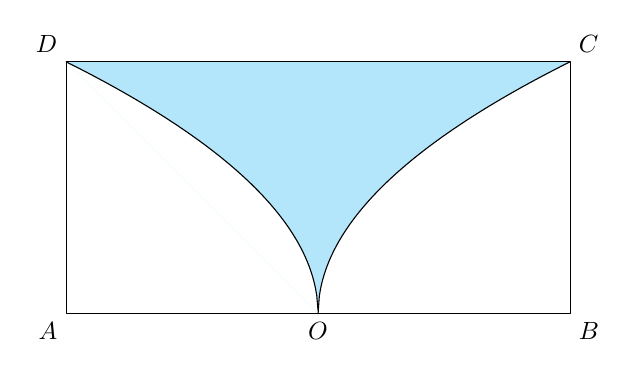
\begin{tikzpicture}[scale=0.8,line join=round,line cap=round,>=stealth]
				\coordinate  (A) at (-4,0);
				\coordinate  (B) at (4,0);
				\coordinate (C) at  (4,4);
				 \coordinate (D) at (-4,4);
				\coordinate  (O) at (0,0);
				 \fill[cyan!30]
					(O) 
					 plot[domain=0:4,samples=200] (\x,{sqrt (4*\x)})
					-- (C) --  (D)
					plot[domain=-4:0,samples=200] (\x,{sqrt  (-4*\x)})
					-- (O); 
				\draw  (A)--(B)--(C)--(D)--cycle;
				\draw plot[domain=0:4,samples=200] (\x,{sqrt  (4*\x)});
				\draw plot[domain=-4:0,samples=200] (\x,{sqrt (-4*\x)}); 
				\node[below left] at (A) {$A$}; 
				\node[below  right] at (B) {$B$};
				\node[above right] at (C)  {$C$};
				\node[above left] at (D)  {$D$};
				\node[below] at (O)  {$O$};
			\end{tikzpicture}
	\end{center}
	\shortans{201} 
	\loigiai{ 
		\begin{center}
			\begin{tikzpicture}[scale=0.8,line join=round,line cap=round,>=stealth]
					\coordinate (A) at  (-4,0);
					\coordinate (B) at  (4,0);
					\coordinate (C)  at (4,4);
					\coordinate (D)  at (-4,4);
					\coordinate (O) at  (0,0);
					\fill[cyan!30] 
						 (O)
						plot[domain=0:4,samples=200] (\x,{sqrt  (4*\x)})
						-- (C) --  (D)
						plot[domain=-4:0,samples=200]  (\x,{sqrt (-4*\x)})
						--  (O);
					\draw  (A)--(B)--(C)--(D)--cycle;
					 \draw[->] (O)--($(O)!1.3!(B)$) node[below]{$x$};
					\draw[->]  (-90:1)--(90:5) node[right]{$y$};
					\draw  plot[domain=0:4,samples=200] (\x,{sqrt (4*\x)});
					\draw plot[domain=-4:0,samples=200]  (\x,{sqrt (-4*\x)});
					\node[below  left] at (A) {$A$};
					\node[below right] at (B) {$B$}; 
					 \node[above right] at (C) {$C$};
					\node[above left] at (D)  {$D$};
					\node[below right] at  (O) {$O$};
				\end{tikzpicture}
		\end{center}
		Dựng hệ trục tọa độ $Oxy$ như hình vẽ. Phương trình  Parabol $OC$ có dạng $y^2=ax.$\\
		Mặt khác, Parabol đi qua  điểm $C(4;4) \Rightarrow 4^2=4a \Rightarrow a=4$\\
		Khi đó phương trình đường cong OC là  $y=\sqrt{4x}.$\\
	Thể tích của vật  thể thu được là \[V=2\left(\pi \displaystyle\int_0^4 (\sqrt{4x})^2 \mathrm{\,d}x\right)=64\pi \approx 201(\text{cm}^3).\]}
\end{bt}

% nguồn: Phan2_Lop_12_Dai_so_Chuong_4
\begin{bt}%[2D4V2-6]%[ma:c86f3b0f]
	Một vật chuyển động trong $4$ giờ với vận tốc $v$ (km/h) phụ thuộc vào thời gian $t(h)$ có đồ thị vận tốc là một đường parabol có đỉnh $I(3;10)$ và trục đối xứng vuông góc với trục hoành như hình vẽ. Tính quãng  đường vật di chuyển được trong nửa thời gian sau của chuyển động đó (kết quả làm tròn đến hàng phần chục và tính theo đơn vị km).
	\begin{center}
		\begin{tikzpicture}[scale=0.6,font=\footnotesize,line join=round,line cap=round,>=stealth]
				 \path
					 (0,0) coordinate (O) node[below left]{$O$}
					(3,10)  coordinate (A)
					(0,1) coordinate  (B) node[left]{$1$};
				\draw[->] (0,-1)--(0,11)  node[right]{$v$};
				\draw[->] (-1,0)--(5,0) node[below]{$t$}; 
				 \draw[blue,smooth,samples=100,domain=0:4] plot (\x,{-1*(\x)^2+6*(\x)+1});
				\draw[dashed] (0,10)  node[left]{$10$}--(A)--(3,0) node[below]{$3$};
				\foreach  \p in {A,B,O}
				\fill (\p) circle (1.2pt); 
			\end{tikzpicture}
	\end{center}
	 \shortans{19,3}
	\loigiai{ 
		Gọi phương trình vận tốc của vật là $v(t)=at^2+bt+c$, với $a$, $b$, $c$ là các số thực, $a<0$ và $t \in  [0;4]$.\\
		Theo đề ta có hệ  phương trình
		$$\heva{&v(0)=1\\&v(3)=10\\&-\dfrac{b}{2a}=3}\Leftrightarrow \heva{&c=1\\&9a+3b+c=10\\&6a+b=0}\Leftrightarrow  \heva{&a=-1\\&b=6\\&c=1.}$$
		Suy ra phương trình vận tốc của vật là $v(t)=-t^2+6t+1$, với $t  \in [0;4]$.\\
		Quãng đường $s(t)$ vật di chuyển được  trong thời gian $4$ giờ là một nguyên hàm của $v(t), t \in [0;4]$.\\
		Ta có  $s(t) = \displaystyle\int \left(-t^2+6t+1\right)\mathrm{\,d}t=-\dfrac{t^3}{3}+3t^2+t+C$.\\
		Quãng đường vật di chuyển được trong  $2$ giờ đầu là $s(2) = \dfrac{34}{3} + C$ (km).\\
		Quãng đường vật  di chuyển được trong $4$ giờ là $s(4) = \dfrac{92}{3} + C$ (km).\\
		 Vậy quãng đường vật di chuyển được trong nửa thời gian sau của chuyển động là
		$$s(4) - s(2)  = \dfrac{58}{3} \approx 19{,}3 \text{ (km)}.$$
	 }
\end{bt}

% nguồn: Phan2_Lop_12_Dai_so_Chuong_4
\begin{bt}%[2D4V2-6]%[ma:e8132967]
	Khi nghiên cứu dịch sốt xuất huyết ở một địa phương, các chuyên gia y tế ước tính rằng tại ngày thứ $m$ có $F(m)$ người mắc bệnh (sau khi đã làm tròn đến chữ số hàng đơn vị). Biết rằng tốc độ lan truyền bệnh là $F’(m)=\dfrac{150}{2 m+1}$ và ngày đầu tiên $(m=0)$ người ta phát hiện ra $50$ bệnh nhân. Hãy  xác định số người mắc bệnh ở ngày thứ $10$.
	\shortans{278} 
	 \loigiai{
		Từ giả thiết ta có $ F(m)= \displaystyle\int F'(m)\mathrm{\,d}m =\displaystyle\int \dfrac{150}{2  m+1}\mathrm{\,d}m =75 \ln |2 m+1|+C $. \\
		Vì $ F(0)=50 \Rightarrow  C=50$.\\
		Vậy $F(m)=75 \ln |2  m+1|+50$.\\
		Số người mắc bệnh ở ngày thứ  $10$ là $F(10) \approx 278$.
	} 
\end{bt}

% nguồn: Phan2_Lop_12_Dai_so_Chuong_4
\begin{bt}%[2D4V2-6]%[ma:bc67ea62]
	Giả sử tốc độ tăng trưởng của một quần thể muỗi thoả mãn công thức $N'(t)=0{,}2 N(t), 0 \leq t \leq 5$, trong đó  $t$ là thời gian tính theo ngày, $N(t)$ là số cá thể muỗi tại thời điểm $t$. Biết rằng ban đầu quần thể muỗi có $2\,000$ cá thể. Đặt $y(t)=\ln N(t), 0 \leq t \leq 5$. Chứng tỏ rằng $y'(t)=0{,}2$. Từ đó, tìm được $N(t)$ với $0 \leq t \leq 5$. Khi đó, hãy tìm số lượng cá thể của quần thể muỗi sau $3$ ngày (kết quả làm tròn đến hàng trăm).
	 \shortans{3600}
	\loigiai{ 
		$y'(t)=[\ln N(t)]'=\dfrac{N'(t)}{N(t)}=\dfrac{0{,}2 N(t)}{N(t)}=0{,}2$.\\ 
		 Suy ra $y(t)= \displaystyle\int y'(t)\mathrm{\,d}t = \displaystyle\int 0{,}2\mathrm{\,d}t =0{,}2 t+C$.\\
		Do đó,  $\ln N(t)=0{,}2 t+C$.\\
		Ta có $N(0)=2\,000 \Rightarrow C=2\,000 \Rightarrow N(t)=2\,000  \mathrm{e}^{1{,}2 t}, 0 \leq t \leq 5$.\\
		 $\Rightarrow N(3)=2\,000 \mathrm{e}^{0{,}23} \approx 3600$ (cá thể).
	} 
\end{bt}

% nguồn: Phan2_Lop_12_Dai_so_Chuong_4
\begin{bt}%[2D4V2-6]%[ma:219620dd]
	\immini[thm]{Một vật chuyển động trong $3$ giờ với vận tốc $v$ (km/h) phụ thuộc vào thời gian $t$ (h), có đồ thị vận tốc như hình bên dưới. Trong khoảng thời gian $1$ giờ kể từ khi bắt đầu chuyển động, đồ thị đó là một phần của đồ thị parabol có đỉnh $I(2;22)$, khoảng thời gian còn lại của đồ thị là một đoạn thẳng song song với trục hoành. Tính quãng đường $S$  (km) mà vật đi chuyển được trong $3$ giờ đó?}{
	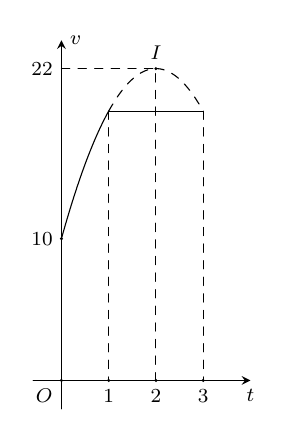
\begin{tikzpicture}[scale=0.6,font=\footnotesize,line join=round,line cap=round,>=stealth,x=1cm,y=0.3cm]
			\def\a{-3} \def\b{12}  \def\c{10}
			\def\xt{-0.6}  \def\xp{4} \def\yt{24} \def\yd{-2}
			\draw[->] (\xt,0)--(\xp,0)  node [below]{$t$};
			\draw[->] (0,\yd)--(0,\yt) node [right]{$v$}; 
			\node at (0,0)  [below left]{$O$};
			\clip (\xt-0.1,\yd+0.1)  rectangle (\xp-0.1,\yt-0.1);
			 \draw[smooth,samples=300] plot[domain=0:1](\x,{\a*(\x)^2+\b*(\x)+\c});
			\draw[smooth,samples=300,dashed] plot[domain=1:3](\x,{\a*(\x)^2+\b*(\x)+\c}); 
			\draw[dashed] (0,22)  node[left]{$22$}--(2,22)--(2,0) node[below]{$2$};
			\draw[dashed]  (3,19)--(3,0) node[below]{$3$};
			\draw[dashed] (1,19)--(1,0) node[below]{$1$}; 
			\draw (1,19)--(3,19); 
			\node at (0,10) [left]{$10$}; 
			\node  at (2,22) [above]{$I$};
			\fill  (0,0) circle (1pt)
				(0,10) circle (1pt) 
				(1,0) circle  (1pt)
				(2,0)  circle (1pt)
				(3,0) circle  (1pt)
				(2,22)  circle (1pt);
		\end{tikzpicture}
	 }
	\shortans{53} 
	\loigiai{ 
		Gọi phương trình chuyển động của vật trong $1$ giờ đầu là $v(t)=at^2+bt+c$.\\ 
		Từ đồ thị ta có 
		 $\heva{&v(0)=10\\&v(2)=22\\&\dfrac{-b}{2a}=2}
		 \Leftrightarrow
		 \heva{&c=10\\&4a+2b+c=22\\&4a+b=0}
		\Leftrightarrow 
		\heva{&a=-3\\&b=12\\&c=10.}$\\ 
		Suy ra  $v(t)=-3t^2+12t+10$.\\
		Quãng  đường đi được trong giờ đầu là $S_1=\displaystyle\int_0^1(-3t^2+12t+10)\mathrm{\,d}t=15$ (km).\\
		Tại thời điểm $t=1$, vận tốc  của vật là $v(1)=19$ (km/h).\\
		Quãng đường vật đi được trong $2$ giờ tiếp theo  là $S_2=19\cdot2=38$ (km).\\
		Quãng đường vật đi được trong $3$ giờ là  $S=S_1+S_2=53$ (km).
	} 
\end{bt}

% nguồn: Phan2_Lop_12_Dai_so_Chuong_4
\begin{bt}%[2D4V2-6]%[ma:b5403b05]
	Hệ thống lọc nước bể bơi vô cùng quan trọng khi tiến hành xây dựng công trình bơi lội để nguồn nước được làm sạch thường xuyên và giữ vệ sinh cho người bơi. Trong quá trình vận hành lọc nước thì lượng nước trong bể sẽ thay đổi theo thời gian. Lượng nước trong bể giảm nếu hệ thống đang xả nước bẩn ra khỏi bể và tăng nếu hệ thống đang cấp thêm nước sạch cho bể. Biết rằng $1$ gallon gần bằng $3{,}785$ lít, dung tích của bể là $1000$ gallon, vào thời điểm $6$ giờ sáng bể chứa $250$ gallon nước. Hàm số $f(t)$ biểu thị cho tốc độ thay đổi lượng nước trong bể theo thời gian $t$ giờ, từ thời điểm $6$ giờ sáng đến $6$ giờ chiều được cho bởi $$f(t)=\left\{\begin{aligned}
	&100t \text{ khi }0\le t\le 3\\ &900-200t \text{ khi }3\le  t\le 6\\ &100t-900 \text{ khi }6\le t\le 12
\end{aligned}
\right.$$ với  mốc thời gian $t=0$ tại thời điểm $6$ giờ sáng. Hỏi ở thời điểm $6$ giờ chiều thì trong bể chứa nhiêu gallon nước?
\shortans{700} 
\loigiai{Gọi $F(t)$ là một  nguyên hàm của hàm số $f(t)$.\\
	Vì $f(t)$ biểu thị cho tốc độ thay đổi lượng nước trong bể theo  thời gian $t$ nên $F(t)$ chính là lượng nước có trong bể theo thời gian $t$.\\
	Lượng nước trong bể lúc $6$ giờ sáng (ứng với $t=0$) là  $F(0)=250$.\\
	Lượng nước trong bể lúc $6$ giờ chiều (ứng với $t=12$) là $F(12)$.\\  Ta có $\displaystyle\int^{12}_0 f(t)\, \mathrm{d}t=F(12)-F(0)\Rightarrow F(12)=F(0)+\displaystyle\int^{12}_0 f(t)\,\mathrm{d}t$.\\
	Nên $F(12)=250 + \displaystyle\int^3_0100t\ \mathrm{d}t +\displaystyle\int^6_3(900-200t)\,  \mathrm{d}t +\displaystyle\int^{12}_6(100t-900)\, \mathrm{d}t=700$ gallon.
} 
\end{bt}

% nguồn: Phan2_Lop_12_Dai_so_Chuong_4
\begin{bt}%[2D4V2-6]%[ma:7359a405]
	\immini[thm]{Một khinh khí cầu thay đổi vận tốc lên cao $v(t)$ theo biểu đồ bên. Nó khởi hành ở độ cao $350$ (mét) so với mực nước biển. Hỏi sau  $200$ (giây), khinh khí cầu ở độ cao bao nhiêu mét so với mực nước biển?}{
	\begin{tikzpicture}[line join=round,line cap=round,>=stealth,font=\footnotesize,scale=1]
			 \tikzset{
				khicau/.pic={ 
			 \fill[yellow!15] (4.391,10.304)
				..  controls (-0.128,10.257) and (-0.011,6.648).. (2.353,3.877)
				.. controls (2.676,3.495)  and (3.045,3.121).. (3.46,2.759)
				.. controls (4.391,2.761) and (4.391,2.76)..  (5.321,2.76)
				.. controls  (5.732,3.119) and (6.101,3.493).. (6.424,3.871)
				.. controls (8.788,6.646) and (8.92,10.252).. (4.39,10.304); 
			\fill[cyan!40] (0.906,8.517) 
				.. controls (0.96,8.565) and (1.119,8.601)..  (1.174,8.576)
				 .. controls (1.365,8.696) and (1.55,8.74).. (1.797,8.68)
				.. controls (1.909,8.794) and (2.294,8.834)..  (2.67,8.774)
				.. controls (3.093,8.962) and  (3.52,8.962).. (3.888,8.88)
				.. controls (4.047,8.943) and (4.586,8.968)..  (4.905,8.844)
				.. controls (5.306,8.986) and (5.747,8.932)..  (6.102,8.801)
				 .. controls (6.537,8.877) and (6.773,8.875).. (6.969,8.728)
				 .. controls (7.24,8.82) and (7.457,8.754).. (7.585,8.63)
				 .. controls (7.631,8.655) and (7.758,8.661).. (7.823,8.639)
				.. controls  (7.729,8.856) and (7.617,9.015).. (7.483,9.179)
				.. controls (7.418,9.21) and  (7.344,9.222).. (7.254,9.177)
				.. controls (7.086,9.306) and (6.908,9.336)..  (6.669,9.272)
				.. controls (6.378,9.434)  and (6.1,9.431).. (5.823,9.333)
				.. controls (5.468,9.482)  and (5.094,9.549).. (4.756,9.421)
				 .. controls (4.565,9.524) and (4.215,9.52).. (4.031,9.427)
				.. controls (3.734,9.544) and  (3.272,9.526).. (2.995,9.384)
				.. controls (2.681,9.437) and  (2.331,9.374).. (2.096,9.25)
				.. controls (1.879,9.294) and  (1.664,9.253).. (1.494,9.138)
				.. controls (1.433,9.159) and (1.298,9.146)..  (1.228,9.092)
				.. controls  (1.087,8.902) and (0.98,8.716).. (0.906,8.516);
			 \fill[orange!40] (0.906,8.517)
				 .. controls (0.96,8.565) and (1.119,8.601).. (1.174,8.576)
				..  controls (1.365,8.696) and (1.55,8.74).. (1.797,8.68)
				.. controls (1.909,8.794)  and (2.294,8.834).. (2.67,8.774)
				.. controls (3.093,8.962)  and (3.52,8.962).. (3.888,8.88)
				..  controls (4.047,8.943) and (4.586,8.968).. (4.905,8.844)
				 .. controls (5.306,8.986) and (5.747,8.932).. (6.102,8.801)
				.. controls (6.537,8.877)  and (6.773,8.875).. (6.969,8.728)
				.. controls (7.24,8.82) and (7.457,8.754)..  (7.585,8.63)
				.. controls (7.631,8.655) and (7.758,8.661).. (7.823,8.639) 
				.. controls  (7.908,8.467) and (7.989,8.169).. (8.014,7.99)
				..  controls (7.946,8.016) and (7.846,8.044).. (7.751,8.003)
				.. controls (7.635,8.127) and  (7.344,8.171).. (7.121,8.109)
				.. controls (6.88,8.224) and (6.56,8.26)..  (6.247,8.187)
				.. controls (5.92,8.313) and (5.402,8.325).. (5.002,8.209) 
				.. controls (4.741,8.33) and (4.084,8.322)..  (3.779,8.202)
				 .. controls (3.358,8.276) and (2.869,8.262).. (2.526,8.12)
				.. controls (2.158,8.183) and (1.886,8.142).. (1.653,8.021) 
				.. controls (1.408,8.061) and (1.184,8.016)..  (1.016,7.902)
				.. controls (0.924,7.92) and (0.819,7.903)..  (0.75,7.869)
				..  controls (0.778,8.128) and (0.817,8.282).. (0.906,8.516);
			 \fill[cyan!30] (1.977,4.347)
				.. controls (2.04,4.311) and  (2.183,4.304).. (2.262,4.342)
				.. controls (2.411,4.302) and  (2.64,4.261).. (2.778,4.344)
				.. controls  (2.952,4.242) and (3.158,4.275).. (3.421,4.361)
				.. controls (3.648,4.275) and (3.766,4.309)..  (4.02,4.417)
				.. controls  (4.304,4.278) and (4.52,4.306).. (4.762,4.437)
				..  controls (5.018,4.302) and (5.162,4.274).. (5.387,4.422)
				.. controls (5.63,4.305) and (5.894,4.302).. (6.045,4.406) 
				.. controls (6.23,4.283)  and (6.384,4.292).. (6.519,4.343)
				..  controls (6.565,4.286) and (6.718,4.29).. (6.777,4.312)
				.. controls (6.919,4.502) and  (6.988,4.612).. (7.118,4.801)
				.. controls (7.033,4.789) and (6.922,4.804).. (6.856,4.855) 
				 .. controls (6.717,4.803) and (6.535,4.819).. (6.342,4.932)
				.. controls (6.103,4.822)  and (5.856,4.848).. (5.619,4.965)
				 .. controls (5.342,4.848) and (5.164,4.839).. (4.852,4.963)
				 .. controls (4.557,4.851) and (4.246,4.868).. (3.922,4.974)
				.. controls (3.593,4.84) and (3.404,4.862)..  (3.17,4.946)
				.. controls (2.932,4.847)  and (2.679,4.805).. (2.455,4.907)
				.. controls (2.261,4.811) and (2.079,4.775).. (1.929,4.844) 
				.. controls (1.853,4.779)  and (1.723,4.792).. (1.653,4.816)
				.. controls  (1.758,4.659) and (1.794,4.603).. (1.976,4.347);
			\fill[orange!40] (1.977,4.347) 
				.. controls  (2.04,4.311) and (2.183,4.304).. (2.262,4.342)
				..  controls (2.411,4.302) and (2.64,4.261).. (2.778,4.344)
				.. controls (2.952,4.242) and (3.158,4.275)..  (3.421,4.361)
				.. controls (3.648,4.275) and  (3.766,4.309).. (4.02,4.417)
				.. controls (4.304,4.278) and  (4.52,4.306).. (4.762,4.437)
				.. controls (5.018,4.302) and  (5.162,4.274).. (5.387,4.422)
				.. controls (5.63,4.305) and (5.894,4.302)..  (6.045,4.406)
				.. controls (6.23,4.283) and  (6.384,4.292).. (6.519,4.343)
				.. controls (6.565,4.286) and  (6.718,4.29).. (6.777,4.312)
				 .. controls (6.644,4.14) and (6.581,4.039).. (6.425,3.872)
				.. controls  (6.355,3.827) and (6.228,3.833).. (6.158,3.865)
				.. controls (6.05,3.808) and (5.862,3.809)..  (5.711,3.877)
				.. controls (5.54,3.811) and  (5.296,3.822).. (5.146,3.905)
				.. controls (4.967,3.833) and (4.826,3.815).. (4.653,3.889) 
				..  controls (4.511,3.808) and (4.277,3.814).. (4.125,3.887)
				.. controls (3.989,3.796) and (3.8,3.804)..  (3.648,3.875)
				.. controls  (3.494,3.799) and (3.238,3.804).. (3.077,3.874)
				.. controls (2.965,3.82) and  (2.742,3.824).. (2.622,3.866)
				.. controls (2.551,3.831)  and (2.456,3.823).. (2.352,3.877)
				.. controls (2.154,4.1) and (2.113,4.156)..  (1.977,4.347);
			\fill[blue!50!black] (5.32,2.76) 
				 .. controls (5.389,2.821) and (5.457,2.881).. (5.525,2.942)
				 .. controls (4.754,2.928) and (4.024,2.929).. (3.256,2.942)
				.. controls (3.324,2.881) and (3.392,2.821)..  (3.46,2.76)--cycle;
			\draw[fill=red!70!cyan]  (5.048,2.237)
				.. controls (5.1,2.413) and (5.213,2.636)..  (5.321,2.76)
				.. controls  (4.734,2.76) and (4.043,2.76).. (3.46,2.76)
				.. controls (3.563,2.646) and (3.702,2.404)..  (3.748,2.225)--cycle
				(4.084,1.094)  rectangle (4.692,1.589)
				(4.636,1.587)--(5.048,2.237) 
				 (4.152,1.588)--(3.748,2.225)
				 (4.234,1.588)--(3.917,2.227)
				(4.29,1.588)--(4.078,2.229) 
				(4.348,1.588)--(4.248,2.229) 
				(4.391,1.588)--(4.391,2.234) 
				(4.441,1.588)--(4.541,2.232) 
				 (4.497,1.588)--(4.71,2.234)
				(4.554,1.588)--(4.873,2.234); 
			 \draw (4.394,10.304).. controls (-0.129,10.254) and (-0.008,6.65).. (2.352,3.879)
				.. controls (2.676,3.496) and (3.046,3.121)..  (3.46,2.76)
				(4.394,10.305).. controls (-0.468,10.037) and  (0.465,5.778).. (3.64,2.761)
				(4.392,10.304)..  controls (1.06,10.115) and (0.571,6.86).. (3.903,2.758)
				(4.392,10.305).. controls (1.977,9.533) and  (1.84,7.077).. (4.23,2.759)
				(4.392,10.305).. controls (3.482,8.56) and (3.529,6.178).. (4.386,2.759) 
				(4.387,10.303)..  controls (5.218,8.746) and (5.331,6.532).. (4.394,2.758)
				(4.388,10.306)..  controls (6.802,9.528) and (6.933,7.075).. (4.552,2.76)
				 (4.387,10.304).. controls (7.721,10.115) and (8.214,6.861).. (4.882,2.759)
				 (4.386,10.303).. controls (9.248,10.036) and (8.311,5.779).. (5.14,2.76)
				 (4.388,10.306).. controls (8.917,10.251) and (8.79,6.647).. (6.424,3.872)
				.. controls (6.101,3.493) and (5.732,3.12).. (5.32,2.759);}} 
			\draw[step=1,gray!50,opacity=0.5] (0,-1)  grid (5,2);
			\draw[line width=1.2pt,color=red] (0,1)--(1,1)--(3,-1)--(4,0); 
			 \draw [->] (-0.5,0)--(5,0) node[below]{$t$};
			\draw  [->] (0,-1.2)--(0,2.5) node[left]{$v$};
			\pic[scale=0.3]  at (3.5,0) {khicau};
			\foreach \i/\g in {1/50,2/100,3/150,4/200}{\draw(\i,0) circle (1pt) 
				 ($(\i,0)+(-90:3mm)$) node[scale=1]{$\g$};}
			\foreach  \i/\g in {-1/-2,1/2,2/4}{\draw(0,\i) circle (1pt)
				($(0,\i)+(180:3mm)$)  node[scale=1]{$\g$};}
			\fill  (0,0) circle (1pt) node[shift=(-135:0.25)]{$O$};
		\end{tikzpicture}
	} 
	\shortans{400} 
	 \loigiai{
		Từ đồ thị, ta có ba đoạn thẳng và các tập  xác định. Do đó ta có hàm số
		 $$v(t)=\heva{
		 &2 &&\text{ khi } 0\le t \le50\\
		&-0,04t+4 &&\text{  khi } 50<t\le150\\
		 &0,04t-8 &&\text{ khi } 150 \le t \le200
		} \text{  ($v$ tính bằng m/s, $t$ tính bằng s).}$$
		Độ cao tăng thêm là tích phân xác định của  $v(t)$ trên $[0;200]$
		\begin{itemize}
			\item  $\displaystyle\int_0^{50} 2\mathrm{\,d}t=2t \bigg|_0^{50}=100 $ m.
			\item  $\displaystyle\int_{50}^{150} (-0,04t+4)\mathrm{\,d}t=\left[-0,02t^2+4t\right] \bigg|_{50}^{150}=0 $ m.
			\item $\displaystyle\int_{150}^{200} (0,04t-8)\mathrm{\,d}t=\left[0,02t^2-8t\right] \bigg|_{150}^{200}=-50 $ m. 
		\end{itemize}
		Vậy tổng mức tăng độ cao là $100+0-50=50$ m.\\ 
		Sau $200$ giây, khinh khí cầu ở độ cao  $350+50=400$ m so với mực nước biển.
	} 
\end{bt}

% nguồn: Phan2_Lop_12_Dai_so_Chuong_4
\begin{bt}%[2D4V2-6]%[ma:262a3bf1]
	Tốc độ $v$ km/phút của một ca nô cao  tốc thay đổi theo thời gian $t$ (phút) như đồ thị ở hình vẽ sau
	\begin{center}
		\begin{tikzpicture}
				\def\xmax{11} 
				\def\ymax{1.7} 
				\draw[->] (0,-\ymax*0.05)  -- (0,\ymax*1.05) node[above] {$v$};
				\draw[->] (-\xmax*0.02,0)  -- (\xmax*1.02,0) node[right] {$t \text{ (phút)}$};
				\node at (0,0) [below left]  {O};
				\node at (0,\ymax*0.95) [above left]  {(\text{km/phút})};
				\draw  (0,0)--(2,1.2)--(7,1.2)--(10,0) node[below]{$20$};
				\draw[dashed] (0,1.2) node[left]{$1,2$}--(2,1.2)--(2,0)  node[below]{$2$}
					(7,1.2)--(7,0) node[below]{$16$}; 
			\end{tikzpicture}
	\end{center}
	Tính tốc độ trung bình của cano trong khoảng thời gian $20$  phút đầu tiên.
	 \shortans{1,02}
	 \loigiai{
		Từ đồ thị, ta có tốc độ của ca nô được  tính theo công thức:
		$v(t)=\heva{&0{,}6t &&&&\text{ khi }0\le t<2 \\&1{,}2 &&&&\text{ khi }2\le  t<16 \\&6-0{,}3t &&&&\text{ khi }16\le t\le 20.}$\\
		Quãng  đường cano di chuyển được trong $20$ phút đầu tiên là
		\begin{eqnarray*}
			 \displaystyle s&=&\int_0^2 0{,}6t\mathrm{\,d}t+\int_2^{16}1{,}2\mathrm{\,d}t+\int_{16}^{20}\left(6-0{,}3t\right)\mathrm{\,d}t \\
			&=&\dfrac{6}{5}+\dfrac{84}{5}+\dfrac{12}{5}=\dfrac{102}{5} \text{ (km).} 
		\end{eqnarray*}
		Tốc độ trung bình của  cano trong $20$ phút đầu tiên là $$v_{tb}=\dfrac{s}{20}=\dfrac{102}{100}=1{,}02 \,\,\text{ (km/phút).}$$
	} 
\end{bt}

% nguồn: Phan2_Lop_12_Dai_so_Chuong_4
\begin{bt}%[2D4V2-6]%[ma:26f123c1]
	Ông An  có một cái bình đựng rượu, thân bình có hai phần: phần phía dưới là hình nón cụt, phần trên là hình cầu bị cắt bỏ 2 đầu chỏm (hình 1). Thiết diện qua trục của bình như hình 2.
	Biết $AB=CD=16$ cm, $EF=30$ cm, $h=12$ cm, $h'=30$ cm và giá mỗi lít rượu là $100\,000$ đồng. Hỏi  số tiền ông An cần để đổ đầy bình rượu là bao nhiêu triệu đồng (giả sử độ dày của vỏ bình rượu không đáng kể)? (làm tròn kết quả đến hàng phần trăm)
	 \shortans{1,62}
	\loigiai{ 
		\begin{center}
			\begin{tikzpicture}[scale=0.18,line join=round,line cap=round,>=stealth,blue]
					\coordinate  (C) at (0,0);
					 \coordinate (D) at (14,0);
					 \coordinate (I) at (7,17);
					\coordinate (A) at  (0,14);
					\coordinate (B) at  (14,14);
					\coordinate (E) at (-10,-30); 
					\coordinate (F) at (24,-30); 
					\coordinate (K) at  ($(A)!0.5!(B)$);
					\coordinate  (O) at ($(C)!0.5!(B)$);
					 \draw (D) arc (-45:225:10);
					\draw  (C)--(E)--(F)--(D)--cycle;
					\draw (I)--(O); 
					\draw  (C)--(B)--(A)
						(B)--(D); 
					\draw[->]  (25,-30)--(25,10);
					\draw[dashed]  (D)--(25,0);
					\draw [<->]  (25,-30)--(25,0) node[midway,right]{30};
					\draw[<->] (25,0)--(25,10)  node[right,midway]{12};
					\node[right] at  (B){$B$};
					\node[above]  at (I){$I$};
					\node[left]  at (A){$A$};
					\node[left]  at (C){$C$};
					\node[below  right] at (D){$D$};
					\node[below left] at (E){$E$}; 
					\node[below right] at (F){$F$}; 
					\node[right]  at (O){$O$};
					 \node[above left] at (K){$K$};
				\end{tikzpicture}
		\end{center}
		Ta  có $CB=\sqrt{CD^2+DB^2}=20$.\\
		Gọi $O$,  $K$, $I$ lần lượt là tâm mặt cầu, trung điểm của cạnh $AB$ và cung $AB$.\\
		Ta có bán kính mặt cầu $R=\dfrac{CB}{2}=10$,  $IK=4$.\\
		Thể tích khối nón cụt $V_1=\dfrac{1}{3}\pi \cdot 30\cdot(15^2+15 \cdot  8+8^2)=4\,090\pi$.\\
		Thể tích khối cầu: $V_c=\dfrac{4\,000\pi}{3}$.\\ 
		Thể tích chỏm cầu: $V'=2\cdot\pi\cdot 16\left(10-\dfrac{4}{3}\right)=\dfrac{832\pi}{3}$.\\ 
		Thể tích bình rượu  bằng
		 \[V=V_1+V_c-V'=4\,090\pi+\dfrac{4\,000\pi}{3}-\dfrac{832\pi}{3}=\dfrac{15\,438\pi}{3} \approx 16\,166{,}64(\text{cm}^3) \approx 16{,}2.\]
	Vậy, số tiền ông An  cần để đổ đầy bình rượu gần bằng: $16{,}2\cdot 0{,}1=1{,}62$ (triệu đồng).}
\end{bt}

% nguồn: Phan2_Lop_12_Dai_so_Chuong_4
\begin{bt}%[2D4V2-6]%[ma:6360e014]
	Một ô tô bắt đầu chuyển động nhanh dần đều với vận tốc $v_1(t)=2t$ (m/s). Đi được $12$ giây, người lái xe gặp chướng ngại vật và phanh gấp, ô tô tiếp tục chuyển động chậm dần đều  với gia tốc $a=-12$ (m/s$^2$). Tính quãng đường $s$ (m) đi được của ô tô từ lúc bắt đầu chuyển động đến khi dừng hẳn.
	\shortans{168} 
	 \loigiai{
		\textbf{Giai đoạn 1:} Xe bắt đầu chuyển  động đến khi gặp chướng ngại vật.\\
		Quãng đường xe đi được là $S_1 = \displaystyle\int_0^{12} v_1(t)  \mathrm{\,d}t = \displaystyle\int_0^{12} 2t \mathrm{\,d}t = t^2\Big|_0^{12} = 144$ (m).\\
		\textbf{Giai đoạn 2:} Xe  gặp chướng ngại vật đến khi dừng hẳn.\\
		Ô tô  chuyển động chậm dần đều với vận tốc $v_2(t) = \displaystyle\int a \mathrm{\,d}t = -12t + c$.\\
		Vận tốc của xe khi gặp chướng ngại vật là $v_2(0) = v_1(12) = 2\cdot 12 =  24$ (m/s).\\
		Suy ra $-12\cdot 0 + c = 24 \Rightarrow c =  24$.\\
		Do đó $v_2(t) = -12t +  24$.\\
		Thời gian khi  xe gặp chướng ngại vật đến khi xe dừng hẳn là nghiệm phương trình
		\[-12t + 24 = 0 \Rightarrow  t = 2.\]
		Khi đó, quãng đường xe  đi được là
		\[S_2 = \displaystyle\int_0^{2} v_2(t) \mathrm{\,d}t = \displaystyle\int_0^{2} (-12t + 24) \mathrm{\,d}t = (-6t^2 + 24t)\Big|_0^2 =  24\,\text{ (m)}.\]
		Vậy tổng quãng đường xe đi được là $S = S_1 + S_2  = 168$ (m).
	} 
\end{bt}

% nguồn: Phan2_Lop_12_Dai_so_Chuong_4
\begin{bt}%[2D4V2-6]%[ma:18d863e1]
	Một bác  thợ xây bơm nước vào bể chứa nước. Gọi $h(t)$ là thể tích nước bơm được sau $t$ giây.
	Cho $h'(t) = 3at^2 + bt$ (m$^3$/s) và ban đầu bể không có nước. Sau $5$ giây thì thể tích nước trong bể là $150$ m$^3$. Sau  $10$ giây thì thể tích nước trong bể là $1\,100$ m$^3$. Hỏi thể tích nước trong bể là bao nhiêu m$^3$ sau khi bơm được $20$ giây?
	\shortans{8400} 
	\loigiai{ 
		Ta có $h'(t) =  3at^2 + bt \Rightarrow h(t)=\displaystyle\int \left(3at^2+bt\right)\mathrm{\,d}t = at^3 + \dfrac{1}{2}bt^2 + C \Rightarrow h(t) = at^3+\dfrac{1}{2}bt^2 + C$.\\
		Chọn $t = 0 \Rightarrow h(0)=0 \Rightarrow C =  0 \Rightarrow h(t) = at^3+\dfrac{1}{2}bt^2$.\\
		Sau $5$ giây thì thể tích nước trong bể là $150$ m$^3$ hay $$h(5) = 150  \Leftrightarrow 125a + \dfrac{25}{2}b = 150.$$
		Sau $10$ giây thì thể tích nước trong bể là $1\,100$ m$^3$ hay $$h(10) = 1\,100  \Leftrightarrow 1\,000a + 50b = 1\,100.$$
		Ta có hệ phương  trình
		\begin{eqnarray*}
			&&\heva{&125a + \dfrac{25}{2}b = 150\\ &1\,000a + 50b =  1\,100}\\
			&\Leftrightarrow&\heva{&a = 1\\ &b  = 2.}
		\end{eqnarray*}
		 Suy ra $h(t)=t^3+t^2$.\\
		Vậy thể tích nước trong bể sau khi bơm  được $20$ giây là $h(20)=20^3+20^2=8\,400$ m$^3$.
	 }
\end{bt}

% nguồn: Phan2_Lop_12_Dai_so_Chuong_4
\begin{bt}%[2D4V2-6]%[ma:48416f94]
	Vận tốc (dặm/giờ) của một máy bay khi bay ngược chiều gió được cho bởi công thức $v(t)=30(16-t^2)$ với $0 \le t \le 3$. Khi  vận tốc tức thời đạt $400$ dặm/giờ thì máy bay đã đi được quãng đường bao xa kể từ thời điểm bay ngược chiều gió (kết quả làm tròn đến hàng đơn vị của dặm)?
	 \shortans{740}
	\loigiai{Ta có $s(t) = \displaystyle\int_{0}^{t}30(16-t^2)\mathrm{d}t = 480t  - 10t^3$.\\
		Khi vận tốc tức thời đạt $400$ dặm/giờ tức là $30(16-t^2) = 400 \Leftrightarrow t = \dfrac{\sqrt{24}}{3}$ (giờ).\\ 
		Khi đó máy bay  đã bay được quãng đường là
	\[s =  480 \cdot \dfrac{\sqrt{24}}{3} - 10 \left(\dfrac{\sqrt{24}}{3}\right)^3 \approx 740 \text{ (dặm)}.\]}
\end{bt}

% nguồn: Phan2_Lop_12_Dai_so_Chuong_4
\begin{bt}%[2D4V2-6]%[ma:0a13825c]
	Một bồn chứa nước bị rò rỉ với tốc độ  nước chảy vào thời điểm $t$ phút được cho bởi công thức $V'(t)=160-2t$ (lít/phút). Biết rằng $V(t)$ (tính bằng lít) là thể tích nước trong bồn tại thời điểm $t$ phút. Thể tích nước chảy khỏi bồn trong $15$ phút đầu tiên kể từ khi nước bị rò rỉ bằng \ldots lít.
	 \shortans{2175}
	 \loigiai{
		$V=\displaystyle \int_{0}^{15} V'(t) \mathrm{\,d}t = \int_{0}^{15} (160-2t) \mathrm{\,d}t = \left(160t-t^2\right)\bigg|_{0}^{15} = 2\,175$.\\ 
		Vậy thể tích nước chảy khỏi bồn trong  $15$ phút đầu tiên kể từ khi nước bị rò rỉ bằng $2\,175$ lít.
	} 
\end{bt}

% nguồn: Phan2_Lop_12_Dai_so_Chuong_4
\begin{bt}%[2D4V2-6]%[ma:20df82e5]
	Doanh thu bán hàng của một doanh nghiệp khi bán một loại sản phẩm là số tiền ${R(x)}$ (triệu đồng) thu được khi $x$ đơn vị sản phẩm được bán ra. Tốc độ biến động (thay đổi) của doanh thu khi $x$ đơn vị sản phẩm đã được bán là hàm số $M_R(x)=R'(x)$. Đại diện của doanh nghiệp cho biết tốc độ biến đổi của doanh thu khi bán  một loại sản phẩm được cho bởi $M_R(x)=500 - 0{,}1x$ ở đó $x$ là số lượng sản phẩm đã bán. Hỏi doanh thu của doanh nghiệp khi đã bán $2\,000$ sản phẩm là bao nhiêu nghìn triệu đồng?
	 \shortans{800}
	 \loigiai{
		Doanh thu của doanh nghiệp là $$R(x) = \displaystyle\int M_R(x)\mathrm{\,d}x = \displaystyle\int \left( 500-0{,}1x\right)\mathrm{\,d}x=500x-\dfrac{1}{20}{x^2} + C.$$ 
		Vì $R(0) = 0$ nên $C  = 0$. Suy ra $R(x) = 500x - \dfrac{1}{20}{x^2}$.\\
		Vậy doanh  thu của doanh nghiệp khi bán $2\,000$ sản phẩm là $$R(2\,000) = 500\cdot 2\,000 - \dfrac{1}{20}\cdot 2\,000^2 = 800\,000 \, \text{ (triệu đồng)}.$$
	 }
\end{bt}

% nguồn: Phan2_Lop_12_Dai_so_Chuong_4
\begin{bt}%[2D4V2-6]%[ma:f89d15f7]
	Cường độ dòng điện trong một dây dẫn tại thời điểm $t$ giây là  $I(t)=Q'(t)=3t^2-6t+5$ với $Q(t)$ là điện lượng truyền trong dây dẫn tại thời điểm $t$. Biết rằng khi $t=1$ giây, điện lượng truyền trong dây dẫn là $Q(1)=4$. Tính điện lượng truyền trong dây dẫn khi $t=3$.
	\shortans{16} 
	\loigiai{ 
		Ta  có: $Q(t)=\displaystyle\int Q'(t))\mathrm{\,d}t=\displaystyle\int \left(3t^2-6t+5 \right)\mathrm{\,d}t =t^3-3t^2+5t+C$.\\
		 vì $Q(1)=4\Rightarrow C=1\Rightarrow Q(t)=t^3-3t^2+5t+1\Rightarrow Q(3)=16.$
	 }
\end{bt}

% nguồn: Phan2_Lop_12_Dai_so_Chuong_4
\begin{bt}%[2D4V2-6]%[ma:5fe5f829]
	Một xe ô tô đang chạy với tốc độ $72$ km/h thì người lái xe bất ngờ phát hiện chướng ngại vật trên đường cách đó $55$ m. Người lái xe, phản ứng mất $1$ giây sau đó rồi đạp phanh. Kể từ thời điểm này, ô tô chuyển  động chậm dần đều với tốc độ $v(t)=-10 t+20$ (m/s), trong đó $t$ là thời gian tính bằng giây kể từ lúc đạp phanh. Khi xe ô tô dừng hẳn, khoảng cách từ ô tô đến chướng ngại vật là bao nhiêu mét?
	\shortans{15} 
	\loigiai{ 
		Ta có $72$ km/h $= 20$  m/s.\\
		Quãng đường ô tô  đi được $1$ giây trước khi đạp phanh là $20\cdot 1=20$ m.\\
		Khi xe dừng hẳn  ta có $v(t)=-10t+20=0\Leftrightarrow t=2$ m.\\
		Quãng đường ô tô đi được kể từ khi đạp phanh đến khi dừng hẳn là $$\displaystyle\int_{0}^{2}\left(-10t+20\right)  \mathrm{\,d}t=20\,\mathrm{m}.$$\\
		Tổng quãng đường ô tô đi được kể từ khi phát hiện chướng ngại vật đến  khi dừng hẳn là $20+20=40$ m.\\
		Khi ô tô  dừng hẳn, khoảng cách từ ô đến chướng ngại vật là $55-40=15$ m.
	 }
\end{bt}

% nguồn: Phan2_Lop_12_Dai_so_Chuong_4
\begin{bt}%[2D4V2-6]%[ma:e8413db0]
	\immini 
	{Nhà bác Ba có tất cả $8$ cánh cửa sắt hình chữ nhật với chiều dài $2$ m và chiều rộng $1$ m. Hai mặt của mỗi cánh cửa được thiết kế như hình vẽ dưới đây. Trong đó, phần được tô đậm được sơn màu xanh, phần còn lại được sơn màu trắng. Mỗi phần sơn màu trắng  có đường biên cong là một phần của parabol có đỉnh nằm trên cạnh của hình chữ nhật. Biết rằng chi phí để sơn màu xanh là $120$ nghìn đồng/m$^2$ và chi phí sơn màu trắng là $110$ nghìn đồng/m$^2$. Hỏi, để sơn toàn bộ số cửa sắt trên, bác Ba phải tốn bao~nhiêu triệu đồng (làm tròn kết quả đến hàng phần trăm theo đơn vị triệu đồng)?
	\shortans{3,63} 
	}{\begin{tikzpicture}[line cap=round,line join=round,>=stealth,x=2cm]
		\draw[pattern=north east lines,pattern color=cyan!20](-1,0)--plot[domain=-1:0] (\x,{4*(\x+1)^2})--plot[domain=0:1] (\x,{4*(\x-1)^2})--(1,0)--plot[domain=1:0]  (\x,{-4*(\x-1)^2})--plot[domain=0:-1] (\x,{-4*(\x+1)^2})--(-1,0);
		\draw (-1,4) rectangle (1,-4) 
			(0,0)  node[below left]{$O$};
	\end{tikzpicture}
	 }
	 \loigiai{
	\immini 
		{Xét diện tích phần son  màu xanh của một phần tư cánh cửa.\\
		Chọn hệ trục tọa độ như hình vẽ. Đường biên cong là parabol có  dạng $y=ax^2(a\neq0)$.\\
		Do parabol đi qua  điểm $\left(\dfrac{1}{2};1\right)$ nên ta có $1=\dfrac{1}{4}a\Rightarrow a=4$.\\
		Vậy parabol  là $y=4x^2$.\\
		Diện tích hình phẳng giới hạn  bởi parabol $y=4x^2$, trục hoành và hai đường thẳng $x=0,x=\dfrac{1}{2}$ là $\displaystyle\int_0^{\tfrac{1}{2}}4x^2\mathrm{\,d}x=\left.\dfrac{4}{3}x^3\right|_0^{\tfrac{1}{2}}=\dfrac{1}{6}$.
		}{\begin{tikzpicture}[line cap=round,line join=round,>=stealth,x=2cm]
		\draw  plot[domain=-1:1] (\x,{4*(\x)^2});
		 \draw[->](-1,0)--(1,0) node[below]{$x$};
		\draw[->](0,-1)--(0,4)  node[left]{$y$};
		 \draw[dashed](0.5,0) node[below]{$0{,}5$}--(0.5,1)--(0,1);
	\end{tikzpicture}}
		Khi đó, phần được sơn màu xanh của 1 mặt cửa có diện tích là  $4\cdot \dfrac{1}{6}=\dfrac{2}{3}\left(\mathrm{~m}^2\right)$, còn phần diện tích được sơn màu trắng là $2\cdot 1-\dfrac{2}{3}=\dfrac{4}{3}$ m$^2$.\\
		Chi phí để sơn một cánh cửa là $2\cdot \left(120\cdot  \dfrac{2}{3}+110\cdot \dfrac{4}{3}\right)=\dfrac{1\,360}{3}$ (nghìn đồng).\\
		Chi phí để sơn 8 cánh cửa là $8\cdot \dfrac{1\,360}{3}=\dfrac{10\,880}{3}$ (nghìn  đồng) $\approx3{,}63$ (triệu đồng).
	 }
\end{bt}

% nguồn: Phan2_Lop_12_Dai_so_Chuong_4
\begin{bt}%[2D4V2-6]%[ma:9590fcd3]
	Nhiệt độ trung bình của Trái Đất có xu hướng tăng do nồng độ khí $CO_2$  trong khí quyển. Giả sử lượng $CO_2$ trong khí quyển (tính bằng ppm-parts per million) được mô tả bởi công thức $C(t)=200+20t-2t^2$, trong đó $t$ được tính theo năm, $t=0$ ứng với năm $2\,025$.
	Mối quan hệ giữa nhiệt độ trung bình của Trái Đất $T(t)$ (tính bằng $^\circ C$) và nồng độ $CO_2$ được mô tả bởi công thức $T(t)=\displaystyle\int_0^t kC(x)\mathrm{\,d}x$ với hằng số $k=0{,}005$ (mức độ ảnh hưởng của $CO_2$ lên nhiệt độ). Nếu không có biện pháp giảm phát thải khí $CO_2$, nhiệt độ trung bình của  Trái Đất có thể tăng thêm bao nhiêu $^\circ C$ từ năm $2\,025$ đến năm $2\,040$?
	\shortans{15} 
	 \loigiai{
		Sự thay  đổi của nhiệt độ trung bình của Trái Đất từ năm $2\,025$ đến năm $2\,040$ là
		$$T=0{,}005 \displaystyle\int_0^{15}  (200+20t-2t^2)\mathrm{\,d}t=15.$$
		Nếu không có biện pháp giảm phát thải khí $CO_2$, nhiệt độ trung bình của Trái  Đất có thể tăng thêm khoảng $15^\circ C$ từ năm $2\,025$ đến năm $2\,040$.
	} 
\end{bt}

% nguồn: Phan2_Lop_12_Dai_so_Chuong_4
\begin{bt}%[2D4V2-6]%[ma:705e67d7]
	Đơn đặt hàng của nhà máy cho một loại máy điều hoà không khí là khoảng $6\,000$ chiếc mỗi tuần khi giá là  $331$ USD/chiếc và khoảng $8\,000$ chiếc mỗi tuần khi giá là $303$ USD/chiếc. Hàm cung được cho bởi $p=0{,}0275x$, trong đó $x$ là số lượng máy điều hoà được bán với giá $p$ USD một chiếc. Tổng thặng dư tiêu dùng và thặng dư sản xuất bằng bao nhiêu nghìn USD (giả sử hàm cầu là hàm bậc nhất).
	 \shortans{2075}
	\loigiai{ 
		Hàm cầu  có dạng $p=ax+b$. Do đơn đặt hàng của nhà máy cho một loại máy điều hoà không khí là $6\,000$ chiếc mỗi tuần khi giá là $331$ USD/chiếc và $8\,000$ chiếc mỗi tuần khi giá là $303$ USD/chiếc nên ta có
		$$ \heva{&331=6\,000a+b \\ &303=8\,000a+b} \Leftrightarrow  \heva{&a=-0{,}014 \\ &b=415.} $$
		Vậy  hàm cầu là $p=-0{,}014x+415$.\\
		Xét phương trình $-0{,}014x+415=0{,}0275x  \Leftrightarrow x=10\,000$, khi đó $p=275$.\\
		Thặng dư tiêu dùng là 
		$$ \displaystyle\int_{0}^{10\,000}(-0{,}014x+415-275)\mathrm{d}x = 700\,000 \text{ (USD).} $$ 
		Thặng dư  sản xuất là
		$$ \displaystyle\int_{0}^{10\,000}(275-0{,}0275x)\mathrm{d}x  = 1\,375\,000 \text{ (USD).} $$
		Tổng thặng dư tiêu dùng và thặng  dư sản xuất bằng $2\,075\,000$ USD.
	} 
\end{bt}

% nguồn: Phan2_Lop_12_Dai_so_Chuong_4
\begin{bt}%[2D4V2-6]%[ma:0b0ea7e3]
	Qua điều tra các nhà phân tích kinh tế đã nhận định rằng tốc độ tăng trưởng kinh tế (GDP) của một quốc gia sau $t$ năm tính từ đầu năm $2004$ là $30 + \dfrac{1}{2}\sqrt{5+t}$ tỉ USD/năm. Biết rằng  GDP của quốc gia đó vào đầu năm $2004$ là $100$ tỉ USD. Hãy dự đoán GDP của quốc gia đó vào đầu năm $2015$ bằng bao nhiêu tỉ USD (làm tròn kết quả đến hàng đơn vị).
	\shortans{438} 
	\loigiai{ 
		Nguyên hàm của $q(t)=30+\dfrac{1}{2}\sqrt{5+t}$ là hàm số $S(t)$ mô tả GDP của quốc gia  sau $t$ năm (được tính từ năm $2004$).\\
		GDP tăng thêm tính  từ năm $2004$ ($t=0$) đến đầu năm $2015$ ($t=11$) là
		$$ \displaystyle\int_{0}^{11}q(t)\mathrm{d}t = \displaystyle\int_{0}^{11}\left(30+\dfrac{1}{2}\sqrt{5+t}\right)\mathrm{d}t = \left.\left(30t+\dfrac{(5+t)^{\frac{3}{2}}}{3}\right)\right|_{0}^{11}  \approx 347{,}6 \text{ (tỉ USD)}. $$
		Như  vậy, tổng giá trị GDP tính đến đầu năm $2015$ bằng $347{,}6+100=437{,}6$ (tỉ USD).
	} 
\end{bt}

% nguồn: Phan2_Lop_12_Dai_so_Chuong_4
\begin{bt}%[2D4V2-6]%[ma:f97fa55f]
	Giả sử anh Nam nhảy dù từ một chiếc trực thăng. Vào thời điểm $19$ giây sau khi rời khỏi trực thăng, anh Nam mở chiếc dù của mình trong $2$ giây, anh Nam chạm đất sau $19$ giây kể từ lúc  bung dù. Tại thời điểm $t$ (giây), vị trí của anh Nam cách mặt đất một khoảng $h(t)$ mét và vận tốc rơi của anh Nam (tính bằng m/s) là một hàm số được cho bởi công thức
	\[v(t)=h'(t)=\heva{&-80,&&0 \le t<19\\&37 t-783,&&19 \le t<21\\&-6&\text{ khi }&21 \le t \le 40.  }\]
	Độ cao vị trí của anh Nam khi bắt đầu nhảy ra khỏi trực thăng bằng bao  nhiêu m.
	 \shortans{1720}
	 \loigiai{
		Ta có \begin{eqnarray*}
		h&=&\displaystyle\int_0^{40}\left|h'(t)\right|\mathrm{\,  d} t\\
		&=&\displaystyle\int_0^{10}|-80|\mathrm{\, d} t+\displaystyle\int_{19}^{21}|37 t-783|\mathrm{\,d} t+\displaystyle\int_{21}^{40}|-6|\mathrm{\,d} t\\ 
		&=&80  t\bigg|_0^{19}+\left(783 t-\frac{37 t^2}{2}\right)\bigg|_{19}^{21}+6 t\bigg|_{21}^{40}=1\,720.
	\end{eqnarray*}
Vậy độ  cao vị trí của anh Nam khi bắt đầu nhảy khỏi trực thăng bằng $1\,720$ m.}
\end{bt}

% nguồn: Phan2_Lop_12_Dai_so_Chuong_4
\begin{bt}%[2D4V2-6]%[ma:72440f87]
	Trên một tuyến đường thẳng có một đoạn phải đi xuyên qua một quả núi nhỏ, do đó người ta đã tạo một hằm chui để thuận tiện  cho các phương tiện giao thông di chuyển, vòm của hầm chui được đổ bê tông có dạng như hình vẽ dưới đây với $BC=8$ m; $IH=5$ m; $IK=0{,}6$ m; $AB=CD=0{,}5$ m; $HT=10$ m. Biết khi cắt vòm của hầm chui bằng mật phẳng vuông góc với trục của tuyến đường ta luôn có thiết diện là một hình phẳng được giới hạn bởi hai parabol và giao tuyến của mặt cắt với mặt đường. Hỏi cần bao nhiêu mét khối bê tông để đổ vòm của hầm chui (làm tròn kết quả đến hàng phần mười).
	\begin{center}
		\begin{tikzpicture}[line join=round,line cap=round,>=stealth]
				\tikzset{every node/.style={scale=0.7}} 
				\draw[->]  (-5.1,0)--(13,0) node[below left] {};
				\draw[->] (0,-1.1)--(0,14) node[left] {}; 
				\draw (0,0) node  [below left] {$H$};
				\begin{scope}
					 \clip (-5,-1) rectangle (14,14);
					\fill[red!40,opacity=0.6] 
						plot[domain=-4.5:4.5,samples=300] (\x,{-112/405*(\x)^2+5.6}) 
						-- plot[domain=4:-4,samples=300]  (\x,{-5/16*(\x)^2+5})
						 -- cycle;
					 \fill[gray!40,opacity=0.6]
						 plot[domain=4:-4,samples=300] (\x,{-5/16*(\x)^2+5});
					\draw[blue,samples=300,domain=-4.5:4.5,smooth,variable=\x] 
						plot (\x,{-112/405*(\x)^2+5.6}) node[right,scale=0.8]  {};
					\draw[red,samples=300,domain=-4:4,smooth,variable=\x] 
						 plot (\x,{-5/16*(\x)^2+5}) node[right,scale=0.8] {};
					\draw[dashed,blue!70!black,samples=300,domain=2.5:5,smooth,variable=\x] 
						plot  (\x,{-112/405*(\x-7)^2+5.6+7}) node[right,scale=0.8] {};
					\draw[blue!70!black,samples=300,domain=5:11.5,smooth,variable=\x] 
						plot (\x,{-112/405*(\x-7)^2+5.6+7}) node[right,scale=0.8] {}; 
					\draw[dashed,red!70!black,samples=300,domain=3:11,smooth,variable=\x] 
						plot (\x,{-5/16*(\x-7)^2+5+7})  node[right,scale=0.8] {};
				\end{scope}
				\coordinate  (A) at (-4.5,{-112/405*(-4.5)^2+5.6});
				 \coordinate (D) at (4.5,{-112/405*(4.5)^2+5.6});
				\coordinate (V1) at (-2,364/81); 
				\coordinate (A') at  ($(A)+(7,7)$);
				\coordinate (D')  at ($(D)+(7,7)$);
				 \coordinate (V1') at ($(V1)+(7,7)$);
				 \coordinate (B) at (-4,{-5/16*(-4)^2+5});
				\coordinate (C)  at (4,{-5/16*(4)^2+5});
				\coordinate (V2)  at (0,5);
				\coordinate (V3) at (0,5.6); 
				\coordinate (B')  at ($(B)+(7,7)$);
				\coordinate (C')  at ($(C)+(7,7)$);
				 \coordinate (V2') at ($(V2)+(7,7)$);
				\coordinate (H)  at (0,0);
				\coordinate (T) at  ($(H)+(7,7)$);
				\draw[gray,dashed] (A)--(A'); 
				\draw (D)--(D'); 
				\draw (V1)--(V1'); 
				\draw[gray,dashed]  (B)--(B');
				\draw[gray,dashed] (C)--(C'); 
				\draw[dashed]  (A')--(D');
				 \draw[dashed] (H)--(T);
				\node at (T)  [above right]{$T$};
				\node at (A) [below]{$A$}; 
				\node at (B) [below]{$B$}; 
				\node at  (C) [below]{$C$};
				 \node at (D) [below]{$D$};
				\node at (D)  [below]{$D$};
				\node at (V2) [below left]{$I$}; 
				\node at (V3)  [above right]{$K$};
				\foreach \p/\pos in {V1/above  left,V1'/above right,
					A/below left,A'/above  right,
					D/below right,D'/above right, 
					V2/above left,V2'/above  right,
					B/below left,B'/above right, 
					 C/below right,C'/above right}{
					\fill  (\p) circle (1.5pt);
				 }
				\fill[orange!40,opacity=0.6] 
					(V1)--plot[domain=-2:4.5,samples=300]  (\x,{-112/405*(\x)^2+5.6})
					 (D)--(D')--plot[domain=11.5:5,samples=300] (\x,{-112/405*(\x-7)^2+5.6+7})--(V1')--(V1);
			\end{tikzpicture}
	\end{center}
	\shortans{69,3} 
	\loigiai{ 
		\begin{center}
			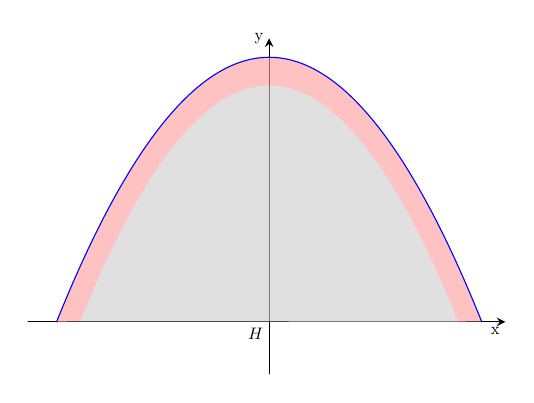
\begin{tikzpicture}[line join=round,line cap=round,>=stealth,scale=0.6]
					\tikzset{every  node/.style={scale=0.6}}
					\draw[->] (-5.1,0)--(5,0)  node[below left] {x};
					\draw[->] (0,-1.1)--(0,6) node[left]  {y};
					\draw (0,0) node [below left] {$H$}; 
					\fill[red!40,opacity=0.6] 
						plot[domain=-4.5:4.5,samples=300]  (\x,{-112/405*(\x)^2+5.6})
						 -- plot[domain=4:-4,samples=300] (\x,{-5/16*(\x)^2+5})
						--  cycle;
					\fill[gray!40,opacity=0.6] 
						 plot[domain=4:-4,samples=300] (\x,{-5/16*(\x)^2+5});
					 \draw[blue,samples=300,domain=-4.5:4.5,smooth,variable=\x]
						plot  (\x,{-112/405*(\x)^2+5.6}) node[right,scale=0.8] {};
				\end{tikzpicture}
		\end{center}
		Gọi $S$ là diện tích hình phẳng giới hạn bởi hai parabol  và giao tuyến của mặt cắt với mặt đường.\\
		Thể tích vòm của  hầm chui được đổ bê tông là $V=S \cdot HT=10S$.\\
		 Gắn phần diện tích vào hệ trục tọa độ $Oxy$, ta có đồ thị như hình vẽ.\\
		Từ đồ thị,  ta xác định được hai hàm số parabol:\\
		$g(x)=k\left(x^2-\dfrac{81}{4}\right) \xrightarrow{g(0)=\dfrac{28}{5}} k=-\dfrac{112}{405} \Rightarrow  g(x)=-\dfrac{112}{405}\left(x^2-\dfrac{81}{4}\right)$\\
		 $f(x)=h(x^2-16) \Rightarrow h=-\dfrac{5}{16} \Rightarrow f(x)=-\dfrac{5}{16}(x^2-16).$\\
		$\Rightarrow S=\displaystyle\int_{-\sqrt{3}}^{\sqrt{3}} \left(g(x)-f(x)\right) \mathrm{\,d}x=\displaystyle\int_{-\sqrt{3}}^{\sqrt{3}}  \left[-\dfrac{112}{405}\left(x^2-\dfrac{81}{4}\right)-\left(-\dfrac{5}{16}(x^2-16)\right)\right] \mathrm{\,d}x=\dfrac{104}{15}.$\\
	Vậy thể tích của vòm là \[V=\dfrac{104}{15} \cdot 10=\dfrac{208}{3} \approx  69,3(\text{m}^3).\]}
\end{bt}

% nguồn: Phan2_Lop_12_Dai_so_Chuong_4
\begin{bt}%[2D4V2-6]%[ma:a2a6b2ab]
	\immini 
	{Hai hàm  số $y = f(x)$; $y = g(x)$ đều là những hàm số bậc hai có đồ thị như hình vẽ bên cạnh. Tính diện tích phần tô đậm (\textit{làm tròn đến hai chữ số thập phân}).
	} 
	{\begin{tikzpicture}[>=stealth,line join=round,line cap=round,color=blue,font=\footnotesize,scale=0.8]
		\draw[->]  (-2,0) -- (5,0) node[below] {$x$};
		\draw[->] (0,-1)--(0,5)  node[right]{$y$};
		 \draw (0,0) node[below left]{$O$};
		\draw (-1,0)  node[above left]{$-1$}
			 (4,0) node[above right]{$4$}
			 (0,3) node[left]{$3$}
			(0,2)  node[right]{$2$};
		\fill[pattern  = north east lines,pattern color=cyan,smooth] plot[domain=-1:4] (\x,{-0.75*((\x)+1)*((\x)-4)})--plot[domain=4:-1] (\x,{-0.5*((\x)+1)*((\x)-4)})--cycle;
		\draw[violet,samples=150,smooth,domain=-1.3:4.3] plot  (\x,{-0.5*((\x)+1)*((\x)-4)});
		\draw[violet,samples=150,smooth,domain=-1.2:4.2] plot  (\x,{-0.75*((\x)+1)*((\x)-4)});
		 \draw (3.2,3.6) node[above]{\scriptsize $y = f (x)$};
		 \draw (2.45,1.4) node[above]{\scriptsize $y = g (x)$};
	\end{tikzpicture}
	} 
	 \shortans{5,21}
	 \loigiai{
		Vì hàm số  $y = f(x)$ là hàm số bậc hai và đồ thị $y = f(x)$ cắt trục $Ox$ tại các điểm có hoành độ $-1$ và $4$ nên $f(x) = a(x + 1)(x - 4)$.\\
		 Đồ thị $y = f(x)$ đi qua điểm $(0; 3)$ nên $a = -\dfrac{3}{4} \Rightarrow f(x) = -\dfrac{3}{4}(x+1)(x-4)$.\\
		Tương tự $g(x) =  -\dfrac{1}{2}(x+1)(x-4)$.\\
		Do đó diện tích phần tô đậm bằng $\displaystyle\int_{-1}^4 \left[\dfrac{-3}{4}(x+1)(x-4) + \dfrac{1}{2}(x+1)(x-4)\right] \mathrm{\,d}x = \dfrac{125}{24} \approx  5{,}21$.
	 }
\end{bt}

% nguồn: Phan2_Lop_12_Dai_so_Chuong_4
\begin{bt}%[2D4V2-6]%[ma:e6c801ed]
	Hệ thống lọc nước bể bơi vô cùng quan trọng khi tiến hành xây dựng công trình bơi lội để nguồn nước được làm sạch thường xuyên và giữ vệ sinh cho người  bơi. Trong quá trình vận hành lọc nước thì lượng nước trong bể sẽ thay đổi theo thời gian. Lượng nước trong bể giảm nếu hệ thống đang xả nước bẩn ra khỏi bể và tăng nếu hệ thống đang cấp thêm nước sạch cho bể. Biết rằng $1$ gallon gần bằng $3{,}785$ lít, dung tích của bể là $1000$ gallon và thời điểm $6$ giờ sáng bể chứa $250$ gallon nước. Hàm số $f(t)$ biểu thị cho tốc độ thay đổi lượng nước trong bể theo thời gian $t$ giờ, từ thời điểm $6$ giờ sáng đến $6$ giờ chiều được cho bởi công thức $f(t) = \heva{&100t &\text{ khi } 0 \leq t \leq 3\\&900-200t &\text{ khi } 3 \leq t \leq 6\\&100t - 900 &\text{ khi } 6 \leq t \leq 12}$ với mốc thời gian $t= 0$ tại thời điểm $6$ giờ sáng. Hỏi ở thời điểm $6$ giờ chiều thì trong bể chứa bao~nhiêu gallon nước?
	 \shortans{700}
	\loigiai{ 
		Ở thời điểm $6$ giờ chiều thì trong bể chứa số gallon nước là \begin{align*}
		 V = 250 + \displaystyle\int_0^3 100t\mathrm{\,d}t
		+ \displaystyle\int_3^6 \left(900 - 2t \right) \mathrm{\,d}t + \displaystyle\int_6^{12} \left(100t-900 \right) \mathrm{\,d}t =  700.
	\end{align*}
} 
\end{bt}

% nguồn: Phan2_Lop_12_Dai_so_Chuong_4
\begin{bt}%[2D4V2-6]%[ma:161a10fa]
	Vận tốc (dặm/giờ) của một máy bay khi bay ngược chiều gió được cho bởi công thức $v(t) = 30\left(16-t^2 \right)$ với $0\leq  t \leq 3$. Khi vận tốc tức thời đạt $400$ dặm/giờ thì máy bay đã đi qua quãng đường bao xa kể từ thời điểm bay ngược chiều gió (kết qua làm tròn đến hàng đơn vị của dặm)?
	 \shortans{740}
	 \loigiai{
		Khi  vận tốc tức thời đạt $400$ dặm/giờ tức là $30\left(16 - t^2 \right) = 400 \Leftrightarrow t = \dfrac{\sqrt{24}}{3}$ (giờ).\\
		Khi đó máy bay đã bay được quãng đường là $s(t) = \displaystyle\int^{\tfrac{\sqrt{24}}{3}}_{0} 30\left(16-t^2 \right)\mathrm{\,d}t \approx 740$ (dặm). 
	} 
\end{bt}

% nguồn: Phan2_Lop_12_Dai_so_Chuong_4
\begin{bt}%[2D4V2-6]%[ma:beb530d0]
	Một chiếc ô tô đang chạy với vận tốc $15$ m/s thì nhìn thấy chướng ngại vật trên đường cách đó $40$ m, người lái xe hãm phanh khẩn cấp. Sau khi hãm phanh, ô tô chuyển động chậm dần đều với vận tốc $v(t)=-3t+15$ (m/s), trong đó $t$ (giây) là thời gian.  Tính quãng đường xe ô tô đi được trong thời gian $t$ giây kể từ lúc đạp phanh.
	\shortans{37,5} 
	 \loigiai{
		Khi xe  dừng hẳn thì $v(t)=0\Rightarrow -3t+15=0\Rightarrow t=5$ (giây).\\
		Quãng đường xe ô tô đi được trong thời  gian $5$ (giây) là
		 $$s=\int _0^5(-3t+15)\mathrm{\,d}t=37{,}5\text{ (m)}.$$
	 }
\end{bt}

% nguồn: Phan2_Lop_12_Dai_so_Chuong_4
\begin{bt}%[2D4V2-6]%[ma:7d3f575c]
	Cho hình vẽ dưới đây là đồ thị vận tốc $v(t)$ của một vật ($t=0$ là thời điểm vật  bắt đầu chuyển động). Tính vận tốc trung bình (m/s) của vật $10$ giây đầu tiên.
	\begin{center}
		\begin{tikzpicture}[scale=1,font=\footnotesize,line join=round,line cap=round,>=stealth]
				\def\xmin{-1};  \def\ymin{-1}; \def\xmax{11}; \def\ymax{5};
				\coordinate  (O) at (0,0);
				\draw[->] (\xmin,0)--(\xmax,0) node[below]{$x$}; 
				\draw[->] (0,\ymin)--(0,\ymax) node[left]{$y$}; 
				\fill (O) node[below left]{$O$}  circle (1pt);
				 \clip ({\xmin-0.1},{\ymin-0.1}) rectangle ({\xmax+0.1},{\ymax+0.1});
				\foreach  \x in {2,4,7,10}{
					\fill (\x,0) node[below]{$\x$} circle  (1pt);
				 }
				\foreach  \y in {1,3}{
					 \fill (0,\y) node[left]{$\y$} circle (1pt);
				} 
				 \draw (0,0)--(2,1)--(4,3)--(7,3)--(10,1);
				 \draw[dashed] (2,0)|-(0,1)
					(4,0)|-(0,3) 
					 (7,0)--(7,3)
					(10,0)|-(0,1); 
			\end{tikzpicture}
	\end{center}
	\shortans{2} 
	 \loigiai{
		 Theo đồ thị ta có
		\begin{center}
			\begin{tikzpicture}[scale=1,font=\footnotesize,line join=round,line cap=round,>=stealth]
					\def\xmin{-1}; \def\ymin{-1}; \def\xmax{11};  \def\ymax{5};
					\coordinate  (O) at (0,0);
					 \draw[->] (\xmin,0)--(\xmax,0) node[below]{$x$};
					\draw[->] (0,\ymin)--(0,\ymax)  node[left]{$y$};
					\fill (O) node[below left]{$O$} circle (1pt); 
					\clip ({\xmin-0.1},{\ymin-0.1})  rectangle ({\xmax+0.1},{\ymax+0.1});
					\foreach \x in {2,4,7,10}{ 
						\fill  (\x,0) node[below]{$\x$} circle (1pt);
					 }
					\foreach \y  in {1,3}{
						\fill (0,\y) node[left]{$\y$} circle  (1pt);
					 }
					\draw (0,0)--(2,1) node[above]{$B$}--(4,3) node[above]{$C$}--(7,3) node[above]{$D$}--(10,1) node[above]{$E$}; 
					\draw[dashed] (2,0)|-(0,1) 
						 (4,0)|-(0,3)
						 (7,0)--(7,3)
						 (10,0)|-(0,1);
				\end{tikzpicture}
		\end{center}
		Phương trình đường  thẳng $O B\colon v=\dfrac{1}{2} t$.\\
		 Phương trình đường thẳng $B C\colon v=t-1$.\\
		Phương trình đường thẳng $C D\colon  v=3$.\\
		Phương trình đường  thẳng $D E\colon v=-\dfrac{2}{3} t+\dfrac{23}{3}$.\\
		Suy ra  $v(t)=\heva{&\dfrac{1}{2} t,&0\le t\le 2\\&t-1,&2<t\le 4\\&3,&4<t\le 7\\&-\dfrac{2}{3} t+\dfrac{23}{3},&7<t\le 10.}$\\
		Quãng đường chuyển động của vật  trong $10$ giây là
		\begin{eqnarray*}
			S&=&\displaystyle\int_0^{10} v(t)\mathrm{\, d}t=\displaystyle\int_0^2 v(t)\mathrm{\, d}t+\displaystyle\int_2^4 v(t)\mathrm{\, d}t+\displaystyle\int_4^7 v(t)\mathrm{\,  d}t+\displaystyle\int_7^{10} v(t)\mathrm{\, d}t\\
			S&=&\displaystyle\int_0^2 \dfrac{1}{2}  t \mathrm{\, d} t+\displaystyle\int_2^4(t-1)\mathrm{\, d}t+\displaystyle\int_4^7 3 \mathrm{\, d} t+\displaystyle\int_7^{10}\left(-\frac{2}{3} t+\frac{23}{3}\right)\mathrm{\, d}t=20.
		\end{eqnarray*}
		Vận tốc trung bình của chuyển động là $v_{\text{ tb}}=\dfrac{S}{10}=2$ (m/s). 
	} 
\end{bt}

% nguồn: Phan2_Lop_12_Dai_so_Chuong_4
\begin{bt}%[2D4V2-6]%[ma:25bddf2c]
	Sân vận động Sport Hub (Singapore) là sân có  mái vòm kỳ vĩ nhất thế giới. Đây là nơi diễn ra lễ khai mạc Đại hội thể thao Đông Nam Á được tổ chức tại Singapore năm 2015.
	Nền sân là một elip $(E)$ có trục lớn dài $150$ m, trục bé dài $90$ m. Nếu cắt sân vận động theo một mặt  phẳng vuông góc với trục lớn của $(E)$ và cắt elip ở $M$, $N$ (hình vẽ) thì ta được thiết diện luôn là một phần của hình tròn có tâm $I$ (phần tô đậm trong hình vẽ) với MN là một dây cung và góc $\widehat{MIN}=90^{\circ}$. Để lắp máy điều hòa không khí thì các kỹ sư cần tính thể tích phần không gian bên dưới mái che và bên trên mặt sân, coi như mặt sân là một mặt phẳng và thể tích vật liệu là mái không đáng kể. Thể tích tính được là bao~nhiêu (đơn vị nghìn $\mathrm{m}^3$, làm tròn đến hàng đơn vị)
	\shortans{116} 
	\loigiai{ 
		\begin{center}
			\begin{tikzpicture}[line join=round,line cap=round,>=stealth]
					\path 
						(0,0) coordinate  (O)
						 (-3,0) arc (180:60:{3cm} and {1.5cm}) coordinate (M)
						(-3,0) arc (-180:-60:{3cm} and {1.5cm}) coordinate  (N);
					 \draw
						(0,0) ellipse  (3cm and 1.5cm);
					 \draw[->]
						(-4,0)--(4,0) node[right]{$x$}; 
					 \draw[->]
						(0,-2)--(0,2)  node[above]{$y$};
					 \fill
						 (-3,0) circle (1pt)
						(3,0)  circle (1pt);
					\foreach  \i/\g in{O/-120,M/90,N/-90}
					\fill (\i) circle (1pt)  node[shift={(\g:3mm)}]{$\i$};
				\end{tikzpicture}
		\end{center}
		Chọn hệ trục $Oxy$ như hình vẽ.\\ 
		Phương trình chính tắc  của elip đáy:
		\[(E)\colon \dfrac{x^{2}}{75^{2}}+\dfrac{y^{2}}{45^{2}}=1\] 
		Gọi $M(x;y)  \Rightarrow MN=2y=2 \sqrt{45^{2}\left(1-\dfrac{x^{2}}{75^{2}}\right)}
		=90  \sqrt{1-\dfrac{x^{2}}{75^{2}}}$.\\
		 $\Rightarrow R=\dfrac{MN}{\sqrt{2}}=\dfrac{90}{\sqrt{2}} \cdot \sqrt{1-\dfrac{x^{2}}{75^{2}}}$.\\
		 Ta có công thức diện tích hình quạt:
		\[S_{\text{ quạt}}=\dfrac{\pi  R^{2}\cdot\alpha}{360^{\circ}}\]
		với $\alpha$ (theo đơn vị độ) là  số đo góc ở tâm chắn cung tương ứng.
		\begin{center}
			\begin{tikzpicture}[line join=round,line cap=round,>=stealth]
					\path 
						(0,0)  coordinate (I)
						 (45:2) coordinate (M)
						 (135:2) coordinate (N);
					\foreach \i/\g in{I/-90,M/60,N/120} 
					\fill (\i)  circle (1pt) node[shift={(\g:3mm)}]{$\i$};
				\fill[pattern=north west lines] (M) -- (N) arc[start angle=135,end angle=45,radius=2] -- cycle;
				 \draw (I) circle (2cm);
				 \draw (M)--(I) node[pos=.5,right]{$R$}--(N)--cycle;
			\end{tikzpicture}
		\end{center}
		Gọi $S(x)$ là diện tích  thiết diện, ta có
		\allowdisplaybreaks 
		\begin{eqnarray*}
			S(x)&=&S_{\text{ quạt}}-S_{\triangle  IMN}\\
			 &=&\dfrac{1}{4} \pi R^{2}-\dfrac{1}{2} R^{2}\\
			 &=&\left(\dfrac{1}{4} \pi-\dfrac{1}{2}\right)R^{2}\\
			 &=&(\pi-2)\dfrac{2025}{2}\cdot\left(1-\dfrac{x^{2}}{75^{2}}\right).
		\end{eqnarray*}
		Thể tích  khoảng không gian sân vận động là
		\[V=\displaystyle\int_{-75}^{75}(\pi-2) \dfrac{2025}{2} \cdot\left(1-\dfrac{x^{2}}{75^{2}}\right)\mathrm{\,d}  x = 115586{,}2562 \mathrm{\,m}^{3} \approx 1{,}16 \cdot 10^5 \mathrm{\,m}^{3}.\]
		 Vậy thể tích cần tìm là $116$ nghìn $\mathrm{m}^3$.
	 }
\end{bt}

% nguồn: Phan2_Lop_12_Dai_so_Chuong_4
\begin{bt}%[2D4V2-6]%[ma:7000176b]
	Một vật chuyển động với vận tốc được tính theo thời gian theo công thức $$v(t) = \heva{&2t&\text{ khi }&0\le t\le 2\\&4&\text{ khi }&t>2} (t \text{ được tính bằng giây, }  v \text{ tính bằng m/s}).$$
	Quãng đường mà vật dịch chuyển  được trong $4$ giây đầu tiên bằng \ldots m?
	 \shortans{12}
	\loigiai{ 
	$s = \displaystyle \int_{0}^{4} v(t) \mathrm{\,d}t = \int_{0}^{2} 2t \mathrm{\,d}t + \int_{2}^{4} 4 \mathrm{\,d}t = t^2\bigg|_2^2 + 4t\bigg|_2^4 = 12$.\\ 
	Vậy quãng đường vật dịch chuyển được trong  $4$ giây đầu tiên bằng $12$ m.
	} 
\end{bt}

% nguồn: Phan2_Lop_12_Dai_so_Chuong_4
\begin{bt}%[2D4V2-6]%[ma:7ca3202a]
	Khi gắn hệ trục toạ độ $Oxyz$ (đơn vị trên mỗi trục tính theo mét) vào một căn nhà sao cho nền nhà thuộc  mặt phẳng $(Oxy)$, người ta coi mỗi mái nhà là một phần của mặt phẳng và thấy ba vị trí $A, B, C$ ở mái nhà bên trái lần lượt có toạ độ $(2;0;4),(4;0;3)$ và $ (4;9;3)$. Góc giữa mái nhà bên trái và nền nhà bằng bao nhiêu độ (làm tròn kết quả đến hàng đơn vị)?
	\begin{center}
		\begin{tikzpicture}[scale=0.8,>=stealth,x=1cm,y=1cm,font=\footnotesize,line join=round,line cap=round]

				 \draw[-](0.5,0.5)--(1,0.5);
				\draw[dashed,->](1,0.5)--(2,0.5); 
				\draw[->](0.5,0.5)--(-1,-1); 
				\draw[->](0.5,0.5)--(0.5,3); 
				\draw  (2,0.5) node[above]{$x$}
					(-1,-1)  node[left]{$y$}
					 (0.5,0.5) node[left]{$O$}
					(0.5,3) node[left]{$z$}; 

				\draw[dashed] (1,0.5)--(7,0.5); 
				\draw[dashed,fill=pink,opacity=0.8] (0.5,0.5)--(8,0.5)--(6.5,-2)--(-2,-2)--(0,0)-- cycle; 
				 \draw (0.5,0.5)--(-2,-2)--(6.5,-2)--(8,0.5)--(7,0.5);
				 \path
					(1,2)  coordinate (A)
					(2,4) coordinate (B) 
					(5,1)  coordinate (C)
					 (1,-1) coordinate (M)
					(5,-2)  coordinate (Q)
					(7,-1)  coordinate (P)
					(3,0) coordinate  (N)
					 (7,2) coordinate (E)
					 (3,3) coordinate (D)
					 (6,3) coordinate (F);
				 \draw (B)--(A)--(M)--(Q)--(P)--(E)--(F)--(C)--(E)
					 (A)--(C)--(Q)
					 (B)--(F);
				\draw[dashed]  (M)--(N)--(P)
					(B)--(D)--(E) 
					(A)--(D)--(N); 
				\foreach  \x/\g in {A/120,B/150,C/100}
				\fill[blue](\x)  circle (1pt)
					($(\x)+(\g:3mm)$) node{\x}; 
			\end{tikzpicture}
	\end{center}
	\shortans{27} 
	 \loigiai{
		Ta gọi  $\alpha$ là góc giữa mái nhà bên trái và nền nhà. Khi đó $\alpha=((A B C);(O x y))$.\\
		$\Rightarrow \overline{A  B}=(2; 0;-1)$ và $\overline{A C}=(2; 9;-1)$.\\
		$\Rightarrow $ mặt phẳng $(A B C)$ có vectơ pháp tuyến  $n=[\overline{A B}; \overline{A C}]=(9; 0; 18)$.\\
		Mặt phẳng $(O x y)$ có vec tơ pháp  tuyên $\vec{k}=(0; 0; 1)$\\
		Vậy $\cos \alpha=\dfrac{|\vec{n} \cdot  \vec{k}|}{|\vec{n}| \cdot|\vec{k}|}=\dfrac{2 \sqrt{5}}{5} \Rightarrow \alpha \approx 27^{\circ}$.
	 }
\end{bt}

% nguồn: Phan2_Lop_12_Dai_so_Chuong_4
\begin{bt}%[2D4V2-6]%[ma:767b5e58]
	 \immini
	{Cho parabol $\left(P_1\right) \colon y = -x^2 + 6$ cắt trục hoành tại hai điểm phân biệt $A$ và $B$; parabol $\left(P_2\right)$ đi qua hai điểm $A$; $B$ và có đỉnh nằm trên đường thẳng $d \colon y = a$, $(0 < a <6)$. Gọi $S_1$ là diện tích hình phẳng giới hạn bởi $\left(P_1\right)$ và $d$; gọi $S_2$ là diện tích hình phẳng giới hạn bởi $\left(P_2\right)$  và trục hoành (tham khảo hình vẽ). Biết rằng $S_1 = S_2$. Tính giá trị của biểu thức $T = a^3 - 12a^2 + 108a$.
	} 
	{\begin{tikzpicture}[>=stealth,line join=round,line cap=round,color=blue,font=\footnotesize,scale=0.7]
		\draw[->] (-4,0) -- (4,0) node[below] {$x$}; 
		\draw[->] (0,-1)--(0,6.5)  node[right]{$y$};
		 \draw (0,0) node[below left]{$O$};
		\draw (-2.45,0) node[above  left]{\scriptsize $-\sqrt{6}$}
			(-2.45,0)  node[below right]{\scriptsize $A$}
			(2.45,0) node[above right]{\scriptsize $\sqrt{6}$} 
			(2.45,0)  node[below left]{\scriptsize $B$};
		\fill[pattern = north east lines,pattern color=cyan,smooth] plot[domain=-1.85:1.85] (\x,{-(\x)^2+6})--(1.85,2.58)--(-1.85,2.58)--cycle; 
		 \fill[pattern = north west lines,pattern color=red,smooth] plot[domain=-1.85:1.85] (\x,{0.43*(-(\x)^2+6)})--(2.45,0)--(-2.45,0)--cycle;
		\draw[violet,samples=150,smooth,domain=-2.55:2.55] plot  (\x,{-(\x)^2+6});
		\draw[violet,samples=150,smooth,domain=-2.7:2.7] plot (\x,{0.43*(-(\x)^2+6)}); 
		\draw (-4,2.58)--(4,2.58); 
		 \draw (3.2,2.6) node[above]{\scriptsize $y = a$};
		\draw (1.6,4.5) node[above]{\scriptsize $(P_1)$}; 
		 \draw (1.5,1.8) node[above]{\scriptsize $(P_2)$};
	\end{tikzpicture}
	 }
	\shortans{216} 
	 \loigiai{
		Hoành độ giao điểm của  $\left(P_1\right)$ và $d$ là nghiệm của phương trình $a = -x^2 + 6 \Rightarrow x = \pm \sqrt{6-a}$.\\
		Ta có $\left(P_2\right)$ cắt  trục hoành tại hai điểm có hoành độ $\pm \sqrt{6}$ nên có dạng $y = k\left(-x^2 + 6\right)$.\\
		Do $\left(P_2\right)$ đi qua điểm $(0; a)$ nên $a = k\left(-0^2 + 6\right)  \Rightarrow k = \dfrac{a}{6}$.\\
		Vậy $\left(P_2\right) \colon y = \dfrac{a}{6} \left(-x^2  + 6\right)$.\\
		Khi đó ta có $$S_1 = \displaystyle\int_{-\sqrt{6-a}}^{\sqrt{6-a}} \left(6-x^2-a\right) \mathrm{\,d}x = \dfrac{4}{3} \sqrt{6-a} \cdot(6-a);$$ $$S_2 = \displaystyle\int_{-\sqrt{6}}^{\sqrt{6}} \dfrac{a}{6}  \left(-x^2 + 6\right) \mathrm{\,d}x = \dfrac{4\sqrt{6}}{3}a.$$
		 Do $S_1 = S_2$ nên ta có
		 {\allowdisplaybreaks
		\begin{eqnarray*}
			\dfrac{4}{3} \sqrt{6 - a} \cdot (6 - a) =  \dfrac{4\sqrt{6}}{3}a
			&\Leftrightarrow& \sqrt{6 - a} \cdot (6 - a) =  \sqrt{6}a\\
			&\Leftrightarrow& a^3 - 12a^2 + 108a= 216\\ 
			&\Rightarrow&  T = 216.
		\end{eqnarray*}
		} 
	} 
\end{bt}

% nguồn: Phan2_Lop_12_Dai_so_Chuong_4
\begin{bt}%[2D4V2-6]%[ma:86dce45a]
	Cá hồi Thái Bình Dương đến mùa sinh sản chúng thường bơi từ biển đến thượng nguồn con sông để đẻ trứng trên sỏi đá rồi chết. Khi nghiên cứu một con cá hồi sinh sản người ta phát hiện ra một quy luật nó chuyển động trong nước yên lặng là $s(t)=-\dfrac{t^2}{10}+4t$, với $t$ giờ là khoảng thời gian từ lúc con cá bắt đầu chuyển động và $s \mathrm{~km}$ là quãng đường con cá bơi trong khoảng thời gian đó. Biết rằng con cá hồi được thả vào dòng nước có vận tốc dòng nước chảy là $2 \mathrm{~km}/\mathrm{h}$. Tính khoảng cách xa nhất mà con  cá hồi có thể bơi ngược dòng nước đến nơi đẻ trứng (theo đơn vị km).
	 \shortans{10}
	\loigiai{ 
		Vận tốc  của con cá là $v(t)=s'(t)=-\dfrac{t}{5}+4$.\\
		Vận tốc thực của cá khi bơi ngược  dòng là $v(t)-2=-\dfrac{t}{5}+2$.\\
		Quãng đường con cá bơi được  kể trong thời gian kể từ lúc bắt đầu là
		$$S(t)=\displaystyle \int_0^t v(t)\,\mathrm{d} t = \displaystyle \int_0^t\left(-\dfrac{t}{5}+2\right) \mathrm{d} t=-\dfrac{t^2}{10}+2t+C.$$ 
		Mà $S(0)=0 \Rightarrow  C=0 \Rightarrow S(t)=-\dfrac{t^2}{10}+2 t=-\dfrac{1}{10}\left(t^2-20 t\right)=-\dfrac{1}{10}(t-10)^2+10 \leq 10$.\\
		Vậy khoảng cách xa nhất mà cá hồi có thể bơi ngược dòng để đẻ trứng là $10$  km.
	 }
\end{bt}

% nguồn: Phan2_Lop_12_Dai_so_Chuong_4
\begin{bt}%[2D4V2-6]%[ma:8db59083]
	 \immini
	{Một công ty đã đặt hàng việc xây dựng logo doanh nghiệp của mình bằng gỗ và đồng thiết kế theo mẫu bên cạnh. Hình tròn sẽ làm bằng gỗ có tâm tại điểm $O(0; 0)$. Phần làm bằng đồng (là phần tô đậm) được giới hạn bởi đồ thị hàm số $y = x^3 - x$ và đường thẳng có phương trình $y = x$ ($1$ đơn vị $= 1 \, \mathrm{m}$). Biết rằng $1$ mét vuông tấm đồng có giá $600 \,000$ đồng và không bị hao phí; chi phí nhân công làm phần đồng là $30\%$ so với giá tiền tấm đồng, và chi phí cho hình tròn bằng gỗ, vận chuyển và lắp đặt tại chỗ là một khoản cố định là  $2 \, 700 \, 000$ đồng. Hỏi công ty phải trả bao nhiêu triệu đồng cho việc chế tạo và lắp đặt logo doanh nghiệp của mình?
	 }
	{\begin{tikzpicture}[>=stealth,line join=round,line cap=round,color=blue,font=\footnotesize,scale=0.8]
		\fill[pattern = north east lines,pattern color=cyan,smooth] plot[domain=-1.4:0]  (\x,{(\x)^3-(\x)})--(0,0)--cycle;
		\fill[pattern = north east lines,pattern color=cyan,smooth] plot[domain=-1.4:0] (\x,{(\x)^3-(\x)})--(0,0)--cycle; 
		\fill[pattern = north east lines,pattern color=cyan,smooth] (0,0)-- plot[domain=1.4:0]  (\x,{(\x)^3-(\x)})--cycle;
		\draw[violet,samples=150,smooth,domain=-1.4:1.4]  plot (\x,{(\x)^3-(\x)});
		 \draw[violet,samples=150,smooth,domain=-1.4:1.4] plot (\x,{(\x)});
		\draw (0,0)  circle[radius=2];
	\end{tikzpicture}
	 }
	 \shortans{4,26}
	 \loigiai{
		Ta có $x^3 - x = x \Leftrightarrow x^3 - 2x = 0 \Leftrightarrow \hoac{&x =  0 \\&x = \pm \sqrt{2}.}$\\
		Diện tích phần đồng là  $S = 2 \displaystyle\int_0^{\sqrt{2}} \left(2 x - x^3\right) \mathrm{d}x = 2 \left(x^2 - \dfrac{x^4}{4}\right) \Big|_0^{\sqrt{2}} = 2$.\\
		Số tiền phần đồng là  $600\,000 \cdot 2 = 1\,200\,000$ đồng.\\
		Số tiền nhân công làm phần đồng là $1\,200\,000 \cdot 30 \% = 360\,000$  đồng.\\
		Tổng số tiền công ty phải trả là 
		$1\,200\,000 + 360\,000 +  2\,700\,000 = 4\,260\,000$ đồng $= 4{,}26$ triệu đồng.
	} 
\end{bt}

% nguồn: Phan2_Lop_12_Dai_so_Chuong_4
\begin{bt}%[2D4V2-6]%[ma:3dd55735]
	\immini{Một quả bóng bầu dục theo quy định được sử dụng trong giải bầu dục quốc gia có kích thước $28$ cm từ đầu  này đến đầu kia và đường kính $17$ cm ở phần dày nhất (quy định có phép thay đổi một chút về các kích thước này) (Nguồn: NFL).\\
	Hình dạng của một quả bóng bầu dục có kích thước nói trên có thể được tạo thành khi quay quanh trục $Ox$ phần diện tích hình phẳng giới hạn bởi đồ thị hàm số $f(x)=ax^2+bx+c$, trục hoành và các đường thẳng $x=-4$; $x=24$, trong đó $x$ tính bằng centimet (cm). Thể tích (đơn vị: cm$^3$, kết quả làm tròn đến hàng đơn vị) của quả bóng bầu dục có kích thước nói trên bằng bao nhiêu?}{
\begin{tikzpicture}[scale=1.5]
		 \fill[orange!100!black!100!]
			 (-2,0).. controls (-1.1,1.4) and (1.1,1.4).. (2,0)
			.. controls (1.1,-1.4)  and (-1.1,-1.4).. cycle;
		 \fill[white!95!brown!10]
			(-1.6,0).. controls (-1.8,0.9) and  (-1.55,0.9).. (-1.35,0)
			.. controls (-1.55,-0.9)  and (-1.8,-0.9).. cycle;
		 \fill[white!95!brown!10]
			(1.6,0).. controls (1.8,0.9) and  (1.55,0.9).. (1.35,0)
			.. controls  (1.55,-0.9) and (1.8,-0.9).. cycle;
		\draw[white,line width=1mm,line  cap=round] (-0.9,0) -- (0.9,0);
		\foreach \x in {-0.7,-0.5,-0.3,-0.1,0.1,0.3,0.5,0.7} 
		\draw[white,line width=0.6mm,line cap=round] (\x,-0.18)  -- (\x,0.18);
		\draw[brown!60!black,line width=0.45mm] 
			(-2,0).. controls (-1.1,1.4) and (1.1,1.4).. (2,0) 
			.. controls (1.1,-1.4) and (-1.1,-1.4)..  cycle;
	\end{tikzpicture}
	 }
	\shortans{3390} 
	\loigiai{ 
		\begin{center}
			\begin{tikzpicture}[line join=round,line cap=round,>=stealth,scale=0.6]
					\tikzset{every  node/.style={scale=0.9}}
					 \draw[->] (-6.1,0)--(25.1,0) node[below left] {$x$};
					\draw[->] (0,-2.1)--(0,10.1) node[below  left] {$y$};
					\draw (0,0) node [below  left] {$O$};
					\foreach \x/\nx in {-4/-4,10/10,24/24} 
					\draw[thin]  (\x,1pt)--(\x,-1pt) node [below] {$\nx$};
					\foreach  \y/\ny in {8.5/8.5}
					 \draw[thin] (1pt,\y)--(-1pt,\y) node [left] {$\ny$};
					 \fill[pattern=north east lines,pattern color=black!60]
						plot[domain=-4:24,samples=200] (\x,{-17/392*(\x)^2+85/98*(\x)+204/49}) 
						 -- (24,0) -- (-4,0) -- cycle;
					 \draw[samples=200,domain=-4:24,smooth,variable=\x]
						 plot (\x,{-17/392*(\x)^2+85/98*(\x)+204/49});
					\coordinate (A) at  (10,8.5);
					\draw[dashed] (A)  -- (10,0);
					\draw[dashed] (A) --  (0,8.5);
				\end{tikzpicture}
		\end{center}Ta thấy đồ thị hàm số $f(x)=ax^2+bx+c$ đi qua các điểm $(-4;0)$, $(24;0)$ và $\left(10;\dfrac{17}{2}\right)$ nên ta có
		hệ phương trình 
		\[\heva{&(-4)^2a+(-4)b+c=0\\&24^2a+24b+c=0\\ &10^2a+10b+c=\dfrac{17}{2}}\Rightarrow \heva{&a=-\dfrac{17}{392}  \\&b=\dfrac{85}{98} \\&c=\dfrac{204}{49}.}\]
		Vậy thể tích của quả  bóng bầu dục trên là
	\[V=\pi\displaystyle\int_{-4}^{24} \left(-\dfrac{17}{392}x^2+\dfrac{85}{98}x+\dfrac{204}{49}\right)^2 \mathrm{\,d}x=\dfrac{16\,284}{15}\pi \approx 3\,390\,(\text{cm}^3).\]} 
\end{bt}

% nguồn: Phan2_Lop_12_Dai_so_Chuong_4
\begin{bt}%[2D4V2-6]%[ma:c4c62c97]
	Cho hàm số $y=f (x)$. Đồ thị hàm số $y=f'(x)$ là đường cong trong hình dưới. Biết rằng diện tích của các phần hình phẳng A và B lần lượt là $S_A=4$ và $S_B=10$. Tính giá trị của $f (3)$, biết giá trị  của $f(0)=2$.
	\begin{center}
		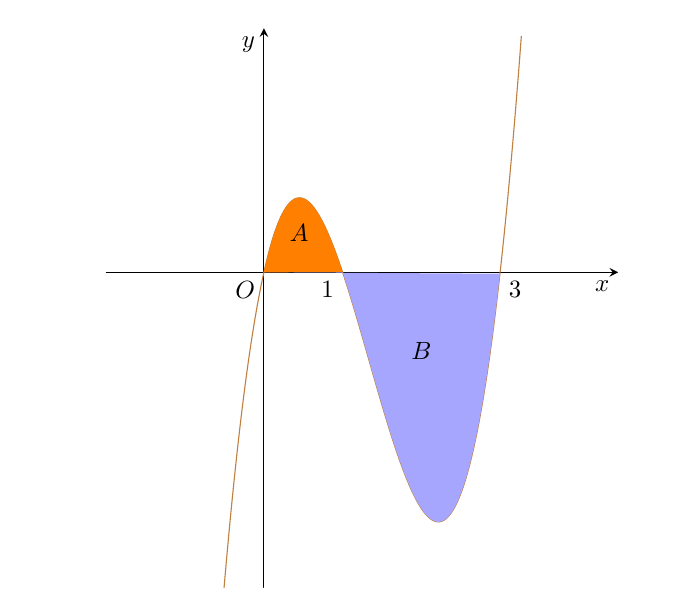
\begin{tikzpicture}[line join=round,line cap=round,>=stealth]
				\tikzset{every  node/.style={scale=0.9}}
				\draw[->] (-2,0)--(4.5,0) node[below left]  {$x$};
				\draw[->] (0,-4)--(0,3.1) node[below left]  {$y$};
				\draw (0,0) node [below left]  {$O$};
				\node at (1,0)  [below left]{$1$};
				\node at (3,0) [below right]{$3$}; 
				\begin{scope}
					\clip (-3,-4) rectangle  (5,3);
					 \draw[brown,samples=200,domain=-1:4,smooth,variable=\x] plot (\x,{1.5*((\x)^3)+-6*((\x)^2)+4.5*(\x)+0});
				\end{scope}
				\fill[orange!100!black!100!] (0,0)--plot[domain=0:1,samples=200] (\x,{1.5*((\x)^3)+-6*((\x)^2)+4.5*(\x)+0})--cycle; 
				\node at (0.45,0.5) {$A$}; 
				\fill[blue!50!white!70!] (0,0)--plot[domain=1:3,samples=200]  (\x,{1.5*((\x)^3)+-6*((\x)^2)+4.5*(\x)+0})--cycle;
				\node at (2,-1) {$B$}; 
			\end{tikzpicture}
	\end{center}
	 \shortans{-4}
	 \loigiai{
		Hình phẳng $A$ được giới hạn bởi đồ thị hàm số $y=f'(x)$, trục hoành $y=0$, trục  tung $x=0$ và đường thẳng $x=1$ nên diện tích hình phẳng $A$ là\\
		\[S_A=\displaystyle\int_0^1 |f'(x)| \mathrm{\,d}x=\displaystyle\int_0^1 f'(x) \mathrm{\,d}x=f(1)-f(0)\] 
		Suy  ra $f(1)=S_A+f(0)=4+2=6$.\\
		Hình phẳng $B$ được giới hạn bởi đồ thị hàm số $y=f'(x)$, trục hoành $y=0$, đường thẳng $x=1$ và đường thẳng $x=3$ nên diện tích hình phẳng $B$ là 
		\[S_B=\displaystyle\int_1^3 |f'(x)|  \mathrm{\,d}x=-\displaystyle\int_1^3 f'(x) \mathrm{\,d}x=-[f(3)-f(1)]=-f(3)+f(1).\]
		Suy  ra $f(3)=f(1)-S_B=6-10=-4$.\\
	Vậy $f  (3)=-4$.}
\end{bt}

% nguồn: Phan2_Lop_12_Dai_so_Chuong_4
\begin{bt}%[2D4V2-6]%[ma:7a0433ac]
	Giả sử lợi nhuận biên (tính theo triệu đồng trên tấn) của một sản phẩm của nhà máy được tính theo công thức $P'(x) = 18-0{,}04x$. Trong  đó $P(x)$ (tính bằng triệu đồng) là lợi nhuận thu được khi bán $x$ tấn sản phẩm. Chênh lệch lợi nhuận khi bán $100$ tấn sản phẩm so với khi bán $50$ tấn sản phẩm là \ldots triệu đồng.
	\shortans{750} 
	\loigiai{ 
		$P=\displaystyle \int_{50}^{100} P'(x) \mathrm{\,d}x = \int_{50}^{100} (18-0{,}04x)  \mathrm{\,d}x = \left(18x-0{,}02x^2\right)\bigg|_{50}^{100} = 750$.\\
		Vậy sự thay đổi  lợi nhuận khi bán được từ $50$ tấn sản phẩm đến $100$ tấn sản phẩm bằng $750$ triệu đồng.
	} 
\end{bt}

% nguồn: Phan2_Lop_12_Dai_so_Chuong_4
\begin{bt}%[2D4V2-6]%[ma:8f23eace]
	\immini{Sân trường có một bồn hoa hình tròn có tâm $O$. Một nhóm học sinh lớp $12$ được giao thiết kế bồn hoa, nhóm này định chia bồn hoa thành bốn  phần, bởi hai đường parabol có cùng đỉnh $O$ và đối xứng nhau qua $O$. Hai đường parabol này cắt đường tròn tại bốn điểm $A$, $B$, $C$, $D$ tạo thành một hình vuông có cạnh bằng $4$ m (như hình vẽ). Phần diện tích $S_1$, $S_2$ dùng để trồng hoa, phần diện tích $S_3$, $S_4$ dùng để trồng cỏ (Diện tích làm tròn đến chữ số thập phân thứ hai). Biết kinh phí để trồng hoa là $150\,000$ đồng/m$^2$, kinh phí để trồng cỏ là $100\,000$ đồng/m$^2$. Để trồng bồn hoa đó nhà trường cần số tiền là bao nhiêu nghìn đồng? (Số tiền làm tròn đến hàng chục nghìn).}
	{\begin{tikzpicture}[>=stealth,x=1cm,y=1cm,scale=1]

		\draw[fill]  (-2,2) circle (1pt) node[above]{$A$}
			(2,2) circle  (1pt) node[above]{$B$}
			(2,-2)  circle (1pt) node[below]{$C$}
			 (-2,-2) circle (1pt) node[below]{$D$}
			(0,1.5)  node[above]{$S_1$}
			(0,-1.5)  node[below]{$S_2$}
			(-1.5,0)  node[left]{$S_3$}
			(1.5,0)  node[right]{$S_4$};
		 \clip (-3.5,-3.5) rectangle (4.5,4.5);
		\draw[samples=150,smooth,domain=-2:2] plot (\x,{0.5*(\x)^2}); 
		 \draw[samples=150,smooth,domain=-2:2] plot (\x,{-0.5*(\x)^2}); \draw[samples=150,smooth,domain=-2.8284:2.8284] plot (\x,{(8-(\x)^2)^0.5});
		\draw[samples=150,smooth,domain=-2.8284:2.8284]  plot (\x,{-(8-(\x)^2)^0.5});
	\end{tikzpicture}}
	 \shortans{3,27}
	 \loigiai{
	\immini{Chọn hệ trục tọa độ như hình vẽ, $O(0;0)$; $A(-2;2)$;  $B(2;2)$.\\
		Khi đó phương trình parabol phía trên có  dạng là
		$(P)\colon y=ax^2$ trong đó $B(2;2)\in (P)\Rightarrow  a=\dfrac{1}{2}$.\\
		Suy  ra $(P)\colon y=\dfrac{x^2}{2}$.\\
		 Phương trình cung tròn nằm phía trên trục $Ox$ là
		 $y=\sqrt{R^2-x^2}=\sqrt{OA^2-x^2}=\sqrt{8-x^2}$.\\
		Khi đó $S_1=\displaystyle\int_{-2}^2\left(\sqrt{8-x^2}-\dfrac{x^2}{2}\right)\mathrm{\,d}x$. (Tính toán $S_1$ là phần khó  của bài này và thường cần kiến thức tích phân).\\
		Diện tích hình tròn là  $S=\pi R^2=\pi OA^2=8\pi$.\\
		Ta có $T=150\cdot 2S_1+100\cdot  (S-2S_1)$ (Tổng chi phí).\\
		Bấm máy ta được $T=150\cdot  2S_1+100\cdot (S-2S_1) \approx 3{,}27$ nghìn đồng. }
		{\begin{tikzpicture}[>=stealth,x=1cm,y=1cm,scale=1]
		\draw[->] (-3.5,0)  -- (4,0) node[below] {$x$};
		\draw[->] (0,-3.5) -- (0,4) node[left]  {$y$};
		 \draw[fill] (0,0) circle (1pt) node[below left]{$O$}
			(-2,2) circle (1pt)  node[above]{$A$}
			(2,2)  circle (1pt) node[above]{$B$}
			(2,-2)  circle (1pt) node[below]{$C$}
			(-2,-2) circle  (1pt) node[below]{$D$}
			 (0,1.5) node[left]{$S_1$}
			(0,-1.5) node[right]{$S_2$} 
			(-1.5,0)  node[below]{$S_3$}
			(1.5,0)  node[above]{$S_4$};
		 \clip (-3.5,-3.5) rectangle (4.5,4.5);
		\draw[samples=150,smooth,domain=-2:2]  plot (\x,{0.5*(\x)^2});
		\draw[samples=150,smooth,domain=-2:2] plot (\x,{-0.5*(\x)^2}); \draw[samples=150,smooth,domain=-2.8284:2.8284] plot  (\x,{(8-(\x)^2)^0.5});
		\draw[samples=150,smooth,domain=-2.8284:2.8284] plot  (\x,{-(8-(\x)^2)^0.5});
	\end{tikzpicture}}
	} 
\end{bt}

% nguồn: Phan2_Lop_12_Dai_so_Chuong_4
\begin{bt}%[2D4V2-6]%[ma:0a324ef5]
	Trong một dịch cúm, tốc độ  tăng số trường hợp mắc bệnh của một thành phố được ước lượng bởi $N'(t)=10 \mathrm{e}^{0{,}2t}$ (trường hợp/ngày) trong đó $N(t)$ là số trường hợp mắc bệnh sau thời gian $t$ ngày kể từ khi bắt đầu dịch. Biết rằng thời điểm bắt đầu dich có $5$ trường hợp mắc bệnh. Ước lượng số trường hợp mắc bệnh của thành phố sau $10$ ngày dịch bắt đầu.
	\shortans{324} 
	 \loigiai{
		Ta có $N(t)= \displaystyle\int N'(t)\mathrm{\,d}t = \displaystyle\int  10\mathrm{e}^{0{,}2t}\mathrm{\,d}t = 10 \dfrac{\mathrm{e}^{0{,}2t}}{\ln\mathrm{e}^{0{,}2}}+C=50 \mathrm{e}^{0{,}2t}+C$.\\
		Theo giả thiết $N(0)=5 \Rightarrow 50+C=5  \Rightarrow C=-45$.\\
		Vậy $N(t)=50 \mathrm{e}^{0{,}2  t}-45$.\\
		$N(10)=50 \mathrm{e}^{0{,}2\cdot 10}-45  \approx 324$ (trường hợp).
	} 
\end{bt}

% nguồn: Phan2_Lop_12_Dai_so_Chuong_4
\begin{bt}%[2D4V2-6]%[ma:f639940f]
	Một vật chuyển động thẳng. Khi vật bắt đầu qua điểm $O$, người ta bắt đầu quan sát, đo đạc chuyển động của vật thì thấy vận tốc tức thời của vật tại thời điểm $t(s)$ là $v(t)$ (m/s), hàm vận tốc $v(t)$ có đồ thị phụ thuộc thời gian là một phần của đường parabol đỉnh $I\left(\dfrac{4}{3};-\dfrac{7}{3}\right)$ như hình bên (với $t\ge 0$ và mốc tính thời gian là lúc bắt đầu quan sát chuyển động). Tính tổng quãng đường vật đi được từ lúc đầu  đến lúc vật trở lại điểm $O$ lần cuối cùng (kết quả tính bằng mét và làm tròn đến hàng phần trăm).
	\begin{center}
		\begin{tikzpicture}[scale=0.9,font=\footnotesize,line join=round,line cap=round,>=stealth];
				\draw[->] (-1,0) -- (4,0)  node[below] {\scriptsize $t$};
				\draw[->] (0,-3)  -- (0,4) node[left] {\scriptsize $v$};
				\draw (0.1,0.1)  node[below left]{\scriptsize $O$};
				 \draw[thin,samples=150,smooth,domain=0:2.7] plot (\x,{3.0*((\x)^2)-8*(\x)+3});
				\draw[dashed] (4/3,0) node[above]{$\dfrac{4}{3}$}--(4/3,-7/3)  node[below]{$I$}--(0,-7/3) node[left]{$-\dfrac{7}{3}$}
					(0,3)  node[left]{$3$};
				\draw (0,3) circle  (1.2pt)
					(4/3,-7/3) circle (1.2pt); 
			\end{tikzpicture}
	\end{center}
	\shortans{5,49} 
	 \loigiai{
		 Gọi $v(t)=at^2+bt+c$.
		Dựa vào đồ thị ta  thấy\\
		$$\heva{&c=3\\&\dfrac{-b}{2a}=\dfrac{4}{3}\\&a\cdot \left(\dfrac{4}{3}\right)^2+b\cdot \dfrac{4}{3}+c=-\dfrac{7}{3}}\Rightarrow \heva{&a=3\\&b=-8\\&c=3} \Rightarrow  v(t)=3t^2-8t+3\,(\text{m/s}).$$
		 Khi đó $\displaystyle\int v(t)\,\mathrm{\,d}t=t^3-4t^2+3t+C\Rightarrow s(t)=t^3-4t^2+3t+C$.\\
		 Vì $s(0)=0\Rightarrow s(t)=t^3-4t^2+3t$.\\
		Tại các thời điểm vật qua  $O$ ứng với $t$ thoả mãn $s(t)=0\Leftrightarrow \hoac{&t=0\\ &t=3.}$\\
		Do đó thời điểm cuối vật qua $O$ là $t=3(s)$ nên tổng quảng đường vật đi được từ lúc đầu đến lúc vật trở lại  điểm $O$ lần cuối cùng là
		 $$S=\displaystyle\int^3_0|v(t)|\mathrm{\,d}t=\displaystyle\int^3_0\left|3t^2-8t+3\right|\mathrm{\,d}t\approx 5{,}49\,(\text{m}).$$
	} 
\end{bt}

% nguồn: Phan2_Lop_12_Dai_so_Chuong_4
\begin{bt}%[2D4C2-6]%[ma:4cf43bc8]
	Giả sử anh Nam nhảy dù từ một chiếc trực thăng. Vào thời  điểm $19$ giây sau khi rời khỏi trực thăng, anh Nam mở chiếc dù của mình trong $2$ giây, anh Nam chạm đất sau $19$ giây kể từ lúc bung dù. Tại thời điểm $t$ (giây), vị trí của anh Nam cách mặt đất một khoảng $h(t)$ mét và vận tốc rời của anh Nam (tính bằng m/s) là một hàm số được cho bởi công thức: $$v(t)=h'(t)=\heva{&-80&\text{ khi }& 0 \le t < 19\\&37t-783&\text{ khi }& 19 \le t < 21\\&-6&\text{ khi }& 21 \le t \le 40.}$$
	Độ cao vị trí của anh Nam khi bắt  đầu nhảy ra khỏi trực thăng bằng \ldots m.
	 \shortans{1,72}
	 \loigiai{
	\begin{flalign*}
		h&=\displaystyle \int_{0}^{40} \left|h'(t)\right| \mathrm{\,d}t = \int_{0}^{19} \left|-80\right| \mathrm{\,d}t + \int_{19}^{21} \left|37t-783\right| \mathrm{\,d}t  + \int_{21}^{40} \left|-6\right| \mathrm{\,d}t&\\
		&=80t\bigg|_{0}^{19} + \left(783t-\dfrac{37t^2}{2}\right)\bigg|_{19}^{21} + 6t\bigg|_{21}^{40} =  1\,720.
	\end{flalign*}
	 }
\end{bt}

% nguồn: Phan2_Lop_12_Dai_so_Chuong_4
\begin{bt}%[2D4C2-6]%[ma:9ab51bc6]
	Tại một địa điểm, trong khoảng thời gian $12$ giờ nhiệt độ tại thời điểm $t$ (tính bằng giờ kể từ lúc bắt đầu) là $T(t)=47+4t-\dfrac{1}{3}t^2\ \left({}^{\circ}\text{ C}\right)$. Nhiệt độ trung bình trong khoảng thời gian  đó bằng \ldots ${}^{\circ}$C.
	 \shortans{55}
	 \loigiai{
	$\overline{T} = \dfrac{1}{12-0}\displaystyle \int_{0}^{12} T(t) \mathrm{\,d}t = \dfrac{1}{12}\int_{0}^{12} \left(47+4t-\dfrac{1}{3}t^2\right)  \mathrm{\,d}t = \left(47t+2t^2-\dfrac{1}{9}t^3\right)\bigg|_{0}^{12}=55$.
	} 
\end{bt}


%%%%%%%%%%%%%%%% TỰ LUẬN %%%%%%%%%%%%%%%%

% nguồn: Phan2_Lop_12_Dai_so_Chuong_4
\begin{bt}%[2D4H2-6]%[ma:04f9d921]
	Biết rằng tốc độ $v$ (km/phút) của một ca-nô cao tốc thay đổi theo thời  gian $t$ (phút) như sau
	\[v(t)=\heva{&0{,}5t&&\text{ với}\,0\leq t <  2\\
	 &1{,}2 &&\text{ với}\,2\leq t < 15\\
	&4-0{,}2t&&\text{  với}\,15\leq t\leq 20.}\]
	Tính quang đường ca-nô di chuyển được trong khoảng thời gian  từ $0$ tới $20$ phút.
	 \loigiai{
		Quãng đường chuyển  động của ca-nô là
		 \allowdisplaybreaks
		\begin{eqnarray*}
			S&=&\int_0^{20}v(t)\mathrm{\,d}t\\ 
			&=&\int_0^2(0,5t)\mathrm{\,d}t+\int_2^{15}1\mathrm{~d}t+\int_{15}^{20}(4-0,2t)\mathrm{\,  d}t\\
			 &=&\dfrac{t^2}{4}\bigg|_0^2+t\bigg|_2^{15}+\left(4t-\dfrac{1}{10}t^2\right)\bigg|_{15}^{20}\\
			 &=&1+15-2+40-37{,}5\\
			 &=&16{,}5\ (\mathrm{km}).
		\end{eqnarray*}
	} 
\end{bt}

% nguồn: Phan2_Lop_12_Dai_so_Chuong_4
\begin{bt}%[2D4H2-6]%[ma:f639aef3]
	Cô Hạnh đổ bê tông một đường đi trong vườn (phần được tô màu) với kích thước được cho trong hình sau. Biết rằng đường cong $AB$ được cho bởi đồ thị của một hàm số liên tục và đường cong $DC$ nhận được từ đường cong $AB$ bằng cách tịnh tiến theo phương thẳng đứng lên phía trên $2$ m. Ngoài ra, cô Hạnh quyết định đổ lớp bê tông dày $15$  cm và giá tiền $1$ m$^3$ bê tông là $1\, 080\, 000$ đồng. Tính số tiền cô Hạnh cần dùng để đổ bê tông con đường đó.
	\begin{center}
		\begin{tikzpicture}[declare function={r=3; d=5; a=1;},>=latex]
				\fill[gray!45] (0,r) coordinate (D) to [out=0,in=180] (d,a) coordinate (C) 
					--  (d,0) coordinate (B) to [out=180,in=0] (0,{r-a}) coordinate (A)--cycle;
				\draw (0,r)  to [out=0,in=180] (d,a)
					(0,{r-a}) to  [out=0,in=180] (d,0);
				\draw  (0,0) rectangle (d,r);
				\foreach \t/\g in {D/180,C/0,B/0,A/180}{ 
					\path (\t) circle  (1pt) node[shift={(\g:9pt)},font=\scriptsize]{$\t$};
				} 
				\draw[<->] ($(B)+(19pt,0)$) --  ($(C)+(19pt,0)$) node[pos=0.5,right]{$2$ m};
				\draw[<->] ($(D)-(19pt,0)$)  -- (-19pt,0) node[pos=0.5,left]{$6$ m};
				\draw[<->] ($(B)-(0,9pt)$) -- (0,-9pt) node[pos=0.5,below]{$10$ m}; 
			\end{tikzpicture}
	\end{center}
	\loigiai{ 
		Để tính diện tích phần  đổ bê tông, ta cần xác định diện tích giữa hai đường cong $AB$ và $DC$.\\
		Đường cong $DC$  là kết quả của việc tịnh tiến đường cong $AB$ lên trên $2$ m.\\
		Giả sử hàm số của đường cong $AB$ là $f(x)$  thì hàm số của đường cong $DC$ là $f(x)+2$.\\
		Diện tích hình phẳng giới hạn bởi  hai đường cong là: $S=\displaystyle\int_0^{10}\left[f(x)+2-f(x)\right] \mathrm{d}x=20\mathrm{~m}^2$.\\
		Lớp bê tông  có độ dày là $15$ cm tức là $0{,}15$ m thì có thể tích là: $20\cdot 0{,}15=3\mathrm{~m}^3$.\\
		Chi phí tổng  cộng để đổ bê tông con đường đó là: $3\cdot 1\,080\,000=3\,240\,000$ (đồng)$=3240$ (triệu đồng).
	} 
\end{bt}

% nguồn: Phan2_Lop_12_Dai_so_Chuong_4
\begin{bt}%[2D4H2-6]%[ma:adf1faa3]
	Giả sử rằng sau $t$ năm, vốn đầu tư của một doanh nghiệp phát sinh lợi nhuận với tốc độ $P'(t)=126+t^2$ (triệu đồng/năm). Hỏi sau $10$ năm đầu tiên thì doanh nghiệp thu được lợi nhuận là bao nhiêu (đơn  vị triệu đồng)?
	\loigiai{ 
		Gọi $P(t)$ là lợi nhuận phát sinh của vốn sau $t$  năm đầu tư. Ta có $P(t)$ là nguyên hàm của hàm tốc độ $P'(t)$.\\
		Lợi nhuận phát sinh sau $10$ năm đầu  tiên là
		$$\displaystyle \int_0^{10}P'(t)\mathrm{\,d}t=\int_0^{10}(126+t^2)\mathrm{\,d}t=\dfrac{4780}{3}\text{ (triệu đồng).}$$ 
	 }
\end{bt}

% nguồn: Phan2_Lop_12_Dai_so_Chuong_4
\begin{bt}%[2D4H2-6]%[ma:18374b8a]
	Khảo sát chuyển động của xe khách $A$ trong $30$ phút trên một quãng đường ta thu được kết quả: vận tốc $v$ (m/phút) của  xe khách theo thời gian $t$ (phút) được biểu diễn bởi hàm số
	$$ 
	v(t)=\heva{& 100t,&&0\leq t\leq  10\\&20t+800,&&10<t\leq 20\\&-10t+1400,&&20<t\leq 30.}
	 $$
	Tính quãng đường chuyển động và vận tốc  trung bình của xe khách trong $30$ phút đã khảo sát.
	\loigiai{Quãng đường chuyển động của xe khách trong $30$ phút khảo sát là \allowdisplaybreaks\begin{eqnarray*}
		 S&=&\int_0^{30}v(t)\mathrm{\,d}t\\
		&=&\int_0^{10}v(t)\mathrm{\,d}t+\int_{10}^{20}v(t)\mathrm{\,d}t+\int_{20}^{30}v(t)\mathrm{\,d}t\\ 
		&=&\int_0^{10}100t\mathrm{\,d}t+\int_{10}^{20}(20t+800)\mathrm{\,d}t+\int_{20}^{30}(-10t+1400)\mathrm{\,d}t\\ 
		&=&27\,500\  (\mathrm{m}).
	\end{eqnarray*}
 Vận tốc trung bình của xe khách trong $30$ phút khảo sát là $$v_\text{ tb}=\dfrac{S}{30}=\dfrac{2\,750}{3}\approx 917\ (\text{m/phút}).$$}
\end{bt}

% nguồn: Phan2_Lop_12_Dai_so_Chuong_4
\begin{bt}%[2D4H2-6]%[ma:ea824c6f]
	Một vật chuyển động với vận tốc $v(t)=3-\sin t$ (m/s). Tính quãng đường vật đi chuyển trong khoảng thời gian  từ thời điểm $t=0$ đến thời điểm $t=\dfrac{\pi}{2}$.
	\loigiai{ 
		Ta có  quãng đường vật đi chuyển trong khoảng thời gian từ thời điểm $t=0$ đến thời điểm $t=\dfrac{\pi}{2}$ là
		\[ 
		S=\displaystyle\int_0^{\tfrac{\pi}{2}}v(t)\mathrm{\,d}t=\displaystyle\int_0^{\tfrac{\pi}{2}}(3-\sin  t)\mathrm{\,d}t=\left(3t+\cos t\right)\Big|_0^{\tfrac{\pi}{2}}=\left(3\cdot\dfrac{\pi}{2}+\cos\dfrac{\pi}{2}\right)-(3\cdot0+\cos0)=\dfrac{3\pi}{2}-1.
		 \]
		Vậy quãng đường vật di chuyển trong khoảng thời gian từ thời điểm $t=0$ đến  thời điểm $t=\dfrac{\pi}{2}$ là $\dfrac{3\pi}{2}-1$ mét.
	 }
\end{bt}

% nguồn: Phan2_Lop_12_Dai_so_Chuong_4
\begin{bt}%[2D4H2-6]%[ma:eb820ff8]
	Giả sử tốc độ $v$ (m/s) của một thang máy di chuyển từ tầng $1$ lên tầng cao nhất theo thời gian $t$ (giây) được cho  bởi công thức: $$v(t)=\heva{&t,&&0\leq t\leq 2\\&2,&&2<t\leq 20\\&12-0{,}5t,&&20<t\leq 24.}$$
	Tính quãng đường chuyển động và tốc độ trung bình của thang  máy.
	\loigiai{ 
		Gọi $s(t)$ là quãng đường thang máy di chuyển được đến thời  gian $t$ (giây).\\
		Quãng đường thang máy di chuyển từ tầng $1$ lên tầng cao  nhất là
		\allowdisplaybreaks\begin{eqnarray*}
		s&=&s(20)-s(0)=\int_0^{20}v(t)\mathrm{\,d}t\\ 
		&=&\int_0^2v(t)\mathrm{\,d}t+\int_2^{20}v(t)\mathrm{\,d}t+\int_{20}^{24}v(t)\mathrm{\,d}t=\int_0^2t\mathrm{~d}t+\int_2^{20}2\mathrm{~d}t+\int_{20}^{24}(12-0{,}5t)\mathrm{\,d}t\\ 
		&=&\left(\dfrac{t^2}{2}\right)\bigg|_0^2+(2t)\bigg|_2^{20}+\left(12t-\dfrac{0{,}5t^2}{2}\right)\bigg|_{20}^{24}=42\  (\mathrm{m}).
	\end{eqnarray*}
	Vận tốc trung bình của thang máy là  $v_\text{ tb}=\dfrac{s}{t}=\dfrac{42}{24}=1{,}75$ (m/s).
} 
\end{bt}

% nguồn: Phan2_Lop_12_Dai_so_Chuong_4
\begin{bt}%[2D4H2-6]%[ma:0931664a]
	Tốc độ $v$ (m/s) của một thang máy di chuyển từ tầng $1$ lên tầng cao nhất theo thời gian $t$ (giây) được cho bởi công thức 
	\[v(t)=\heva{&t&&\text{  với}\,0\leq t\leq 2\\
	 &2&&\text{ với}\,2<t\leq 20\\
	 &12-0{,}5t&&\text{ với}\,20<t\leq 24.}\]
	Tính quãng đường chuyển động và  tốc độ trung bình của thang máy.
	\loigiai{ 
		Quãng đường chuyển động của  thang máy là
		\allowdisplaybreaks\begin{eqnarray*}
		S&=&\int_0^{24}v(t)\mathrm{\,d}t\\ 
		&=&\int_0^2t\mathrm{~d}t+\int_2^{20}2\mathrm{~d}t+\int_{20}^{24}(12-0{,}5t)\mathrm{\,d}t\\ 
		&=&\dfrac{t^2}{2}\bigg|_0^2+2t\bigg|_2^{20}+\left(12t-\dfrac{1}{4}t^2\right)\bigg|_{20}^{24}\\ 
		&=&2+40-4+144-140\\ 
		&=&42\,(\mathrm{m}). 
	\end{eqnarray*}
	 Tốc độ trung bình của thang máy là $v_{tb}=\dfrac{S}{t}=\dfrac{42}{24}=1{,}75$\,(m/s).
 }
\end{bt}

% nguồn: Phan2_Lop_12_Dai_so_Chuong_4
\begin{bt}%[2D4H2-6]%[ma:6a6d8b26]
	Một vật chuyển động dọc theo một đường thẳng sao cho vận tốc của nó  tại thời điểm $t$ (giây) là $v(t)=t^2-t-6$ (m/s).
	\begin{enumerate}
		\item Tìm độ dịch chuyển của vật trong  khoảng thời gian $1\leq t \leq 4$, tức là tính $\displaystyle\int_1^4v(t) \mathrm{\,d
		 }t$.
		\item Tìm tổng quãng đường  vật đi được trong khoảng thời gian này, tức là tính $\displaystyle\int_1^4|v(t)|\mathrm{\,d
		 }t$.
	\end{enumerate}
	\loigiai{ 
		\begin{enumerate}
			\item Độ dịch chuyển của vật trong khoảng thời gian $1\leq t \leq 4$ là \begin{eqnarray*}
			\int_1^4 v(t) \mathrm{\,d}t&=&\int_1^4\left(t^2-t-6\right) \mathrm{\,d}t\\ 
			&=&\left.\left(\dfrac{t^3}{3}-\dfrac{t^2}{2}-6 t\right)\right|_1^4\\ 
			 &=&\left(\dfrac{4^3}{3}-\dfrac{4^2}{2}-6 \cdot 4\right)-\left(\dfrac{1}{3}-\dfrac{1}{2}-6\right)\\
			&=&-\dfrac{9}{2}. 
		\end{eqnarray*}
		\item Tổng quãng đường vật đi được trong khoảng thời gian $1\leq t \leq 4$ là \begin{eqnarray*}
		 \int_1^4|v(t)|\mathrm{\,d}t&=&\int_1^4\left|t^2-t-6\right|\mathrm{\,d}t\\
		&=&\int_1^3\left(-t^2+t+6\right)  \mathrm{\,d}t+\int_3^4\left(t^2-t-6\right) \mathrm{\,d}t\\
		 &=&\dfrac{22}{3}+\dfrac{17}{6}\\
		 &=&\dfrac{61}{6}.
	\end{eqnarray*}
	\end{enumerate}
 }
\end{bt}

% nguồn: Phan2_Lop_12_Dai_so_Chuong_4
\begin{bt}%[2D4H2-6]%[ma:18b2835f]
	Xét chiếc chén trong một bộ ấm chén uống trà, bạn Dương ước lượng được  rằng chiếc chén được tạo thành khi cho hình phẳng giới hạn bởi đồ thị hàm số $f(x)=0{,}14x^3-0{,}87x^2+1{,}92x+0{,}85$, trục hoành và hai đường thẳng $x=0$, $x=3$ quay quanh trục $Ox$ (đơn vị trên mỗi trục toạ độ là centimét). Tính thể tích của chiếc chén (làm tròn đến hàng đơn vị của centimét khối).
	\begin{center}
		\resizebox{!}{5cm}{\begin{tikzpicture}[line cap=butt,line join=miter,>=stealth]
		\draw[->]  (-1,0)--(0,0)
			(3,0)--(4.5,0) 
			node[shift={(-100:7pt)},font=\normalsize]{$x$}; 
		 \draw[->] (0,-3)--(0,3.5)
			node[shift={(180:7pt)},font=\normalsize]{$y$}; 
		\draw[dashed] (0,0)--(3,0); 
		\draw (5pt,0) |-  (0,5pt)
			(0,0) node[shift={(225:9pt)},font=\normalsize]{$O$}; 
		\foreach \x in {-1,1,2,3}{ 
			 \draw (\x,1.5pt)--(\x,-1.5pt) node[font=\scriptsize,shift={(-90:5pt)}]{\x};
		} 
		\foreach \y in  {-2,-1,1,2,3}{
			 \draw (1.5pt,\y)--(-1.5pt,\y) node[font=\scriptsize,shift={(180:5pt)}]{\y};
		 }
		\tikzset{declare function={f  (\x)=(14/100)*(\x)^3-(87/100)*(\x)^2+(192/100)*(\x)+85/100; a=f (3);}}
		 \draw[samples=100] plot[domain=0:3] (\x,{f (\x)});
		\draw[samples=100] plot[domain=0:3] (\x,{-f  (\x)});
		\draw (3.05,0) ellipse ({0.25*a} and  a);
		 \path (1.5,{f (1.5)}) node[above]{$y=f (x)$};
	\end{tikzpicture}}
	\end{center}
	\loigiai{ 
		Thể tích của chiếc chén  là: $V=\pi\displaystyle\int_0^3\left(0{,}14x^3-0{,}87x^2+1{,}92x+0{,}85\right)^2\mathrm{d}x=41{,}87\,(\mathrm{cm}^3)$.
	 }
\end{bt}

% nguồn: Phan2_Lop_12_Dai_so_Chuong_4
\begin{bt}%[2D4V2-6]%[ma:0a9fae6b]
	Việc thở là những vòng tuần hoàn, mỗi vòng tính từ lúc bắt đầu hít vào đến lúc kết thúc thở ra, thường kéo dài trong $5$s. Vận tốc cực đại của khí là $V$  (l/s) nên vì thế nó được mô hình hoá bởi công thức $v(t)=V\sin \dfrac{3\pi t}{5}$. Tính thể tích khí hít vào phổi sau thời gian $2$s.
	\loigiai{ 
		Vận tốc của khí hít vào được mô hình bởi công thức $v(t)=V\sin \dfrac{3\pi t}{5}$.\\ 
		Suy ra lượng  khí hít vào sau $2$ giây là
		 $$\displaystyle N(2)=\int_0^2v(t)\mathrm{\,d}t
		=\int_0^2V\sin  \dfrac{3\pi t}{5}\mathrm{\,d}t
		=\dfrac{5V}{3\pi}\left(1-\cos \dfrac{3\pi\cdot 2}{5}\right)=0{,}06V\text{  (lít).}$$
	} 
\end{bt}

% nguồn: Phan2_Lop_12_Dai_so_Chuong_4
\begin{bt}%[2D4V2-6]%[ma:a59a4832]
	 Một người đang lái ô tô với vận tốc $72$ km/h thì gặp chướng ngại vật, người đó đạp phanh và ô tô bắt đầu chuyển động chậm dần đều với vận tốc cho bởi phương trình $v(t) = a + bt$ m/s, trong đó $a$ và $b$ là các hằng số và $t\geq 0$ là khoảng thời gian tính từ lúc người đó bắt đầu đạp phanh. Biết quãng đường ô tô đi được từ lúc đạp phanh cho đến lúc dừng lại là $40$ m. Tính thời gian ô tô chuyển động từ lúc người đó đạp phanh đến khi ô tô dừng hẳn.
	 \loigiai{
		Đổi $72$ km/h $=  20$ m/s.\\
		Vì người đó đạp phanh  khi đang chuyển động với vận tốc $20$ m/s nên $a=20$.\\
		Ô tô dừng hẳn khi $v(t) = 0 \Leftrightarrow a + bt = 0 \Leftrightarrow t = -\dfrac{a}{b}  = -\dfrac{20}{b}$.\\
		Quãng đường ô tô đi được từ lúc đạp phanh đến khi dừng hẳn  là
		\[ 
		S=\displaystyle\int_0^{-\tfrac{20}{b}} v(t)\mathrm{\,d}t=\displaystyle\int_0^{-\tfrac{20}{b}} (20 + bt)\mathrm{\,d}t = \left(20t + \dfrac{bt^2}{2}\right)\Bigg|_0^{-\tfrac{20}{b}} = -\dfrac{400}{b} + \dfrac{200}{b}  = -\dfrac{200}{b}.
		\] 
		Vì ô tô đi được quãng đường là $40$ m nên $-\dfrac{200}{b} = 40 \Rightarrow b  = -5$.\\
		Do đó thời gian ô tô chuyển động từ lúc người đó đạp phanh  đến khi ô tô dừng hẳn là
		 \[
		\dfrac{-20}{-5} = 4. 
		\] 
		Vậy ô  tô dừng hẳn sau $4$ giây.
	} 
\end{bt}

% nguồn: Phan2_Lop_12_Dai_so_Chuong_4
\begin{bt}%[2D4V2-6]%[ma:fd1aadae]
	Để đảm bảo an toàn khi lưu thông trong thành phố thì các  xe khi dừng lại phải cách nhau một khoảng tối thiểu là $1$ m. Một xe máy di chuyển trên đường thì gặp đèn đỏ từ xa, người điều khiển xe máy đạp phanh và xe chuyển động chậm dần đều với vận tốc $v(t)=10-5t$ (m/s). Hỏi để giữ khoảng cách an toàn, người điều khiển xe máy phải bắt đầu đạp phanh khi cách xe đang dừng phía trước tối thiểu một khoảng bao xa, biết rằng ngay lúc đạp phanh thì xe phía trước đang đứng yên?
	\loigiai{ 
		Kể từ lúc đạp phanh $(t = 0)$ đến  lúc xe dừng lại thì xe đi được một quãng đường là $s$. \\
		Vì khoảng cách an toàn giữa $2$ xe khi dừng lại tối thiểu là $1$m nên người điều khiển xe máy phải bắt đầu đạp phanh khi cách xe đang dừng phía trước tối thiểu một  khoảng $s + 1$ (m).\\
		Tại thời điểm  $t=0$ thì xe bắt đầu phanh, và xe dừng lại khi vận tốc bằng $0$, khi đó:
		$$v(t)=0\Leftrightarrow  10-5t=0\Leftrightarrow t=2.$$
		Trong khoảng thời gian từ $t=0$ s đến $t=2$ s thì xe chạy thêm được  quãng đường
		$$\displaystyle s=\int_0^2(10-5t)\mathrm{\,d}t=10\,  \mathrm{(m).}$$
		Vậy xe nên bắt đầu đạp phanh khi cách xe đang dừng phía trước tối  thiểu một khoảng $11$m để giữ khoảng cách an toàn.
	} 
\end{bt}

% nguồn: Phan2_Lop_12_Dai_so_Chuong_4
\begin{bt}%[2D4V2-6]%[ma:0651f0f3]
	Một vật chuyển động với  vận tốc được cho bởi đồ thị ở hình vẽ:
	\begin{center}
		\begin{tikzpicture}
				 \def\xmax{8.7}
				\def\ymax{4.7} 
				\draw[->] (0,-.5) -- (0,\ymax) node[above left]{$v \text{ (m/s)}$}; 
				\draw[->]  (-.5,0) -- (\xmax,0) node[above right] {$t \text{ (s)}$};
				\node at (0,0) [below left]  {O};
				 \draw (0,0)--(3,4)--(4.5,2)--(8,2);
				\draw[dashed] (0,4) node[left]{$4$}--(3,4)--(3,0)  node[below]{$3$}
					 (0,2) node[left]{$2$}--(4.5,2)--(4.5,0) node[below]{$4{,}5$}
					(8,2)--(8,0)  node[below]{$8$};
			\end{tikzpicture}
	\end{center}
	\begin{enumerate}
		\item Tính quãng đường mà vật di  chuyển được trong $3$ giây đầu tiên.
		\item Tính quãng đường và vật di chuyển  được trong $8$ giây đầu tiên.
	\end{enumerate}
	\loigiai{ 
		\begin{enumerate}
			 \item Dựa vào đồ thị trong khoảng thời gian $3$ giây vận tốc của chuyển động được xác định là $v(t)=\dfrac{4}{3}t$ (m/s). \\
			Ta có quãng  đường mà vật di chuyển được trong $3$ giây đầu tiên là
			 $$\displaystyle s=\int_0^3\dfrac{4}{3}t\mathrm{\,d}t=\dfrac{2}{3}t^2\bigg|_0^3=6\text{ (m).}$$
			\item Dựa vào đồ thị ta thấy trong khoảng thời gian $1$ giây vận tốc của chuyển động được xác định là $v(t)=\dfrac{4}{3}t$ (m/s), khoảng thời gian từ $3$ giây đến $4{,}5$ giây vận tốc của chuyển động được xác định là $v(t)=\dfrac{-4}{3}t+8$ (m/s), khoảng thời gian từ $4{,}5$  giây đến $8$ giây vận tốc của chuyển động là $v(t)=2$ (m/s). \\
			Ta có quãng đường mà vật di chuyển được trong $8$  giây đầu tiên là
			$$\displaystyle s=\int_0^3\dfrac{4}{3}t\mathrm{\,d}t+\int_3^{4,5}\left(-\dfrac{4}{3}t+8\right)\mathrm{\,d}t+\int_{4,5}^8  2\mathrm{\,d}t=17,5\text{ (m).}$$
		\end{enumerate}
	 }
\end{bt}

% nguồn: Phan2_Lop_12_Dai_so_Chuong_4
\begin{bt}%[2D4V2-6]%[ma:b1cacfba]
	 Một chất điểm chuyển động theo quy luật vận tốc $v(t)$\,(m/s) có dạng đường parabol khi $0\leq t\leq 5$\,(s) và $v(t)$ có dạng đường thẳng khi $5\leq t\leq 10$ (s) (xem hình vẽ bên dưới). Biết đỉnh parabol là $I(2,3)$. Hỏi quãng đường đi được chất điểm trong thời gian $0\leq t\leq 10$\,(s) là bao nhiêu mét?
	\begin{center}
		\begin{tikzpicture}[scale=1,font=\footnotesize,line join=round,line cap=round,>=stealth,x=0.3cm,y=0.3cm,declare function = {f (\x) =2*(\x)^2-8*(\x)+11; g (\x)=-21*(\x)/5+42;}]
				 \def \xmin{-2.0};
				\def  \xmax{12.7};
				\def \ymin{-1.5}; 
				 \def \ymax{24.5};
				\draw[->] (\xmin,0.) -- (\xmax,0.) node[anchor=north] {$x$}; 
				\draw[->] (0.,\ymin)  -- (0.,\ymax) node[anchor=west] {$y$};
				 \clip (\xmin+0.1,\ymin+0.1) rectangle (\xmax-0.1,\ymax-0.1);
				\draw[smooth,samples=100,domain=0:5]  plot (\x,{f (\x)});
				 \draw[smooth,samples=100,domain=5:10] plot (\x,{g (\x)});
				\draw[dashed] (2,0) node[below]{$2$} |-  (0,3) node[left]{$3$}
					(5,0) node[below]{$5$} |- (0,21)  node[left]{$21$};
				\foreach \x/\y/\l/\g in {0/0/O/225,2/0//0,5/0//0,10/0/10/-90,2/3//0,5/21//0,0/11/11/180,0/21//0}{\fill (\x,\y)  circle (1pt)+(\g:1) node{$\l$};}
			\end{tikzpicture}
	\end{center}
	\loigiai{ 
		Gọi parabol $(P)\colon y=at^2+bt+c$ là phương trình thể hiện vận tốc của chất  điểm khi $0\leq t\leq 5$\,(s).\\
		Do $(P)$  có đỉnh $I(2;3)$ và đi qua $A(0;11)$ nên
		 $$\heva{&\dfrac{-b}{2a}=2\\&y(0)=11\\&y(2)=3}\Leftrightarrow \heva{&4a+b=0\\&c=11\\&4a+2b+c=3}\Leftrightarrow\heva{&a=2\\&b=-8\\&c=11.}$$
		Suy ra $(P)\colon y=2t^2-8t+11$.\\ 
		Gọi $d\colon y=at+b$ là phương trình đường thẳng thể hiện  vận tốc của chất điểm khi $5\leq t\leq 10$ (s).\\
		Vì $d$ đi qua điểm $B(5;11)$ và $C(10;0)$  nên
		$$\heva{&5a+b=11\\ 
		 &10a+b=0}\Rightarrow \heva{&a=-\dfrac{21}{5}\\
		&b=42}\Rightarrow  y=\dfrac{-21}{5}t+42.$$
		Như vậy phương  trình biểu thị vận tốc của chất điểm là $$v(t)=\heva{&2t^2-8t+11&&0\leq t\leq 5\\&\dfrac{-21}{5}t+42,&&5< t\leq 10.}$$\\
		Khi đó  quãng đường vật di chuyển trong khoảng thời gian từ $0\leq t\leq 10$ (s) là
		\allowdisplaybreaks\begin{eqnarray*}
		S&=&\int_0^{10}v(t)\mathrm{\,d}t\\ 
		 &=&\int_0^5\left(2t^2-8t+11\right)\mathrm{\,d}t+\int_5^{10}\left(\dfrac{-21}{5}t+42\right)\mathrm{\,d}t\\
		 &=&\left(\dfrac{2t^3}{3}-4t^2+11t\right)\bigg|_0^5+\left(\dfrac{-21t^2}{10}+42t\right)\bigg|_5^{10}\\
		&=&\dfrac{115}{3}+\dfrac{105}{2}\\ 
		&=&\dfrac{545}{6}\  (\mathrm{m}).
	\end{eqnarray*}
} 
\end{bt}

% nguồn: Phan2_Lop_12_Dai_so_Chuong_4
\begin{bt}%[2D4V2-6]%[ma:2707aad0]
	Cho hình vẽ dưới  đây là đồ thị vận tốc $v(t)$ của một vật ($t=0$ là thời điểm vật bắt đầu chuyển động).
	\begin{center}
		\begin{tikzpicture}[scale=1,font=\footnotesize,line join=round,line cap=round,>=stealth,x=0.6cm,y=0.6cm]
				 \def \xmin{-1.5};
				\def \xmax{12.6}; 
				\def  \ymin{-1.5};
				 \def \ymax{5.5};
				\draw[->,line width=1pt] (\xmin,0.) -- (\xmax,0.) node[anchor=north] {$x$}; 
				\draw[->,line width=1pt] (0.,\ymin) -- (0.,\ymax) node[anchor=west]  {$y$};
				 \clip (\xmin+0.1,\ymin+0.1) rectangle (\xmax-0.1,\ymax-0.1);
				 \draw[line width=1pt] (0,0)--(2,1) node[above]{$B$}--(4,3) node[above]{$C$}--(7,3) node[above]{$D$}--(10,1) node[right]{$E$};
				\foreach \x/\y/\l/\g in {0/0/O/225}{\fill  (\x,\y) circle (1pt)+(\g:0.5) node{$\l$};}
			\end{tikzpicture}
	\end{center}
	Tính quãng  đường chuyển động và vận tốc trung bình của vật $10$ giây đầu tiên.
	 \loigiai{
		 Phương trình đường thẳng $OB\colon v=\dfrac{1}{2}t$.\\
		Phương trình đường thẳng $BC\colon v=t-1$.\\ 
		Phương  trình đường thẳng $CD\colon v=3$.\\
		Phương trình đường thẳng  $DE\colon v=-\dfrac{2}{3}t+\dfrac{23}{3}$.\\
		Suy ra  $$v(t)=\heva{&\dfrac{1}{2}t,&&0\leq t\leq 2\\&t-1,&&2<t\leq 4\\&3,&&4<t\leq 7\\&-\dfrac{2}{3}t+\dfrac{23}{3},&&7<t\leq 10.}$$
		Quãng  đường chuyển động của vật trong $10$ giây là
		\allowdisplaybreaks\begin{eqnarray*}
		 S&=&\int_0^{10}v(t)\mathrm{\,d}t=\int_0^2v(t)\mathrm{\,d}t+\int_2^4v(t)\mathrm{\,d}t+\int_4^7v(t)\mathrm{\,d}t+\int_7^{10}v(t)\mathrm{\,d}t\\
		 &=&\int_0^2\dfrac{1}{2}t\mathrm{\,d}t+\int_2^4(t-1)\mathrm{\,d}t+\int_4^73\mathrm{\,d}t+\int_7^{10}\left(-\dfrac{2}{3}t+\dfrac{23}{3}\right)\mathrm{\,d}t=20\ (\mathrm{m}).
	\end{eqnarray*}
Vận tốc trung bình của  chuyển động là $v_{tb}=\dfrac{S}{10}=2$ (m/s).}
\end{bt}

% nguồn: Phan2_Lop_12_Dai_so_Chuong_4
\begin{bt}%[2D4V2-6]%[ma:6903be5d]
	Một mạch kín gồm một nguồn điện có suất điện động biến thiên theo thời gian được biểu diễn bởi $e=10\cos (100\pi t)$ (V) và điện trở trong không đáng kể, nối với mạch ngoài có một điện trở $R=50\,\Omega$. Tính  điện lượng chuyển qua điện trở trong thời gian từ $t=0$ đến $t=\dfrac{1}{600}$ s?
	\loigiai{ 
		Ta có $i=\dfrac{u}{R}=0{,}02\cos (100\pi t)$ (Ampe) và $i(t)=q'(t)$.\\ 
		Do đó $\displaystyle q=\int_{t_1}^{t_2}i(t)\mathrm{\,d}t$ nên ta  điện lượng từ $t=0$ đến $t=\dfrac{1}{600}$ s.\\
		Khi đó $\displaystyle q=0{,}02\int_0^{\frac{1}{600}}\cos (100\pi  t)\mathrm{\,d}t=3{,}18\cdot 10^{-5}$C.
	 }
\end{bt}

% nguồn: Phan2_Lop_12_Dai_so_Chuong_4
\begin{bt}%[2D4V2-6]%[ma:a6d244e0]
	Một người đi xe môtô với độ tăng vận tốc tại một thời điểm $t$ (tính  theo giây, $t\ge 0$) được cho bởi hàm số $f(t)=\dfrac{1}{300}t^2+\dfrac{1}{1350}t$ (km/s$^2$). Nếu bắt đầu tăng tốc tính từ lúc khởi động máy (vận tốc bằng $0$ km/h), hỏi mất bao lâu thì người đó đạt đến tốc độ $120$ km/h?
	 \loigiai{
		Gọi $x$ là thời gian  cần thiết để người đó đạt đến tốc độ $120$ (km/h).\\
		Ta nhận  xét độ tăng vận tốc trong thời gian này cũng chính là tích phân của hàm $f(t)$ với $t=0$ đến $t=x$.\\
		Như vậy ta xét phương  trình sau:
		\begin{eqnarray*}
			\displaystyle  &&\int_0^x\left(\dfrac{1}{300}t^2+\dfrac{1}{1350}t\right)\mathrm{\,d}t=\dfrac{120}{3600} \\
			&\Leftrightarrow &  \left(\dfrac{1}{900}t^3+\dfrac{1}{2700}t^2\right)\bigg|_0^x
			=\dfrac{1}{30} \\ 
			&\Leftrightarrow &\dfrac{1}{900}x^3+\dfrac{1}{2700}x^2=\dfrac{1}{30} 
			 \Leftrightarrow x=3\text{ (s).}
		\end{eqnarray*}
		Vậy sau $3$ s thì người đó đạt  đến tốc độ $120$ km/h.
	 }
\end{bt}

% nguồn: Phan2_Lop_12_Dai_so_Chuong_4
\begin{bt}%[2D4V2-6]%[ma:142fdb40]
	Một vật chuyển động với  vận tốc được cho bởi đồ thị ở hình vẽ dưới đây:
	\begin{center}
		\begin{tikzpicture}
				 \def\xmax{2.7}
				 \def\ymax{2.7}
				\draw[->] (0,-.5)  -- (0,\ymax) node[above left]{$v\,\text{ (km/phút)}$};
				\draw[->] (-.5,0) -- (\xmax,0) node[above right] {$t\,\text{  (s)}$};
				\node at (0,0) [below left]  {$O$};
				\draw  (0,0)--(1,2)--(2,2);
				\draw[dashed] (0,2)  node[left]{$2$}--(1,2)--(1,0) node[below]{$1$}
					 (2,2)--(2,0) node[below]{$2$};
			\end{tikzpicture}
	\end{center}
	\begin{enumerate}
		 \item Tính quãng đường mà vật di chuyển được trong $1$ giây đầu tiên.
		\item Tính quãng đường và vật di chuyển được trong $2$ giây  đầu tiên.
	\end{enumerate}
	\loigiai{ 
		\begin{enumerate}
			\item Dựa vào đồ thị trong khoảng thời gian $1$ giây vận tốc của chuyển động được xác  định là $v(t)=2t$ (m/s).\\
			Ta có quãng đường mà vật di chuyển được  trong $1$ giây đầu tiên là
			$$\displaystyle s=\int_0^12t\mathrm{\,d}t=t^2\bigg|_0^1=1\,\text{ (m).}$$ 
			\item Dựa vào đồ thị ta thấy: Trong khoảng thời gian $1$ giây vận tốc của chuyển động được xác định là $v(t)=2t$ (m/s), khoảng thời gian từ $1$ giây đến $2$ giây vận tốc của  chuyển động được xác định là $v(t)=2$ (m/s). \\
			Ta có quãng đường mà vật di chuyển được trong $2$ giây  đầu tiên là
			$$\displaystyle s=\int_0^12t\mathrm{\,d}t+\int_1^22\mathrm{\,d}t 
			=t^2\bigg|_0^1+2t\bigg|_1^2=3\, \text{  (m).}$$
		\end{enumerate}
	 }
\end{bt}

% nguồn: Phan2_Lop_12_Dai_so_Chuong_4
\begin{bt}%[2D4V2-6]%[ma:1a9dba30]
	\begin{enumerate}
		\item Cho một vật chuyển động với vận tốc $y=v(t)$ (m/s). Cho $0<a<b$ và hàm vận tốc $v(t)>0$ với mọi $t\in [a; b]$. Hãy giải thích vì sao $\displaystyle \int_a^b v(t)\mathrm{\,d}t$ biểu thị quãng đường  mà vật đi được trong khoảng thời gian từ $a$ đến $b$ (tính theo giây).
		\item Áp  dụng công thức ở câu a) để giải bài toán sau đây: \\
		Một vật chuyển động  với vận tốc được biểu thị bởi phương trình $v(t)=2-\sin t$ (m/s). Tính quãng đường vật di chuyển trong khoảng thời gian từ thời điểm $t=0$ (s) đến thời điểm $t=\dfrac{3\pi}{4}$ (s).
	\end{enumerate}
	 \loigiai{
		\begin{enumerate}
			\item Ta đã biết $v(t)=s'(t)$ nên $\displaystyle s(t)=\int_a^b v(t)\mathrm{\,d}t$  biểu thị quãng đường mà vật đi được trong khoảng thời gian từ $a$ đến $b$.
			 \item Quãng đường vật di chuyển trong khoảng thời gian từ thời điểm $t=0$ (s) đến thời điểm $t=\dfrac{3\pi}{4}$ (s) là
			\begin{eqnarray*}
				\displaystyle s(t)&=&\int_0^{\frac{3\pi}{4}} v(t)\mathrm{\,d}t 
				=\int_0^{\frac{3\pi}{4}}(2-\sin  t)\mathrm{\,d}t \\
				&=&(2t+\cos  t)\bigg|_0^{\frac{3\pi}{4}}
				=\dfrac{3\pi}{2} -\dfrac{\sqrt{2}}{2}-1\approx 3{,}005 \text{ (m).} 
			\end{eqnarray*}
		\end{enumerate}
	 }
\end{bt}

% nguồn: Phan2_Lop_12_Dai_so_Chuong_4
\begin{bt}%[2D4V2-6]%[ma:3601aec0]
	\begin{enumerate}
		\item Cường độ dòng điện chạy trong cuộn dây là  $y=I(t)$(A). Cho $0<a<b$ và $I(t)>0$ với mọi $t\in [a; b]$. Hãy giải thích vì sao $\displaystyle \int_a^b I(t)\mathrm{\,d}t$ biểu thị điện lượng (C) đã phóng qua cuộn dây trong khoảng thời gian từ $a$ đến $b$ (tính theo giây).
		 \item Áp dụng công thức ở câu a) để giải bài toán sau: \\
		Cường  độ dòng điện chạy trong cuộn dây là $I=2\sin t$ (A). Tính điện lượng (C) phóng ra trong cuộn dây khoảng thời gian từ thời điểm $t=0$ (s) đến thời điểm $t=\dfrac{\pi}{2}$ (s).
	\end{enumerate}
	 \loigiai{
		\begin{enumerate}
			\item Ta đã biết $I(t)=Q'(t)$ nên  $\displaystyle Q(t)=\int_a^b I(t)\mathrm{\,d}t$ biểu thị điện lượng đã phóng qua cuộn dây trong khoảng thời gian từ $a$ đến $b$ ($a; b$ tính theo giây).
			\item Quãng đường vật di chuyển trong khoảng thời gian từ thời điểm $t=0$(s) đến thời điểm $t=\dfrac{\pi}{2}$ (s)  là
			\begin{eqnarray*}
				\displaystyle Q(t)&=&\int_0^{\frac{\pi}{2}}  I(t)\mathrm{\,d}t =\int_0^{\frac{\pi}{2}}2\sin (t)\mathrm{\,d}t \\
				&=&-\dfrac{2}{1}\cos t\bigg|_0^{\frac{\pi}{2}} 
				=-2\left(\cos \dfrac{\pi}{2}-\cos 0\right)=-2(0-1)=2\,(\mathrm{C}). 
			\end{eqnarray*}
		\end{enumerate}
	} 
\end{bt}

% nguồn: Phan2_Lop_12_Dai_so_Chuong_4
\begin{bt}%[2D4V2-6]%[ma:f4ab60e2]
	Ở nhiệt độ $37^\circ$C, một phản ứng hóa học từ chất $A$, chuyển hóa thành sản phẩm chất $B$ theo phương trình $A\to B$. Giả sử $y(x)$ là nồng độ  chất $A$ (đơn vị mol$L^{-1}$) tại thời gian $x$ (giây), $y(x)>0$ với $x\ge 0$ thỏa mãn hệ thức $y'(x)=-7\cdot 10^{-4}y(x)$ với $x\ge 0$. Biết rằng $x=0$ thì nồng độ (đầu) của chất $A$ là $0{,}05$ mol$L^{-1}$.
	\begin{enumerate}
		\item Xét hàm số $f(x)=\ln y(x)$ với $x\ge 0$. Hãy tính $f'(x)$ từ đó tìm  hàm số $f(x)$.
		\item Giả sử ta tính nồng độ trung bình chất $A$ (đơn vị mol$L^{-1}$) từ thời điểm $a$ (giây) đến thời điểm $b$ (giây) với $0<a<b$ theo công thức $\displaystyle \dfrac{1}{b-a}\int_a^b y(x)\mathrm{\,d}x$. Xác định nồng độ trung bình của chất $A$ từ thời điểm $15$ giây đến thời điểm $30$ giây. 
	\end{enumerate}
	\loigiai{ 
		\begin{enumerate}
			 \item Ta có $f(x)=\ln y(x)\Rightarrow f'(x)=\dfrac{y'(x)}{y(x)}=-7\cdot 10^{-4}\Rightarrow f(x)=-7\cdot 10^{-4}x$.
			\item $f(x)=-7\cdot 10^{-4}x \Rightarrow \ln y(x)=-7\cdot 10^{-4}x 
			\Leftrightarrow  y(x)=\mathrm{e}^{-7\cdot 10^{-4}x}$. \\
			Nồng độ trung bình của chất $A$ từ thời điểm $15$ giây đến thời điểm $30$ giây  là
			$$\displaystyle  \dfrac{1}{30-15}\int_{15}^{30}y(x)\mathrm{\,d}x
			 =\dfrac{1}{15}\int_{15}^{30}\mathrm{e}^{-7\cdot 10^{-4}x}\mathrm{\,d}x
			 =\dfrac{1}{15}\dfrac{\mathrm{e}^{-7\cdot 10^{-4}}}{-7\cdot 10^{-4}x}\bigg|_{15}^{30}
			=0{,}98\,  (L^{-1}).$$
		\end{enumerate}
	 }
\end{bt}

% nguồn: Phan2_Lop_12_Dai_so_Chuong_4
\begin{bt}%[2D4V2-6]%[ma:b42e08f9]
	Tại một nhà máy sản xuất một loại phân bón, gọi $P(x)$ là lợi nhuận (tính theo triệu đồng) thu được từ việc bán $x$ tấn sản phẩm trong một tuần. Khi đó, đạo hàm $P'(x)$ gọi là lợi  nhuận cận biên, cho biết tốc độ tăng lợi nhuận theo lượng sản phẩm bán được. Giả sử lợi nhuận cận biên của nhà máy được ước lượng bởi công thức $P'(x) = 16 - 0{,}02x$, $0 \le x \le 100$. Tính lợi nhuận nhà máy thu được khi bán $90$ tấn sản phẩm trong tuần. Biết rằng nhà máy lỗ $25$ triệu đồng nếu không bán được lượng sản phẩm nào trong tuần.
	 \loigiai{
		Do nhà  máy lỗ $25$ triệu đồng nếu không bán được lượng sản phẩm nào trong tuần, nên ta có $P(0)=-25$.\\
		Lợi  nhuận khi nhà máy bán $90$ tấn sản phẩm là
		\begin{eqnarray*}
			P(90) &=& \left[P(90) - P(0)\right] + P(0) = \displaystyle\int_0^{90} P'(x)\mathrm{d}x  + P(0) \\
			&=& \displaystyle\int_0^{90} (16-0{,}02x)\mathrm{d}x  - 25 \\
			 &=& \left(16x - 0{,}02\dfrac{x^2}{2}\right)\bigg|_0^{90} - 25 \\
			&=& 16(90-0) -  0{,}01(90^2 - 0^2) - 25 \\
			&=& 1440 - 81 - 25 =  1334.
		\end{eqnarray*}
	Vậy lợi nhuận thu được  là $1334$ triệu đồng.}
\end{bt}

% nguồn: Phan2_Lop_12_Dai_so_Chuong_4
\begin{bt}%[2D4V2-6]%[ma:f821b71d]
	Một người công nhân có  thể sản xuất với tốc độ là $q(t) = 100 + \mathrm{e}^{-0{,}5t}$ đơn vị sản phẩm trong $1$ giờ, với $t$ (giờ) là thời gian tính từ khi bắt đầu làm việc. Biết rằng người công nhân bắt đầu làm việc từ lúc 8 giờ sáng, hỏi người đó sẽ sản xuất được bao nhiêu đơn vị sản phẩm trong khoảng thời gian từ $9$ giờ sáng đến $11$ giờ trưa (làm tròn đến hàng đơn vị)?
	 \loigiai{
		Gọi $Q(t)$ là số đơn vị sản phẩm mà công nhân sản xuất  được sau $t$ giờ tính từ lúc $8$ giờ sáng.\\
		Ta có $Q'(t) = q(t) = 100  + \mathrm{e}^{-0{,}5t}$.\\
		 Số đơn vị sản phẩm người đó sản xuất được từ $9$ giờ sáng $t=1$ đến $11$ giờ trưa $t=3$ là
		 \[Q(3) - Q(1)
		= \displaystyle\int_{1}^{3} q(t)  \mathrm{\,d}x
		= \displaystyle\int_{1}^{3} \left(100 + \mathrm{e}^{-0{,}5 t}\right) \mathrm{d}t \approx 201 \ \text {(đơn vị sản phẩm).}\] 
	 }
\end{bt}

% nguồn: Phan2_Lop_12_Dai_so_Chuong_4
\begin{bt}%[2D4V2-6]%[ma:591c1ebe]
	Cho hình phẳng $(H)$ được giới hạn bởi đường cong $y=\sqrt{m^2-x^2}$ ($m$ là tham số khác $0$) và trục hoành. Khi $(H)$ quay xung quanh trục hoành được khối tròn xoay có thể tích $V$. Có bao nhiêu giá trị nguyên của $m$ để $V< 1\,000\pi$. 
	 \loigiai{
		Phương trình hoành độ giao điểm  của đường cong và trục hoành là: $\sqrt{m^2-x^2}=0\Leftrightarrow x=\pm m$.\\
		Thể tích vật thể tròn xoay cần tính là: $V=\pi \displaystyle\int_{-\left|m\right|}^{\left|m\right|}\left(m^2-x^2\right)\mathrm{d}x=\pi \left(m^2x-\dfrac{1}{3} x^3\right)\left|\begin{array}{l} |m|\\-|m|
	\end{array}\right.=\dfrac{4\pi m^2\left|m\right|}{3}$.\\
	Ta có: $V< 1\,000\pi$ $\Leftrightarrow \dfrac{4\pi m^2\left|m\right|}{3} < 1\,000\pi$ $\Leftrightarrow \left|m\right|^3< 750$ $\Leftrightarrow-\sqrt[3]{750} <  m < \sqrt[3]{750}$.\\
	 Ta có $\sqrt[3]{750} \simeq 9{,}08$ và $m\ne 0$.\\
	Suy ra, các giá  trị $m$ nguyên là $m\in \left\{-9;-8;-7;-6;-5;-4;-3;-2;-1;1;2;3;4;5;6;7;8;9\right\}$.\\
	Vậy có $18$ giá trị nguyên  của $m$.
 }
\end{bt}

% nguồn: Phan2_Lop_12_Dai_so_Chuong_4
\begin{bt}%[2D4C2-6]%[ma:dab94e14]
	Nếu cắt chậu nước có hình dạng như hình vẽ bằng mặt phẳng song song và  cách mặt đáy $x$ (cm), $(0\leq x\leq 16)$ thì mặt cắt là hình tròn có bán kính $(10+\sqrt{x})$ (cm). Tính dung tích của chậu. Viết kết quả làm tròn đến hàng đơn vị của centimet khối.
	\begin{center}
		\begin{tikzpicture}[very thin]
				 \pgfmathsetmacro{\r}{2*sqrt (2)}
				\fill[color=green!20] (-2.6,-1)--(2,-2)  arc (0:180:2 and 0.3)
					(2.6,-1)--(2.63,-1) arc (-20:-45:{\r})--(2,-2) arc  (0:-180:2 and 0.3)--(-2.63,-1) arc (200:225:{\r})--(-2.6,-1);
				\draw [densely dashed,fill=green!20] (2,-2) arc  (0:180:2 and 0.3); \draw[fill=green!20] (2,-2) arc (0:-180:2 and 0.3);
				\draw [densely dashed,fill=green!20] (2.65,-1) arc (0:180:2.65 and 0.3); 
				\draw[fill=green!20]  (2.65,-1) arc (0:-180:2.65 and 0.3);
				\draw  (0:\r) arc (0:180:{\r} and 0.4);
				\draw (0:\r) arc  (0:-180:{\r} and 0.4);
				\draw  (-2.82,0) arc (180:225:{\r});
				\draw (2.82,0) arc (0:-45:{\r}); 
				\draw[<->]  (-5,0)--(-5,-2);
				 \draw[<->] (-3.5,-1)--(-3.5,-2);
				 \draw[dashed] (0,0)--(0,-2)
					(0,0)--(-5,0) 
					(0,-2)--(-5,-2) 
					(0,-1)--(-3.5,-1); 
				\draw (-5,-0.5) node[right]{$16$ cm} 
					(-4.9,-1.5) node[right]{$x$  cm}
					(-0.25,-0.75) node[left]{$10+\sqrt{x}$ cm}; 
			\end{tikzpicture}
	\end{center}
	\loigiai{ 
		Chọn trục $Ox$ sao cho $O$ trùng với tâm của đáy, chiều dương của trục là chiều hướng lên trên. Khi cắt chậu nước bằng mặt phẳng song song với đáy và cách mặt  đáy $x$ thì mặt phẳng đó cắt trục $Ox$ tại điểm có hoành độ $x$. Mặt cắt là hình tròn có bán kính $(10 + \sqrt{x})$ (cm).\\
		Diện  tích của mặt cắt là $S(x)=\pi (10+\sqrt{x})^2$.\\
		Dung tích của  chậu là
		\begin{eqnarray*}
			&V&=\displaystyle\int_0^{16}  S(x)\mathrm{\,d}x\\
			&&=\displaystyle\int_0^{16}\pi (10+\sqrt{x})^2\mathrm{\,d}x\\ 
			 &&=\pi\displaystyle\int_0^{16}(100+20\sqrt{x}+x)\mathrm{\,d}x\\
			&&=\pi\left(100x+\dfrac{40}{3}^{\frac{3}{2}}+\dfrac{x^2}{2}\right)\bigg|_0^{16}\\ 
			 &&=\dfrac{7\,744}{3}\pi\approx 8\,109 \mathrm{\, cm^3}.
		\end{eqnarray*}
	 }
\end{bt}
